\documentclass[a4paper,12pt]{report}

\usepackage{graphicx}
\usepackage{multirow}
\usepackage{subfigure}
\usepackage{booktabs} %provides \toprule
\usepackage{epstopdf}
\usepackage[square,comma,sort&compress,numbers]{natbib}
\usepackage[section]{placeins}
\usepackage[bookmarks=true,colorlinks=true,pdftex]{hyperref}
%\usepackage{a4wide}
%\usepackage{fullpage}
\usepackage{geometry}

\usepackage{xspace}



\newcommand{\fig}[1]{Figure~\ref{fig:#1}}
\newcommand{\tab}[1]{Table~\ref{table:#1}}
\renewcommand{\sec}[1]{Section~\ref{sec:#1}}
\newcommand{\chap}[1]{Chapter~\ref{chap:#1}}
\newcommand{\intro}[1]{{\it #1}}
\newcommand{\timestenpower}[1]{\ensuremath{\times 10 ^{#1}}}

% |eta|> etc
\newcommand{\modetaeq}[1]{\ensuremath{|\eta|=#1}}
\newcommand{\modetagt}[1]{\ensuremath{|\eta|>#1}}
\newcommand{\modetalt}[1]{\ensuremath{|\eta|<#1}}
\newcommand{\modetabetween}[2]{\ensuremath{#1<|\eta|<#2}}

% |phi|> etc
\newcommand{\modphieq}[1]{\ensuremath{|\phi|=#1}}
\newcommand{\modphigt}[1]{\ensuremath{|\phi|>#1}}
\newcommand{\modphilt}[1]{\ensuremath{|\phi|<#1}}
\newcommand{\modphibetween}[2]{\ensuremath{#1<|\phi|<#2}}

% pt, et gt (GeV)
\newcommand{\pteq}[1]{\ensuremath{\pt =#1} \GeV}
\newcommand{\ptgt}[1]{\ensuremath{\pt >#1} \GeV}
\newcommand{\ptlt}[1]{\ensuremath{\pt <#1} \GeV}
\newcommand{\eteq}[1]{\ensuremath{\et =#1} \GeV}
\newcommand{\etgt}[1]{\ensuremath{\et >#1} \GeV}
\newcommand{\etlt}[1]{\ensuremath{\et <#1} \GeV}

% pt, et gt (MeV)
\newcommand{\pteqMeV}[1]{\ensuremath{\pt =#1} \MeV}
\newcommand{\ptgtMeV}[1]{\ensuremath{\pt >#1} \MeV}
\newcommand{\ptltMeV}[1]{\ensuremath{\pt <#1} \MeV}
\newcommand{\eteqMeV}[1]{\ensuremath{\et =#1} \MeV}
\newcommand{\etgtMeV}[1]{\ensuremath{\et >#1} \MeV}
\newcommand{\etltMeV}[1]{\ensuremath{\et <#1} \MeV}

% delta eta, delta ph, deltaR
\newcommand{\deltaetadeltaphi}[2]{\ensuremath{\Delta \eta \times \Delta \phi = #1 \times #2}}
\newcommand{\deltaR}{\ensuremath{\Delta R}}
\newcommand{\deltaRlt}[1]{\ensuremath{\Delta R < #1}}

\newcommand{\deltaetalt}[1]{\ensuremath{\Delta \eta < #1 }}
\newcommand{\deltaphilt}[1]{\ensuremath{\Delta \phi < #1 }}

\newcommand{\chisquared}{\ensuremath{\chi^{2}}}
\newcommand{\chisquaredndof}{\ensuremath{\chi^{2}/N_{\rm{dof}}}}


\newcommand{\instlumiunit}{\ensuremath{\rm{cm^{2}s^{-1}}}}
% Co-ordinates
\newcommand{\x}{\ensuremath{x}}
\newcommand{\y}{\ensuremath{y}}
\newcommand{\z}{\ensuremath{z}}
%\let\phi={\ensuremath{\phi}}
%\let\theta={\ensuremath{\theta}}
\newcommand{\R}{\ensuremath{R}}

% Quoting qauntities with errors
\newcommand{\errSym}[1]{\ensuremath{\pm} #1}
\newcommand{\errAsym}[2]{\ensuremath{^{+#1}_{-#2}}}
\newcommand{\measStatSyst}[3]{\ensuremath{#1\, #2\, \rm{(stat)\,} #3\, \rm{(syst)}}}
\newcommand{\measStatSystSym}[3]{\measStatSyst{#1}{\errSym{#2}}{\errSym{#3}}}
\newcommand{\measStatSystLumi}[4]{\ensuremath{#1\, #2\, \rm{(stat)}\, #3\, \rm{(syst)}\, #4\, \rm{(lumi)}}}
\newcommand{\measStatSystLumiSym}[4]{\measStatSystLumi{#1}{\errSym{#2}}{\errSym{#3}}{\errSym{#4}}}
\newcommand{\predErr}[2]{#1 #2}
\newcommand{\crossSec}[2]{\ensuremath{{\sigma (#1) = #2}}}

% ZZ production
\newcommand{\ppZZ}{\ensuremath{pp\to\ZZ}}
\newcommand{\qqZZ}{\ensuremath{qq\to\ZZ}}
\newcommand{\ggZZ}{\ensuremath{gg\to\ZZ}}
% ZZ channels
\newcommand{\ZZs}{\ensuremath{ZZ^{*}}}
\newcommand{\ZZllvv}{\ensuremath{\ZZ\to\ell^{-}\ell^{+}\nu\bar{\nu}}} 
\newcommand{\ZZeevv}{\ensuremath{\ZZ\to e^{-} e^{+}\nu\bar{\nu}}} 
\newcommand{\ZZmmvv}{\ensuremath{\ZZ\to \mu^{-} \mu^{+}\nu\bar{\nu}}} 
\newcommand{\ZZllll}{\ensuremath{\ZZ\to\ell\ell\ell'\ell'}}
\newcommand{\ZZsllll}{\ensuremath{\ZZs\to\ell\ell\ell'\ell'}}
\newcommand{\ZZlmlplmlp}{\ensuremath{\ZZ\to\ell^{-}\ell^{+}\ell^{-}\ell^{+}}}
\newcommand{\ZZeeee}{\ensuremath{\ZZ\to e^{+}e^{-}e^{+}e^{-}}}
\newcommand{\ZZeemm}{\ensuremath{\ZZ\to e^{+}e^{-}\mu^{+}\mu^{-}}}
\newcommand{\ZZmmmm}{\ensuremath{\ZZ\to\mu^{+}\mu^{-}\mu^{+}\mu^{-}}}
\newcommand{\eeee}{\ensuremath{e^{+}e^{-}e^{+}e^{-}}}
\newcommand{\eemm}{\ensuremath{e^{+}e^{-}\mu^{+}\mu^{-}}}
\newcommand{\mmmm}{\ensuremath{\mu^{+}\mu^{-}\mu^{+}\mu^{-}}}
\newcommand{\ZorgZorgllll}{\ensuremath{(\Zorgv)(\Zorgv)\to\ell\ell\ell'\ell'}}
\newcommand{\ZorgZorglplmlplm}{\ensuremath{(\Zorgv)(\Zorgv)\to\ell^{+}\ell^{-}\ell'^{+}\ell'^{-}}}

\newcommand{\qqZZllll}{\ensuremath{qq\to\ZZllll}}
\newcommand{\ggZZllll}{\ensuremath{gg\to\ZZllll}}

\newcommand{\mZZ}{\ensuremath{m^{\ZZ}}}
\newcommand{\ptZZ}{\ensuremath{\pt^{\ZZ}}}

%Compataibilty
\newcommand{\zzllll}{\ZZllll}

% Higgs
\newcommand{\HZZ}{\ensuremath{H\to\ZZ}}
\newcommand{\Hgg}{\ensuremath{H\to\gamma\gamma}}
\newcommand{\HWW}{\ensuremath{H\to WW}}


% llll and llvv
\newcommand{\llvv}{\ensuremath{\ell^{-}\ell^{+}\nu\bar{\nu}}}
\newcommand{\llll}{\ensuremath{\ell^{-}\ell^{+}\ell^{-}\ell^{+}}}
%\newcommand{\ZZ}{\ensuremath{ZZ}}

%TGC stuff
\newcommand{\ZZV}{\ensuremath{ZZV}}
\newcommand{\ZZZ}{\ensuremath{ZZZ}}
\newcommand{\ZZg}{\ensuremath{ZZ\gamma}}
\newcommand{\ffourZ}{\ensuremath{f_{4}^{\Z}}}
\newcommand{\ffourg}{\ensuremath{f_{4}^{\gamma}}}
\newcommand{\ffourV}{\ensuremath{f_{4}^{V}}}
\newcommand{\ffiveZ}{\ensuremath{f_{5}^{\Z}}}
\newcommand{\ffiveg}{\ensuremath{f_{5}^{\gamma}}}
\newcommand{\ffiveV}{\ensuremath{f_{5}^{V}}}
\newcommand{\fiV}{\ensuremath{f_{i}^{V}}}

\newcommand{\sqrtseq}[1]{\ensuremath{\sqrt{s} = #1 } TeV}
\newcommand{\sqrts}{\ensuremath{\sqrt{s}}}
\newcommand{\sqrtshat}{\ensuremath{\sqrt{\hat{s}}}}
\newcommand{\shat}{\ensuremath{\hat{s}}}

%Theory
\newcommand{\alphaS}{\ensuremath{\alpha_{S}}}
\newcommand{\uR}{\ensuremath{\mu_{R}}}
\newcommand{\uF}{\ensuremath{\mu_{F}}}
%Lagrangian
\newcommand{\Lagr}{\mathcal{L}}heory
\newcommand{\Bmu}{\ensuremath{B_{\mu}}}
\newcommand{\Wmu}{\ensuremath{\bf W_{\mu}}}
\newcommand{\Wonemu}{\ensuremath{W^{1}_{\mu}}}
\newcommand{\Wtwomu}{\ensuremath{W^{2}_{\mu}}}
\newcommand{\Wthreemu}{\ensuremath{W^{3}_{\mu}}}
\newcommand{\sutwo}{\ensuremath{SU(2)}}
\newcommand{\uone}{\ensuremath{U(1)}}
\newcommand{\gammamu}{\ensuremath{\gamma^{\mu}}}
\newcommand{\Dmu}{\ensuremath{D_{\mu}}}

\newcommand{\lL}{\ensuremath{l_{L}}}
\newcommand{\eR}{\ensuremath{e_{R}}}
\newcommand{\nuR}{\ensuremath{\nu_{R}}}

\newcommand{\qL}{\ensuremath{q_{L}}}
\newcommand{\uR}{\ensuremath{u_{R}}}




% Lazy text
\newcommand{\ossf}{opposite-sign same-flavour}
\newcommand{\met}{missing transverse energy}
\newcommand{\sm}{Standard Model}
\newcommand{\brem}{brehmsstrahlung}
\newcommand{\mc}{Monte-Carlo}
\newcommand{\mcsim}{Monte-Carlo simulation}
\newcommand{\pu}{pile-up}
\newcommand{\cx}{cross section}
\newcommand{\fact}{factorisation}
\newcommand{\renorm}{renormalisation}
\newcommand{\ew}{electroweak}

\newcommand{\partDF}{PDF}
\newcommand{\probDF}{p.d.f.}

\newcommand{\dzero}{\ensuremath{d_{0}}}
\newcommand{\dzerosig}{\ensuremath{\dzero / \sigma (\dzero )}}
\newcommand{\qoverp}{\ensuremath{q/p}}

\newcommand{\ztt} {$Z\ra\tau^{+}\tau^{-}$}

\newcommand{\sstooos}{\ensuremath{66 < m_{\ll} < 116}~\gev}
\newcommand{\sstooosZ}{\ensuremath{66 < m_{\Z} < 116}~\gev}
\newcommand{\mZgtt}{\ensuremath{m_{\Z}>20}~\gev}


%Electron ID variables
\newcommand{\loose}{\texttt {Loose}}
\newcommand{\medium}{\texttt {Medium}}
\newcommand{\tight}{\texttt {Tight}}
\newcommand{\loosePP}{\texttt{Loose++}}
\newcommand{\mediumPP}{\texttt {Medium++}}
\newcommand{\tightPP}{\texttt {Tight++}}

% Muon ID stuff
\newcommand{\staco}{\texttt {STACO}}
\newcommand{\muonboy}{\texttt {MuonBoy}}
\newcommand{\muid}{\texttt {MUID}}
\newcommand{\CaloTrkMuID}{\texttt {CaloTrkMuID}}
\newcommand{\mutag}{\texttt {MuTag}}

%Shower shape
\newcommand{\Eoverp}{\ensuremath{E/p}}
\newcommand{\Rhad}{\ensuremath{R_{\rm had}}}
%\newcommand{\Retatwo}{\ensuremath{R_{\eta^{2}}}}
\newcommand{\wetatwo}{\ensuremath{w_{\eta{2}}}}
\newcommand{\Reta}{\ensuremath{R_{\eta}}}
\newcommand{\wstot}{\ensuremath{w_{\rm stot}}}
\newcommand{\Eratio}{\ensuremath{E_{\rm ratio}}}
\newcommand{\fthree}{\ensuremath{f_{3}}}

% Jets
\newcommand{\antikt}{anti-\ensuremath{k_{t}}}


% Generators
\newcommand{\ggtwoZZ}{{\sc gg}2{\sc zz}\xspace}
\newcommand{\amcatnlo}{aMC@NLO\xspace}
\newcommand{\sherpa} {{\sc Sherpa}}
\newcommand{\photos} {{\sc Photos}}
\newcommand{\jimmy} {{\sc Jimmy}}
\newcommand{\ggtwozz} {{\sc gg2zz}}
\newcommand{\madgraph} {{\sc Madgraph}}
\newcommand{\powhegbox} {{\sc PowhegBox}}
\newcommand{\powheg} {{\sc Powheg}}
\newcommand{\mcfm} {{\sc MCFM}}
\newcommand{\geant}{{\sc Geant4}\xspace}
\newcommand{\pythia}{{\sc Pythia}\xspace}
\newcommand{\pythiaB}{{\sc PythiaB}\xspace}
\newcommand{\mcatnlo}{MC@NLO\xspace}
\newcommand{\ggWW}{ggWW\xspace}
\newcommand{\alpgen}{{\sc Alpgen}\xspace}
\newcommand{\alpgenJimmy}{{\sc Alpgen/Jimmy}\xspace}
\newcommand{\herwig}{{\sc Herwig}\xspace}
\newcommand{\herwigPP}{{\sc Herwig++}\xspace}
\newcommand{\Jimmy}{Jimmy\xspace}
\newcommand{\BHO}{BHO\xspace}
\newcommand{\BosoMC}{BosoMC\xspace}
\newcommand{\ggtwoWW}{{\tt GG2WW}\xspace}

%%%%%%%%%%%%%%%%%%%%%%%%%%%%%%%%%%%%%%%%%
% Stolen from atlasphysics.sty

\let\sst=\scriptscriptstyle % Needed for some newcommand{ (psi} and eta prime, etc.) (EE)
\chardef\letterchar=11
\chardef\otherchar=12
\chardef\eolinechar=5
%
% +--------------------------------------------------------------------+
% |                                                                                   
% |  additions for WZ note        
% |                                                                                   
% +--------------------------------------------------------------------+
%

\newcommand{\dR}{\ensuremath{\Delta R}}
%\newcommand{\WZ}{\ensuremath{WZ}}
\newcommand{\Z}{\ensuremath{\Zboson}}
\newcommand{\W}{\ensuremath{\Wpm}}
\newcommand{\WW}{\ensuremath{\Wplus\Wminus}\xspace}
\newcommand{\WZ}{\ensuremath{\Wpm\Zzero}\xspace}
\newcommand{\WZl}{\ensuremath{\Wpm\Zzero}$\rightarrow \ell^\pm \nu \ell^+\ell^- $\xspace}
\newcommand{\Wg}{\ensuremath{\Wpm\gamma}\xspace}
\newcommand{\Zg}{\ensuremath{\Zzero\gamma}\xspace}
\newcommand{\ZZ}{\ensuremath{\Zzero\Zzero}}
\newcommand{\Zorgv}{\ensuremath{\Zzero/\gamma^{\textstyle *}}\xspace}
\newcommand{\MV}{\ensuremath{M_{V}} \xspace }%
\newcommand{\Mll}{\ensuremath{M_{\ell\ell}} \xspace }%
\newcommand{\Mee}{\ensuremath{M_{ee}} \xspace }%
\newcommand{\Mmm}{\ensuremath{M_{\mu\mu}} \xspace }%
\newcommand{\MT}{\ensuremath{M_{T}} \xspace }%
\newcommand{\ns}{\ifmmode {\mathrm{\ ns}}\else
                   \textrm{ns}\fi}%
\newcommand{\pb}{\mbox{pb}}%  picobarns.
\newcommand{\fb}{\mbox{fb}}%  femtobarns.
%
% +--------------------------------------------------------------------+
% |                                                                    |
% |  Hours:minutes macro                                               |
% |                                                                    |
% +--------------------------------------------------------------------+
%
\newcount\hrs\newcount\minu\newcount\temptime
\newcommand{\hm}{\hrs=\time \divide\hrs by 60 \minu=\time\temptime=\hrs
\multiply\temptime by 60%
\advance\minu by -\temptime
\ifnum\minu<10 \let\zerofill=0\else \let\zerofill=\relax\fi
 \the\hrs:\zerofill\the\minu}
%
% +--------------------------------------------------------------------+
% |                                                                    |
% |  Useful symbols for use in or out of math mode                     |
% |                                                                    |
% +--------------------------------------------------------------------+
%
\newcommand{\ra}{\ensuremath{\rightarrow}}%  "GOES TO" arrow.
\newcommand{\la}{\ensuremath{\leftarrow}}%   "GETS" arrow.
\let\rarrow=\ra
\let\larrow=\la
\newcommand{\lapprox}{\ensuremath{\sim\kern-1em\raise 0.65ex\hbox{$<$}}}%  Or use \lsim
\newcommand{\rapprox}{\ensuremath{\sim\kern-1em\raise 0.65ex\hbox{$>$}}}%  and \rsim.
\newcommand{\gam}{\ensuremath{\gamma}}
\newcommand{\rts} {\ensuremath{\sqrt{s}}}
\newcommand{\stat}{\mbox{$\;$(stat.)}}
\newcommand{\syst}{\mbox{$\;$(syst.)}}
%
% +--------------------------------------------------------------------+
% |                                                                    |
% |  sin2thetaW m_W m_Z etc.                                           |
% |                                                                    |
% +--------------------------------------------------------------------+
%
\newcommand{\Mtau}{\ensuremath{m_{\tau}}}
\newcommand{\swsq}{\ensuremath{\sin^2\!\theta_{W}}}
\newcommand{\swel}{\ensuremath{\sin^2\!\theta_{\mathrm{eff}}^{\mathrm{lept}}}}
\newcommand{\swsqb}{\ensuremath{\sin^2\!\overline{\theta}_{W}}}
\newcommand{\swsqon}{\ensuremath{\swsq\equiv 1-\mW^2/\mZ^2}} % Lower-case masses (EE)
\newcommand{\gv}{\ensuremath{g_{\mathrm{V}}}} % Subscripts roman not italic (EE)
\newcommand{\ga}{\ensuremath{g_{\mathrm{A}}}} % Subscripts roman not italic (EE)
\newcommand{\gvbar}{\ensuremath{\bar{g}_\mathrm{V}}} % Subscripts roman not italic (EE)
\newcommand{\gabar}{\ensuremath{\bar{g}_\mathrm{A}}} % Subscripts roman not italic (EE)
%
% +--------------------------------------------------------------------+
% |                                                                    |
% |  Particle-antiparticle pair notations                              |
% |                                                                    |
% +--------------------------------------------------------------------+
%
\newcommand{\antibar}[1]{\ensuremath{#1\bar{#1}}}
\newcommand{\tbar}{\ensuremath{\bar{t}}}
\newcommand{\ttbar}{\antibar{t}}
\newcommand{\bbar}{\ensuremath{\bar{b}}}
\newcommand{\bbbar}{\antibar{b}}
\newcommand{\cbar}{\ensuremath{\bar{c}}}
\newcommand{\ccbar}{\antibar{c}}
\newcommand{\sbar}{\ensuremath{\bar{s}}}
\newcommand{\ssbar}{\antibar{s}}
\newcommand{\ubar}{\ensuremath{\bar{u}}}
\newcommand{\uubar}{\antibar{u}}
\newcommand{\dbar}{\ensuremath{\bar{d}}}
\newcommand{\ddbar}{\antibar{d}}
\newcommand{\fbar}{\ensuremath{\bar{f}}}
\newcommand{\ffbar}{\antibar{f}}
\newcommand{\qbar}{\ensuremath{\bar{q}}}
\newcommand{\qqbar}{\antibar{q}}
\newcommand{\nbar}{\ensuremath{\bar{\nu}}}
\newcommand{\nnbar}{\antibar{\nu}}

\newcommand{\Wt}{\ensuremath{Wt}}
%
% +--------------------------------------------------------------------+
% |                                                                    |
% |  e+e-, etc.                                                        |
% |                                                                    |
% +--------------------------------------------------------------------+
%
\newcommand{\epm}{\ensuremath{e^{\pm}}}%
\newcommand{\epem}{\ensuremath{e^+ e^-}}%
\newcommand{\ee}{\ensuremath{e^+ e^-}}%
\newcommand{\mumu}{\ensuremath{\mathrm{\mu^+ \mu^-}}}%
\newcommand{\tautau}{\ensuremath{\mathrm{\tau^+ \tau^-}}}%
\newcommand{\mm}{\ensuremath{\mu^{+}\mu^{-}}}
\let\muchless=\ll
\renewcommand{\ll}{\ensuremath{\ell^+ \ell^-}}%
\newcommand{\lnu}{\ensuremath{\ell \nu}}%
%
% +--------------------------------------------------------------------+
% |                                                                    |
% |  Useful Z0 type stuff    Gammas, asymmetries                       |
% |                                                                    |
% +--------------------------------------------------------------------+
\newcommand{\Zzero}{\ensuremath{Z}}
\newcommand{\Zboson}{\ensuremath{Z}}
\newcommand{\Wplus}{\ensuremath{W^+}}
\newcommand{\Wminus}{\ensuremath{W^-}}
\newcommand{\Wp}{\ensuremath{W^+}}
\newcommand{\Wm}{\ensuremath{W^-}}
\newcommand{\Wboson}{\ensuremath{W}}%
\newcommand{\Wpm}{\ensuremath{W^{\pm}}}%
\newcommand{\Wmp}{\ensuremath{W^{\mp}}}%
\newcommand{\Zzv}{\ensuremath{\Zzero^{\textstyle *}}}
\newcommand{\Abb}{\ensuremath{A_{\bbbar}}}
\newcommand{\Acc}{\ensuremath{A_{\ccbar}}}
\newcommand{\Aqq}{\ensuremath{A_{\qqbar}}}
\newcommand{\Afb}{\ensuremath{A_{{fb}}}} % Subscript italic not roman (EE)
\newcommand{\GZ}{\ensuremath{\Gamma_{Z}}}
\newcommand{\GW}{\ensuremath{\Gamma_{W}}}
\newcommand{\GH}{\ensuremath{\Gamma_{H}}}
\newcommand{\GamHad}{\ensuremath{\Gamma_{\mathrm{had}}}}
\newcommand{\Gbb}{\ensuremath{\Gamma_{\bbbar}}}
\newcommand{\Rbb}{\ensuremath{R_{\bbbar}}}
\newcommand{\Gcc}{\ensuremath{\Gamma_{\ccbar}}}
\newcommand{\Gvis}{\ensuremath{\Gamma_{\mathrm{vis}}}}
\newcommand{\Ginv}{\ensuremath{\Gamma_{\mathrm{inv}}}}
% +--------------------------------------------------------------------+
% |                                                                    |
% |  B-physics                                                         |
% |                                                                    |
% +--------------------------------------------------------------------+
%
\newcommand{\Bstar}{\ensuremath{B^{*}}}
\newcommand{\chic}{\ensuremath{\raise.4ex\hbox{$\chi$}_{{c}}}} % Raised & tightened, as chib (EE)
\newcommand{\BoBo}{\ensuremath{B^{0}\mbox{--}\bar{B}^{0}}} % en-dash not hyphen (EE)
\newcommand{\BodBod}{\ensuremath{B^{0}_{d}\mbox{--}\bar{B}^{0}_{d}}} % en-dash not hyphen (EE)
\newcommand{\BosBos}{\ensuremath{B^{0}_{s}\mbox{--}\bar{B}^{0}_{s}}} % en-dash not hyphen (EE)
\newcommand{\chib}{\ensuremath{\raise.4ex\hbox{$\chi$}_{{b}}}} % Bit of space removed (EE)
\newcommand{\Epsb}  {\ensuremath{\epsilon_{b}}} % Subscript italic not roman (EE)
\newcommand{\Epsc}  {\ensuremath{\epsilon_{c}}} % Subscript italic not roman (EE)
\newcommand{\Kstar}    {\ensuremath{K^{*}}}
\newcommand{\Dstar}   {\ensuremath{D^{*}}} % Italic not roman (EE)
\newcommand{\Dsstar}   {\ensuremath{D^{**}}} % Italic not roman (EE)
\newcommand{\etpt}     {\ensuremath{1/p_{\mathrm{T}} - 1/E_{\mathrm{T}}}} 
    % p not P, and subscripts roman not italic (EE)
\newcommand{\etptsig}  {\ensuremath{(1/p_{\mathrm{T}} - 1/E_{\mathrm{T}})/(\sigma(1/p_{\mathrm{T}}))}}  
    % p not P, and subscripts roman not italic (EE)
\newcommand{\Bd} {\ensuremath{B_d^0}}
\newcommand{\Bs} {\ensuremath{B_s^0}}
\newcommand{\Bu} {\ensuremath{B_u}}
\newcommand{\Bc} {\ensuremath{B_c}}
\newcommand{\Lb} {\ensuremath{\Lambda_b}}
\newcommand{\btol} {\ensuremath{b \rightarrow \ell}} % Italic not roman (EE)
\newcommand{\ctol} {\ensuremath{c \rightarrow \ell}} % Italic not roman (EE)
\newcommand{\btoctol} {\ensuremath{b \rightarrow c \rightarrow \ell}} % Italic not roman (EE)
%
% +--------------------------------------------------------------------+
% |                                                                    |
% |  J/psi, psi prime, etc.                                            |
% |                                                                    |
% +--------------------------------------------------------------------+
%
\let\psii=\psi  %  Save normal "\psi" newcommand{, since} I renewcommand{ it.}
\renewcommand{\psi}{\ensuremath{\psii}}%
\newcommand{\jpsi}{\ensuremath{J/\psi}}
\newcommand{\Jee}{\ensuremath{\Jpsi\ra\epem}}
\newcommand{\Jmm}{\ensuremath{\Jpsi\ra\mumu}}
\newcommand{\Jmumu}{\ensuremath{\Jpsi\ra\mumu}}
\newcommand{\Brjl}{\ensuremath{\mathrm{Br}(\Jpsi \ra \ll)}} % Italic not roman (EE)
\newcommand{\psip}{\ensuremath{\psi^{\sst\prime}}}

%
% +--------------------------------------------------------------------+
% |                                                                    |
% |  QCD (Simplified all of these: no hbox, etc.) (EE)                 |
% |                                                                    |
% +--------------------------------------------------------------------+
%
\newcommand{\alphas}{\ensuremath{\alpha_{\mathrm{S}}}} % Subscript roman not italic (EE)
\newcommand{\NF}{\ensuremath{N_{\mathrm{F}}}}
\newcommand{\NC}{\ensuremath{N_{\mathrm{C}}}}
\newcommand{\CF}{\ensuremath{C_{\mathrm{F}}}}
\newcommand{\CA}{\ensuremath{C_{\mathrm{A}}}}
\newcommand{\TF}{\ensuremath{T_{\mathrm{F}}}}
\newcommand{\Lms}{\ensuremath{\Lambda_{\overline{\mathrm{MS}}}}}
\newcommand{\Lmsfive}{\ensuremath{\Lambda^{(5)}_{\overline{\mathrm{MS}}}}}
\newcommand{\KT}{\ensuremath{k_{\perp}}}                                   
%
% +--------------------------------------------------------------------+
% |                                                                    |
% |  CKM matrix                                                        |
% |                                                                    |
% +--------------------------------------------------------------------+
%
\newcommand{\Vcb}{\ensuremath{\vert V_{cb} \vert}}
\newcommand{\Vub}{\ensuremath{\vert V_{ub} \vert}}
\newcommand{\Vtd}{\ensuremath{\vert V_{td} \vert}}
\newcommand{\Vts}{\ensuremath{\vert V_{ts} \vert}}
\newcommand{\Vtb}{\ensuremath{\vert V_{tb} \vert}}
\newcommand{\Vcs}{\ensuremath{\vert V_{cs} \vert}}
\newcommand{\Vud}{\ensuremath{\vert V_{ud} \vert}}
\newcommand{\Vus}{\ensuremath{\vert V_{us} \vert}}
\newcommand{\Vcd}{\ensuremath{\vert V_{cd} \vert}}
%
% +--------------------------------------------------------------------+
% |                                                                    |
% |  New particle stuff                                                |
% |                                                                    |
% +--------------------------------------------------------------------+
%
\newcommand{\Azero}{\ensuremath{A^0}}%
\newcommand{\hzero}{\ensuremath{h^0}}%
\newcommand{\Hzero}{\ensuremath{H^0}}%
\newcommand{\Hboson}{\ensuremath{H}}%
\newcommand{\Hplus}{\ensuremath{H^+}}%
\newcommand{\Hminus}{\ensuremath{H^-}}%
\newcommand{\Hpm}{\ensuremath{H^{\pm}}}%
\newcommand{\Hmp}{\ensuremath{H^{\mp}}}%
\newcommand{\susy}[1]{\ensuremath{\tilde{#1}}}%
\newcommand{\ellell}{\ensuremath{\mathrm{\ell^+ \ell^-}}}%
\newcommand{\ggino}{\ensuremath{\mathchoice%
      {\displaystyle\raise.4ex\hbox{$\displaystyle\tilde\chi$}}%
         {\textstyle\raise.4ex\hbox{$\textstyle\tilde\chi$}}%
       {\scriptstyle\raise.3ex\hbox{$\scriptstyle\tilde\chi$}}%
 {\scriptscriptstyle\raise.3ex\hbox{$\scriptscriptstyle\tilde\chi$}}}}

\newcommand{\chinop}{\ensuremath{\mathchoice%
      {\displaystyle\raise.4ex\hbox{$\displaystyle\tilde\chi^+$}}%
         {\textstyle\raise.4ex\hbox{$\textstyle\tilde\chi^+$}}%
       {\scriptstyle\raise.3ex\hbox{$\scriptstyle\tilde\chi^+$}}%
 {\scriptscriptstyle\raise.3ex\hbox{$\scriptscriptstyle\tilde\chi^+$}}}}
\newcommand{\chinom}{\ensuremath{\mathchoice%
      {\displaystyle\raise.4ex\hbox{$\displaystyle\tilde\chi^-$}}%
         {\textstyle\raise.4ex\hbox{$\textstyle\tilde\chi^-$}}%
       {\scriptstyle\raise.3ex\hbox{$\scriptstyle\tilde\chi^-$}}%
 {\scriptscriptstyle\raise.3ex\hbox{$\scriptscriptstyle\tilde\chi^-$}}}}
\newcommand{\chinopm}{\ensuremath{\mathchoice%
      {\displaystyle\raise.4ex\hbox{$\displaystyle\tilde\chi^\pm$}}%
         {\textstyle\raise.4ex\hbox{$\textstyle\tilde\chi^\pm$}}%
       {\scriptstyle\raise.3ex\hbox{$\scriptstyle\tilde\chi^\pm$}}%
 {\scriptscriptstyle\raise.3ex\hbox{$\scriptscriptstyle\tilde\chi^\pm$}}}}
\newcommand{\chinomp}{\ensuremath{\mathchoice%
      {\displaystyle\raise.4ex\hbox{$\displaystyle\tilde\chi^\mp$}}%
         {\textstyle\raise.4ex\hbox{$\textstyle\tilde\chi^\mp$}}%
       {\scriptstyle\raise.3ex\hbox{$\scriptstyle\tilde\chi^\mp$}}%
 {\scriptscriptstyle\raise.3ex\hbox{$\scriptscriptstyle\tilde\chi^\mp$}}}}

\newcommand{\chinoonep}{\ensuremath{\mathchoice%
      {\displaystyle\raise.4ex\hbox{$\displaystyle\tilde\chi^+_1$}}%
         {\textstyle\raise.4ex\hbox{$\textstyle\tilde\chi^+_1$}}%
       {\scriptstyle\raise.3ex\hbox{$\scriptstyle\tilde\chi^+_1$}}%
 {\scriptscriptstyle\raise.3ex\hbox{$\scriptscriptstyle\tilde\chi^+_1$}}}}
\newcommand{\chinoonem}{\ensuremath{\mathchoice%
      {\displaystyle\raise.4ex\hbox{$\displaystyle\tilde\chi^-_1$}}%
         {\textstyle\raise.4ex\hbox{$\textstyle\tilde\chi^-_1$}}%
       {\scriptstyle\raise.3ex\hbox{$\scriptstyle\tilde\chi^-_1$}}%
 {\scriptscriptstyle\raise.3ex\hbox{$\scriptscriptstyle\tilde\chi^-_1$}}}}
\newcommand{\chinoonepm}{\ensuremath{\mathchoice%
      {\displaystyle\raise.4ex\hbox{$\displaystyle\tilde\chi^\pm_1$}}%
         {\textstyle\raise.4ex\hbox{$\textstyle\tilde\chi^\pm_1$}}%
       {\scriptstyle\raise.3ex\hbox{$\scriptstyle\tilde\chi^\pm_1$}}%
 {\scriptscriptstyle\raise.3ex\hbox{$\scriptscriptstyle\tilde\chi^\pm_1$}}}}

\newcommand{\chinotwop}{\ensuremath{\mathchoice%
      {\displaystyle\raise.4ex\hbox{$\displaystyle\tilde\chi^+_2$}}%
         {\textstyle\raise.4ex\hbox{$\textstyle\tilde\chi^+_2$}}%
       {\scriptstyle\raise.3ex\hbox{$\scriptstyle\tilde\chi^+_2$}}%
 {\scriptscriptstyle\raise.3ex\hbox{$\scriptscriptstyle\tilde\chi^+_2$}}}}
\newcommand{\chinotwom}{\ensuremath{\mathchoice%
      {\displaystyle\raise.4ex\hbox{$\displaystyle\tilde\chi^-_2$}}%
         {\textstyle\raise.4ex\hbox{$\textstyle\tilde\chi^-_2$}}%
       {\scriptstyle\raise.3ex\hbox{$\scriptstyle\tilde\chi^-_2$}}%
 {\scriptscriptstyle\raise.3ex\hbox{$\scriptscriptstyle\tilde\chi^-_2$}}}}
\newcommand{\chinotwopm}{\ensuremath{\mathchoice%
      {\displaystyle\raise.4ex\hbox{$\displaystyle\tilde\chi^\pm_2$}}%
         {\textstyle\raise.4ex\hbox{$\textstyle\tilde\chi^\pm_2$}}%
       {\scriptstyle\raise.3ex\hbox{$\scriptstyle\tilde\chi^\pm_2$}}%
 {\scriptscriptstyle\raise.3ex\hbox{$\scriptscriptstyle\tilde\chi^\pm_2$}}}}

\newcommand{\nino}{\ensuremath{\mathchoice%
      {\displaystyle\raise.4ex\hbox{$\displaystyle\tilde\chi^0$}}%
         {\textstyle\raise.4ex\hbox{$\textstyle\tilde\chi^0$}}%
       {\scriptstyle\raise.3ex\hbox{$\scriptstyle\tilde\chi^0$}}%
 {\scriptscriptstyle\raise.3ex\hbox{$\scriptscriptstyle\tilde\chi^0$}}}}

\newcommand{\ninoone}{\ensuremath{\mathchoice%
      {\displaystyle\raise.4ex\hbox{$\displaystyle\tilde\chi^0_1$}}%
         {\textstyle\raise.4ex\hbox{$\textstyle\tilde\chi^0_1$}}%
       {\scriptstyle\raise.3ex\hbox{$\scriptstyle\tilde\chi^0_1$}}%
 {\scriptscriptstyle\raise.3ex\hbox{$\scriptscriptstyle\tilde\chi^0_1$}}}}
\newcommand{\ninotwo}{\ensuremath{\mathchoice%
      {\displaystyle\raise.4ex\hbox{$\displaystyle\tilde\chi^0_2$}}%
         {\textstyle\raise.4ex\hbox{$\textstyle\tilde\chi^0_2$}}%
       {\scriptstyle\raise.3ex\hbox{$\scriptstyle\tilde\chi^0_2$}}%
 {\scriptscriptstyle\raise.3ex\hbox{$\scriptscriptstyle\tilde\chi^0_2$}}}}
\newcommand{\ninothree}{\ensuremath{\mathchoice%
      {\displaystyle\raise.4ex\hbox{$\displaystyle\tilde\chi^0_3$}}%
         {\textstyle\raise.4ex\hbox{$\textstyle\tilde\chi^0_3$}}%
       {\scriptstyle\raise.3ex\hbox{$\scriptstyle\tilde\chi^0_3$}}%
 {\scriptscriptstyle\raise.3ex\hbox{$\scriptscriptstyle\tilde\chi^0_3$}}}}
\newcommand{\ninofour}{\ensuremath{\mathchoice%
      {\displaystyle\raise.4ex\hbox{$\displaystyle\tilde\chi^0_4$}}%
         {\textstyle\raise.4ex\hbox{$\textstyle\tilde\chi^0_4$}}%
       {\scriptstyle\raise.3ex\hbox{$\scriptstyle\tilde\chi^0_4$}}%
 {\scriptscriptstyle\raise.3ex\hbox{$\scriptscriptstyle\tilde\chi^0_4$}}}}

\newcommand{\gravino}{\ensuremath{\tilde{G}}}%
\newcommand{\Zprime}{\ensuremath{Z^\prime}}
\newcommand{\Zstar}{\ensuremath{Z^{*}}}
\newcommand{\squark}{\ensuremath{\tilde{q}}}
\newcommand{\squarkL}{\ensuremath{\tilde{q}_{\mathrm{L}}}} % Subscript roman not italic (EE)
\newcommand{\squarkR}{\ensuremath{\tilde{q}_{\mathrm{R}}}} % Subscript roman not italic (EE)
\newcommand{\gluino}{\ensuremath{\tilde{g}}}
\renewcommand{\stop}{\ensuremath{\tilde{t}}}
\newcommand{\stopone}{\ensuremath{\tilde{t}_1}}
\newcommand{\stoptwo}{\ensuremath{\tilde{t}_2}}
\newcommand{\stopL}{\ensuremath{\tilde{t}_{\mathrm{L}}}} % Subscript roman not italic (EE)
\newcommand{\stopR}{\ensuremath{\tilde{t}_{\mathrm{R}}}} % Subscript roman not italic (EE)
\newcommand{\sbottom}{\ensuremath{\tilde{b}}}
\newcommand{\sbottomone}{\ensuremath{\tilde{b}_1}}
\newcommand{\sbottomtwo}{\ensuremath{\tilde{b}_2}}
\newcommand{\sbottomL}{\ensuremath{\tilde{b}_{\mathrm{L}}}} % Subscript roman not italic (EE)
\newcommand{\sbottomR}{\ensuremath{\tilde{b}_{\mathrm{R}}}} % Subscript roman not italic (EE)
\newcommand{\slepton}{\ensuremath{\tilde{\ell}}}
\newcommand{\sleptonL}{\ensuremath{\tilde{\ell}_{\mathrm{L}}}} % Subscript roman not italic (EE)
\newcommand{\sleptonR}{\ensuremath{\tilde{\ell}_{\mathrm{R}}}} % Subscript roman not italic (EE)
\newcommand{\sel}{\ensuremath{\tilde{e}}}
\newcommand{\selL}{\ensuremath{\tilde{e}_{\mathrm{L}}}} % Subscript roman not italic (EE)
\newcommand{\selR}{\ensuremath{\tilde{e}_{\mathrm{R}}}} % Subscript roman not italic (EE)
\newcommand{\smu}{\ensuremath{\tilde{\mu}}}
\newcommand{\smuL}{\ensuremath{\tilde{\mu}_{\mathrm{L}}}} % Subscript roman not italic (EE)
\newcommand{\smuR}{\ensuremath{\tilde{\mu}_{\mathrm{R}}}} % Subscript roman not italic (EE)
\newcommand{\stau}{\ensuremath{\tilde{\tau}}}
\newcommand{\stauL}{\ensuremath{\tilde{\tau}_{\mathrm{L}}}} % Subscript roman not italic (EE)
\newcommand{\stauR}{\ensuremath{\tilde{\tau}_{\mathrm{R}}}} % Subscript roman not italic (EE)
\newcommand{\stauone}{\ensuremath{\tilde{\tau}_1}}
\newcommand{\stautwo}{\ensuremath{\tilde{\tau}_2}}
\newcommand{\snu}{\ensuremath{\tilde{\nu}}}
%
% +--------------------------------------------------------------------+
% |                                                                    |
% |  pi, pi0, pi+, pi-, pi+-, eta, eta1, etc.                          |
% |                                                                    |
% +--------------------------------------------------------------------+
%
\let\pii=\pi
\renewcommand{\pi}{\ensuremath{\pii}}%
\newcommand{\pizero}{\ensuremath{\pii^0}}%
\newcommand{\piplus}{\ensuremath{\pii^+}}%
\newcommand{\piminus}{\ensuremath{\pii^-}}%
\newcommand{\pipm}{\ensuremath{\pii^{\pm}}}%
\newcommand{\pimp}{\ensuremath{\pii^{\mp}}}%
\let\etaa=\eta
%\newcommand{\eta}{\ensuremath{\etaa}}%
\newcommand{\etaprime}{\ensuremath{\eta^{\sst\prime}}}%
%
% +--------------------------------------------------------------------+
% |                                                                    |
% |  K0, K+, K-, K0L, K0S                                              |
% |                                                                    |
% +--------------------------------------------------------------------+
%
\newcommand{\kzero}{\ensuremath{K^0}}%
\newcommand{\kzerobar}{\ensuremath{\overline{K}\vphantom{K}^0}}%
%
\newcommand{\kaon}{\ensuremath{K}}%
\newcommand{\kplus}{\ensuremath{K^+}}%
\newcommand{\kminus}{\ensuremath{K^-}}%
\newcommand{\kzeroL}{\ensuremath{K^0_{\mathrm{L}}}} % Subscript roman not italic (EE)
\newcommand{\kzerol}{\ensuremath{K^0_{\mathrm{L}}}} % Subscript roman not italic (EE)
\newcommand{\klong}{\ensuremath{K^0_{\mathrm{L}}}} % Subscript roman not italic (EE)
\newcommand{\kzeroS}{\ensuremath{K^0_{\mathrm{S}}}} % Subscript roman not italic (EE)
\newcommand{\kzeros}{\ensuremath{K^0_{\mathrm{S}}}} % Subscript roman not italic (EE)
\newcommand{\kshort}{\ensuremath{K^0_{\mathrm{S}}}} % Subscript roman not italic (EE)
%
% +--------------------------------------------------------------------+
% |                                                                    |
% |  Upsilons of various sorts                                         |
% |                                                                    |
% +--------------------------------------------------------------------+
%
\newcommand{\Ups}{\ensuremath{\mit\Upsilon}} % Should be italic (EE)
\newcommand{\Upsp}{\ensuremath{\mit\Upsilon^{\sst\prime}}} % Should be italic (EE)
\newcommand{\Upspp}{\ensuremath{\mit\Upsilon^{\sst\prime\prime}}} % Should be italic (EE)
\newcommand{\Upsppp}{\ensuremath{\mit\Upsilon^{\sst\prime\prime\prime}}} % Should be italic (EE)
\newcommand{\Upspppp}{\ensuremath{\mit\Upsilon^{\sst\prime\prime\prime\prime}}} % Should be italic (EE)
\newcommand{\itUpsp}{\ensuremath{\mit\Upsilon^{\sst\prime}}}%
\newcommand{\UoneS}{\ensuremath{\Upsilon(\mathrm{1S})}}%

%
% +--------------------------------------------------------------------+
% |                                                                    |
% |  Things like \ups4 --> Y(4S)                                       |
% |                                                                    |
% +--------------------------------------------------------------------+
%
\newcommand{\ups}[1]{\ensuremath{\mit{\Upsilon}(\mathrm{#1S})}} % Italic, fixed and simplified (EE)
%
% +--------------------------------------------------------------------+
% |                                                                    |
% |  Notation for the P-lines: \nspj211 -->  2 1P1, etc.               |
% |                                                                    |
% +--------------------------------------------------------------------+
%
\newcommand{\nsPj}[3]{\ensuremath{#1\,^{#2}\!P_{#3}}}%
\let\nspj=\nsPj
\newcommand{\nsSj}[3]{\ensuremath{#1\,^{#2}\!S_{#3}}}%
\let\nssj=\nsSj
%
% +--------------------------------------------------------------------+
% |                                                                    |
% |  Useful things for proton-proton physics                           |
% |                                                                    |
% +--------------------------------------------------------------------+
%
\newcommand{\E}{\ensuremath{E}}
\newcommand{\e}{\ensuremath{E}}
\newcommand{\pt}{\ensuremath{p_{\mathrm{T}}}} % Subscript roman not italic (EE)
\newcommand{\pT}{\ensuremath{p_{\mathrm{T}}}} % Subscript roman not italic (EE)
\newcommand{\et}{\ensuremath{E_{\mathrm{T}}}} % Subscript roman not italic (EE)
\newcommand{\eT}{\ensuremath{E_{\mathrm{T}}}} % Subscript roman not italic (EE)
\newcommand{\ET}{\ensuremath{E_{\mathrm{T}}}} % Subscript roman not italic (EE)
\newcommand{\HT}{\ensuremath{H_{\mathrm{T}}}} % Subscript roman not italic (EE)

\newcommand{\ptsq}{\ensuremath{p^2_{\mathrm{T}}}} % Fixed so it works correctly (EE)
\newcommand{\missET} {$E_{\mathrm{T}}^{\mathrm{miss}}$}
\newcommand{\etmiss} {\missET}

\newcommand{\micro}{\ensuremath{\rm{\mu}}}

\renewcommand{\b}{\ensuremath{b}}

% Single Zs, J/psi
\newcommand{\JPsiee}{\ensuremath{\jpsi\to e^{-} e^{+}}} 

\newcommand{\degr}{\ensuremath{^\circ}} % Removed mbox - caused problems and not needed (EE)
\newcommand{\abseta}{\ensuremath{|\eta|}}
\newcommand{\mh}{\ensuremath{m_h}}
\newcommand{\mW}{\ensuremath{m_W}}
\newcommand{\mZ}{\ensuremath{m_Z}}
\newcommand{\mZPDG}{\ensuremath{m_{Z}^{\rm PDG}}}
\newcommand{\mH}{\ensuremath{m_H}}
\newcommand{\mA}{\ensuremath{m_A}}
%\newcommand{\MET}{\missET}
%\newcommand{\met}{\missET}
\newcommand{\Wjj}{\ensuremath{W \rightarrow jj}}
\newcommand{\tjjb}{\ensuremath{t \rightarrow jjb}}
\newcommand{\Hbb}{\ensuremath{H \rightarrow b\bar b}}
\newcommand{\Zmm}{\ensuremath{Z \rightarrow \mu\mu}}
\newcommand{\Zee}{\ensuremath{Z \rightarrow ee}}
\newcommand{\Zll}{\ensuremath{Z \rightarrow \ell\ell}}
\newcommand{\Wln}{\ensuremath{W \rightarrow \ell\nu}}
\newcommand{\Wen}{\ensuremath{W \rightarrow e\nu}}
\newcommand{\Wmn}{\ensuremath{W \rightarrow \mu\nu}}
\newcommand{\Hllll}{\ensuremath{H \rightarrow ZZ^{(*)} \rightarrow \mu\mu\mu\mu}}
\newcommand{\Hmmmm}{\ensuremath{H \rightarrow \mu\mu\mu\mu}}
\newcommand{\Heeee}{\ensuremath{H \rightarrow eeee}}
\newcommand{\Amm}{\ensuremath{A \rightarrow \mu\mu}}
\newcommand{\Ztau}{\ensuremath{Z \rightarrow \tau\tau}}
\newcommand{\Wtau}{\ensuremath{W \rightarrow \tau\nu}}
\newcommand{\Atau}{\ensuremath{A \rightarrow \tau\tau}}
\newcommand{\Htau}{\ensuremath{H \rightarrow \tau\tau}}
\newcommand{\begL}{10$^{31}$~cm$^{-2}$~s$^{-1}$}
\newcommand{\lowL}{10$^{33}$~cm$^{-2}$~s$^{-1}$}
\newcommand{\highL}{10$^{34}$~cm$^{-2}$~s$^{-1}$}
\newcommand{\EjetRec}{\ensuremath{E_{\mathrm{rec}}}} % Subscript roman not italic (EE)
\newcommand{\PjetRec}{\ensuremath{p_{\mathrm{rec}}}} % Subscript roman not italic (EE)
\newcommand{\EjetTru}{\ensuremath{E_{\mathrm{truth}}}} % Subscript roman not italic (EE)
\newcommand{\PjetTru}{\ensuremath{p_{\mathrm{truth}}}} % Subscript roman not italic (EE)
\newcommand{\EjetDM}{\ensuremath{E_{\mathrm{DM}}}} % Subscript roman not italic (EE)
\newcommand{\Rcone}{\ensuremath{R_{\mathrm{cone}}}} % Subscript roman not italic (EE)
%
% +--------------------------------------------------------------------+
% |                                                                    |
% |  Some useful units                                                 |
% |                                                                    |
% +--------------------------------------------------------------------+
%
\newcommand{\TeV}{\ifmmode {\mathrm{\ Te\kern -0.1em V}}\else
                   \textrm{Te\kern -0.1em V}\fi}%
\newcommand{\GeV}{\ifmmode {\mathrm{\ Ge\kern -0.1em V}}\else
                   \textrm{Ge\kern -0.1em V}\fi}%
\newcommand{\MeV}{\ifmmode {\mathrm{\ Me\kern -0.1em V}}\else
                   \textrm{Me\kern -0.1em V}\fi}%
\newcommand{\keV}{\ifmmode {\mathrm{\ ke\kern -0.1em V}}\else
                   \textrm{ke\kern -0.1em V}\fi}%
\newcommand{\eV}{\ifmmode  {\mathrm{\ e\kern -0.1em V}}\else
                   \textrm{e\kern -0.1em V}\fi}%
\let\tev=\TeV
\let\gev=\GeV
\let\mev=\MeV
\let\kev=\keV
\let\ev=\eV

\newcommand{\TeVc}{\ifmmode {\mathrm{\ Te\kern -0.1em V}/c}\else
                   {\textrm{Te\kern -0.1em V}/$c$}\fi}%
\newcommand{\GeVc}{\ifmmode {\mathrm{\ Ge\kern -0.1em V}/c}\else
                   {\textrm{Ge\kern -0.1em V}/$c$}\fi}%
\newcommand{\MeVc}{\ifmmode {\mathrm{\ Me\kern -0.1em V}/c}\else
                   {\textrm{Me\kern -0.1em V}/$c$}\fi}%
\newcommand{\keVc}{\ifmmode {\mathrm{\ ke\kern -0.1em V}/c}\else
                   {\textrm{ke\kern -0.1em V}/$c$}\fi}%
\newcommand{\eVc}{\ifmmode  {\mathrm{\ e\kern -0.1em V}/c}\else
                   {\textrm{e\kern -0.1em V}/$c$}\fi}%
\let\tevc=\TeVc
\let\gevc=\GeVc
\let\mevc=\MeVc
\let\kevc=\keVc
\let\evc=\eVc

\newcommand{\TeVcc}{\ifmmode {\mathrm{\ Te\kern -0.1em V}/c^2}\else
                   {\textrm{Te\kern -0.1em V}/$c^2$}\fi}%
\newcommand{\GeVcc}{\ifmmode {\mathrm{\ Ge\kern -0.1em V}/c^2}\else
                   {\textrm{Ge\kern -0.1em V}/$c^2$}\fi}%
\newcommand{\MeVcc}{\ifmmode {\mathrm{\ Me\kern -0.1em V}/c^2}\else
                   {\textrm{Me\kern -0.1em V}/$c^2$}\fi}%
\newcommand{\keVcc}{\ifmmode {\mathrm{\ ke\kern -0.1em V}/c^2}\else
                   {\textrm{ke\kern -0.1em V}/$c^2$}\fi}%
\newcommand{\eVcc}{\ifmmode  {\mathrm{\ e\kern -0.1em V}/c^2}\else
                   {\textrm{e\kern -0.1em V}/$c^2$}\fi}%
\let\tevcc=\TeVcc
\let\gevcc=\GeVcc
\let\mevcc=\MeVcc
\let\kevcc=\keVcc
\let\evcc=\eVcc

\newcommand{\cm}{\ifmmode  {\mathrm{\ cm}}\else
                   \textrm{~cm}\fi}%
%
\newcommand{\ifb}{\mbox{fb$^{-1}$}}%  Inverse femtobarns.
\newcommand{\ipb}{\mbox{pb$^{-1}$}}%  Inverse picobarns.
\newcommand{\inb}{\mbox{nb$^{-1}$}}%  Inverse nanobarns.
%
\newcommand{\mass}[1]{\ensuremath{m_{#1#1}}}%  "\mass{\mu}" produces "msub{mumu}".
\newcommand{\twomass}[2]{\ensuremath{m_{#1#2}}}% 
%
\newcommand{\Ecm}{\ensuremath{E_{\mathrm{cm}}}} % Subscript roman not italic (EE)
%
% +--------------------------------------------------------------------+
% |                                                                    |
% |  "Box-squared" operator, as in Klein-Gordon. Command is "\boxsq".  |
% |                                                                    |
% +--------------------------------------------------------------------+
%
\newbox\boxsqbox
\newdimen\boxsize\boxsize=1.2ex%
\newcommand{\boxop}{%
\setbox\boxsqbox=\vbox{\hrule depth0.8pt width0.8\boxsize height0pt%
                       \kern0.8\boxsize
                       \hrule height0.8pt width0.8\boxsize depth0pt}%
           \hbox{%
           \vrule height1.0\boxsize width0.8pt depth0pt%
           \copy\boxsqbox
           \vrule height1.0\boxsize width0.8pt depth0pt\kern1.5pt}}%
\newcommand{\boxsq}{\ensuremath{\boxop^2}}%
% +--------------------------------------------------------------------+
% |                                                                    |
% |  Theoretical notations                                             |
% |                                                                    |
% +--------------------------------------------------------------------+
%
\newcommand{\spinor}[1]{\ensuremath{\left(\matrix{#1_1\cr#1_2\cr#1_3\cr#1_4\cr}\right)}} % Math mode (EE)
%\newcommand{\pmb}[1]{\setbox0=\hbox{$#1$}%  This is "poor man's boldface".
%  \kern-.025em\copy0\kern-1.0\wd0%
%  \kern.05em\copy0\kern-1.0\wd0%
%  \kern-.025em\raise.0433em\box0}%
\newcommand{\grad}{\pmb{\nabla}}%
%
% +--------------------------------------------------------------------+
% |                                                                    |
% |  The decay symbol, to be used in \eqalign.                         |
% |  It works like: \[\eqalign{a\ra &b+c\cr &\dk &e+f\cr &&\dk g+h}\]  |
% |                                                                    |
% |                  a  -->  b + c                                     |
% |                          |                                         |
% |                          |                                         |
% |                          +----> e + f                              |
% |                                 |                                  |
% |                                 |                                  |
% |                                 +----> g + h                       |
% |                                                                    |
% +--------------------------------------------------------------------+
%
\newdimen\dkwidth
\newcommand{\dk}{%
   \dkwidth=\baselineskip
   {\newcommand{\to}{\rightarrow}%  allows "\rightarrowfill" to work.
   \kern 3pt%
   \hbox{%
      \raise 3pt%
      \hbox{%
         \vrule height 0.8\dkwidth width 0.7pt depth0pt%
      }%
      \kern-0.4pt%
      \hbox to 1.5\dkwidth{%
         \rightarrowfill
      }%
   \kern0.6em%
   }}%
}%
%
% +--------------------------------------------------------------------+
% |                                                                    |
% |  Renewcommand{ \eqalign} to allow more than one column; very             |
% |  useful for multiple decays as newcommand{ above.}                      |
% |                                                                    |
% +--------------------------------------------------------------------+
%
%\unlock
\newcommand{\eqalign}[1]{%
   \,
   \vcenter{%
      \openup\jot\m@th
      \ialign{%
         \strut\hfil$\displaystyle{##}$&&$%
         \displaystyle{{}##}$\hfil\crcr#1\crcr%
      }%
   }%
   \,
}%
%\lock
%
% +--------------------------------------------------------------------+
% |                                                                    |
% |  JOURNALS (for MISC newcommand{, see} also ../biblio/ATLASstyle.bst)|
% |                                                                    |
% +--------------------------------------------------------------------+
%
\newcommand {\AcPA}   {Acta Phys. Austriaca{} }
\newcommand {\ARevNS} {Ann.{} Rev.{} Nucl.{} Sci.{} }
\newcommand {\CPC}    {Comp.{} Phys.{} Comm.{} }
\newcommand {\FortP}  {Fortschr.{} Phys.{} }
\newcommand {\IJMP}   {Int.{} J.{} Mod.{} Phys.{} }
\newcommand {\JETP}   {Sov.{} Phys.{} JETP{} }
\newcommand {\JETPL}  {JETP Lett.{} }
\newcommand {\JaFi}   {Jad.{} Fiz.{} }
\newcommand {\JMP}    {J.{} Math.{} Phys.{} }
\newcommand {\MPL}    {Mod.{} Phys.{} Lett.{} }
\newcommand {\NCim}   {Nuovo Cimento{} }
\newcommand {\NIM}    {Nucl.{} Instrum.{} Meth.{} }
\newcommand {\NP}     {Nucl.{} Phys.{} }
\newcommand {\PL}     {Phys.{} Lett.{} }
\newcommand {\PR}     {Phys.{} Rev.{} }
\newcommand {\PRL}    {Phys.{} Rev.{} Lett.{} }
\newcommand {\PRep}   {Phys.{} Rep.{} }   
\newcommand {\RMP}    {Rev.{} Mod.{} Phys.{} }
\newcommand {\ZfP}    {Z.{} Phys.{} }
\newcommand {\EPJ}    {Eur.{} Phys.{} J.{} }

%%%%%%%%%%%%%%%%%%%%%%%%%%%%%%%%%%%%%%%%%


\newcommand{\deltat}{$\Delta T$ }
\newcommand{\tdiff}{$T_{\mathrm{diff}}$ }
\newcommand{\dc}{$^\circ$C }

\graphicspath{{Chapters/SCT/Figures/}}
% 1/4/2010 - 13/10/2012, old thresholds of unknown source
% T diff slope =  1.2827722385  +/- 0.190113543082
% #Delta T slope =  0.884557428732  +/- 0.0636293102113

% 20/1/2010 - 16/20/2012 - new thresholds from 1st 6 months 2010 as detailed in
% thesis
% T diff slope =  2.54710653939  +/- 0.146376645523
% #Delta T slope =  0.738910990571  +/- 0.05365970257
\def\NumHighDeltaTModulesIncreaseRate{2.54 \ensuremath{\pm} 0.15}
\def\NumHighTdiffModulesIncreaseRate{0.74 \ensuremath{\pm} 0.05}


\chapter{ATLAS Semiconductor Tracker Temperature Monitoring}
\label{chap:SCT}

\section{Introduction}

An overview of the Semiconductor Tracker (SCT) is given in
Section~\ref{sec:Detector-SCT}. The SCT was designed to operate for 10 years of
LHC running. 

\subsection{Effects of Radiation Damage on Semiconductor detectors}
Given the LHC design luminosity of $10^{34}$cm$^{-2}$s$^{-1}$, the
inner parts of the 
SCT are expected to recieve a radition dose of up to
$2x10^{14}\rm{n_{eq}/cm}^2$~\cite{Ahmad200798}. 
Exposure to radiation causes damage to the silicon detectors. The primary cause
of damage is interactions with the irradiating particles displacing nuclei from
their lattice position. This can have the effect of removing donors, or of
creating acceptor like defects. Exposure to radition will cause an n-type
semi-conductor to become less heavily doped, and in extreme causes change the
material from n-type to p-type. 

The rate of the reverse annealing effect is dependant on temperate

Lattice defects introduced as a result of exposure to radition also causes an
increase of the leakage current, and
a loss of mobility,  both of which increases the noise of the detector. Since
the leakage current is induced by thermal creation of electron-hole pairs from
shallow donors, the size of the leakage current is also dependant on
temperature: 

\begin{equation}
I_{\rm{leakage}} (T) \propto T^{2} \rm{e}^{-\frac{E_{g}}{2k_{B}T}}
\end{equation}


\subsection{The SCT Cooling System}
Each module currently produces between 5.5 and 6W of heat. This is expected to increase to around 8W as the detector suffers the effects of radiation damage. The silicon detectors must be run at temperatures of around -7$^{\circ}$C in order to slow the rate of radiation damage and prolong their lifetime. To keep the modules at this temperature an active cooling system based upon evaporative cooling has been included in the detector. C$_3$F$_8$ gas is delivered in liquid phase at -25 $^{\circ}$C to capillaries located immediately before the detector structure. The fluid expands through the capillaries and passes along a cooling pipe. The modules are coupled to the pipe by means of cooling blocks and heat is absorbed from the modules by the passing fluid causing it to evaporate. The exhaust gas is then compressed, cooled, and returned to the cooling loop.

The temperature of each module is monitored by a thermistor mounted on the front side of the detector (the side furthest from the interaction point). The barrel modules have an additional thermistor mounted on the back side of the module. Monitoring of the module temperature is important to ensure that the cooling system is functioning as designed and that the modules are still coupled to the cooling structures. The temperature difference between the front and the back of barrel modules can be used to identify modules losing mechanical integrity. To this end I have developed a number of tools to monitor variables associated with the temperatures of SCT modules. These are described in this section, along with results for six months of operation between 20th January and 20th July 2010.


\section{Methodology}
The temperatures recorded by the module thermistors are read out by the ATLAS \textit{PVSS} SCADA system. Twice a day the temperatures are written to an Oracle database for offline analysis. In addition, whenever a module temperature changes above a deadband of 0.4 $^\circ$C the new value is written to the database.
It is necessary to first find periods of stable running where the cooling system is turned on and the system in a stable state. Stable periods are found by requiring that the number of cooling loops turned on is constant and greater than zero. Stable periods are required to be at least 6 hours long, to veto periods where the detector is being turned on and off. Stable periods longer than 24 hours are broken down into 24 hour blocks.

For each module, a number of monitoring variables are calculated; these are described below. The distributions of these variables are plotted for each of the barrel layers and endcap disks. Modules which fall in the far outlying regions of the distributions are identified as `problem' modules. A list of problem modules is maintained, and these modules are monitored. The plots are produced automatically on a daily basis by scripts running on one of the SCT monitoring computers. The plots are made available as part of the `SCT Calibration Monitoring' website at \url{https://pc-sct-www01.cern.ch/CalibMonitor/} (ATLAS login required).

\section{Monitoring Variables}

\subsection{Front-Back temperature difference - \deltat }

SCT barrel modules have two thermistors, one mounted on either side of the module. The difference in temperature between the front and back of the module should be very small and any large temperature difference would indicate defective thermal coupling between the two sides. This would suggest that the front and the back of the module had lost mechanical integrity and were coming apart from one another. The monitoring variable \deltat is defined as

\begin{equation}
 \Delta T = T_{\mathrm{front}} - T_{\mathrm{back}}
\end{equation}

where $T_{\mathrm{front}}$ and $T_{\mathrm{back}}$ are the temperatures recorded at the front and the back of the module respectively. 

\begin{figure}[h]
\centering
\centering
\includegraphics[width=\textwidth]{{20120922.0120-20120923.0120_delta_t_AllBarrels}.pdf}
\caption{\deltat distribution for all SCT barrels averaged over the period 01:20 22/9/2012 to 01:20 23/9/2012. The distribution is fit to a Gaussian; the mean and width of the Gaussian is indicated on the plot.}
\label{fig:dt_dist}
\end{figure}

\begin{figure}[h]
	\centering
	\subfigure[]{
		\includegraphics[width=0.47\textwidth]{{20120922.0120-20120923.0120_delta_t_Barrel3}.pdf}
	}
	\subfigure[]{
		\includegraphics[width=0.47\textwidth]{{20120922.0120-20120923.0120_delta_t_Barrel4}.pdf}
	}
	\subfigure[]{
		\includegraphics[width=0.47\textwidth]{{20120922.0120-20120923.0120_delta_t_Barrel5}.pdf}
	}
	\subfigure[]{
		\includegraphics[width=0.47\textwidth]{{20120922.0120-20120923.0120_delta_t_Barrel6}.pdf}
	}
	\caption{\deltat distributions for the SCT Barrel 3 (a), Barrel 4 (b), Barrel 5 (c) and Barrel 6 (d) for 01:20 22/9/2012 to 01:20 23/9/2012. The distributions are fit to a Gaussian; the mean and width of the Gaussian is indicated on the plot.}
	\label{fig:dt_dist_barrels}
\end{figure}



For each period of stable operation the distribution of \deltat is plotted, for
all barrels together as well as for each barrel separately. Example plots for
01:20 22/9/2012 to 01:20 23/9/2012 are shown in Figure~\ref{fig:dt_dist} (all
barrels) and  in Figure~\ref{fig:dt_dist_barrels} (separately for each barrel).
The distributions are fitted with a Gaussian and the mean and width of the
Gaussian are obtained. These are listed in Table~\ref{table:dt_thresh} for each of the barrel layers, averaged over 5 months of data between 20/1/2010 and 20/6/2010.  

In order to identify modules with a high value of \deltat, a threshold of 5
times the width of the Gaussian is set, separately for each barrel. Modules with
a value of \deltat greater than the threshold are identified as `problem
modules'. Table~\ref{table:dt_num} gives the number and percentage of modules
with front-back temperature difference greater than the threshold at least five
times during the period 20/1/2010 - 19/6/2010 for each barrel layer. The width
of the distribution is greatest for Barrel 3, and so the thresholds for
identifying high \deltat modules is highest for this barrel. The width of the
distribution for Barrel 6 is the second widest, however the distribution is
observed to have large non Gaussian tails. Subsequently, the percentage of
modules falling outside of the Gaussian is far higher than for other barrels and
so a higher proportion of the modules on Barrel 6 are identified as problematic than on other barrels. This is explained by the fact that for Barrels 3, 4 and 5 only modules with $|\Delta \mathrm{T}| < 2^\circ$C measured on production were accepted, whereas for Barrel 6 this was relaxed to $|\Delta \mathrm{T}| < 4^\circ$C~\cite{Viehhauser:2006ix}. 

The mean value of the \deltat distributions tend to be negative, implying that on average the back side of the modules (the side facing into the carbon fibre barrel) tend to be warmer than the front. This effect was also observed in tests carried out on the modules reception at CERN in 2006~\cite{Viehhauser:2006ix}, and in tests carried out in 2008~\cite{Shaw:1229428}. Investigations suggested that this bias is a property of the module itself, rather than an effect due to the module's environment. A possible explanation is that the bend in the hybrid is on the back of the module, and this may have caused difficulties in manufacturing an  effective glue joint, increasing thermal impedance and causing a weaker thermal coupling between the cooling pipe and the back of the module.

\begin{table}
\centering
\begin{tabular}{ l | c  c  c  c }
\hline\hline
Barrel & $\sqrt{\langle \sigma ^ 2 \rangle }$ & $5\sqrt{\langle \sigma ^ 2 \rangle }$ & $\chi ^2 $  / ndf & $\langle \Delta T_{\mathrm{mean}} \rangle$ \\
\hline
All barrels & 0.52 & 2.61 & 132.64 & -0.25\\
Barrel 3 & 0.64 & 3.21 & 19.44 & -0.36 \\
Barrel 4 & 0.39 & 1.96 & 8.22 & -0.21 \\
Barrel 5 & 0.48 & 2.38 & 36.06 & -0.23 \\
Barrel 6 & 0.60 & 3.02 & 59.06 & -0.26 \\
\hline\hline
\end{tabular}
 \caption{The width, goodness of fit and mean of the Gaussian fit to the \deltat distribution averaged over stable periods between 20/1/2010 and 20/6/2010.}
	\label{table:dt_thresh}

\end{table}

\begin{table}
\centering
 \begin{tabular}{  l | c  c }
\hline\hline
Component & \# Problem Modules & \% Modules Problematic \\
\hline
Barrel 3 & 1 & 0.3 \\
Barrel 4 & 1 & 0.2 \\
Barrel 5 & 7 & 1.2 \\
Barrel 6 & 17 & 2.5 \\
\hline\hline
\end{tabular}
\caption{Number and percentage of modules with $|$ \deltat$|$ greater than the threshold for identifying problem modules at least 5 times during the period 20/1/2010 - 19/6/2010 for each barrel.}
\label{table:dt_num}
\end{table}

\subsection{Module temperature variation - \tdiff }

Modules with a bad thermal coupling to the cooling pipe can be identified by looking for modules with a temperature significantly different to other modules on the same cooling structure. The monitoring variable \tdiff is defined as $T_{\mathrm{diff}}  = \bar T_{\mathrm{struct}} - T_{\mathrm{module}}$ where $\bar T_{\mathrm{struct}} = \Sigma^N_1 T_{\mathrm{i}}/N $ is the average temperature of modules on the cooling structure. For the SCT barrels a cooling structure is defined as a stave (consisting of two loops) and for endcaps a cooling loop. Any module warmer than its neighbours gives a negative value of $T_{\mathrm{diff}}$ whilst modules cooler than their neighbours give a positive value.

\begin{figure}
	\centering
	\subfigure[]{
		\includegraphics[width=0.47\textwidth]{{20120922.0120-20120923.0120_t_diff_AllBarrels}.pdf}
	}
	\subfigure[]{
		\includegraphics[width=0.47\textwidth]{{20120922.0120-20120923.0120_t_diff_EndcapA}.pdf}
	}
	\subfigure[]{
		\includegraphics[width=0.47\textwidth]{{20120922.0120-20120923.0120_t_diff_EndcapC}.pdf}
	}
	\caption{\tdiff distributions for the SCT barrel and endcaps for 01:20 22/9/2012 to 01:20 23/9/2012}
	\label{fig:tdiff_dist}
\end{figure}

Figure~\ref{fig:tdiff_dist} shows the distributions of \tdiff for the barrel and for each of the endcaps for 01:20 22/9/2012 to 01:20 23/9/2012. As expected the mean of the distribution is consistent with zero. Endcap C shows a large tail to low \tdiff, indicating there are a large number of modules warmer than other modules on their cooling loop. Examination of the distributions for each disk suggest that this effect is observed on disks 1-5, but not on disks 6-9. 

\begin{table}[h]
 \centering
\begin{tabular}{| l | c | c | c |}
\hline
Barrel & $\sqrt{\langle \sigma ^ 2 \rangle }$ & $5\sqrt{\langle \sigma ^ 2 \rangle }$ & $\chi ^2$  / ndf\\
\hline
\textbf{All Barrels} & 0.81 & 4.03 & 48.82 \\
Barrel3 & 0.87 & 4.33 & 12.66 \\
Barrel4 & 0.71 & 3.56 & 13.88 \\
Barrel5 & 0.82 & 4.09 & 18.5 \\
Barrel6 & 0.77 & 3.84 & 35.44 \\
\hline
\textbf{EndcapA All Disks} & 1.31 & 6.53 & 28.68 \\
EndcapA Disk1 & 1.33 & 6.67 & 11.17 \\
EndcapA Disk2 & 1.38 & 6.89 & 14.93 \\
EndcapA Disk3 & 1.26 & 6.31 & 15.21 \\
EndcapA Disk4 & 1.28 & 6.42 & 11.04 \\
EndcapA Disk5 & 1.49 & 7.43 & 19.32 \\
EndcapA Disk6 & 1.45 & 7.27 & 15.54 \\
EndcapA Disk7 & 1.81 & 9.05 & 13.96 \\
EndcapA Disk8 & 1.39 & 6.95 & 10.05 \\
EndcapA Disk9 & 1.96 & 9.8 & 9.05 \\
\hline
\textbf{EndcapC All Disks} & 1.31 & 6.57 & 44.63 \\
EndcapC Disk1 & 1.24 & 6.21 & 17.52 \\
EndcapC Disk2 & 1.41 & 7.03 & 14.18 \\
EndcapC Disk3 & 1.26 & 6.28 & 19.22 \\
EndcapC Disk4 & 1.41 & 7.07 & 18.36 \\
EndcapC Disk5 & 1.19 & 5.96 & 19.22 \\
EndcapC Disk6 & 1.64 & 8.22 & 11.29 \\
EndcapC Disk7 & 1.25 & 6.27 & 11.17 \\
EndcapC Disk8 & 1.29 & 6.47 & 13.39 \\
EndcapC Disk9 & 1.72 & 8.58 & 9.38 \\
\hline
\end{tabular}
\caption{The rms width of a Gaussian fit to the \tdiff distribution for each stable period between 20/1/2010 and 20/6/2010. The threshold used for identifying high \tdiff modules is set as 5 times this value; this is also shown in the second column. The third column shows the $\chi^2$ goodness of fit parameter.}
\label{table:tdiff_thresh}
\end{table}

As with the \deltat monitoring variable, five times the average width of the
Gaussian fit is used as a threshold for identifying problem modules. The
threshold is set separately for each SCT barrel layer and endcap disk. The
thresholds are given in Table~\ref{table:tdiff_thresh}. The endcaps tend to have much wider distributions than the barrels, indicating that the module temperature is less uniform on endcap cooling loops. This is consistent with the findings of the 2008 study. The number and percentage of modules with $|$ \tdiff$|$ greater than threshold at least 5 times during the period 20/1/2010 - 19/6/2010 is shown in Table~\ref{table:tdiff_num}.

\begin{table}
 \centering
\begin{tabular}{ | l | c | c |}
\hline
Component & \# Problem Modules & \% Modules Problematic \\
\hline
Barrel 3 & 3 & 0.8 \\
Barrel 4 & 1 & 0.2 \\
Barrel 5 & 3 & 0.5 \\
Barrel 6 & 6 & 0.9 \\
Endcap A & 4 & 0.4 \\
Endcap C & 9 & 0.9 \\
\hline
 \end{tabular}
\caption{Number and percentage of modules with $|$ \tdiff$|$ greater than the threshold for identifying problem modules at least 5 times during the period 20/1/2010 - 19/6/2010 for each barrel and for each of the endcaps.}
\label{table:tdiff_num}
\end{table}

The majority of the modules above threshold had negative values of \tdiff, indicating that they are cooler than their neighbours. This is generally caused by the modules not being in complete contact with their cooling block. A small number of modules had very large positive values of \tdiff, indicating that they are cooler than their neighbours. This indicates a lower power dissipation through the module which is either due to the module being disabled and thus not receiving the high voltage current, or due to incorrect chip settings.

\section{Time Evolution of monitoring variables}

In order to track problematic modules, plots are produced each month showing the problem modules and on which days they were problematic. An example of such a plot is shown in Figure~\ref{fig:pm_april}. These plots are available on the Calibration Monitoring website.

\subsection{Number of Problem modules}

\begin{figure}
	\centering

	\subfigure{
		\includegraphics[width=\textwidth]{042010_Barrel5}
	}

	\caption{Problem modules on barrel 5 in April 2010}
	\label{fig:pm_april}
\end{figure}
 
Of obvious concern is whether the number of problematic modules is increasing.
Figure~\ref{fig:num_pm} shows the number of problem modules above threshold on a
given day as a function of time between 20/01/2010 to 16/10/2012 for the \deltat
and \tdiff monitoring variables. For both monitoring varibles, there is no
significant increase in the number of problematic variables observed as a
function of time. Fitting the distributions to a linear function, the average
number of \tdiff modules above the problem threshold is found to increase at a rate
of \NumHighTdiffModulesIncreaseRate\ per year. The average number of \deltat
modules above the problem threshold is found to increase at a rate of
\NumHighDeltaTModulesIncreaseRate\ per year.

\begin{figure}
	\centering
	\subfigure[]{
		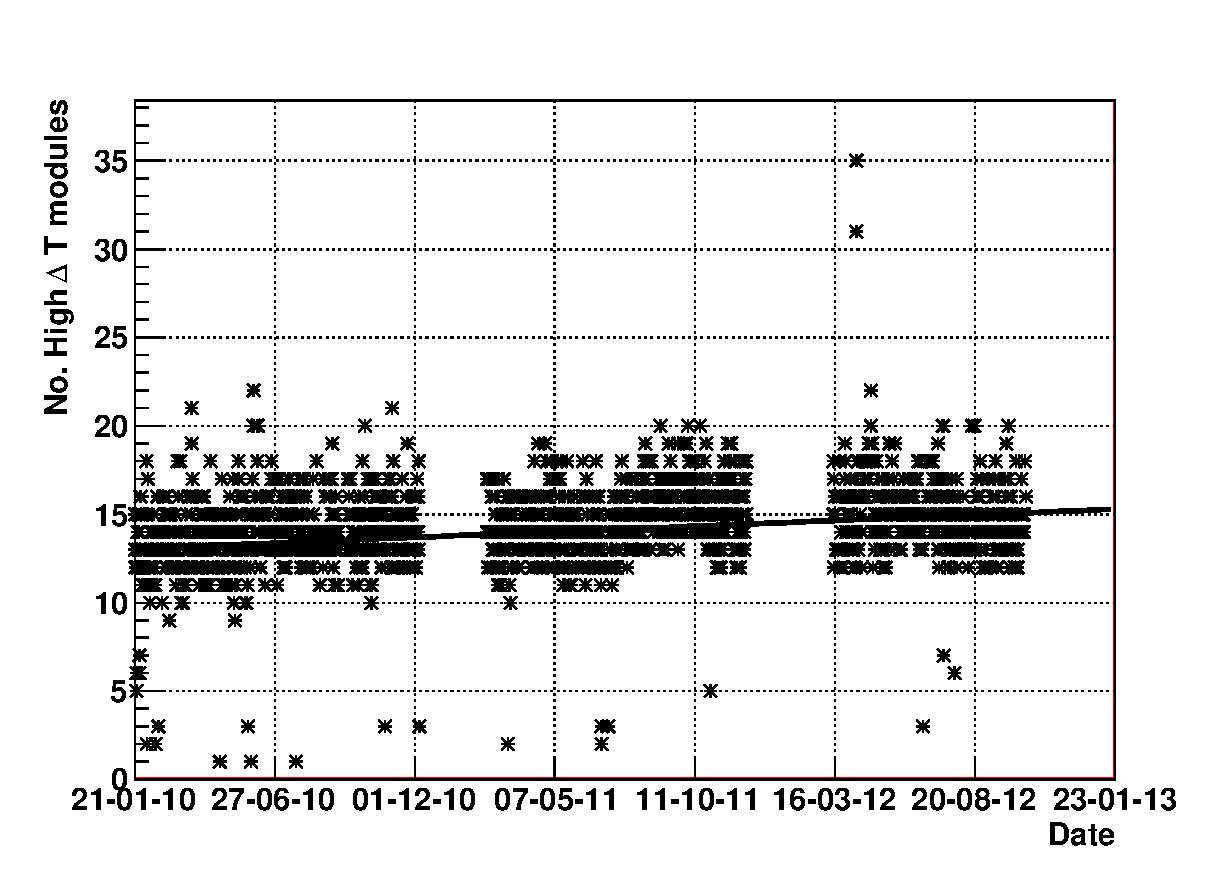
\includegraphics[width=0.47\textwidth]{number_problem_modules/num_high_delta_t}

	}
	\subfigure[]{
		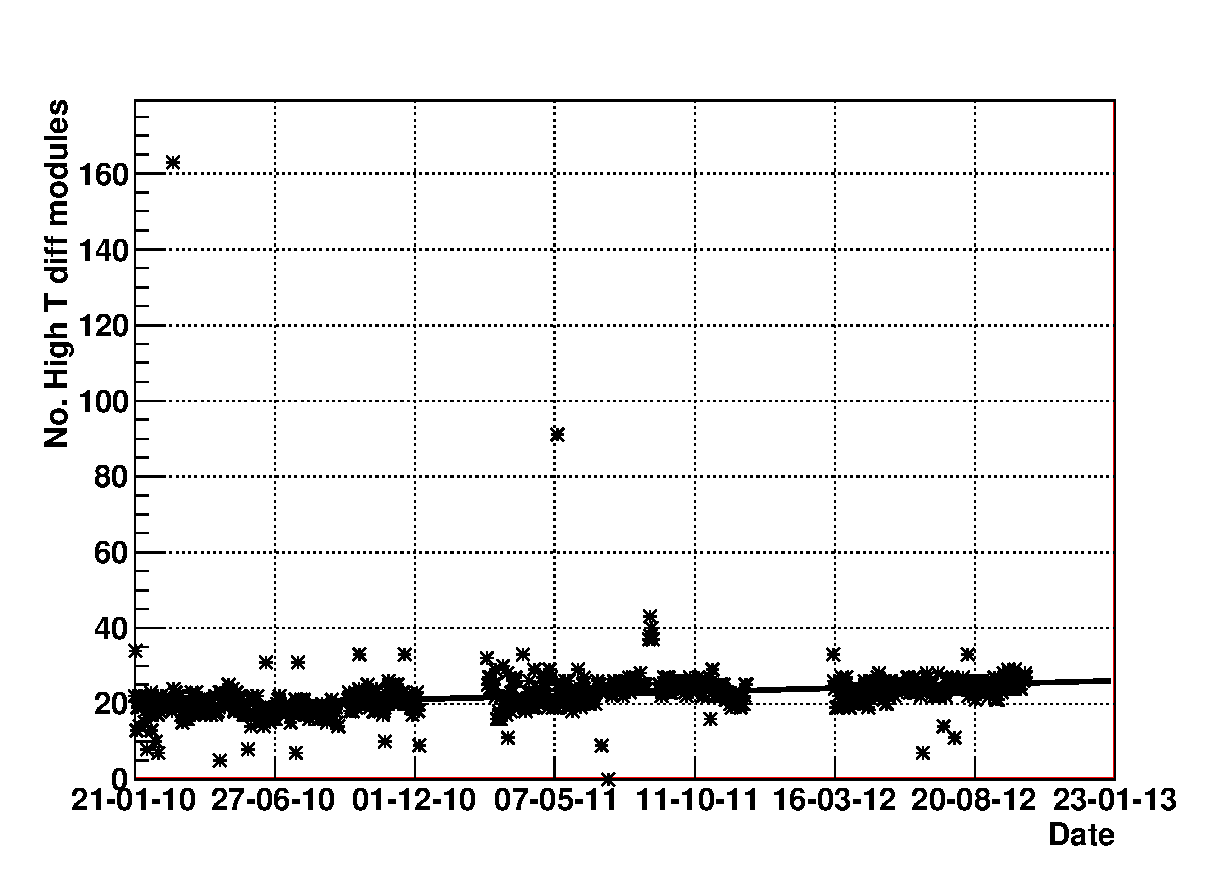
\includegraphics[width=0.47\textwidth]{number_problem_modules/num_high_t_diff}
	}
	\caption{The number of `problematic' modules with (a) \deltat and (b)
        \tdiff of greater magnitude than the problem threshold per day as a
        function of time between 20/01/2010 to 16/10/2012. The number of
        `problematic' modules is not seen to increase significantly as a
        function of time.}
	\label{fig:num_pm}
\end{figure}

\section{Behaviour of problematic modules}

For each of the problematic modules the value of the problematic monitoring variable has been plotted as a function of time for the first six months of 2010 in order to determine whether the problem is getting worse. For most of the problematic modules the magnitude of the monitoring variable does not increase over the period, aside from small fluctuations.  However, one module has been identified with a high \deltat of increasing magnitude, and four modules with a \tdiff of increasing magnitude. A further two show odd behavior. 

\begin{figure}[h]
 	\centering
	\subfigure[]{
		\includegraphics[width=0.47\textwidth]{pm_ev_dt_126-A5}
	}
	\subfigure[]{
		\includegraphics[width=0.47\textwidth]{pm_ev_dt_126-C6}
	}
	\caption{The temperature difference between the front and back of the module (\deltat) for barrel module Q3/B6/L126/I/P29/A5 (left) and barrel module Q3/B6/L126/O/P30/C6 (right) as a function of time between 20/1/2010 to 18/7/2010}
	\label{fig:pm_ev_dt}
\end{figure}

The plot on the left of~\ref{fig:pm_ev_dt} shows the only module with a \deltat of increasing magnitude. The temperature difference between the front and back of the module has increased by about 1.5$^\circ$C in six months, with back of the module warmer than the front. This suggests that the two sides of the module are slowly separating. The plot on the right of~\ref{fig:pm_ev_dt} shows a  module for which \deltat jumps between 0\dc  and 3-4\dc every 1 or 2 months. This suggests an intermittent failure in the integrity of the module, but is very unexpected behaviour and requires further investigation. No other problems with this module have been recorded.

Three modules were observed to have a \tdiff becoming more negative with time, indicating that they are becoming warmer relative to their neighbours by about 1\dc  over six months. This suggests a failure in coupling to the cooling pipe that is getting worse with time. One of these modules is shown on the left of Figure~\ref{fig:pm_ev_tdiff}.  The right hand plot of Figure~\ref{fig:pm_ev_tdiff} shows a module with \tdiff becoming more positive over time, and also showing sharp jumps in the variable. An increasing positive \tdiff means the module is cooler than its neighbours, and becoming even more cooler. This would suggest that the module is running at a lower power, although it is unclear why this would cause the \tdiff to increase over time, nor explain the sudden jumps. Generally modules running at lower power are detected with the DAQ (Data Acquisition) software, but no problem has been reported for this module. A further seven modules with a \tdiff which jumps between 0\dc and around +7 \dc have been observed.  All seven of these modules have other known problems; either the modules do not receive the high voltage, or there is a problem with the module communication. These modules are out of configuration, and data sent from these modules is not used for physics.

\begin{figure}[h]
 	\centering
	\subfigure[]{
		\includegraphics[width=0.47\textwidth]{pm_ev_tdiff_125-A4}
	}
	\subfigure[]{
		\includegraphics[width=0.47\textwidth]{pm_ev_tdiff_160-07}
	}
	\caption{The difference in temperature between the module and its neighbours (\tdiff) as a function of time for module Q2/B5/L102/I/P24/C3 (left) Q4/ECA/D4/L160/RO/07 (right) between 20/1/2010 to 18/7/2010. }
	\label{fig:pm_ev_tdiff}
\end{figure}

\section{Conclusions}

I plan to cross check problem modules against detector conditions and coincidences with events like powercuts, shutdowns, cooling failures etc, as well as studying characteristics of the individual modules such as the voltage arriving at the module. I also plan to cross check problematic modules against the `production database' which details tests made of modules at production to identify any correlations. 

\def\LumiTotalDeliveredTwentyTen{48.1~\ipb}
\def\LumiTotalDeliveredTwentyTwelve{19.9~\ifb}
\def\LumiTotalDeliveredTwentyEleven{5.61~\ifb} % FIXME


\newcommand{\TheoryCxSevenZeroWidth}{??.?? \errSym{?.??}}
\newcommand{\TheoryCxSevenOnShell}{13.33 \errSym{0.01}}
\newcommand{\TheoryCxSevenOnShellFid}{10.60 \errSym{0.01}}
\newcommand{\TheoryCxSevenOffShell}{16.70 \errSym{0.04}}
\newcommand{\TheoryCxSevenOffShellFid}{12.62 \errSym{0.04}}

\newcommand{\TheoryCxSevenZeroWidthCTerrPerc}{\errAsym{ 2.4 \%}{ 2.5 \%}}
\newcommand{\TheoryCxSevenOnShellCTerrPerc}{\errAsym{ 3.0 \%}{ 3.1 \%}}
\newcommand{\TheoryCxSevenOnShellFidCTerrPerc}{\errAsym{ 2.4 \%}{ 2.5 \%}}
\newcommand{\TheoryCxSevenOffShellCTerrPerc}{\errAsym{2.5 \%}{ 2.5 \%}}
\newcommand{\TheoryCxSevenOffShellFidCTerrPerc}{\errAsym{ 2.5 \%}{ 2.6 \%}}

\newcommand{\TheoryCxSevenZeroWidthPDFerrPerc}{\errAsym{ 3.7 \%}{ 2.7 \%}}
\newcommand{\TheoryCxSevenOnShellPDFerrPerc}{\errAsym{ 3.7 \%}{ 2.7 \%}}
\newcommand{\TheoryCxSevenOnShellFidPDFerrPerc}{\errAsym{ 2.7 \%}{ 2.7 \%}}
\newcommand{\TheoryCxSevenOffShellPDFerrPerc}{\errAsym{ 3.5 \%}{ 2.6\%}}
\newcommand{\TheoryCxSevenOffShellFidPDFerrPerc}{\errAsym{ 3.7 \%}{ 2.5 \%}}

\newcommand{\TheoryCxEightZeroWidth}{????? \errSym{????}}
\newcommand{\TheoryCxEightOnShell}{????? \errSym{????}}
\newcommand{\TheoryCxEightOnShellFid}{????? \errSym{????}}
\newcommand{\TheoryCxEightOffShell}{????? \errSym{????}}
\newcommand{\TheoryCxEightOffShellFid}{????? \errSym{????}}

\newcommand{\TheoryCxEightZeroWidthCTerrPerc}{\errAsym{ ??? \%}{ ??? \%}}
\newcommand{\TheoryCxEightOnShellCTerrPerc}{\errAsym{ ??? \%}{ ??? \%}}
\newcommand{\TheoryCxEightOnShellFidCTerrPerc}{\errAsym{ ??? \%}{ ??? \%}}
\newcommand{\TheoryCxEightOffShellCTerrPerc}{\errAsym{??? \%}{ ??? \%}}
\newcommand{\TheoryCxEightOffShellFidCTerrPerc}{\errAsym{ ??? \%}{ ??? \%}}

\newcommand{\TheoryCxEightZeroWidthPDFerrPerc}{\errAsym{ ??? \%}{ ??? \%}}
\newcommand{\TheoryCxEightOnShellPDFerrPerc}{\errAsym{ ??? \%}{ ??? \%}}
\newcommand{\TheoryCxEightOnShellFidPDFerrPerc}{\errAsym{ ??? \%}{ ??? \%}}
\newcommand{\TheoryCxEightOffShellPDFerrPerc}{\errAsym{ ??? \%}{ ???\%}}
\newcommand{\TheoryCxEightOffShellFidPDFerrPerc}{\errAsym{ ??? \%}{ ??? \%}}

\newcommand{\TheoryGGFracSevenZeroWidth}{?? \%}
\newcommand{\TheoryGGFracSevenOnShell}{?? \%}
\newcommand{\TheoryGGFracSevenOnShellFidSevenTeV}{?? \%}
\newcommand{\TheoryGGFracSevenOffShell}{?? \%}
\newcommand{\TheoryGGFracSevenOffShellFidSevenTeV}{?? \%}

\newcommand{\TheoryGGFracEightZeroWidth}{?? \%}
\newcommand{\TheoryGGFracEightOnShell}{?? \%}
\newcommand{\TheoryGGFracEightOnShellFidSevenTeV}{?? \%}
\newcommand{\TheoryGGFracEightOffShell}{?? \%}
\newcommand{\TheoryGGFracEightOffShellFidSevenTeV}{?? \%}

%%%%%%%%%%%%%%%%%%%%%%%%%%%%%%%%%%%%%%%
%~~~~~~~~~~~~~~~~~~~~~~~~~~~~~~~~~~~~~
% Observed Events
% Convenience functions
%~~~~~~~~~~~~~~~~~~~~~~~~~~~~~~~~~~~~~
%%%%%%%%%%%%%%%%%%%%%%%%%%%%%%%%%%%%%%%

%~~~~~~~~~~~~~~~~~~~~~~~~~~~~~~~~~~~~~
% Signal Expectation
\newcommand{\ZZSevenTeVSigExpectation}{\ZZSevenTeVNSigEventsExpectedCentralLLLL\ensuremath{\pm}\ZZSevenTeVNSigEventsExpectedStatLLLL(stat.)\ensuremath{\pm}\ZZSevenTeVNSigEventsExpectedSystLLLL(syst.)}
\newcommand{\ZZSevenTeVSigExpectationEEEE}{\ZZSevenTeVNSigEventsExpectedCentralEEEE\ensuremath{\pm}\ZZSevenTeVNSigEventsExpectedStatEEEE\ensuremath{\pm}\ZZSevenTeVNSigEventsExpectedSystEEEE}
\newcommand{\ZZSevenTeVSigExpectationMMMM}{\ZZSevenTeVNSigEventsExpectedCentralMMMM\ensuremath{\pm}\ZZSevenTeVNSigEventsExpectedStatMMMM\ensuremath{\pm}\ZZSevenTeVNSigEventsExpectedSystMMMM}
\newcommand{\ZZSevenTeVSigExpectationEEMM}{\ZZSevenTeVNSigEventsExpectedCentralEEMM\ensuremath{\pm}\ZZSevenTeVNSigEventsExpectedStatEEMM\ensuremath{\pm}\ZZSevenTeVNSigEventsExpectedSystEEMM}

\newcommand{\ZZSevenTeVSigExpectationOneDp}{\ZZSevenTeVNSigEventsExpectedCentralLLLLOneDp\ensuremath{\pm}\ZZSevenTeVNSigEventsExpectedTotalUncLLLLOneDp}
\newcommand{\ZZSevenTeVSigExpectationEEEEOneDp}{\ZZSevenTeVNSigEventsExpectedCentralEEEEOneDp\ensuremath{\pm}\ZZSevenTeVNSigEventsExpectedTotalUncEEEEOneDp}
\newcommand{\ZZSevenTeVSigExpectationMMMMOneDp}{\ZZSevenTeVNSigEventsExpectedCentralMMMMOneDp\ensuremath{\pm}\ZZSevenTeVNSigEventsExpectedTotalUncMMMMOneDp}
\newcommand{\ZZSevenTeVSigExpectationEEMMOneDp}{\ZZSevenTeVNSigEventsExpectedCentralEEMMOneDp\ensuremath{\pm}\ZZSevenTeVNSigEventsExpectedTotalUncEEMMOneDp}

%~~~~~~~~~~~~~~~~~~~~~~~~~~~~~~~~~~~~~
% Background Estimate
%\newcommand{\ZZSevenTeVDDBgEst}{\ZZSevenTeVDDBgEstCentralLLLL\ZZSevenTeVDDBgEstStatLLLL(stat.)\ZZSevenTeVDDBgEstSystLLLL(syst.)}
\newcommand{\ZZSevenTeVDDBgEst}{\ZZSevenTeVDDBgEstCentralLLLL\ZZSevenTeVDDBgEstStatLLLL\ZZSevenTeVDDBgEstSystLLLL}
\newcommand{\ZZSevenTeVDDBgEstEEEE}{\ZZSevenTeVDDBgEstCentralEEEE\ZZSevenTeVDDBgEstStatEEEE\ZZSevenTeVDDBgEstSystEEEE}
\newcommand{\ZZSevenTeVDDBgEstEEMM}{\ZZSevenTeVDDBgEstCentralEEMM\ZZSevenTeVDDBgEstStatEEMM\ZZSevenTeVDDBgEstSystEEMM}
\newcommand{\ZZSevenTeVDDBgEstMMMM}{\ZZSevenTeVDDBgEstCentralMMMM\ZZSevenTeVDDBgEstStatMMMM\ZZSevenTeVDDBgEstSystMMMM}

\newcommand{\ZZSevenTeVDDBgEstOneDpErrType}{\ZZSevenTeVDDBgEstCentralLLLLOneDp\ensuremath{ }\ZZSevenTeVDDBgEstStatLLLLOneDp\ensuremath{ }(stat.)\ZZSevenTeVDDBgEstSystLLLLOneDp\ensuremath{ }(syst.)}
\newcommand{\ZZSevenTeVDDBgEstOneDp}{\ZZSevenTeVDDBgEstCentralLLLLOneDp\ZZSevenTeVDDBgEstStatLLLLOneDp\ZZSevenTeVDDBgEstSystLLLLOneDp}
\newcommand{\ZZSevenTeVDDBgEstEEEEOneDp}{\ZZSevenTeVDDBgEstCentralEEEEOneDp\ZZSevenTeVDDBgEstStatEEEEOneDp\ZZSevenTeVDDBgEstSystEEEEOneDp}
\newcommand{\ZZSevenTeVDDBgEstEEMMOneDp}{\ZZSevenTeVDDBgEstCentralEEMMOneDp\ZZSevenTeVDDBgEstStatEEMMOneDp\ZZSevenTeVDDBgEstSystEEMMOneDp}
\newcommand{\ZZSevenTeVDDBgEstMMMMOneDp}{\ZZSevenTeVDDBgEstCentralMMMMOneDp\ZZSevenTeVDDBgEstStatMMMMOneDp\ZZSevenTeVDDBgEstSystMMMMOneDp}


%~~~~~~~~~~~~~~~~~~~~~~~~~~~~~~~~~~~~~
% Total Cross Section 
\newcommand{\ZZSevenTeVTotalCrossSection}{\ZZSevenTeVTotalCrossSectionGaussian}
\newcommand{\ZZSevenTeVTotalCrossSectionOneDp}{\ZZSevenTeVTotalCrossSectionGaussianOneDp}

%~~~~~~~~~~~~~~~~~~~~~~~~~~~~~~~~~~~~~
% Total Cross Gamma 
\newcommand{\ZZSevenTeVTotalCrossSectionGamma}{\ensuremath{\ZZSevenTeVTotalCrossSectionGammaCentral^{+\ZZSevenTeVTotalCrossSectionGammaStatUp}_{-\ZZSevenTeVTotalCrossSectionGammaStatDown}\textrm{(stat.)}^{+\ZZSevenTeVTotalCrossSectionGammaSystUp}_{-\ZZSevenTeVTotalCrossSectionGammaSystDown}\textrm{(syst.)}\pm\ZZSevenTeVTotalCrossSectionGammaLumiUnc\textrm{(lumi.) pb}}}
\newcommand{\ZZSevenTeVTotalCrossSectionGammaOneDp}{\ensuremath{\ZZSevenTeVTotalCrossSectionGammaCentralOneDp^{+\ZZSevenTeVTotalCrossSectionGammaStatUpOneDp}_{-\ZZSevenTeVTotalCrossSectionGammaStatDownOneDp}\textrm{(stat.)}^{+\ZZSevenTeVTotalCrossSectionGammaSystUpOneDp}_{-\ZZSevenTeVTotalCrossSectionGammaSystDownOneDp}\textrm{(syst.)}\pm\ZZSevenTeVTotalCrossSectionGammaLumiUncOneDp\textrm{(lumi.) pb}}}

%~~~~~~~~~~~~~~~~~~~~~~~~~~~~~~~~~~~~~
% Total Cross Gaussian 
\newcommand{\ZZSevenTeVTotalCrossSectionGaussian}{\ensuremath{\ZZSevenTeVTotalCrossSectionGaussianCentral^{+\ZZSevenTeVTotalCrossSectionGaussianStatUp}_{-\ZZSevenTeVTotalCrossSectionGaussianStatDown}\textrm{(stat.)}^{+\ZZSevenTeVTotalCrossSectionGaussianSystUp}_{-\ZZSevenTeVTotalCrossSectionGaussianSystDown}\textrm{(syst.)}\pm\ZZSevenTeVTotalCrossSectionGaussianLumiUnc\textrm{(lumi.) pb}}}

%~~~~~~~~~~~~~~~~~~~~~~~~~~~~~~~~~~~~~
% Fiducial cross section ZZ*
\newcommand{\ZZSevenTeVFiducialCrossSectionZZsLLLL}{\ZZSevenTeVFiducialCrossSectionZZsLLLLGaussian}
\newcommand{\ZZSevenTeVFiducialCrossSectionZZsEEEE}{\ZZSevenTeVFiducialCrossSectionZZsEEEEGaussian}
\newcommand{\ZZSevenTeVFiducialCrossSectionZZsMMMM}{\ZZSevenTeVFiducialCrossSectionZZsMMMMGaussian}
\newcommand{\ZZSevenTeVFiducialCrossSectionZZsEEMM}{\ZZSevenTeVFiducialCrossSectionZZsEEMMGaussian}

\newcommand {\ZZSevenTeVFiducialCrossSectionZZsLLLLGaussian}{\measStatSystLumi
            {\ZZSevenTeVFiducialCrossSectionZZsLLLLGaussianCentral}{\errAsym
            {\ZZSevenTeVFiducialCrossSectionZZsLLLLGaussianStatUp}
            {\ZZSevenTeVFiducialCrossSectionZZsLLLLGaussianStatDown}}{\errAsym
            {\ZZSevenTeVFiducialCrossSectionZZsLLLLGaussianSystUp}
            {\ZZSevenTeVFiducialCrossSectionZZsLLLLGaussianSystDown}}{\errSym
            {\ZZSevenTeVFiducialCrossSectionZZsLLLLGaussianLumiUnc}}~fb}

\newcommand {\ZZSevenTeVFiducialCrossSectionZZsEEEEGaussian}{\measStatSystLumi
            {\ZZSevenTeVFiducialCrossSectionZZsEEEEGaussianCentral}{\errAsym
            {\ZZSevenTeVFiducialCrossSectionZZsEEEEGaussianStatUp}
            {\ZZSevenTeVFiducialCrossSectionZZsEEEEGaussianStatDown}}{\errAsym
            {\ZZSevenTeVFiducialCrossSectionZZsEEEEGaussianSystUp}
            {\ZZSevenTeVFiducialCrossSectionZZsEEEEGaussianSystDown}}{\errSym
            {\ZZSevenTeVFiducialCrossSectionZZsEEEEGaussianLumiUnc}}~fb}

\newcommand {\ZZSevenTeVFiducialCrossSectionZZsMMMMGaussian}{\measStatSystLumi
            {\ZZSevenTeVFiducialCrossSectionZZsMMMMGaussianCentral}{\errAsym
            {\ZZSevenTeVFiducialCrossSectionZZsMMMMGaussianStatUp}
            {\ZZSevenTeVFiducialCrossSectionZZsMMMMGaussianStatDown}}{\errAsym
            {\ZZSevenTeVFiducialCrossSectionZZsMMMMGaussianSystUp}
            {\ZZSevenTeVFiducialCrossSectionZZsMMMMGaussianSystDown}}{\errSym
            {\ZZSevenTeVFiducialCrossSectionZZsMMMMGaussianLumiUnc}}~fb}

\newcommand {\ZZSevenTeVFiducialCrossSectionZZsEEMMGaussian}{\measStatSystLumi
            {\ZZSevenTeVFiducialCrossSectionZZsEEMMGaussianCentral}{\errAsym
            {\ZZSevenTeVFiducialCrossSectionZZsEEMMGaussianStatUp}
            {\ZZSevenTeVFiducialCrossSectionZZsEEMMGaussianStatDown}}{\errAsym
            {\ZZSevenTeVFiducialCrossSectionZZsEEMMGaussianSystUp}
            {\ZZSevenTeVFiducialCrossSectionZZsEEMMGaussianSystDown}}{\errSym
            {\ZZSevenTeVFiducialCrossSectionZZsEEMMGaussianLumiUnc}}~fb}

%~~~~~~~~~~~~~~~~~~~~~~~~~~~~~~~~~~~~~
% Fiducial cross section ZZ
\newcommand{\ZZSevenTeVFiducialCrossSectionZZLLLL}{\ZZSevenTeVFiducialCrossSectionZZLLLLGaussian}
\newcommand{\ZZSevenTeVFiducialCrossSectionZZEEEE}{\ZZSevenTeVFiducialCrossSectionZZEEEEGaussian}
\newcommand{\ZZSevenTeVFiducialCrossSectionZZMMMM}{\ZZSevenTeVFiducialCrossSectionZZMMMMGaussian}
\newcommand{\ZZSevenTeVFiducialCrossSectionZZEEMM}{\ZZSevenTeVFiducialCrossSectionZZEEMMGaussian}

\newcommand {\ZZSevenTeVFiducialCrossSectionZZLLLLGaussian}{\measStatSystLumi
            {\ZZSevenTeVFiducialCrossSectionZZLLLLGaussianCentral}{\errAsym
            {\ZZSevenTeVFiducialCrossSectionZZLLLLGaussianStatUp}
            {\ZZSevenTeVFiducialCrossSectionZZLLLLGaussianStatDown}}{\errAsym
            {\ZZSevenTeVFiducialCrossSectionZZLLLLGaussianSystUp}
            {\ZZSevenTeVFiducialCrossSectionZZLLLLGaussianSystDown}}{\errSym
            {\ZZSevenTeVFiducialCrossSectionZZLLLLGaussianLumiUnc}}~fb}

\newcommand {\ZZSevenTeVFiducialCrossSectionZZEEEEGaussian}{\measStatSystLumi
            {\ZZSevenTeVFiducialCrossSectionZZEEEEGaussianCentral}{\errAsym
            {\ZZSevenTeVFiducialCrossSectionZZEEEEGaussianStatUp}
            {\ZZSevenTeVFiducialCrossSectionZZEEEEGaussianStatDown}}{\errAsym
            {\ZZSevenTeVFiducialCrossSectionZZEEEEGaussianSystUp}
            {\ZZSevenTeVFiducialCrossSectionZZEEEEGaussianSystDown}}{\errSym
            {\ZZSevenTeVFiducialCrossSectionZZEEEEGaussianLumiUnc}}~fb}

\newcommand {\ZZSevenTeVFiducialCrossSectionZZMMMMGaussian}{\measStatSystLumi
            {\ZZSevenTeVFiducialCrossSectionZZMMMMGaussianCentral}{\errAsym
            {\ZZSevenTeVFiducialCrossSectionZZMMMMGaussianStatUp}
            {\ZZSevenTeVFiducialCrossSectionZZMMMMGaussianStatDown}}{\errAsym
            {\ZZSevenTeVFiducialCrossSectionZZMMMMGaussianSystUp}
            {\ZZSevenTeVFiducialCrossSectionZZMMMMGaussianSystDown}}{\errSym
            {\ZZSevenTeVFiducialCrossSectionZZMMMMGaussianLumiUnc}}~fb}

\newcommand {\ZZSevenTeVFiducialCrossSectionZZEEMMGaussian}{\measStatSystLumi
            {\ZZSevenTeVFiducialCrossSectionZZEEMMGaussianCentral}{\errAsym
            {\ZZSevenTeVFiducialCrossSectionZZEEMMGaussianStatUp}
            {\ZZSevenTeVFiducialCrossSectionZZEEMMGaussianStatDown}}{\errAsym
            {\ZZSevenTeVFiducialCrossSectionZZEEMMGaussianSystUp}
            {\ZZSevenTeVFiducialCrossSectionZZEEMMGaussianSystDown}}{\errSym
            {\ZZSevenTeVFiducialCrossSectionZZEEMMGaussianLumiUnc}}~fb}

%~~~~~~~~~~~~~~~~~~~~~~~~~~~~~~~~~~~~~
% Theory Fiducial cross section ZZ
\newcommand{\ZZSevenTeVTheoryFiducialCrossSectionZZLLLL}{
           {\ZZSevenTeVTheoryFiducialCrossSectionZZLLLLCentral\errAsym
           {\ZZSevenTeVTheoryFiducialCrossSectionZZLLLLErrUp}
           {\ZZSevenTeVTheoryFiducialCrossSectionZZLLLLErrDown}~fb}}

\newcommand{\ZZSevenTeVTheoryFiducialCrossSectionZZEEEE}{
           {\ZZSevenTeVTheoryFiducialCrossSectionZZEEEECentral\errAsym
           {\ZZSevenTeVTheoryFiducialCrossSectionZZEEEEErrUp}
           {\ZZSevenTeVTheoryFiducialCrossSectionZZEEEEErrDown}~fb}}

%\newcommand{\ZZSevenTeVTheoryFiducialCrossSectionZZMMMM}{
           %{\ZZSevenTeVTheoryFiducialCrossSectionZZMMMMCentral\errAsym
           %{\ZZSevenTeVTheoryFiducialCrossSectionZZMMMMErrUp}
           %{\ZZSevenTeVTheoryFiducialCrossSectionZZMMMMErrDown}~fb}}

\newcommand{\ZZSevenTeVTheoryFiducialCrossSectionZZMMMM}{
           {\FPdiv\p{\TheoryCxSevenOnShellFidSevenTeV}{2} 
           \FPprint\p 
           \errAsym
           {\TheoryCxSevenOnShellFidSevenTeVTheoryErrAbsUp}
           {\TheoryCxSevenOnShellFidSevenTeVTheoryErrAbsDown}~fb}}

\newcommand{\ZZSevenTeVTheoryFiducialCrossSectionZZEEMM}{
           {\TheoryCxSevenOnShellFidSevenTeV\errAsym
           {\TheoryCxSevenOnShellFidSevenTeVTheoryErrAbsUp}
           {\TheoryCxSevenOnShellFidSevenTeVTheoryErrAbsDown}~fb}}

%~~~~~~~~~~~~~~~~~~~~~~~~~~~~~~~~~~~~~
% Theory Fiducial cross section ZZ*
\newcommand{\ZZSevenTeVTheoryFiducialCrossSectionZZsLLLL}{
           {\ZZSevenTeVTheoryFiducialCrossSectionZZsLLLLCentral\errAsym
           {\ZZSevenTeVTheoryFiducialCrossSectionZZsLLLLErrUp}
           {\ZZSevenTeVTheoryFiducialCrossSectionZZsLLLLErrDown}~fb}}

\newcommand{\ZZSevenTeVTheoryFiducialCrossSectionZZsEEEE}{
           {\ZZSevenTeVTheoryFiducialCrossSectionZZsEEEECentral\errAsym
           {\ZZSevenTeVTheoryFiducialCrossSectionZZsEEEEErrUp}
           {\ZZSevenTeVTheoryFiducialCrossSectionZZsEEEEErrDown}~fb}}

\newcommand{\ZZSevenTeVTheoryFiducialCrossSectionZZsMMMM}{
           {\ZZSevenTeVTheoryFiducialCrossSectionZZsMMMMCentral\errAsym
           {\ZZSevenTeVTheoryFiducialCrossSectionZZsMMMMErrUp}
           {\ZZSevenTeVTheoryFiducialCrossSectionZZsMMMMErrDown}~fb}}

\newcommand{\ZZSevenTeVTheoryFiducialCrossSectionZZsEEMM}{
           {\ZZSevenTeVTheoryFiducialCrossSectionZZsEEMMCentral\errAsym
           {\ZZSevenTeVTheoryFiducialCrossSectionZZsEEMMErrUp}
           {\ZZSevenTeVTheoryFiducialCrossSectionZZsEEMMErrDown}~fb}}

%~~~~~~~~~~~~~~~~~~~~~~~~~~~~~~~~~~~~~
% Theory Total cross section ZZ
\newcommand{\ZZSevenTeVTheoryTotalCrossSection}{\ensuremath{\ZZSevenTeVTheoryTotalCrossSectionCentral^{+\ZZSevenTeVTheoryTotalCrossSectionSystUp}_{-\ZZSevenTeVTheoryTotalCrossSectionSystDown}\textrm{ pb}}}


\newcommand{\ZZSevenTeVTheoryTotalCrossSectionOneDp}{\ensuremath{\ZZSevenTeVTheoryTotalCrossSectionCentralOneDp\pm\ZZSevenTeVTheoryTotalCrossSectionSystOneDp\textrm{ pb}}}

%~~~~~~~~~~~~~~~~~~~~~~~~~~~~~~~~~~~~~

%%%%%%%%%%%%%%%%%%%%%%%%%%%%%%%%%%%%%%%
%~~~~~~~~~~~~~~~~~~~~~~~~~~~~~~~~~~~~~
% Observed Events
%~~~~~~~~~~~~~~~~~~~~~~~~~~~~~~~~~~~~~
%%%%%%%%%%%%%%%%%%%%%%%%%%%%%%%%%%%%%%%

%~~~~~~~~~~~~~~~~~~~~~~~~~~~~~~~~~~~~~
% Number of observed events
% Added 19/1/2013 from 7TeVSup
% ZZ
\def\ZZSevenTeVNObsZZEEEE{16}
\def\ZZSevenTeVNObsZZMMMM{23}
\def\ZZSevenTeVNObsZZEEMM{27}
\def\ZZSevenTeVNObsZZLLLL{66}

% ZZ*
\def\ZZSevenTeVNObsZZsEEEE{21}
\def\ZZSevenTeVNObsZZsMMMM{30}
\def\ZZSevenTeVNObsZZsEEMM{33}
\def\ZZSevenTeVNObsZZsLLLL{84}
%~~~~~~~~~~~~~~~~~~~~~~~~~~~~~~~~~~~~~

%%%%%%%%%%%%%%%%%%%%%%%%%%%%%%%%%%%%%%%
%~~~~~~~~~~~~~~~~~~~~~~~~~~~~~~~~~~~~~
% Cross Sections
%~~~~~~~~~~~~~~~~~~~~~~~~~~~~~~~~~~~~~
%%%%%%%%%%%%%%%%%%%%%%%%%%%%%%%%%%%%%%%

%~~~~~~~~~~~~~~~~~~~~~~~~~~~~~~~~~~~~~
% Total Cross Section (pb) GAMMA
% Updated: 
\def\ZZSevenTeVTotalCrossSectionGammaCentral{x.xx}
\def\ZZSevenTeVTotalCrossSectionGammaStatUp{x.xx}
\def\ZZSevenTeVTotalCrossSectionGammaStatDown{x.xx}
\def\ZZSevenTeVTotalCrossSectionGammaSystUp{x.xx}
\def\ZZSevenTeVTotalCrossSectionGammaSystDown{x.xx}
\def\ZZSevenTeVTotalCrossSectionGammaLumiUnc{x.xx}

% ~ To 1dp
\def\ZZSevenTeVTotalCrossSectionGammaCentralOneDp{x.x}
\def\ZZSevenTeVTotalCrossSectionGammaStatUpOneDp{x.x}
\def\ZZSevenTeVTotalCrossSectionGammaStatDownOneDp{x.x}
\def\ZZSevenTeVTotalCrossSectionGammaSystUpOneDp{x.x}
\def\ZZSevenTeVTotalCrossSectionGammaSystDownOneDp{x.x}
\def\ZZSevenTeVTotalCrossSectionGammaLumiUncOneDp{x.x}
%~~~~~~~~~~~~~~~~~~~~~~~~~~~~~~~~~~~~~

%~~~~~~~~~~~~~~~~~~~~~~~~~~~~~~~~~~~~~
% Total Cross Section (pb) GAMMA
% Updated: 
\def\ZZSevenTeVTotalCrossSectionGaussianCentral{x.xx}
\def\ZZSevenTeVTotalCrossSectionGaussianStatUp{x.xx}
\def\ZZSevenTeVTotalCrossSectionGaussianStatDown{x.xx}
\def\ZZSevenTeVTotalCrossSectionGaussianSystUp{x.xx}
\def\ZZSevenTeVTotalCrossSectionGaussianSystDown{x.xx}
\def\ZZSevenTeVTotalCrossSectionGaussianLumiUnc{x.xx}
%~~~~~~~~~~~~~~~~~~~~~~~~~~~~~~~~~~~~~

%~~~~~~~~~~~~~~~~~~~~~~~~~~~~~~~~~~~~~
%~~~~~~~~~~~~~~~~~~~~~~~~~~~~~~~~~~~~~
% Fiducial Cross Section (fb) ZZ GAUSSIAN
\def\ZZSevenTeVFiducialCrossSectionZZLLLLGaussianCentral{x.xx}
\def\ZZSevenTeVFiducialCrossSectionZZLLLLGaussianStatUp{x.xx}
\def\ZZSevenTeVFiducialCrossSectionZZLLLLGaussianStatDown{x.xx}
\def\ZZSevenTeVFiducialCrossSectionZZLLLLGaussianSystUp{x.xx}
\def\ZZSevenTeVFiducialCrossSectionZZLLLLGaussianSystDown{x.xx}
\def\ZZSevenTeVFiducialCrossSectionZZLLLLGaussianLumiUnc{x.xx}

\def\ZZSevenTeVFiducialCrossSectionZZEEEEGaussianCentral{x.xx}
\def\ZZSevenTeVFiducialCrossSectionZZEEEEGaussianStatUp{x.xx}
\def\ZZSevenTeVFiducialCrossSectionZZEEEEGaussianStatDown{x.xx}
\def\ZZSevenTeVFiducialCrossSectionZZEEEEGaussianSystUp{x.xx}
\def\ZZSevenTeVFiducialCrossSectionZZEEEEGaussianSystDown{x.xx}
\def\ZZSevenTeVFiducialCrossSectionZZEEEEGaussianLumiUnc{x.xx}

\def\ZZSevenTeVFiducialCrossSectionZZMMMMGaussianCentral{x.xx}
\def\ZZSevenTeVFiducialCrossSectionZZMMMMGaussianStatUp{x.xx}
\def\ZZSevenTeVFiducialCrossSectionZZMMMMGaussianStatDown{x.xx}
\def\ZZSevenTeVFiducialCrossSectionZZMMMMGaussianSystUp{x.xx}
\def\ZZSevenTeVFiducialCrossSectionZZMMMMGaussianSystDown{x.xx}
\def\ZZSevenTeVFiducialCrossSectionZZMMMMGaussianLumiUnc{x.xx}

\def\ZZSevenTeVFiducialCrossSectionZZEEMMGaussianCentral{x.xx}
\def\ZZSevenTeVFiducialCrossSectionZZEEMMGaussianStatUp{x.xx}
\def\ZZSevenTeVFiducialCrossSectionZZEEMMGaussianStatDown{x.xx}
\def\ZZSevenTeVFiducialCrossSectionZZEEMMGaussianSystUp{x.xx}
\def\ZZSevenTeVFiducialCrossSectionZZEEMMGaussianSystDown{x.xx}
\def\ZZSevenTeVFiducialCrossSectionZZEEMMGaussianLumiUnc{x.xx}

% Fiducial Cross Section (fb) ZZ* GAUSSIAN
\def\ZZSevenTeVFiducialCrossSectionZZsLLLLGaussianCentral{x.xx}
\def\ZZSevenTeVFiducialCrossSectionZZsLLLLGaussianStatUp{x.xx}
\def\ZZSevenTeVFiducialCrossSectionZZsLLLLGaussianStatDown{x.xx}
\def\ZZSevenTeVFiducialCrossSectionZZsLLLLGaussianSystUp{x.xx}
\def\ZZSevenTeVFiducialCrossSectionZZsLLLLGaussianSystDown{x.xx}
\def\ZZSevenTeVFiducialCrossSectionZZsLLLLGaussianLumiUnc{x.xx}

\def\ZZSevenTeVFiducialCrossSectionZZsEEEEGaussianCentral{x.xx}
\def\ZZSevenTeVFiducialCrossSectionZZsEEEEGaussianStatUp{x.xx}
\def\ZZSevenTeVFiducialCrossSectionZZsEEEEGaussianStatDown{x.xx}
\def\ZZSevenTeVFiducialCrossSectionZZsEEEEGaussianSystUp{x.xx}
\def\ZZSevenTeVFiducialCrossSectionZZsEEEEGaussianSystDown{x.xx}
\def\ZZSevenTeVFiducialCrossSectionZZsEEEEGaussianLumiUnc{x.xx}

\def\ZZSevenTeVFiducialCrossSectionZZsMMMMGaussianCentral{x.xx}
\def\ZZSevenTeVFiducialCrossSectionZZsMMMMGaussianStatUp{x.xx}
\def\ZZSevenTeVFiducialCrossSectionZZsMMMMGaussianStatDown{x.xx}
\def\ZZSevenTeVFiducialCrossSectionZZsMMMMGaussianSystUp{x.xx}
\def\ZZSevenTeVFiducialCrossSectionZZsMMMMGaussianSystDown{x.xx}
\def\ZZSevenTeVFiducialCrossSectionZZsMMMMGaussianLumiUnc{x.xx}

\def\ZZSevenTeVFiducialCrossSectionZZsEEMMGaussianCentral{x.xx}
\def\ZZSevenTeVFiducialCrossSectionZZsEEMMGaussianStatUp{x.xx}
\def\ZZSevenTeVFiducialCrossSectionZZsEEMMGaussianStatDown{x.xx}
\def\ZZSevenTeVFiducialCrossSectionZZsEEMMGaussianSystUp{x.xx}
\def\ZZSevenTeVFiducialCrossSectionZZsEEMMGaussianSystDown{x.xx}
\def\ZZSevenTeVFiducialCrossSectionZZsEEMMGaussianLumiUnc{x.xx}
%~~~~~~~~~~~~~~~~~~~~~~~~~~~~~~~~~~~~~

%~~~~~~~~~~~~~~~~~~~~~~~~~~~~~~~~~~~~~
% Theory Fiducial Cross Section (fb) ZZ 
\def\ZZSevenTeVTheoryFiducialCrossSectionZZLLLLCentral{x.xx}
\def\ZZSevenTeVTheoryFiducialCrossSectionZZLLLLErrUp{x.xx}
\def\ZZSevenTeVTheoryFiducialCrossSectionZZLLLLErrDown{x.xx}

\def\ZZSevenTeVTheoryFiducialCrossSectionZZEEEECentral{x.xx}
\def\ZZSevenTeVTheoryFiducialCrossSectionZZEEEEErrUp{x.xx}
\def\ZZSevenTeVTheoryFiducialCrossSectionZZEEEEErrDown{x.xx}

\def\ZZSevenTeVTheoryFiducialCrossSectionZZMMMMCentral{x.xx}
\def\ZZSevenTeVTheoryFiducialCrossSectionZZMMMMErrUp{x.xx}
\def\ZZSevenTeVTheoryFiducialCrossSectionZZMMMMErrDown{x.xx}

\def\ZZSevenTeVTheoryFiducialCrossSectionZZEEMMCentral{x.xx}
\def\ZZSevenTeVTheoryFiducialCrossSectionZZEEMMErrUp{x.xx}
\def\ZZSevenTeVTheoryFiducialCrossSectionZZEEMMErrDown{x.xx}
%~~~~~~~~~~~~~~~~~~~~~~~~~~~~~~~~~~~~~

%~~~~~~~~~~~~~~~~~~~~~~~~~~~~~~~~~~~~~
% Theory Fiducial Cross Section (fb) ZZ *
\def\ZZSevenTeVTheoryFiducialCrossSectionZZsLLLLCentral{x.xx}
\def\ZZSevenTeVTheoryFiducialCrossSectionZZsLLLLErrUp{x.xx}
\def\ZZSevenTeVTheoryFiducialCrossSectionZZsLLLLErrDown{x.xx}

\def\ZZSevenTeVTheoryFiducialCrossSectionZZsEEEECentral{x.xx}
\def\ZZSevenTeVTheoryFiducialCrossSectionZZsEEEEErrUp{x.xx}
\def\ZZSevenTeVTheoryFiducialCrossSectionZZsEEEEErrDown{x.xx}

\def\ZZSevenTeVTheoryFiducialCrossSectionZZsMMMMCentral{x.xx}
\def\ZZSevenTeVTheoryFiducialCrossSectionZZsMMMMErrUp{x.xx}
\def\ZZSevenTeVTheoryFiducialCrossSectionZZsMMMMErrDown{x.xx}

\def\ZZSevenTeVTheoryFiducialCrossSectionZZsEEMMCentral{x.xx}
\def\ZZSevenTeVTheoryFiducialCrossSectionZZsEEMMErrUp{x.xx}
\def\ZZSevenTeVTheoryFiducialCrossSectionZZsEEMMErrDown{x.xx}
%~~~~~~~~~~~~~~~~~~~~~~~~~~~~~~~~~~~~~

%%%%%%%%%%%%%%%%%%%%%%%%%%%%%%%%%%%%%%%
%~~~~~~~~~~~~~~~~~~~~~~~~~~~~~~~~~~~~~
% Expected Events
%~~~~~~~~~~~~~~~~~~~~~~~~~~~~~~~~~~~~~
%%%%%%%%%%%%%%%%%%%%%%%%%%%%%%%%%%%%%%%

%~~~~~~~~~~~~~~~~~~~~~~~~~~~~~~~~~~~~~
% Signal Expectation
\def\ZZSevenTeVNSigEventsExpectedCentralEEEE{x.xx}
\def\ZZSevenTeVNSigEventsExpectedCentralEEMM{x.xx}
\def\ZZSevenTeVNSigEventsExpectedCentralMMMM{x.xx}
\def\ZZSevenTeVNSigEventsExpectedCentralLLLL{x.xx}

\def\ZZSevenTeVNSigEventsExpectedStatEEEE{x.xx}
\def\ZZSevenTeVNSigEventsExpectedStatEEMM{x.xx}
\def\ZZSevenTeVNSigEventsExpectedStatMMMM{x.xx}
\def\ZZSevenTeVNSigEventsExpectedStatLLLL{x.xx}

\def\ZZSevenTeVNSigEventsExpectedSystEEEE{x.xx}
\def\ZZSevenTeVNSigEventsExpectedSystEEMM{x.xx}
\def\ZZSevenTeVNSigEventsExpectedSystMMMM{x.xx}
\def\ZZSevenTeVNSigEventsExpectedSystLLLL{x.xx}

% One dp
\def\ZZSevenTeVNSigEventsExpectedCentralEEEEOneDp{x.x}
\def\ZZSevenTeVNSigEventsExpectedCentralEEMMOneDp{x.x}
\def\ZZSevenTeVNSigEventsExpectedCentralMMMMOneDp{x.x}
\def\ZZSevenTeVNSigEventsExpectedCentralLLLLOneDp{x.x}

\def\ZZSevenTeVNSigEventsExpectedStatEEEEOneDp{x.x}
\def\ZZSevenTeVNSigEventsExpectedStatEEMMOneDp{x.x}
\def\ZZSevenTeVNSigEventsExpectedStatMMMMOneDp{x.x}
\def\ZZSevenTeVNSigEventsExpectedStatLLLLOneDp{x.x}

\def\ZZSevenTeVNSigEventsExpectedSystEEEEOneDp{x.x}
\def\ZZSevenTeVNSigEventsExpectedSystEEMMOneDp{x.x}
\def\ZZSevenTeVNSigEventsExpectedSystMMMMOneDp{x.x}
\def\ZZSevenTeVNSigEventsExpectedSystLLLLOneDp{x.x}

\def\ZZSevenTeVNSigEventsExpectedTotalUncEEEEOneDp{x.x}
\def\ZZSevenTeVNSigEventsExpectedTotalUncEEMMOneDp{x.x}
\def\ZZSevenTeVNSigEventsExpectedTotalUncMMMMOneDp{x.x}
\def\ZZSevenTeVNSigEventsExpectedTotalUncLLLLOneDp{x.x}
%~~~~~~~~~~~~~~~~~~~~~~~~~~~~~~~~~~~~~

%%%%%%%%%%%%%%%%%%%%%%%%%%%%%%%%%%%%%%%
%~~~~~~~~~~~~~~~~~~~~~~~~~~~~~~~~~~~~~
% A_ZZ
%~~~~~~~~~~~~~~~~~~~~~~~~~~~~~~~~~~~~~
%%%%%%%%%%%%%%%%%%%%%%%%%%%%%%%%%%%%%%%

%~~~~~~~~~~~~~~~~~~~~~~~~~~~~~~~~~~~~~
% A_ZZSevenTeV and uncertainties
% Updated: Nick, 1/6/2012
\def\ZZSevenTeVAZZCentral{0.500}
\def\ZZSevenTeVAZZStatUnc{0.001}
\def\ZZSevenTeVAZZSystUnc{0.012}
\def\ZZSevenTeVAZZScaleUncPercentage{0.4}
\def\ZZSevenTeVAZZPDFUncPercentage{2.1}
\def\ZZSevenTeVAZZPDFScaleUncPercentage{2.1}
\def\ZZSevenTeVAZZISRUncPercentage{1.0}
\def\ZZSevenTeVAZZTotalUncPercentage{2.3}
%~~~~~~~~~~~~~~~~~~~~~~~~~~~~~~~~~~~~~

%%%%%%%%%%%%%%%%%%%%%%%%%%%%%%%%%%%%%%%
%~~~~~~~~~~~~~~~~~~~~~~~~~~~~~~~~~~~~~
% C_ZZ
%~~~~~~~~~~~~~~~~~~~~~~~~~~~~~~~~~~~~~
%%%%%%%%%%%%%%%%%%%%%%%%%%%%%%%%%%%%%%%

%~~~~~~~~~~~~~~~~~~~~~~~~~~~~~~~~~~~~~
% CZZ SevenTeV
% Corrected to 7 TeV, 20/1/2013, src=ZZ 7TeV Paper Suport
%% ZZ
\def\ZZSevenTeVCzzZZEEEE                    {0.428}
\def\ZZSevenTeVCzzZZMMMM                    {0.687}
\def\ZZSevenTeVCzzZZEEMM                    {0.546}
\def\ZZSevenTeVCzzZZLLLL                    {0.552}

\def\ZZSevenTeVCzzZZStatEEEE                {0.005}
\def\ZZSevenTeVCzzZZStatMMMM                {0.004}
\def\ZZSevenTeVCzzZZStatEEMM                {0.003}
\def\ZZSevenTeVCzzZZStatLLLL                {0.002}

\def\ZZSevenTeVCzzSystZZEEEE{x.xx}
\def\ZZSevenTeVCzzSystZZMMMM{x.xx}
\def\ZZSevenTeVCzzSystZZEEMM{x.xx}
\def\ZZSevenTeVCzzSystZZLLLL{x.xx}

% CZZ PowhegBox Only
\def\ZZSevenTeVCzzZZPowhegBoxEEEE{0.426}
\def\ZZSevenTeVCzzZZPowhegBoxMMMM{0.682}
\def\ZZSevenTeVCzzZZPowhegBoxEEMM{0.543}
\def\ZZSevenTeVCzzZZPowhegBoxLLLL{0.549}

\def\ZZSevenTeVCzzZZStatPowhegBoxEEEE{0.005}
\def\ZZSevenTeVCzzZZStatPowhegBoxMMMM{0.004}
\def\ZZSevenTeVCzzZZStatPowhegBoxEEMM{0.003}
\def\ZZSevenTeVCzzZZStatPowhegBoxLLLL{0.002}

% CZZ for gg2ZZ
\def\ZZSevenTeVCzzZZggtwoZZEEEE{0.466}
\def\ZZSevenTeVCzzZZggtwoZZMMMM{0.765}
\def\ZZSevenTeVCzzZZggtwoZZEEMM{0.596}
\def\ZZSevenTeVCzzZZggtwoZZLLLL{0.606}

\def\ZZSevenTeVCzzZZStatggtwoZZEEEE{0.002}
\def\ZZSevenTeVCzzZZStatggtwoZZMMMM{0.002}
\def\ZZSevenTeVCzzZZStatggtwoZZEEMM{0.002}
\def\ZZSevenTeVCzzZZStatggtwoZZLLLL{0.001}

% CZZ for Sherpa
\def\ZZSevenTeVCzzZZStatSherpaEEEE{0.437}
\def\ZZSevenTeVCzzZZStatSherpaMMMM{0.689}
\def\ZZSevenTeVCzzZZStatSherpaEEMM{0.550}
\def\ZZSevenTeVCzzZZStatSherpaLLLL{0.557}

\def\ZZSevenTeVCzzZZStatSherpaEEEE{0.004}
\def\ZZSevenTeVCzzZZStatSherpaMMMM{0.004}
\def\ZZSevenTeVCzzZZStatSherpaEEMM{0.003}
\def\ZZSevenTeVCzzZZStatSherpaLLLL{0.002}

% CZZ for Pythia
\def\ZZSevenTeVCzzZZPythiaEEEE{0.425}
\def\ZZSevenTeVCzzZZPythiaMMMM{0.695}
\def\ZZSevenTeVCzzZZPythiaEEMM{0.549}
\def\ZZSevenTeVCzzZZPythiaLLLL{0.555}

\def\ZZSevenTeVCzzZZStatPythiaEEEE{0.004}
\def\ZZSevenTeVCzzZZStatPythiaMMMM{0.004}
\def\ZZSevenTeVCzzZZStatPythiaEEMM{0.003}
\def\ZZSevenTeVCzzZZStatPythiaLLLL{0.002}

%%%%%%%%%%%%% ZZ*
\def\ZZSevenTeVCzzZZsEEEE                   {0.410}
\def\ZZSevenTeVCzzZZsMMMM                   {0.679}
\def\ZZSevenTeVCzzZZsEEMM                   {0.540}
\def\ZZSevenTeVCzzZZsLLLL                   {0.542}

\def\ZZSevenTeVCzzZZsStatEEEE               {0.004}
\def\ZZSevenTeVCzzZZsStatMMMM               {0.004}
\def\ZZSevenTeVCzzZZsStatEEMM               {0.003}
\def\ZZSevenTeVCzzZZsStatLLLL               {0.002}

\def\ZZSevenTeVCzzSystZZsEEEE{x.xx}
\def\ZZSevenTeVCzzSystZZsMMMM{x.xx}
\def\ZZSevenTeVCzzSystZZsEEMM{x.xx}
\def\ZZSevenTeVCzzSystZZsLLLL{x.xx}

% CZZ PowhegBox Only
\def\ZZSevenTeVCzzZZsPowhegBoxEEEE{0.408}
\def\ZZSevenTeVCzzZZsPowhegBoxMMMM{0.674}
\def\ZZSevenTeVCzzZZsPowhegBoxEEMM{0.537}
\def\ZZSevenTeVCzzZZsPowhegBoxLLLL{0.539}

\def\ZZSevenTeVCzzZZsStatPowhegBoxEEEE{0.004}
\def\ZZSevenTeVCzzZZsStatPowhegBoxMMMM{0.004}
\def\ZZSevenTeVCzzZZsStatPowhegBoxEEMM{0.003}
\def\ZZSevenTeVCzzZZsStatPowhegBoxLLLL{0.002}

% CZZ for gg2ZZ
\def\ZZSevenTeVCzzZZsggtwoZZEEEE{0.457}
\def\ZZSevenTeVCzzZZsggtwoZZMMMM{0.761}
\def\ZZSevenTeVCzzZZsggtwoZZEEMM{0.589}
\def\ZZSevenTeVCzzZZsggtwoZZLLLL{0.600}

\def\ZZSevenTeVCzzZZsStatggtwoZZEEEE{0.002}
\def\ZZSevenTeVCzzZZsStatggtwoZZMMMM{0.002}
\def\ZZSevenTeVCzzZZsStatggtwoZZEEMM{0.002}
\def\ZZSevenTeVCzzZZsStatggtwoZZLLLL{0.001}

% CZZ for Sherpa
\def\ZZSevenTeVCzzZZsStatSherpaEEEE{0.420}
\def\ZZSevenTeVCzzZZsStatSherpaMMMM{0.682}
\def\ZZSevenTeVCzzZZsStatSherpaEEMM{0.536}
\def\ZZSevenTeVCzzZZsStatSherpaLLLL{0.544}

\def\ZZSevenTeVCzzZZsStatSherpaEEEE{0.004}
\def\ZZSevenTeVCzzZZsStatSherpaMMMM{0.004}
\def\ZZSevenTeVCzzZZsStatSherpaEEMM{0.003}
\def\ZZSevenTeVCzzZZsStatSherpaLLLL{0.002}

% CZZ for Pythia
\def\ZZSevenTeVCzzZZsPythiaEEEE{0.413}
\def\ZZSevenTeVCzzZZsPythiaMMMM{0.689}
\def\ZZSevenTeVCzzZZsPythiaEEMM{0.543}
\def\ZZSevenTeVCzzZZsPythiaLLLL{0.547}

\def\ZZSevenTeVCzzZZsStatPythiaEEEE{0.004}
\def\ZZSevenTeVCzzZZsStatPythiaMMMM{0.004}
\def\ZZSevenTeVCzzZZsStatPythiaEEMM{0.003}
\def\ZZSevenTeVCzzZZsStatPythiaLLLL{0.002}
%~~~~~~~~~~~~~~~~~~~~~~~~~~~~~~~~~~~~~

%~~~~~~~~~~~~~~~~~~~~~~~~~~~~~~~~~~~~~
% Tau contamination to C_ZZSevenTeV (%)
% Updates:
% Corrected to 7 TeV, 20/1/2013, src=ZZ 7TeV Paper Suport
\def\ZZSevenTeVTauContaminationPercentageZZEEEE                 {0.37}
\def\ZZSevenTeVTauContaminationPercentageStatZZEEEE             {0.04}
\def\ZZSevenTeVTauContaminationPercentageZZsEEEE                {2.16}
\def\ZZSevenTeVTauContaminationPercentageStatZZsEEEE            {0.09}
\def\ZZSevenTeVTauContaminationPercentageZZMMMM                 {0.25}
\def\ZZSevenTeVTauContaminationPercentageStatZZMMMM             {0.03}
\def\ZZSevenTeVTauContaminationPercentageZZsMMMM                {1.53}
\def\ZZSevenTeVTauContaminationPercentageStatZZsMMMM            {0.06}
\def\ZZSevenTeVTauContaminationPercentageZZEEMM                 {0.18}
\def\ZZSevenTeVTauContaminationPercentageStatZZEEMM             {0.02}
\def\ZZSevenTeVTauContaminationPercentageZZsEEMM                {1.70}
\def\ZZSevenTeVTauContaminationPercentageStatZZsEEMM            {0.05}
\def\ZZSevenTeVTauContaminationPercentageZZLLLL                 {0.24}
\def\ZZSevenTeVTauContaminationPercentageStatZZLLLL             {0.01}
\def\ZZSevenTeVTauContaminationPercentageZZsLLLL                {1.73}
\def\ZZSevenTeVTauContaminationPercentageStatZZsLLLL            {0.04}

%~~~~~~~~~~~~~~~~~~~~~~~~~~~~~~~~~~~~~

%~~~~~~~~~~~~~~~~~~~~~~~~~~~~~~~~~~~~~
% Contamination to C_ZZSevenTeV from outside
% fiducial volume
% Updates:
% ZZ
% Corrected to 7 TeV, 20/1/2013, src=ZZ 7TeV Paper Suport
\def\ZZSevenTeVOutsideFidContaminationPercentageZZEEEE                  {1.04}
\def\ZZSevenTeVOutsideFidContaminationPercentageStatZZEEEE              {0.14}
\def\ZZSevenTeVOutsideFidContaminationPercentageZZsEEEE                 {1.08}
\def\ZZSevenTeVOutsideFidContaminationPercentageStatZZsEEEE             {0.13}
\def\ZZSevenTeVOutsideFidContaminationPercentageZZMMMM                  {0.62}
\def\ZZSevenTeVOutsideFidContaminationPercentageStatZZMMMM              {0.09}
\def\ZZSevenTeVOutsideFidContaminationPercentageZZsMMMM                 {0.53}
\def\ZZSevenTeVOutsideFidContaminationPercentageStatZZsMMMM             {0.07}
\def\ZZSevenTeVOutsideFidContaminationPercentageZZEEMM                  {0.81}
\def\ZZSevenTeVOutsideFidContaminationPercentageStatZZEEMM              {0.08}
\def\ZZSevenTeVOutsideFidContaminationPercentageZZsEEMM                 {0.76}
\def\ZZSevenTeVOutsideFidContaminationPercentageStatZZsEEMM             {0.07}
\def\ZZSevenTeVOutsideFidContaminationPercentageZZLLLL                  {0.80}
\def\ZZSevenTeVOutsideFidContaminationPercentageStatZZLLLL              {0.06}
\def\ZZSevenTeVOutsideFidContaminationPercentageZZsLLLL                 {0.75}
\def\ZZSevenTeVOutsideFidContaminationPercentageStatZZsLLLL             {0.05}
%~~~~~~~~~~~~~~~~~~~~~~~~~~~~~~~~~~~~~

%~~~~~~~~~~~~~~~~~~~~~~~~~~~~~~~~~~~~~
% "True" C_ZZSevenTeV
% Ie only select events in numerator that
% are actually in fid vol at truth level
% Updates:
% Corrected to 7 TeV, 20/1/2013, src=ZZ 7TeV Paper Suport
\def\ZZSevenTeVTrueCzzZZEEEE                    {0.422}
\def\ZZSevenTeVTrueCzzZZStatEEEE                {0.005}
\def\ZZSevenTeVTrueCzzZZsEEEE                   {0.398}
\def\ZZSevenTeVTrueCzzZZsStatEEEE               {0.004}
\def\ZZSevenTeVTrueCzzZZMMMM                    {0.681}
\def\ZZSevenTeVTrueCzzZZStatMMMM                {0.004}
\def\ZZSevenTeVTrueCzzZZsMMMM                   {0.665}
\def\ZZSevenTeVTrueCzzZZsStatMMMM               {0.004}
\def\ZZSevenTeVTrueCzzZZEEMM                    {0.541}
\def\ZZSevenTeVTrueCzzZZStatEEMM                {0.003}
\def\ZZSevenTeVTrueCzzZZsEEMM                   {0.527}
\def\ZZSevenTeVTrueCzzZZsStatEEMM               {0.003}
\def\ZZSevenTeVTrueCzzZZLLLL                    {0.546}
\def\ZZSevenTeVTrueCzzZZStatLLLL                {0.002}
\def\ZZSevenTeVTrueCzzZZsLLLL                   {0.529}
\def\ZZSevenTeVTrueCzzZZsStatLLLL               {0.002}

%~~~~~~~~~~~~~~~~~~~~~~~~~~~~~~~~~~~~~

%%%%%%%%%%%%%%%%%%%%%%%%%%%%%%%%%%%%%%%
%~~~~~~~~~~~~~~~~~~~~~~~~~~~~~~~~~~~~~
% BACKGROUND
%~~~~~~~~~~~~~~~~~~~~~~~~~~~~~~~~~~~~~
%%%%%%%%%%%%%%%%%%%%%%%%%%%%%%%%%%%%%%%

%~~~~~~~~~~~~~~~~~~~~~~~~~~~~~~~~~~~~
% Background Estimate
% Updated: Advait, 28/6/2012
%
% As with the totals, the uncertainties will sometimes be
% assymetric, sometimes symmetric, so format here
% NLLLJ * FF
% Since these are sometimes symmetric and sometimes assymetric, format here
% (including math env)
\def\ZZSevenTeVDDBgEstNLLLJEEEE{8}
\def\ZZSevenTeVDDBgEstNLLLJxFFEEEE{1.02}
\def\ZZSevenTeVDDBgEstNLLLJxFFEEEEStat{\ensuremath{\pm 0.39}}
\def\ZZSevenTeVDDBgEstNLLLJxFFEEEESyst{\ensuremath{\pm 0.28}}

\def\ZZSevenTeVDDBgEstNLLLJEEMM{7}
\def\ZZSevenTeVDDBgEstNLLLJxFFEEMM{1.79}
\def\ZZSevenTeVDDBgEstNLLLJxFFEEMMStat{\ensuremath{\pm 0.90}}
\def\ZZSevenTeVDDBgEstNLLLJxFFEEMMSyst{\ensuremath{\pm 0.96}}

\def\ZZSevenTeVDDBgEstNLLLJMMMM{1}
\def\ZZSevenTeVDDBgEstNLLLJxFFMMMM{0.62}
\def\ZZSevenTeVDDBgEstNLLLJxFFMMMMStat{\ensuremath{\pm 0.62}}
\def\ZZSevenTeVDDBgEstNLLLJxFFMMMMSyst{\ensuremath{\pm 0.44}}

\def\ZZSevenTeVDDBgEstNLLLJLLLL{16}
\def\ZZSevenTeVDDBgEstNLLLJxFFLLLL{3.43}
\def\ZZSevenTeVDDBgEstNLLLJxFFLLLLStat{\ensuremath{\pm 1.16}}
\def\ZZSevenTeVDDBgEstNLLLJxFFLLLLSyst{\ensuremath{\pm 1.68}}

% NLLJJ * FF
% Since these are sometimes symmetric and sometimes assymetric, format here
% (including math env)
\def\ZZSevenTeVDDBgEstNLLJJEEEE{12}
\def\ZZSevenTeVDDBgEstNLLJJxFFEEEE{0.14}
\def\ZZSevenTeVDDBgEstNLLJJxFFEEEEStat{\ensuremath{\pm 0.04}}
\def\ZZSevenTeVDDBgEstNLLJJxFFEEEESyst{\ensuremath{\pm 0.06}}

\def\ZZSevenTeVDDBgEstNLLJJEEMM{8}
\def\ZZSevenTeVDDBgEstNLLJJxFFEEMM{0.15}
\def\ZZSevenTeVDDBgEstNLLJJxFFEEMMStat{\ensuremath{\pm 0.07}}
\def\ZZSevenTeVDDBgEstNLLJJxFFEEMMSyst{\ensuremath{\pm 0.10}}

\def\ZZSevenTeVDDBgEstNLLJJMMMM{0}
\def\ZZSevenTeVDDBgEstNLLJJxFFMMMM{0}
\def\ZZSevenTeVDDBgEstNLLJJxFFMMMMStat{}
\def\ZZSevenTeVDDBgEstNLLJJxFFMMMMSyst{}

\def\ZZSevenTeVDDBgEstNLLJJLLLL{20}
\def\ZZSevenTeVDDBgEstNLLJJxFFLLLL{0.29}
\def\ZZSevenTeVDDBgEstNLLJJxFFLLLLStat{\ensuremath{\pm 0.08}}
\def\ZZSevenTeVDDBgEstNLLJJxFFLLLLSyst{\ensuremath{\pm 0.16}}

% ZZSevenTeV correction
% Since these are sometimes symmetric and sometimes assymetric, format here
% (including math env)
\def\ZZSevenTeVDDBgEstZZSevenTeVCorrectionEEEE{0.32}
\def\ZZSevenTeVDDBgEstZZSevenTeVCorrectionStatEEEE{\ensuremath{\pm 0.02}}
\def\ZZSevenTeVDDBgEstZZSevenTeVCorrectionSystEEEE{\ensuremath{\pm 0.07}}

\def\ZZSevenTeVDDBgEstZZSevenTeVCorrectionEEMM{1.01}
\def\ZZSevenTeVDDBgEstZZSevenTeVCorrectionStatEEMM{\ensuremath{\pm 0.07}}
\def\ZZSevenTeVDDBgEstZZSevenTeVCorrectionSystEEMM{\ensuremath{\pm 0.57}}

\def\ZZSevenTeVDDBgEstZZSevenTeVCorrectionMMMM{0.53}
\def\ZZSevenTeVDDBgEstZZSevenTeVCorrectionStatMMMM{\ensuremath{\pm 0.07}}
\def\ZZSevenTeVDDBgEstZZSevenTeVCorrectionSystMMMM{\ensuremath{\pm 0.40}}

\def\ZZSevenTeVDDBgEstZZSevenTeVCorrectionLLLL{1.86}
\def\ZZSevenTeVDDBgEstZZSevenTeVCorrectionStatLLLL{\ensuremath{\pm 0.10}}
\def\ZZSevenTeVDDBgEstZZSevenTeVCorrectionSystLLLL{\ensuremath{\pm 1.05}}

% Final Estimate 
% Since these are sometimes symmetric and sometimes assymetric, format here
% (including math env)
\def\ZZSevenTeVDDBgEstCentralEEEE{0.56}
\def\ZZSevenTeVDDBgEstStatEEEE{\ensuremath{\pm 0.39}}
\def\ZZSevenTeVDDBgEstSystEEEE{\ensuremath{\pm 0.15}}

\def\ZZSevenTeVDDBgEstCentralEEMM{0.62}
\def\ZZSevenTeVDDBgEstStatEEMM{\ensuremath{^{+0.91}_{-0.62}}}
\def\ZZSevenTeVDDBgEstSystEEMM{\ensuremath{\pm 0.30}}

\def\ZZSevenTeVDDBgEstCentralMMMM{0.08}
\def\ZZSevenTeVDDBgEstStatMMMM{\ensuremath{^{+0.63}_{-0.08}}}
\def\ZZSevenTeVDDBgEstSystMMMM{\ensuremath{\pm 0.06}}

\def\ZZSevenTeVDDBgEstCentralLLLL{1.27}
\def\ZZSevenTeVDDBgEstStatLLLL{\ensuremath{\pm 1.17}}
\def\ZZSevenTeVDDBgEstSystLLLL{\ensuremath{\pm 0.51}}

% One Dp
\def\ZZSevenTeVDDBgEstCentralEEEEOneDp{0.6}
\def\ZZSevenTeVDDBgEstStatEEEEOneDp{\ensuremath{\pm 0.4}}
\def\ZZSevenTeVDDBgEstSystEEEEOneDp{\ensuremath{\pm 0.2}}

\def\ZZSevenTeVDDBgEstCentralEEMMOneDp{0.6}
\def\ZZSevenTeVDDBgEstStatEEMMOneDp{\ensuremath{^{+0.9}_{-0.6}}}
\def\ZZSevenTeVDDBgEstSystEEMMOneDp{\ensuremath{\pm 0.3}}

\def\ZZSevenTeVDDBgEstCentralMMMMOneDp{0.1}
\def\ZZSevenTeVDDBgEstStatMMMMOneDp{\ensuremath{^{+0.6}_{-0.1}}}
\def\ZZSevenTeVDDBgEstSystMMMMOneDp{\ensuremath{\pm 0.1}}

\def\ZZSevenTeVDDBgEstCentralLLLLOneDp{1.3}
\def\ZZSevenTeVDDBgEstStatLLLLOneDp{\ensuremath{\pm 1.2}}
\def\ZZSevenTeVDDBgEstSystLLLLOneDp{\ensuremath{\pm 0.5}}

% MC Crosscheck
\def\ZZSevenTeVMCBgEstCentralEEEE{x.xx}
\def\ZZSevenTeVMCBgEstStatEEEE{\ensuremath{\pm x.xx}}
\def\ZZSevenTeVMCBgEstSystEEEE{\ensuremath{^{+x.x}_{-x.x}}}

\def\ZZSevenTeVMCBgEstCentralMMMM{x.xx}
\def\ZZSevenTeVMCBgEstStatMMMM{\ensuremath{^{+x.xx}_{-x.xx}}}
\def\ZZSevenTeVMCBgEstSystMMMM{\ensuremath{^{+x.x}_{-x.x}}}

\def\ZZSevenTeVMCBgEstCentralEEMM{x.xx}
\def\ZZSevenTeVMCBgEstStatEEMM{\ensuremath{\pm x.xx}}
\def\ZZSevenTeVMCBgEstSystEEMM{\ensuremath{^{+x.x}_{-x.x}}}

\def\ZZSevenTeVMCBgEstCentralLLLL{x.xx}
\def\ZZSevenTeVMCBgEstStatLLLL{\ensuremath{\pm x.xx}}
\def\ZZSevenTeVMCBgEstSystLLLL{\ensuremath{^{+x.x}_{-x.x}}}
%~~~~~~~~~~~~~~~~~~~~~~~~~~~~~~~~~~~~~

%%%%%%%%%%%%%%%%%%%%%%%%%%%%%%%%%%%%%%%
%~~~~~~~~~~~~~~~~~~~~~~~~~~~~~~~~~~~~~
% Systematics
%~~~~~~~~~~~~~~~~~~~~~~~~~~~~~~~~~~~~~
%%%%%%%%%%%%%%%%%%%%%%%%%%%%%%%%%%%%%%%

%~~~~~~~~~~~~~~~~~~~~~~~~~~~~~~~~~~~~~
% Systematics C_ZZ
%% Begin updated 21/1/2013, src 7tev paper support

% ZZ
\def\ZZSevenTeVSystematicZZEScaleEEEE               {0.5}
\def\ZZSevenTeVSystematicZZEScaleMMMM               {-}
\def\ZZSevenTeVSystematicZZEScaleEEMM               {0.1}
\def\ZZSevenTeVSystematicZZEScaleLLLL               {0.1}

\def\ZZSevenTeVSystematicZZESmearEEEE               {\ensuremath{<0.1}}
\def\ZZSevenTeVSystematicZZESmearMMMM               {-}
\def\ZZSevenTeVSystematicZZESmearEEMM               {\ensuremath{<0.1}}
\def\ZZSevenTeVSystematicZZESmearLLLL               {\ensuremath{<0.1}}

\def\ZZSevenTeVSystematicZZERecoEEEE                {3.9}
\def\ZZSevenTeVSystematicZZERecoMMMM                {-}
\def\ZZSevenTeVSystematicZZERecoEEMM                {1.9}
\def\ZZSevenTeVSystematicZZERecoLLLL                {1.7}

\def\ZZSevenTeVSystematicZZEIdEEEE                  {5.5}
\def\ZZSevenTeVSystematicZZEIdMMMM                  {-}
\def\ZZSevenTeVSystematicZZEIdEEMM                  {2.7}
\def\ZZSevenTeVSystematicZZEIdLLLL                  {2.4}

\def\ZZSevenTeVSystematicZZEIsoEEEE                 {3.3}
\def\ZZSevenTeVSystematicZZEIsoMMMM                 {-}
\def\ZZSevenTeVSystematicZZEIsoEEMM                 {1.6}
\def\ZZSevenTeVSystematicZZEIsoLLLL                 {1.4}

\def\ZZSevenTeVSystematicZZMuScaleEEEE              {-}
\def\ZZSevenTeVSystematicZZMuScaleEEMM              {\ensuremath{<0.1}}
\def\ZZSevenTeVSystematicZZMuScaleMMMM              {\ensuremath{<0.1}}
\def\ZZSevenTeVSystematicZZMuScaleLLLL              {\ensuremath{<0.1}}

\def\ZZSevenTeVSystematicZZMuSmearEEEE              {-}
\def\ZZSevenTeVSystematicZZMuSmearEEMM              {\ensuremath{<0.1}}
\def\ZZSevenTeVSystematicZZMuSmearMMMM              {\ensuremath{<0.1}}
\def\ZZSevenTeVSystematicZZMuSmearLLLL              {\ensuremath{<0.1}}

\def\ZZSevenTeVSystematicZZMuRecoEEEE               {-}
\def\ZZSevenTeVSystematicZZMuRecoMMMM               {1.2}
\def\ZZSevenTeVSystematicZZMuRecoEEMM               {0.6}
\def\ZZSevenTeVSystematicZZMuRecoLLLL               {0.7}

\def\ZZSevenTeVSystematicZZMuIsoEEEE                {-}
\def\ZZSevenTeVSystematicZZMuIsoMMMM                {2.2}
\def\ZZSevenTeVSystematicZZMuIsoEEMM                {1.1}
\def\ZZSevenTeVSystematicZZMuIsoLLLL                {1.3}

\def\ZZSevenTeVSystematicZZIPResEEEE                {\ensuremath{<0.1}}
\def\ZZSevenTeVSystematicZZIPResMMMM                {0.4}
\def\ZZSevenTeVSystematicZZIPResEEMM                {0.3}
\def\ZZSevenTeVSystematicZZIPResLLLL                {0.3}

\def\ZZSevenTeVSystematicZZETriggerEEEE             {x.xx}
\def\ZZSevenTeVSystematicZZETriggerMMMM             {x.xx}
\def\ZZSevenTeVSystematicZZETriggerEEMM             {x.xx}
\def\ZZSevenTeVSystematicZZETriggerLLLL             {x.xx}

\def\ZZSevenTeVSystematicZZMuTriggerEEEE            {x.xx}
\def\ZZSevenTeVSystematicZZMuTriggerMMMM            {x.xx}
\def\ZZSevenTeVSystematicZZMuTriggerEEMM            {x.xx}
\def\ZZSevenTeVSystematicZZMuTriggerLLLL            {x.xx}

\def\ZZSevenTeVSystematicZZOverallTriggerEEEE       {\ensuremath{<0.1}}
\def\ZZSevenTeVSystematicZZOverallTriggerMMMM       {0.3}
\def\ZZSevenTeVSystematicZZOverallTriggerEEMM       {0.1}
\def\ZZSevenTeVSystematicZZOverallTriggerLLLL       {0.2}

\def\ZZSevenTeVSystematicZZRecoTotalEEEE            {7.5}
\def\ZZSevenTeVSystematicZZRecoTotalMMMM            {2.6}
\def\ZZSevenTeVSystematicZZRecoTotalEEMM            {3.9}
\def\ZZSevenTeVSystematicZZRecoTotalLLLL            {3.5}

\def\ZZSevenTeVSystematicZZGeneratorEEEE            {1.6}
\def\ZZSevenTeVSystematicZZGeneratorMMMM            {1.6}
\def\ZZSevenTeVSystematicZZGeneratorEEMM            {1.6}
\def\ZZSevenTeVSystematicZZGeneratorLLLL            {1.6}

\def\ZZSevenTeVSystematicZZCzzTotalEEEE             {7.7}
\def\ZZSevenTeVSystematicZZCzzTotalMMMM             {3.0}
\def\ZZSevenTeVSystematicZZCzzTotalEEMM             {4.2}
\def\ZZSevenTeVSystematicZZCzzTotalLLLL             {3.9}

%%% ZZ*

\def\ZZSevenTeVSystematicZZsEScaleEEEE               {0.5}
\def\ZZSevenTeVSystematicZZsEScaleMMMM               {-}
\def\ZZSevenTeVSystematicZZsEScaleEEMM               {0.1}
\def\ZZSevenTeVSystematicZZsEScaleLLLL               {0.2}

\def\ZZSevenTeVSystematicZZsESmearEEEE               {\ensuremath{<0.1}}
\def\ZZSevenTeVSystematicZZsESmearMMMM               {-}
\def\ZZSevenTeVSystematicZZsESmearEEMM               {\ensuremath{<0.1}}
\def\ZZSevenTeVSystematicZZsESmearLLLL               {\ensuremath{<0.1}}

\def\ZZSevenTeVSystematicZZsERecoEEEE                {4.0}
\def\ZZSevenTeVSystematicZZsERecoMMMM                {-}
\def\ZZSevenTeVSystematicZZsERecoEEMM                {2.0}
\def\ZZSevenTeVSystematicZZsERecoLLLL                {1.7}

\def\ZZSevenTeVSystematicZZsEIdEEEE                  {6.0}
\def\ZZSevenTeVSystematicZZsEIdMMMM                  {-}
\def\ZZSevenTeVSystematicZZsEIdEEMM                  {2.8}
\def\ZZSevenTeVSystematicZZsEIdLLLL                  {2.5}

\def\ZZSevenTeVSystematicZZsEIsoEEEE                 {3.6}
\def\ZZSevenTeVSystematicZZsEIsoMMMM                 {-}
\def\ZZSevenTeVSystematicZZsEIsoEEMM                 {1.7}
\def\ZZSevenTeVSystematicZZsEIsoLLLL                 {1.5}

\def\ZZSevenTeVSystematicZZsMuScaleEEEE              {-}
\def\ZZSevenTeVSystematicZZsMuScaleEEMM              {\ensuremath{<0.1}}
\def\ZZSevenTeVSystematicZZsMuScaleMMMM              {\ensuremath{<0.1}}
\def\ZZSevenTeVSystematicZZsMuScaleLLLL              {\ensuremath{<0.1}}

\def\ZZSevenTeVSystematicZZsMuSmearEEEE              {-}
\def\ZZSevenTeVSystematicZZsMuSmearEEMM              {\ensuremath{<0.1}}
\def\ZZSevenTeVSystematicZZsMuSmearMMMM              {\ensuremath{<0.1}}
\def\ZZSevenTeVSystematicZZsMuSmearLLLL              {\ensuremath{<0.1}}

\def\ZZSevenTeVSystematicZZsMuRecoEEEE               {-}
\def\ZZSevenTeVSystematicZZsMuRecoMMMM               {1.2}
\def\ZZSevenTeVSystematicZZsMuRecoEEMM               {0.6}
\def\ZZSevenTeVSystematicZZsMuRecoLLLL               {0.7}

\def\ZZSevenTeVSystematicZZsMuIsoEEEE                {-}
\def\ZZSevenTeVSystematicZZsMuIsoMMMM                {2.4}
\def\ZZSevenTeVSystematicZZsMuIsoEEMM                {1.2}
\def\ZZSevenTeVSystematicZZsMuIsoLLLL                {1.3}

\def\ZZSevenTeVSystematicZZsIPResEEEE                {\ensuremath{<0.1}}
\def\ZZSevenTeVSystematicZZsIPResMMMM                {0.4}
\def\ZZSevenTeVSystematicZZsIPResEEMM                {0.3}
\def\ZZSevenTeVSystematicZZsIPResLLLL                {0.3}

\def\ZZSevenTeVSystematicZZsETriggerEEEE             {x.xx}
\def\ZZSevenTeVSystematicZZsETriggerMMMM             {x.xx}
\def\ZZSevenTeVSystematicZZsETriggerEEMM             {x.xx}
\def\ZZSevenTeVSystematicZZsETriggerLLLL             {x.xx}

\def\ZZSevenTeVSystematicZZsMuTriggerEEEE            {x.xx}
\def\ZZSevenTeVSystematicZZsMuTriggerMMMM            {x.xx}
\def\ZZSevenTeVSystematicZZsMuTriggerEEMM            {x.xx}
\def\ZZSevenTeVSystematicZZsMuTriggerLLLL            {x.xx}

\def\ZZSevenTeVSystematicZZsOverallTriggerEEEE       {\ensuremath{<0.1}}
\def\ZZSevenTeVSystematicZZsOverallTriggerMMMM       {0.4}
\def\ZZSevenTeVSystematicZZsOverallTriggerEEMM       {0.2}
\def\ZZSevenTeVSystematicZZsOverallTriggerLLLL       {0.2}

\def\ZZSevenTeVSystematicZZsRecoTotalEEEE            {8.1}
\def\ZZSevenTeVSystematicZZsRecoTotalMMMM            {2.7}
\def\ZZSevenTeVSystematicZZsRecoTotalEEMM            {4.1}
\def\ZZSevenTeVSystematicZZsRecoTotalLLLL            {3.7}

\def\ZZSevenTeVSystematicZZsGeneratorEEEE            {1.5}
\def\ZZSevenTeVSystematicZZsGeneratorMMMM            {1.5}
\def\ZZSevenTeVSystematicZZsGeneratorEEMM            {1.5}
\def\ZZSevenTeVSystematicZZsGeneratorLLLL            {1.5}

\def\ZZSevenTeVSystematicZZsCzzTotalEEEE             {8.3}
\def\ZZSevenTeVSystematicZZsCzzTotalMMMM             {3.1}
\def\ZZSevenTeVSystematicZZsCzzTotalEEMM             {4.3}
\def\ZZSevenTeVSystematicZZsCzzTotalLLLL             {4.0}
%% End updated 21/1/2013

%%%%%%%%%%%%%%%%%%%%%%%%%%%%%%%%%%%%%%%
%~~~~~~~~~~~~~~~~~~~~~~~~~~~~~~~~~~~~~
% Overall Scale factors
%~~~~~~~~~~~~~~~~~~~~~~~~~~~~~~~~~~~~~
%%%%%%%%%%%%%%%%%%%%%%%%%%%%%%%%%%%%%%%

%overall Scale factors per channel
\def\ZZSevenTeVOverallScaleFactorEEEE{x.xx}
\def\ZZSevenTeVOverallScaleFactorEEMM{x.xx}
\def\ZZSevenTeVOverallScaleFactorMMMM{x.xx}
\def\ZZSevenTeVOverallScaleFactorLLLL{x.xx}

\def\ZZSevenTeVOverallScaleFactorErrEEEE{\ensuremath{\pm}x.xx}
\def\ZZSevenTeVOverallScaleFactorErrEEMM{\ensuremath{\pm}x.xx}
\def\ZZSevenTeVOverallScaleFactorErrMMMM{\ensuremath{\pm}x.xx}
\def\ZZSevenTeVOverallScaleFactorErrLLLL{\ensuremath{\pm}x.xx}

%~~~~~~~~~~~~~~~~~~~~~~~~~~~~~~~~~~~~~
% Convenience functions
\newcommand{\ZZEightTeVSigExpectation}{\ZZEightTeVNExpZZLLLL\ensuremath{\pm}\ZZEightTeVNSigEventsExpectedStatLLLL(stat.)\ensuremath{\pm}\ZZEightTeVNSigEventsExpectedSystLLLL(syst.)}
\newcommand{\ZZEightTeVSigExpectationEEEE}{\ZZEightTeVNExpZZEEEE\ensuremath{\pm}\ZZEightTeVNSigEventsExpectedStatEEEE\ensuremath{\pm}\ZZEightTeVNSigEventsExpectedSystEEEE}
\newcommand{\ZZEightTeVSigExpectationMMMM}{\ZZEightTeVNExpZZMMMM\ensuremath{\pm}\ZZEightTeVNSigEventsExpectedStatMMMM\ensuremath{\pm}\ZZEightTeVNSigEventsExpectedSystMMMM}
\newcommand{\ZZEightTeVSigExpectationEEMM}{\ZZEightTeVNExpZZEEMM\ensuremath{\pm}\ZZEightTeVNSigEventsExpectedStatEEMM\ensuremath{\pm}\ZZEightTeVNSigEventsExpectedSystEEMM}

\newcommand{\ZZEightTeVSigExpectationOneDp}{\ZZEightTeVNExpZZLLLLOneDp\ensuremath{\pm}\ZZEightTeVNSigEventsExpectedTotalUncLLLLOneDp}
\newcommand{\ZZEightTeVSigExpectationEEEEOneDp}{\ZZEightTeVNExpZZEEEEOneDp\ensuremath{\pm}\ZZEightTeVNSigEventsExpectedTotalUncEEEEOneDp}
\newcommand{\ZZEightTeVSigExpectationMMMMOneDp}{\ZZEightTeVNExpZZMMMMOneDp\ensuremath{\pm}\ZZEightTeVNSigEventsExpectedTotalUncMMMMOneDp}
\newcommand{\ZZEightTeVSigExpectationEEMMOneDp}{\ZZEightTeVNExpZZEEMMOneDp\ensuremath{\pm}\ZZEightTeVNSigEventsExpectedTotalUncEEMMOneDp}

%\newcommand{\ZZEightTeVDDBgEst}{\ZZEightTeVDDBgEstCentralLLLL\ZZEightTeVDDBgEstStatLLLL(stat.)\ZZEightTeVDDBgEstSystLLLL(syst.)}
\newcommand{\ZZEightTeVDDBgEstLLLL}{\ZZEightTeVDDBgEstCentralLLLL\ZZEightTeVDDBgEstStatLLLL\ZZEightTeVDDBgEstSystLLLL}
\newcommand{\ZZEightTeVDDBgEstEEEE}{\ZZEightTeVDDBgEstCentralEEEE\ZZEightTeVDDBgEstStatEEEE\ZZEightTeVDDBgEstSystEEEE}
\newcommand{\ZZEightTeVDDBgEstEEMM}{\ZZEightTeVDDBgEstCentralEEMM\ZZEightTeVDDBgEstStatEEMM\ZZEightTeVDDBgEstSystEEMM}
\newcommand{\ZZEightTeVDDBgEstMMMM}{\ZZEightTeVDDBgEstCentralMMMM\ZZEightTeVDDBgEstStatMMMM\ZZEightTeVDDBgEstSystMMMM}
\newcommand{\ZZEightTeVDDBgEst}{\ZZEightTeVDDBgEstLLLL}

\newcommand{\ZZEightTeVDDBgEstOneDpErrType}{\ZZEightTeVDDBgEstCentralLLLLOneDp\ensuremath{ }\ZZEightTeVDDBgEstStatLLLLOneDp\ensuremath{ }(stat.)\ZZEightTeVDDBgEstSystLLLLOneDp\ensuremath{ }(syst.)}
\newcommand{\ZZEightTeVDDBgEstOneDp}{\ZZEightTeVDDBgEstCentralLLLLOneDp\ZZEightTeVDDBgEstStatLLLLOneDp\ZZEightTeVDDBgEstSystLLLLOneDp}
\newcommand{\ZZEightTeVDDBgEstEEEEOneDp}{\ZZEightTeVDDBgEstCentralEEEEOneDp\ZZEightTeVDDBgEstStatEEEEOneDp\ZZEightTeVDDBgEstSystEEEEOneDp}
\newcommand{\ZZEightTeVDDBgEstEEMMOneDp}{\ZZEightTeVDDBgEstCentralEEMMOneDp\ZZEightTeVDDBgEstStatEEMMOneDp\ZZEightTeVDDBgEstSystEEMMOneDp}
\newcommand{\ZZEightTeVDDBgEstMMMMOneDp}{\ZZEightTeVDDBgEstCentralMMMMOneDp\ZZEightTeVDDBgEstStatMMMMOneDp\ZZEightTeVDDBgEstSystMMMMOneDp}


\newcommand{\ZZEightTeVTotalCrossSection}{\ZZEightTeVTotalCrossSectionGamma}

\newcommand{\ZZEightTeVTotalCrossSectionGamma}{\ensuremath{\ZZEightTeVTotalCrossSectionGammaCentral^{+\ZZEightTeVTotalCrossSectionGammaStatUp}_{-\ZZEightTeVTotalCrossSectionGammaStatDown}\textrm{(stat.)}^{+\ZZEightTeVTotalCrossSectionGammaSystUp}_{-\ZZEightTeVTotalCrossSectionGammaSystDown}\textrm{(syst.)}\pm\ZZEightTeVTotalCrossSectionGammaLumiUnc\textrm{(lumi.) pb}}}

\newcommand{\ZZEightTeVTotalCrossSectionGaussian}{\ensuremath{\ZZEightTeVTotalCrossSectionGaussianCentral^{+\ZZEightTeVTotalCrossSectionGaussianStatUp}_{-\ZZEightTeVTotalCrossSectionGaussianStatDown}\textrm{(stat.)}^{+\ZZEightTeVTotalCrossSectionGaussianSystUp}_{-\ZZEightTeVTotalCrossSectionGaussianSystDown}\textrm{(syst.)}\pm\ZZEightTeVTotalCrossSectionGaussianLumiUnc\textrm{(lumi.) pb}}}

\newcommand{\ZZEightTeVFiducialCrossSection}{\ZZEightTeVFiducialCrossSectionGamma}

\newcommand{\ZZEightTeVFiducialCrossSectionGamma}{\ensuremath{\ZZEightTeVFiducialCrossSectionGammaCentral^{+\ZZEightTeVFiducialCrossSectionGammaStatUp}_{-\ZZEightTeVFiducialCrossSectionGammaStatDown}\textrm{(stat.)}^{+\ZZEightTeVFiducialCrossSectionGammaSystUp}_{-\ZZEightTeVFiducialCrossSectionGammaSystDown}\textrm{(syst.)}\pm\ZZEightTeVFiducialCrossSectionGammaLumiUnc\textrm{(lumi.) fb}}}

\newcommand{\ZZEightTeVFiducialCrossSectionGaussian}{\ensuremath{\ZZEightTeVFiducialCrossSectionGaussianCentral^{+\ZZEightTeVFiducialCrossSectionGaussianStatUp}_{-\ZZEightTeVFiducialCrossSectionGaussianStatDown}\textrm{(stat.)}^{+\ZZEightTeVFiducialCrossSectionGaussianSystUp}_{-\ZZEightTeVFiducialCrossSectionGaussianSystDown}\textrm{(syst.)}\pm\ZZEightTeVFiducialCrossSectionGaussianLumiUnc\textrm{(lumi.) fb}}}

%~~~~~~~~~~~~~~~~~~~~~~~~~~~~~~~~~~~~~
% Theory Fiducial cross section ZZ
\newcommand{\ZZEightTeVTheoryFiducialCrossSectionZZLLLL}{
           {\nmult{\TheoryCxEightOnShellFidSevenTeV}{2} 
           \errAsym
           {\nmult{\TheoryCxEightOnShellFidSevenTeVTheoryErrAbsUp}{2}}
           {\nmult{\TheoryCxEightOnShellFidSevenTeVTheoryErrAbsDown}{2}}~fb}}

\newcommand{\ZZEightTeVTheoryFiducialCrossSectionZZEEEE}{
           {\ndiv{\TheoryCxEightOnShellFidSevenTeV}{2} 
           \errAsym
           {\ndiv{\TheoryCxEightOnShellFidSevenTeVTheoryErrAbsUp}{2}}
           {\ndiv{\TheoryCxEightOnShellFidSevenTeVTheoryErrAbsDown}{2}}~fb}}

%\newcommand{\ZZEightTeVTheoryFiducialCrossSectionZZMMMM}{
           %{\ZZEightTeVTheoryFiducialCrossSectionZZMMMMCentral\errAsym
           %{\ZZEightTeVTheoryFiducialCrossSectionZZMMMMErrUp}
           %{\ZZEightTeVTheoryFiducialCrossSectionZZMMMMErrDown}~fb}}

\newcommand{\ZZEightTeVTheoryFiducialCrossSectionZZMMMM}{
           {\ndiv{\TheoryCxEightOnShellFidSevenTeV}{2} 
           \errAsym
           {\ndiv{\TheoryCxEightOnShellFidSevenTeVTheoryErrAbsUp}{2}}
           {\ndiv{\TheoryCxEightOnShellFidSevenTeVTheoryErrAbsDown}{2}}~fb}}

\newcommand{\ZZEightTeVTheoryFiducialCrossSectionZZEEMM}{
           {\TheoryCxEightOnShellFidSevenTeV\ 
           \errAsym
           {\TheoryCxEightOnShellFidSevenTeVTheoryErrAbsUp}
           {\TheoryCxEightOnShellFidSevenTeVTheoryErrAbsDown}}~fb}

%~~~~~~~~~~~~~~~~~~~~~~~~~~~~~~~~~~~~~
% Theory Fiducial cross section ZZ*
\newcommand{\ZZEightTeVTheoryFiducialCrossSectionZZsLLLL}{
           {\nmult{\TheoryCxEightOffShellFidSevenTeV}{2} 
           \errAsym
           {\nmult{\TheoryCxEightOffShellFidSevenTeVTheoryErrAbsUp}{2}}
           {\nmult{\TheoryCxEightOffShellFidSevenTeVTheoryErrAbsDown}{2}}~fb}}

\newcommand{\ZZEightTeVTheoryFiducialCrossSectionZZsEEEE}{
           {\ndiv{\TheoryCxEightOffShellFidSevenTeV}{2} 
           \errAsym
           {\ndiv{\TheoryCxEightOffShellFidSevenTeVTheoryErrAbsUp}{2}}
           {\ndiv{\TheoryCxEightOffShellFidSevenTeVTheoryErrAbsDown}{2}}~fb}}

%\newcommand{\ZZEightTeVTheoryFiducialCrossSectionZZMMMM}{
           %{\ZZEightTeVTheoryFiducialCrossSectionZZMMMMCentral\errAsym
           %{\ZZEightTeVTheoryFiducialCrossSectionZZMMMMErrUp}
           %{\ZZEightTeVTheoryFiducialCrossSectionZZMMMMErrDown}~fb}}

\newcommand{\ZZEightTeVTheoryFiducialCrossSectionZZsMMMM}{
           {\ndiv{\TheoryCxEightOffShellFidSevenTeV}{2} 
           \errAsym
           {\ndiv{\TheoryCxEightOffShellFidSevenTeVTheoryErrAbsUp}{2}}
           {\ndiv{\TheoryCxEightOffShellFidSevenTeVTheoryErrAbsDown}{2}}~fb}}

\newcommand{\ZZEightTeVTheoryFiducialCrossSectionZZsEEMM}{
           {\TheoryCxEightOffShellFidSevenTeV\ 
           \errAsym
           {\TheoryCxEightOffShellFidSevenTeVTheoryErrAbsUp}
           {\TheoryCxEightOffShellFidSevenTeVTheoryErrAbsDown}}~fb}
%~~~~~~~~~~~~~~~~~~~~~~~~~~~~~~~~~~~~~

%~~~~~~~~~~~~~~~~~~~~~~~~~~~~~~~~~~~~~
% Theory Total cross section ZZ
\newcommand{\ZZEightTeVTheoryTotalCrossSection}{
    \TheoryCxEightTotalOnShellPb
    \errAsym{\TheoryCxEightTotalOnShellTheoryErrAbsPbUp}
            {\TheoryCxEightTotalOnShellTheoryErrAbsPbDown}~pb}
%~~~~~~~~~~~~~~~~~~~~~~~~~~~~~~~~~~~~~

%~~~~~~~~~~~~~~~~~~~~~~~~~~~~~~~~~~~~~
% Number of observed events
% Added 19/1/2013 from 7TeVSup
% ZZ
\def\ZZEightTeVNObsZZEEEE{xx}
\def\ZZEightTeVNObsZZMMMM{xx}
\def\ZZEightTeVNObsZZEEMM{xx}
\def\ZZEightTeVNObsZZLLLL{xx}

% ZZ*
\def\ZZEightTeVNObsZZsEEEE{xx}
\def\ZZEightTeVNObsZZsMMMM{xx}
\def\ZZEightTeVNObsZZsEEMM{xx}
\def\ZZEightTeVNObsZZsLLLL{xx}
%~~~~~~~~~~~~~~~~~~~~~~~~~~~~~~~~~~~~~

%~~~~~~~~~~~~~~~~~~~~~~~~~~~~~~~~~~~~~
% Total Cross Section (pb)
% Updated: 
\def\ZZEightTeVTotalCrossSectionGammaCentral{9.26}
\def\ZZEightTeVTotalCrossSectionGammaStatUp{1.06}
\def\ZZEightTeVTotalCrossSectionGammaStatDown{0.98}
\def\ZZEightTeVTotalCrossSectionGammaSystUp{0.36}
\def\ZZEightTeVTotalCrossSectionGammaSystDown{0.30}
\def\ZZEightTeVTotalCrossSectionGammaLumiUnc{0.33}

% ~ To 1dp
\def\ZZEightTeVTotalCrossSectionGammaCentralOneDp{9.3}
\def\ZZEightTeVTotalCrossSectionGammaStatUpOneDp{1.1}
\def\ZZEightTeVTotalCrossSectionGammaStatDownOneDp{1.0}
\def\ZZEightTeVTotalCrossSectionGammaSystUpOneDp{0.4}
\def\ZZEightTeVTotalCrossSectionGammaSystDownOneDp{0.3}
\def\ZZEightTeVTotalCrossSectionGammaLumiUncOneDp{0.3}
%~~~~~~~~~~~~~~~~~~~~~~~~~~~~~~~~~~~~~

%~~~~~~~~~~~~~~~~~~~~~~~~~~~~~~~~~~~~~
% Total Cross Section (pb)
% Updated: 
\def\ZZEightTeVTotalCrossSectionGaussianCentral{9.26}
\def\ZZEightTeVTotalCrossSectionGaussianStatUp{1.06}
\def\ZZEightTeVTotalCrossSectionGaussianStatDown{0.98}
\def\ZZEightTeVTotalCrossSectionGaussianSystUp{0.37}
\def\ZZEightTeVTotalCrossSectionGaussianSystDown{0.32}
\def\ZZEightTeVTotalCrossSectionGaussianLumiUnc{0.33}
%~~~~~~~~~~~~~~~~~~~~~~~~~~~~~~~~~~~~~

%~~~~~~~~~~~~~~~~~~~~~~~~~~~~~~~~~~~~~
% Fiducial Cross Section (fb)
% Updated: 
\def\ZZEightTeVFiducialCrossSectionGammaCentral{21.01}
\def\ZZEightTeVFiducialCrossSectionGammaStatUp{2.40}
\def\ZZEightTeVFiducialCrossSectionGammaStatDown{2.23}
\def\ZZEightTeVFiducialCrossSectionGammaSystUp{0.59}
\def\ZZEightTeVFiducialCrossSectionGammaSystDown{0.49}
\def\ZZEightTeVFiducialCrossSectionGammaLumiUnc{0.76}

% To 1dp
\def\ZZEightTeVFiducialCrossSectionGammaCentralOneDp{21.0}
\def\ZZEightTeVFiducialCrossSectionGammaStatUpOneDp{2.4}
\def\ZZEightTeVFiducialCrossSectionGammaStatDownOneDp{2.2}
\def\ZZEightTeVFiducialCrossSectionGammaSystUpOneDp{0.6}
\def\ZZEightTeVFiducialCrossSectionGammaSystDownOneDp{0.5}
\def\ZZEightTeVFiducialCrossSectionGammaLumiUncOneDp{0.8}
%~~~~~~~~~~~~~~~~~~~~~~~~~~~~~~~~~~~~~

%~~~~~~~~~~~~~~~~~~~~~~~~~~~~~~~~~~~~~
% Fiducial Cross Section (fb)
% Updated: 
\def\ZZEightTeVFiducialCrossSectionGaussianCentral{21.03}
\def\ZZEightTeVFiducialCrossSectionGaussianStatUp{2.40}
\def\ZZEightTeVFiducialCrossSectionGaussianStatDown{2.23}
\def\ZZEightTeVFiducialCrossSectionGaussianSystUp{0.57}
\def\ZZEightTeVFiducialCrossSectionGaussianSystDown{0.60}
\def\ZZEightTeVFiducialCrossSectionGaussianLumiUnc{0.76}
%~~~~~~~~~~~~~~~~~~~~~~~~~~~~~~~~~~~~~

%~~~~~~~~~~~~~~~~~~~~~~~~~~~~~~~~~~~~~
% Signal Expectation ZZ
\def\ZZEightTeVNExpZZEEEE{xx.x}
\def\ZZEightTeVNExpZZEEMM{xx.x}
\def\ZZEightTeVNExpZZMMMM{xx.x}
\def\ZZEightTeVNExpZZLLLL{xx.x}

\def\ZZEightTeVNExpStatZZEEEE{x.x}
\def\ZZEightTeVNExpStatZZEEMM{x.x}
\def\ZZEightTeVNExpStatZZMMMM{x.x}
\def\ZZEightTeVNExpStatZZLLLL{x.x}

\def\ZZEightTeVNExSystZZEEEE{x.x}
\def\ZZEightTeVNExSystZZEEMM{x.x}
\def\ZZEightTeVNExSystZZMMMM{x.x}
\def\ZZEightTeVNExSystZZLLLL{x.x}
%~~~~~~~~~~~~~~~~~~~~~~~~~~~~~~~~~~~~~

%~~~~~~~~~~~~~~~~~~~~~~~~~~~~~~~~~~~~~
% Signal Expectation ZZ*
\def\ZZEightTeVNExpZZsEEEE{xx.x}
\def\ZZEightTeVNExpZZsEEMM{xx.x}
\def\ZZEightTeVNExpZZsMMMM{xx.x}
\def\ZZEightTeVNExpZZsLLLL{xx.x}

\def\ZZEightTeVNExpStatZZsEEEE{x.x}
\def\ZZEightTeVNExpStatZZsEEMM{x.x}
\def\ZZEightTeVNExpStatZZsMMMM{x.x}
\def\ZZEightTeVNExpStatZZsLLLL{x.x}

\def\ZZEightTeVNExpSystZZsEEEE{x.x}
\def\ZZEightTeVNExpSystZZsEEMM{x.x}
\def\ZZEightTeVNExpSystZZsMMMM{x.x}
\def\ZZEightTeVNExpSystZZsLLLL{x.x}
%~~~~~~~~~~~~~~~~~~~~~~~~~~~~~~~~~~~~~

%~~~~~~~~~~~~~~~~~~~~~~~~~~~~~~~~~~~~~
% Background Expectation ZZ
\def\ZZEightTeVNBgZZEEEE{x.x}
\def\ZZEightTeVNBgZZEEMM{x.x}
\def\ZZEightTeVNBgZZMMMM{x.x}
\def\ZZEightTeVNBgZZLLLL{x.x}

\def\ZZEightTeVNBgStatZZEEEE{x.x}
\def\ZZEightTeVNBgStatZZEEMM{x.x}
\def\ZZEightTeVNBgStatZZMMMM{x.x}
\def\ZZEightTeVNBgStatZZLLLL{x.x}

\def\ZZEightTeVNBgSystZZEEEE{x.x}
\def\ZZEightTeVNBgSystZZEEMM{x.x}
\def\ZZEightTeVNBgSystZZMMMM{x.x}
\def\ZZEightTeVNBgSystZZLLLL{x.x}
%~~~~~~~~~~~~~~~~~~~~~~~~~~~~~~~~~~~~~

%~~~~~~~~~~~~~~~~~~~~~~~~~~~~~~~~~~~~~
% Background Expectation ZZ*
\def\ZZEightTeVNBgZZsEEEE{x.x}
\def\ZZEightTeVNBgZZsEEMM{x.x}
\def\ZZEightTeVNBgZZsMMMM{x.x}
\def\ZZEightTeVNBgZZsLLLL{x.x}

\def\ZZEightTeVNBgStatZZsEEEE{x.x}
\def\ZZEightTeVNBgStatZZsEEMM{x.x}
\def\ZZEightTeVNBgStatZZsMMMM{x.x}
\def\ZZEightTeVNBgStatZZsLLLL{x.x}

\def\ZZEightTeVNBgSystZZsEEEE{x.x}
\def\ZZEightTeVNBgSystZZsEEMM{x.x}
\def\ZZEightTeVNBgSystZZsMMMM{x.x}
\def\ZZEightTeVNBgSystZZsLLLL{x.x}
%~~~~~~~~~~~~~~~~~~~~~~~~~~~~~~~~~~~~~

%~~~~~~~~~~~~~~~~~~~~~~~~~~~~~~~~~~~~~
% A_ZZEightTeV and uncertainties
\def\ZZEightTeVAZZCentral{0.xxx}
\def\ZZEightTeVAZZStatUnc{0.xxx}
\def\ZZEightTeVAZZSystUnc{0.xxx}
\def\ZZEightTeVAZZScaleUncPercentage{x.x}
\def\ZZEightTeVAZZPDFUncPercentage{x.x}
\def\ZZEightTeVAZZPDFScaleUncPercentage{x.x}
\def\ZZEightTeVAZZISRUncPercentage{x.x}
\def\ZZEightTeVAZZGenUncPercentage{x.x}
\def\ZZEightTeVAZZTotalUncPercentage{x.x}
%~~~~~~~~~~~~~~~~~~~~~~~~~~~~~~~~~~~~~

%~~~~~~~~~~~~~~~~~~~~~~~~~~~~~~~~~~~~~
% Tau contamination to C_ZZEightTeV (%)
% Updates: to Moriond support - from 
% /Users/nedwards/zz01/ZZJobOutput/ZZ8TeV_130122_CzzCutflows/PLOT/CZZDetails_130204_p1238/ZZ_Powheg_gg2ZZ/CzzDetailsMacros.tex
\def\ZZEightTeVTauContaminationPercentageZZEEEE{0.37}
\def\ZZEightTeVTauContaminationPercentageZZStatEEEE{0.06}

\def\ZZEightTeVOutsideFidContaminationPercentageZZEEEE{0.58}
\def\ZZEightTeVOutsideFidContaminationPercentageZZStatEEEE{0.05}

\def\ZZEightTeVTauContaminationPercentageZZMMMM{0.42}
\def\ZZEightTeVTauContaminationPercentageZZStatMMMM{0.05}

\def\ZZEightTeVOutsideFidContaminationPercentageZZMMMM{0.67}
\def\ZZEightTeVOutsideFidContaminationPercentageZZStatMMMM{0.05}


\def\ZZEightTeVTauContaminationPercentageZZEEMM{0.19}
\def\ZZEightTeVTauContaminationPercentageZZStatEEMM{0.03}

\def\ZZEightTeVOutsideFidContaminationPercentageZZEEMM{0.56}
\def\ZZEightTeVOutsideFidContaminationPercentageZZStatEEMM{0.05}

\def\ZZEightTeVTauContaminationPercentageZZLLLL{0.30}
\def\ZZEightTeVTauContaminationPercentageZZStatLLLL{0.02}

\def\ZZEightTeVOutsideFidContaminationPercentageZZLLLL{0.60}
\def\ZZEightTeVOutsideFidContaminationPercentageZZStatLLLL{0.03}

%~~~~~~~~~~~~~~~~~~~~~~~~~~~~~~~~~~~~~

%~~~~~~~~~~~~~~~~~~~~~~~~~~~~~~~~~~~~~
% C_ZZ and % "True" C_ZZ EightTeV
% Correct to Morion Support
\def\ZZEightTeVCzzZZEEEE{0.553}
\def\ZZEightTeVCzzZZStatEEEE{0.003}

\def\ZZEightTeVTrueCzzZZEEEE{0.547}
\def\ZZEightTeVTrueCzzZZStatEEEE{0.003}

\def\ZZEightTeVCzzZZMMMM{0.831}
\def\ZZEightTeVCzzZZStatMMMM{0.002}

\def\ZZEightTeVTrueCzzZZMMMM{0.821}
\def\ZZEightTeVTrueCzzZZStatMMMM{0.002}

\def\ZZEightTeVCzzZZEEMM{0.658}
\def\ZZEightTeVCzzZZStatEEMM{0.003}

\def\ZZEightTeVTrueCzzZZEEMM{0.653}
\def\ZZEightTeVTrueCzzZZStatEEMM{0.003}

\def\ZZEightTeVCzzZZLLLL{0.666}
\def\ZZEightTeVCzzZZStatLLLL{0.002}

\def\ZZEightTeVTrueCzzZZLLLL{0.660}
\def\ZZEightTeVTrueCzzZZStatLLLL{0.002}

%~~~~~~~~~~~~~~~~~~~~~~~~~~~~~~~~~~~~~
% CZZ EightTeV with systematics

\def\ZZEightTeVCzzSystZZEEEE{x.xx}
\def\ZZEightTeVCzzSystZZMMMM{x.xx}
\def\ZZEightTeVCzzSystZZEEMM{x.xx}
\def\ZZEightTeVCzzSystZZLLLL{x.xx}
%~~~~~~~~~~~~~~~~~~~~~~~~~~~~~~~~~~~~~


%~~~~~~~~~~~~~~~~~~~~~~~~~~~~~~~~~~~~~
% CZZ generator comparison
\def\ZZEightTeVCzzZZPowhegBoxEEEE{0.551}
\def\ZZEightTeVCzzZZStatPowhegBoxEEEE{0.003}

\def\ZZEightTeVCzzZZPowhegBoxMMMM{0.832}
\def\ZZEightTeVCzzZZStatPowhegBoxMMMM{0.002}

\def\ZZEightTeVCzzZZPowhegBoxEEMM{0.657}
\def\ZZEightTeVCzzZZStatPowhegBoxEEMM{0.003}

\def\ZZEightTeVCzzZZPowhegBoxLLLL{0.674}
\def\ZZEightTeVCzzZZStatPowhegBoxLLLL{0.002}

\def\ZZEightTeVCzzZZggtwoZZEEEE{0.576}
\def\ZZEightTeVCzzZZStatggtwoZZEEEE{0.003}

\def\ZZEightTeVCzzZZggtwoZZMMMM{0.827}
\def\ZZEightTeVCzzZZStatggtwoZZMMMM{0.002}

\def\ZZEightTeVCzzZZggtwoZZEEMM{0.668}
\def\ZZEightTeVCzzZZStatggtwoZZEEMM{0.002}

\def\ZZEightTeVCzzZZggtwoZZLLLL{0.685}
\def\ZZEightTeVCzzZZStatggtwoZZLLLL{0.001}

\def\ZZEightTeVCzzZZPowhegBoxggtwoZZEEEE{0.553}
\def\ZZEightTeVCzzZZStatPowhegBoxggtwoZZEEEE{0.003}

\def\ZZEightTeVCzzZZPowhegBoxggtwoZZMMMM{0.831}
\def\ZZEightTeVCzzZZStatPowhegBoxggtwoZZMMMM{0.002}

\def\ZZEightTeVCzzZZPowhegBoxggtwoZZEEMM{0.658}
\def\ZZEightTeVCzzZZStatPowhegBoxggtwoZZEEMM{0.003}

\def\ZZEightTeVCzzZZPowhegBoxggtwoZZLLLL{0.675}
\def\ZZEightTeVCzzZZStatPowhegBoxggtwoZZLLLL{0.002}

\def\ZZEightTeVCzzZZSherpaEEEE{0.561}
\def\ZZEightTeVCzzZZStatSherpaEEEE{0.009}

\def\ZZEightTeVCzzZZSherpaMMMM{0.840}
\def\ZZEightTeVCzzZZStatSherpaMMMM{0.006}

\def\ZZEightTeVCzzZZSherpaEEMM{0.670}
\def\ZZEightTeVCzzZZStatSherpaEEMM{0.006}

\def\ZZEightTeVCzzZZSherpaLLLL{0.685}
\def\ZZEightTeVCzzZZStatSherpaLLLL{0.004}

\def\ZZEightTeVCzzZZPythiaEEEE{0.544}
\def\ZZEightTeVCzzZZStatPythiaEEEE{0.007}

\def\ZZEightTeVCzzZZPythiaMMMM{0.832}
\def\ZZEightTeVCzzZZStatPythiaMMMM{0.004}

\def\ZZEightTeVCzzZZPythiaEEMM{0.653}
\def\ZZEightTeVCzzZZStatPythiaEEMM{0.004}

\def\ZZEightTeVCzzZZPythiaLLLL{0.671}
\def\ZZEightTeVCzzZZStatPythiaLLLL{0.003}

%%%%%%%%%%%%% ZZ*
\def\ZZEightTeVCzzZZsEEEE                   {}
\def\ZZEightTeVCzzZZsMMMM                   {}
\def\ZZEightTeVCzzZZsEEMM                   {}
\def\ZZEightTeVCzzZZsLLLL                   {}

\def\ZZEightTeVCzzZZsStatEEEE               {}
\def\ZZEightTeVCzzZZsStatMMMM               {}
\def\ZZEightTeVCzzZZsStatEEMM               {}
\def\ZZEightTeVCzzZZsStatLLLL               {}

\def\ZZEightTeVCzzSystZZsEEEE{x.xx}
\def\ZZEightTeVCzzSystZZsMMMM{x.xx}
\def\ZZEightTeVCzzSystZZsEEMM{x.xx}
\def\ZZEightTeVCzzSystZZsLLLL{x.xx}

% CZZ PowhegBox Only
\def\ZZEightTeVCzzZZsPowhegBoxEEEE{}
\def\ZZEightTeVCzzZZsPowhegBoxMMMM{}
\def\ZZEightTeVCzzZZsPowhegBoxEEMM{}
\def\ZZEightTeVCzzZZsPowhegBoxLLLL{}

\def\ZZEightTeVCzzZZsStatPowhegBoxEEEE{}
\def\ZZEightTeVCzzZZsStatPowhegBoxMMMM{}
\def\ZZEightTeVCzzZZsStatPowhegBoxEEMM{}
\def\ZZEightTeVCzzZZsStatPowhegBoxLLLL{}

% CZZ for gg2ZZ
\def\ZZEightTeVCzzZZsggtwoZZEEEE{}
\def\ZZEightTeVCzzZZsggtwoZZMMMM{}
\def\ZZEightTeVCzzZZsggtwoZZEEMM{}
\def\ZZEightTeVCzzZZsggtwoZZLLLL{}

\def\ZZEightTeVCzzZZsStatggtwoZZEEEE{}
\def\ZZEightTeVCzzZZsStatggtwoZZMMMM{}
\def\ZZEightTeVCzzZZsStatggtwoZZEEMM{}
\def\ZZEightTeVCzzZZsStatggtwoZZLLLL{}

% CZZ for Sherpa
\def\ZZEightTeVCzzZZsSherpaEEEE{}
\def\ZZEightTeVCzzZZsSherpaMMMM{}
\def\ZZEightTeVCzzZZsSherpaEEMM{}
\def\ZZEightTeVCzzZZsSherpaLLLL{}

\def\ZZEightTeVCzzZZsStatSherpaEEEE{}
\def\ZZEightTeVCzzZZsStatSherpaMMMM{}
\def\ZZEightTeVCzzZZsStatSherpaEEMM{}
\def\ZZEightTeVCzzZZsStatSherpaLLLL{}

% CZZ for Pythia
\def\ZZEightTeVCzzZZsPythiaEEEE{}
\def\ZZEightTeVCzzZZsPythiaMMMM{}
\def\ZZEightTeVCzzZZsPythiaEEMM{}
\def\ZZEightTeVCzzZZsPythiaLLLL{}

\def\ZZEightTeVCzzZZsStatPythiaEEEE{}
\def\ZZEightTeVCzzZZsStatPythiaMMMM{}
\def\ZZEightTeVCzzZZsStatPythiaEEMM{}
\def\ZZEightTeVCzzZZsStatPythiaLLLL{}
%~~~~~~~~~~~~~~~~~~~~~~~~~~~~~~~~~~~~~

%~~~~~~~~~~~~~~~~~~~~~~~~~~~~~~~~~~~~~
% "True" C_ZZEightTeV
% Ie only select events in numerator that
% are actually in fid vol at truth level
% Updates:
\def\ZZEightTeVTrueCzzEEEE{x.xx}
\def\ZZEightTeVTrueCzzStatEEEE{x.xx}
\def\ZZEightTeVTrueCzzMMMM{x.xx}
\def\ZZEightTeVTrueCzzStatMMMM{x.xx}
\def\ZZEightTeVTrueCzzEEMM{x.xx}
\def\ZZEightTeVTrueCzzStatEEMM{x.xx}
\def\ZZEightTeVTrueCzzLLLL{x.xx}
\def\ZZEightTeVTrueCzzStatLLLL{x.xx}
%~~~~~~~~~~~~~~~~~~~~~~~~~~~~~~~~~~~~~

%~~~~~~~~~~~~~~~~~~~~~~~~~~~~~~~~~~~~~
% Misparing esitmate
\def\ZZEightTeVMispairingPercentageEEEE{2.71}
\def\ZZEightTeVMispairingPercentageStatEEEE{0.26}
\def\ZZEightTeVMispairingPercentageMMMM{3.34}
\def\ZZEightTeVMispairingPercentageStatMMMM{0.25}
\def\ZZEightTeVMispairingPercentageEEMM{0}
\def\ZZEightTeVMispairingPercentageStatEEMM{x.xx}
\def\ZZEightTeVMispairingPercentageLLLL{1.56}
\def\ZZEightTeVMispairingPercentageStatLLLL{0.01}
%~~~~~~~~~~~~~~~~~~~~~~~~~~~~~~~~~~~~~

%~~~~~~~~~~~~~~~~~~~~~~~~~~~~~~~~~~~~
% Background Estimate
% Updated: Advait, 28/6/2012
%
% As with the totals, the uncertainties will sometimes be
% assymetric, sometimes symmetric, so format here
% NLLLJ * FF
% Since these are sometimes symmetric and sometimes assymetric, format here
% (including math env)
\def\ZZEightTeVDDBgEstNLLLJEEEE{8}
\def\ZZEightTeVDDBgEstNLLLJxFFEEEE{1.02}
\def\ZZEightTeVDDBgEstNLLLJxFFEEEEStat{\ensuremath{\pm 0.39}}
\def\ZZEightTeVDDBgEstNLLLJxFFEEEESyst{\ensuremath{\pm 0.28}}

\def\ZZEightTeVDDBgEstNLLLJEEMM{7}
\def\ZZEightTeVDDBgEstNLLLJxFFEEMM{1.79}
\def\ZZEightTeVDDBgEstNLLLJxFFEEMMStat{\ensuremath{\pm 0.90}}
\def\ZZEightTeVDDBgEstNLLLJxFFEEMMSyst{\ensuremath{\pm 0.96}}

\def\ZZEightTeVDDBgEstNLLLJMMMM{1}
\def\ZZEightTeVDDBgEstNLLLJxFFMMMM{0.62}
\def\ZZEightTeVDDBgEstNLLLJxFFMMMMStat{\ensuremath{\pm 0.62}}
\def\ZZEightTeVDDBgEstNLLLJxFFMMMMSyst{\ensuremath{\pm 0.44}}

\def\ZZEightTeVDDBgEstNLLLJLLLL{16}
\def\ZZEightTeVDDBgEstNLLLJxFFLLLL{3.43}
\def\ZZEightTeVDDBgEstNLLLJxFFLLLLStat{\ensuremath{\pm 1.16}}
\def\ZZEightTeVDDBgEstNLLLJxFFLLLLSyst{\ensuremath{\pm 1.68}}

% NLLJJ * FF
% Since these are sometimes symmetric and sometimes assymetric, format here
% (including math env)
\def\ZZEightTeVDDBgEstNLLJJEEEE{12}
\def\ZZEightTeVDDBgEstNLLJJxFFEEEE{0.14}
\def\ZZEightTeVDDBgEstNLLJJxFFEEEEStat{\ensuremath{\pm 0.04}}
\def\ZZEightTeVDDBgEstNLLJJxFFEEEESyst{\ensuremath{\pm 0.06}}

\def\ZZEightTeVDDBgEstNLLJJEEMM{8}
\def\ZZEightTeVDDBgEstNLLJJxFFEEMM{0.15}
\def\ZZEightTeVDDBgEstNLLJJxFFEEMMStat{\ensuremath{\pm 0.07}}
\def\ZZEightTeVDDBgEstNLLJJxFFEEMMSyst{\ensuremath{\pm 0.10}}

\def\ZZEightTeVDDBgEstNLLJJMMMM{0}
\def\ZZEightTeVDDBgEstNLLJJxFFMMMM{0}
\def\ZZEightTeVDDBgEstNLLJJxFFMMMMStat{}
\def\ZZEightTeVDDBgEstNLLJJxFFMMMMSyst{}

\def\ZZEightTeVDDBgEstNLLJJLLLL{20}
\def\ZZEightTeVDDBgEstNLLJJxFFLLLL{0.29}
\def\ZZEightTeVDDBgEstNLLJJxFFLLLLStat{\ensuremath{\pm 0.08}}
\def\ZZEightTeVDDBgEstNLLJJxFFLLLLSyst{\ensuremath{\pm 0.16}}

% ZZEightTeV correction
% Since these are sometimes symmetric and sometimes assymetric, format here
% (including math env)
\def\ZZEightTeVDDBgEstZZEightTeVCorrectionEEEE{0.32}
\def\ZZEightTeVDDBgEstZZEightTeVCorrectionStatEEEE{\ensuremath{\pm 0.02}}
\def\ZZEightTeVDDBgEstZZEightTeVCorrectionSystEEEE{\ensuremath{\pm 0.07}}

\def\ZZEightTeVDDBgEstZZEightTeVCorrectionEEMM{1.01}
\def\ZZEightTeVDDBgEstZZEightTeVCorrectionStatEEMM{\ensuremath{\pm 0.07}}
\def\ZZEightTeVDDBgEstZZEightTeVCorrectionSystEEMM{\ensuremath{\pm 0.57}}

\def\ZZEightTeVDDBgEstZZEightTeVCorrectionMMMM{0.53}
\def\ZZEightTeVDDBgEstZZEightTeVCorrectionStatMMMM{\ensuremath{\pm 0.07}}
\def\ZZEightTeVDDBgEstZZEightTeVCorrectionSystMMMM{\ensuremath{\pm 0.40}}

\def\ZZEightTeVDDBgEstZZEightTeVCorrectionLLLL{1.86}
\def\ZZEightTeVDDBgEstZZEightTeVCorrectionStatLLLL{\ensuremath{\pm 0.10}}
\def\ZZEightTeVDDBgEstZZEightTeVCorrectionSystLLLL{\ensuremath{\pm 1.05}}

% Final Estimate 
% Since these are sometimes symmetric and sometimes assymetric, format here
% (including math env)
\def\ZZEightTeVDDBgEstCentralEEEE{0.56}
\def\ZZEightTeVDDBgEstStatEEEE{\ensuremath{\pm 0.39}}
\def\ZZEightTeVDDBgEstSystEEEE{\ensuremath{\pm 0.15}}

\def\ZZEightTeVDDBgEstCentralEEMM{0.62}
\def\ZZEightTeVDDBgEstStatEEMM{\ensuremath{^{+0.91}_{-0.62}}}
\def\ZZEightTeVDDBgEstSystEEMM{\ensuremath{\pm 0.30}}

\def\ZZEightTeVDDBgEstCentralMMMM{0.08}
\def\ZZEightTeVDDBgEstStatMMMM{\ensuremath{^{+0.63}_{-0.08}}}
\def\ZZEightTeVDDBgEstSystMMMM{\ensuremath{\pm 0.06}}

\def\ZZEightTeVDDBgEstCentralLLLL{1.27}
\def\ZZEightTeVDDBgEstStatLLLL{\ensuremath{\pm 1.17}}
\def\ZZEightTeVDDBgEstSystLLLL{\ensuremath{\pm 0.51}}

% One Dp
\def\ZZEightTeVDDBgEstCentralEEEEOneDp{0.6}
\def\ZZEightTeVDDBgEstStatEEEEOneDp{\ensuremath{\pm 0.4}}
\def\ZZEightTeVDDBgEstSystEEEEOneDp{\ensuremath{\pm 0.2}}

\def\ZZEightTeVDDBgEstCentralEEMMOneDp{0.6}
\def\ZZEightTeVDDBgEstStatEEMMOneDp{\ensuremath{^{+0.9}_{-0.6}}}
\def\ZZEightTeVDDBgEstSystEEMMOneDp{\ensuremath{\pm 0.3}}

\def\ZZEightTeVDDBgEstCentralMMMMOneDp{0.1}
\def\ZZEightTeVDDBgEstStatMMMMOneDp{\ensuremath{^{+0.6}_{-0.1}}}
\def\ZZEightTeVDDBgEstSystMMMMOneDp{\ensuremath{\pm 0.1}}

\def\ZZEightTeVDDBgEstCentralLLLLOneDp{1.3}
\def\ZZEightTeVDDBgEstStatLLLLOneDp{\ensuremath{\pm 1.2}}
\def\ZZEightTeVDDBgEstSystLLLLOneDp{\ensuremath{\pm 0.5}}

% MC Crosscheck
\def\ZZEightTeVMCBgEstCentralEEEE{x.xx}
\def\ZZEightTeVMCBgEstStatEEEE{\ensuremath{\pm x.xx}}
\def\ZZEightTeVMCBgEstSystEEEE{\ensuremath{^{+x.x}_{-x.x}}}

\def\ZZEightTeVMCBgEstCentralMMMM{x.xx}
\def\ZZEightTeVMCBgEstStatMMMM{\ensuremath{^{+x.xx}_{-x.xx}}}
\def\ZZEightTeVMCBgEstSystMMMM{\ensuremath{^{+x.x}_{-x.x}}}

\def\ZZEightTeVMCBgEstCentralEEMM{x.xx}
\def\ZZEightTeVMCBgEstStatEEMM{\ensuremath{\pm x.xx}}
\def\ZZEightTeVMCBgEstSystEEMM{\ensuremath{^{+x.x}_{-x.x}}}

\def\ZZEightTeVMCBgEstCentralLLLL{x.xx}
\def\ZZEightTeVMCBgEstStatLLLL{\ensuremath{\pm x.xx}}
\def\ZZEightTeVMCBgEstSystLLLL{\ensuremath{^{+x.x}_{-x.x}}}
%~~~~~~~~~~~~~~~~~~~~~~~~~~~~~~~~~~~~~

%~~~~~~~~~~~~~~~~~~~~~~~~~~~~~~~~~~~~~
% Systematics C_ZZ
% FIXME TODO To be filled in!

\def\ZZEightTeVSystematicZZElEnergyScaleEEEE{0.42 }
\def\ZZEightTeVSystematicZZElEnergyScaleMMMM{0.02 }
\def\ZZEightTeVSystematicZZElEnergyScaleEEMM{0.13 }
\def\ZZEightTeVSystematicZZElEnergyScaleLLLL{0.12 }

\def\ZZEightTeVSystematicZZMuIDSFEEEE{0.00 }
\def\ZZEightTeVSystematicZZMuIDSFMMMM{1.16 }
\def\ZZEightTeVSystematicZZMuIDSFEEMM{0.58 }
\def\ZZEightTeVSystematicZZMuIDSFLLLL{0.64 }

\def\ZZEightTeVSystematicZZMuIsoEEEE{0.00 }
\def\ZZEightTeVSystematicZZMuIsoMMMM{2.62 }
\def\ZZEightTeVSystematicZZMuIsoEEMM{1.31 }
\def\ZZEightTeVSystematicZZMuIsoLLLL{1.45 }

\def\ZZEightTeVSystematicZZElEnergySmearEEEE{\ensuremath{<0.1}}
\def\ZZEightTeVSystematicZZElEnergySmearMMMM{\ensuremath{<0.1}}
\def\ZZEightTeVSystematicZZElEnergySmearEEMM{\ensuremath{<0.1}}
\def\ZZEightTeVSystematicZZElEnergySmearLLLL{0.02 }

\def\ZZEightTeVSystematicZZElIDSFEEEE{5.3 }
\def\ZZEightTeVSystematicZZElIDSFMMMM{0.0 }
\def\ZZEightTeVSystematicZZElIDSFEEMM{2.6 }
\def\ZZEightTeVSystematicZZElIDSFLLLL{2.4 }

\def\ZZEightTeVSystematicZZElRecoEEEE{3.13 }
\def\ZZEightTeVSystematicZZElRecoMMMM{0.00 }
\def\ZZEightTeVSystematicZZElRecoEEMM{1.53 }
\def\ZZEightTeVSystematicZZElRecoLLLL{1.39 }

\def\ZZEightTeVSystematicZZElIsoEEEE{1.8 }
\def\ZZEightTeVSystematicZZElIsoMMMM{0.0 }
\def\ZZEightTeVSystematicZZElIsoEEMM{0.8 }
\def\ZZEightTeVSystematicZZElIsoLLLL{0.8 }

\def\ZZEightTeVSystematicZZTriggerEEEE{\ensuremath{<0.1} }
\def\ZZEightTeVSystematicZZTriggerMMMM{0.2 }
\def\ZZEightTeVSystematicZZTriggerEEMM{0.1 }
\def\ZZEightTeVSystematicZZTriggerLLLL{0.1 }

\def\ZZEightTeVSystematicZZMuEnergySmearEEEE{\ensuremath{<0.1} }
\def\ZZEightTeVSystematicZZMuEnergySmearMMMM{\ensuremath{<0.1} }
\def\ZZEightTeVSystematicZZMuEnergySmearEEMM{\ensuremath{<0.1} }
\def\ZZEightTeVSystematicZZMuEnergySmearLLLL{\ensuremath{<0.1} }

\def\ZZEightTeVSystematicZZMuEnergyScaleEEEE{0.00 }
\def\ZZEightTeVSystematicZZMuEnergyScaleMMMM{0.05 }
\def\ZZEightTeVSystematicZZMuEnergyScaleEEMM{0.03 }
\def\ZZEightTeVSystematicZZMuEnergyScaleLLLL{0.02 }

\def\ZZEightTeVSystematicZZRecoTotalEEEE            {x.xx}
\def\ZZEightTeVSystematicZZRecoTotalMMMM            {x.xx}
\def\ZZEightTeVSystematicZZRecoTotalEEMM            {x.xx}
\def\ZZEightTeVSystematicZZRecoTotalLLLL            {x.xx}

\def\ZZEightTeVSystematicZZGeneratorEEEE            {x.xx}
\def\ZZEightTeVSystematicZZGeneratorMMMM            {x.xx}
\def\ZZEightTeVSystematicZZGeneratorEEMM            {x.xx}
\def\ZZEightTeVSystematicZZGeneratorLLLL            {x.xx}

\def\ZZEightTeVSystematicZZCzzTotalEEEE             {x.xx}
\def\ZZEightTeVSystematicZZCzzTotalMMMM             {x.xx}
\def\ZZEightTeVSystematicZZCzzTotalEEMM             {x.xx}
\def\ZZEightTeVSystematicZZCzzTotalLLLL             {x.xx}

%%% ZZ*

\def\ZZEightTeVSystematicZZsEScaleEEEE               {x.xx}
\def\ZZEightTeVSystematicZZsEScaleMMMM               {x.xx}
\def\ZZEightTeVSystematicZZsEScaleEEMM               {x.xx}
\def\ZZEightTeVSystematicZZsEScaleLLLL               {x.xx}

\def\ZZEightTeVSystematicZZsESmearEEEE               {x.xx}
\def\ZZEightTeVSystematicZZsESmearMMMM               {x.xx}
\def\ZZEightTeVSystematicZZsESmearEEMM               {x.xx}
\def\ZZEightTeVSystematicZZsESmearLLLL               {x.xx}

\def\ZZEightTeVSystematicZZsERecoEEEE                {x.xx}
\def\ZZEightTeVSystematicZZsERecoMMMM                {x.xx}
\def\ZZEightTeVSystematicZZsERecoEEMM                {x.xx}
\def\ZZEightTeVSystematicZZsERecoLLLL                {x.xx}

\def\ZZEightTeVSystematicZZsEIdEEEE                  {x.xx}
\def\ZZEightTeVSystematicZZsEIdMMMM                  {x.xx}
\def\ZZEightTeVSystematicZZsEIdEEMM                  {x.xx}
\def\ZZEightTeVSystematicZZsEIdLLLL                  {x.xx}

\def\ZZEightTeVSystematicZZsEIsoEEEE                 {x.xx}
\def\ZZEightTeVSystematicZZsEIsoMMMM                 {x.xx}
\def\ZZEightTeVSystematicZZsEIsoEEMM                 {x.xx}
\def\ZZEightTeVSystematicZZsEIsoLLLL                 {x.xx}

\def\ZZEightTeVSystematicZZsMuScaleEEEE              {x.xx}
\def\ZZEightTeVSystematicZZsMuScaleEEMM              {x.xx}
\def\ZZEightTeVSystematicZZsMuScaleMMMM              {x.xx}
\def\ZZEightTeVSystematicZZsMuScaleLLLL              {x.xx}

\def\ZZEightTeVSystematicZZsMuSmearEEEE              {x.xx}
\def\ZZEightTeVSystematicZZsMuSmearEEMM              {x.xx}
\def\ZZEightTeVSystematicZZsMuSmearMMMM              {x.xx}
\def\ZZEightTeVSystematicZZsMuSmearLLLL              {x.xx}

\def\ZZEightTeVSystematicZZsMuRecoEEEE               {x.xx}
\def\ZZEightTeVSystematicZZsMuRecoMMMM               {x.xx}
\def\ZZEightTeVSystematicZZsMuRecoEEMM               {x.xx}
\def\ZZEightTeVSystematicZZsMuRecoLLLL               {x.xx}

\def\ZZEightTeVSystematicZZsMuIsoEEEE                {x.xx}
\def\ZZEightTeVSystematicZZsMuIsoMMMM                {x.xx}
\def\ZZEightTeVSystematicZZsMuIsoEEMM                {x.xx}
\def\ZZEightTeVSystematicZZsMuIsoLLLL                {x.xx}

\def\ZZEightTeVSystematicZZsIPResEEEE                 {x.xx}
\def\ZZEightTeVSystematicZZsIPResMMMM                 {x.xx}
\def\ZZEightTeVSystematicZZsIPResEEMM                 {x.xx}
\def\ZZEightTeVSystematicZZsIPResLLLL                 {x.xx}

\def\ZZEightTeVSystematicZZsETriggerEEEE             {x.xx}
\def\ZZEightTeVSystematicZZsETriggerMMMM             {x.xx}
\def\ZZEightTeVSystematicZZsETriggerEEMM             {x.xx}
\def\ZZEightTeVSystematicZZsETriggerLLLL             {x.xx}

\def\ZZEightTeVSystematicZZsMuTriggerEEEE            {x.xx}
\def\ZZEightTeVSystematicZZsMuTriggerMMMM            {x.xx}
\def\ZZEightTeVSystematicZZsMuTriggerEEMM            {x.xx}
\def\ZZEightTeVSystematicZZsMuTriggerLLLL            {x.xx}

\def\ZZEightTeVSystematicZZsOverallTriggerEEEE       {x.xx}
\def\ZZEightTeVSystematicZZsOverallTriggerMMMM       {x.xx}
\def\ZZEightTeVSystematicZZsOverallTriggerEEMM       {x.xx}
\def\ZZEightTeVSystematicZZsOverallTriggerLLLL       {x.xx}

\def\ZZEightTeVSystematicZZsRecoTotalEEEE            {x.xx}
\def\ZZEightTeVSystematicZZsRecoTotalMMMM            {x.xx}
\def\ZZEightTeVSystematicZZsRecoTotalEEMM            {x.xx}
\def\ZZEightTeVSystematicZZsRecoTotalLLLL            {x.xx}

\def\ZZEightTeVSystematicZZsGeneratorEEEE            {x.xx}
\def\ZZEightTeVSystematicZZsGeneratorMMMM            {x.xx}
\def\ZZEightTeVSystematicZZsGeneratorEEMM            {x.xx}
\def\ZZEightTeVSystematicZZsGeneratorLLLL            {x.xx}

\def\ZZEightTeVSystematicZZsCzzTotalEEEE             {x.xx}
\def\ZZEightTeVSystematicZZsCzzTotalMMMM             {x.xx}
\def\ZZEightTeVSystematicZZsCzzTotalEEMM             {x.xx}
\def\ZZEightTeVSystematicZZsCzzTotalLLLL             {x.xx}
% 

%overall Scale factors per channel
% Updated: Advait 27/6/2012
\def\ZZEightTeVOverallScaleFactorEEEE{0.940}
\def\ZZEightTeVOverallScaleFactorEEMM{0.953}
\def\ZZEightTeVOverallScaleFactorMMMM{0.966}
\def\ZZEightTeVOverallScaleFactorLLLL{0.953}

\def\ZZEightTeVOverallScaleFactorErrEEEE{\ensuremath{\pm}0.046}
\def\ZZEightTeVOverallScaleFactorErrEEMM{\ensuremath{\pm}0.025}
\def\ZZEightTeVOverallScaleFactorErrMMMM{\ensuremath{\pm}0.013}
\def\ZZEightTeVOverallScaleFactorErrLLLL{\ensuremath{\pm}0.023}

\def\ZZSevenTeVTotalBgEstZZsEEEE{\ZZSevenTeVTotalBgEstCentralZZsEEEE\;\ZZSevenTeVTotalBgEstStatZZsEEEE\;\ZZSevenTeVTotalBgEstSystZZsEEEE}
\def\ZZSevenTeVTotalBgEstCentralZZsEEEE{0.3}
\def\ZZSevenTeVTotalBgEstStatZZsEEEE{\errAsym{1.6}{1.6}}
\def\ZZSevenTeVTotalBgEstSystZZsEEEE{\errSym{0.2}}

\def\ZZSevenTeVMCBgEstIredZZsEEEE{\ZZSevenTeVMCBgEstIredCentralZZsEEEE\;\ZZSevenTeVMCBgEstIredStatZZsEEEE\;\ZZSevenTeVMCBgEstIredSystZZsEEEE}
\def\ZZSevenTeVMCBgEstIredCentralZZsEEEE{0.3}
\def\ZZSevenTeVMCBgEstIredSystZZsEEEE{\errSym{0.1}}
\def\ZZSevenTeVMCBgEstIredStatZZsEEEE{\errSym{0.1}}

\def\ZZSevenTeVTotalBgEstZZsMMMM{\ZZSevenTeVTotalBgEstCentralZZsMMMM\;\ZZSevenTeVTotalBgEstStatZZsMMMM\;\ZZSevenTeVTotalBgEstSystZZsMMMM}
\def\ZZSevenTeVTotalBgEstCentralZZsMMMM{0.3}
\def\ZZSevenTeVTotalBgEstStatZZsMMMM{\errAsym{1.2}{1.1}}
\def\ZZSevenTeVTotalBgEstSystZZsMMMM{\errSym{0.3}}

\def\ZZSevenTeVMCBgEstIredZZsMMMM{\ZZSevenTeVMCBgEstIredCentralZZsMMMM\;\ZZSevenTeVMCBgEstIredStatZZsMMMM\;\ZZSevenTeVMCBgEstIredSystZZsMMMM}
\def\ZZSevenTeVMCBgEstIredCentralZZsMMMM{0.3}
\def\ZZSevenTeVMCBgEstIredSystZZsMMMM{\errSym{0.1}}
\def\ZZSevenTeVMCBgEstIredStatZZsMMMM{\errSym{0.1}}

\def\ZZSevenTeVTotalBgEstZZsLLLL{\ZZSevenTeVTotalBgEstCentralZZsLLLL\;\ZZSevenTeVTotalBgEstStatZZsLLLL\;\ZZSevenTeVTotalBgEstSystZZsLLLL}
\def\ZZSevenTeVTotalBgEstCentralZZsLLLL{1.2}
\def\ZZSevenTeVTotalBgEstStatZZsLLLL{\errAsym{3.2}{2.8}}
\def\ZZSevenTeVTotalBgEstSystZZsLLLL{\errSym{0.6}}

\def\ZZSevenTeVMCBgEstIredZZsLLLL{\ZZSevenTeVMCBgEstIredCentralZZsLLLL\;\ZZSevenTeVMCBgEstIredStatZZsLLLL\;\ZZSevenTeVMCBgEstIredSystZZsLLLL}
\def\ZZSevenTeVMCBgEstIredCentralZZsLLLL{1.2}
\def\ZZSevenTeVMCBgEstIredSystZZsLLLL{\errSym{0.1}}
\def\ZZSevenTeVMCBgEstIredStatZZsLLLL{\errSym{0.1}}

\def\ZZSevenTeVTotalBgEstZZsEEMM{\ZZSevenTeVTotalBgEstCentralZZsEEMM\;\ZZSevenTeVTotalBgEstStatZZsEEMM\;\ZZSevenTeVTotalBgEstSystZZsEEMM}
\def\ZZSevenTeVTotalBgEstCentralZZsEEMM{0.6}
\def\ZZSevenTeVTotalBgEstStatZZsEEMM{\errAsym{2.9}{2.3}}
\def\ZZSevenTeVTotalBgEstSystZZsEEMM{\errSym{0.6}}

\def\ZZSevenTeVMCBgEstIredZZsEEMM{\ZZSevenTeVMCBgEstIredCentralZZsEEMM\;\ZZSevenTeVMCBgEstIredStatZZsEEMM\;\ZZSevenTeVMCBgEstIredSystZZsEEMM}
\def\ZZSevenTeVMCBgEstIredCentralZZsEEMM{0.6}
\def\ZZSevenTeVMCBgEstIredSystZZsEEMM{\errSym{0.1}}
\def\ZZSevenTeVMCBgEstIredStatZZsEEMM{\errSym{0.1}}

\def\ZZSevenTeVTotalBgEstZZEEEE{\ZZSevenTeVTotalBgEstCentralZZEEEE\;\ZZSevenTeVTotalBgEstStatZZEEEE\;\ZZSevenTeVTotalBgEstSystZZEEEE}
\def\ZZSevenTeVTotalBgEstCentralZZEEEE{0.1}
\def\ZZSevenTeVTotalBgEstStatZZEEEE{\errAsym{0.6}{0.5}}
\def\ZZSevenTeVTotalBgEstSystZZEEEE{\errSym{0.1}}

\def\ZZSevenTeVMCBgEstIredZZEEEE{\ZZSevenTeVMCBgEstIredCentralZZEEEE\;\ZZSevenTeVMCBgEstIredStatZZEEEE\;\ZZSevenTeVMCBgEstIredSystZZEEEE}
\def\ZZSevenTeVMCBgEstIredCentralZZEEEE{0.1}
\def\ZZSevenTeVMCBgEstIredSystZZEEEE{\errSym{0.1}}
\def\ZZSevenTeVMCBgEstIredStatZZEEEE{\errSym{0.1}}

\def\ZZSevenTeVTotalBgEstZZMMMM{\ZZSevenTeVTotalBgEstCentralZZMMMM\;\ZZSevenTeVTotalBgEstStatZZMMMM\;\ZZSevenTeVTotalBgEstSystZZMMMM}
\def\ZZSevenTeVTotalBgEstCentralZZMMMM{0.1}
\def\ZZSevenTeVTotalBgEstStatZZMMMM{\errAsym{0.7}{0.8}}
\def\ZZSevenTeVTotalBgEstSystZZMMMM{\errSym{0.2}}

\def\ZZSevenTeVMCBgEstIredZZMMMM{\ZZSevenTeVMCBgEstIredCentralZZMMMM\;\ZZSevenTeVMCBgEstIredStatZZMMMM\;\ZZSevenTeVMCBgEstIredSystZZMMMM}
\def\ZZSevenTeVMCBgEstIredCentralZZMMMM{0.1}
\def\ZZSevenTeVMCBgEstIredSystZZMMMM{\errSym{0.1}}
\def\ZZSevenTeVMCBgEstIredStatZZMMMM{\errSym{0.1}}

\def\ZZSevenTeVTotalBgEstZZLLLL{\ZZSevenTeVTotalBgEstCentralZZLLLL\;\ZZSevenTeVTotalBgEstStatZZLLLL\;\ZZSevenTeVTotalBgEstSystZZLLLL}
\def\ZZSevenTeVTotalBgEstCentralZZLLLL{0.4}
\def\ZZSevenTeVTotalBgEstStatZZLLLL{\errAsym{1.3}{1.1}}
\def\ZZSevenTeVTotalBgEstSystZZLLLL{\errSym{0.4}}

\def\ZZSevenTeVMCBgEstIredZZLLLL{\ZZSevenTeVMCBgEstIredCentralZZLLLL\;\ZZSevenTeVMCBgEstIredStatZZLLLL\;\ZZSevenTeVMCBgEstIredSystZZLLLL}
\def\ZZSevenTeVMCBgEstIredCentralZZLLLL{0.4}
\def\ZZSevenTeVMCBgEstIredSystZZLLLL{\errSym{0.1}}
\def\ZZSevenTeVMCBgEstIredStatZZLLLL{\errSym{0.1}}

\def\ZZSevenTeVTotalBgEstZZEEMM{\ZZSevenTeVTotalBgEstCentralZZEEMM\;\ZZSevenTeVTotalBgEstStatZZEEMM\;\ZZSevenTeVTotalBgEstSystZZEEMM}
\def\ZZSevenTeVTotalBgEstCentralZZEEMM{0.2}
\def\ZZSevenTeVTotalBgEstStatZZEEMM{\errAsym{1.2}{0.8}}
\def\ZZSevenTeVTotalBgEstSystZZEEMM{\errSym{0.3}}

\def\ZZSevenTeVMCBgEstIredZZEEMM{\ZZSevenTeVMCBgEstIredCentralZZEEMM\;\ZZSevenTeVMCBgEstIredStatZZEEMM\;\ZZSevenTeVMCBgEstIredSystZZEEMM}
\def\ZZSevenTeVMCBgEstIredCentralZZEEMM{0.2}
\def\ZZSevenTeVMCBgEstIredSystZZEEMM{\errSym{0.1}}
\def\ZZSevenTeVMCBgEstIredStatZZEEMM{\errSym{0.1}}

\def\ZZSevenTeVFiducialCrossSectionZZEEEEGaussianCentral{7.6}
\def\ZZSevenTeVFiducialCrossSectionZZEEEEGaussianStatUp{2.2}
\def\ZZSevenTeVFiducialCrossSectionZZEEEEGaussianStatDown{1.9}
\def\ZZSevenTeVFiducialCrossSectionZZEEEEGaussianSystUp{1.0}
\def\ZZSevenTeVFiducialCrossSectionZZEEEEGaussianSystDown{0.9}
\def\ZZSevenTeVFiducialCrossSectionZZEEEEGaussianLumiUp{0.4}
\def\ZZSevenTeVFiducialCrossSectionZZEEEEGaussianLumiDown{0.1}
\def\ZZSevenTeVFiducialCrossSectionZZEEEEGaussianLumiUnc{0.3}

\def\ZZSevenTeVFiducialCrossSectionZZsEEEEGaussianCentral{8.5}
\def\ZZSevenTeVFiducialCrossSectionZZsEEEEGaussianStatUp{2.4}
\def\ZZSevenTeVFiducialCrossSectionZZsEEEEGaussianStatDown{2.1}
\def\ZZSevenTeVFiducialCrossSectionZZsEEEEGaussianSystUp{1.2}
\def\ZZSevenTeVFiducialCrossSectionZZsEEEEGaussianSystDown{1.1}
\def\ZZSevenTeVFiducialCrossSectionZZsEEEEGaussianLumiUp{0.5}
\def\ZZSevenTeVFiducialCrossSectionZZsEEEEGaussianLumiDown{0.2}
\def\ZZSevenTeVFiducialCrossSectionZZsEEEEGaussianLumiUnc{0.3}

\def\ZZSevenTeVFiducialCrossSectionZZMMMMGaussianCentral{7.0}
\def\ZZSevenTeVFiducialCrossSectionZZMMMMGaussianStatUp{1.6}
\def\ZZSevenTeVFiducialCrossSectionZZMMMMGaussianStatDown{1.4}
\def\ZZSevenTeVFiducialCrossSectionZZMMMMGaussianSystUp{0.4}
\def\ZZSevenTeVFiducialCrossSectionZZMMMMGaussianSystDown{0.4}
\def\ZZSevenTeVFiducialCrossSectionZZMMMMGaussianLumiUp{0.3}
\def\ZZSevenTeVFiducialCrossSectionZZMMMMGaussianLumiDown{0.2}
\def\ZZSevenTeVFiducialCrossSectionZZMMMMGaussianLumiUnc{0.3}

\def\ZZSevenTeVFiducialCrossSectionZZsMMMMGaussianCentral{8.8}
\def\ZZSevenTeVFiducialCrossSectionZZsMMMMGaussianStatUp{1.7}
\def\ZZSevenTeVFiducialCrossSectionZZsMMMMGaussianStatDown{1.5}
\def\ZZSevenTeVFiducialCrossSectionZZsMMMMGaussianSystUp{0.6}
\def\ZZSevenTeVFiducialCrossSectionZZsMMMMGaussianSystDown{1.0}
\def\ZZSevenTeVFiducialCrossSectionZZsMMMMGaussianLumiUp{0.4}
\def\ZZSevenTeVFiducialCrossSectionZZsMMMMGaussianLumiDown{0.3}
\def\ZZSevenTeVFiducialCrossSectionZZsMMMMGaussianLumiUnc{0.3}

\def\ZZSevenTeVFiducialCrossSectionZZEEMMGaussianCentral{10.4}
\def\ZZSevenTeVFiducialCrossSectionZZEEMMGaussianStatUp{2.2}
\def\ZZSevenTeVFiducialCrossSectionZZEEMMGaussianStatDown{1.9}
\def\ZZSevenTeVFiducialCrossSectionZZEEMMGaussianSystUp{1.1}
\def\ZZSevenTeVFiducialCrossSectionZZEEMMGaussianSystDown{1.3}
\def\ZZSevenTeVFiducialCrossSectionZZEEMMGaussianLumiUp{0.5}
\def\ZZSevenTeVFiducialCrossSectionZZEEMMGaussianLumiDown{0.3}
\def\ZZSevenTeVFiducialCrossSectionZZEEMMGaussianLumiUnc{0.4}

\def\ZZSevenTeVFiducialCrossSectionZZsEEMMGaussianCentral{9.7}
\def\ZZSevenTeVFiducialCrossSectionZZsEEMMGaussianStatUp{2.4}
\def\ZZSevenTeVFiducialCrossSectionZZsEEMMGaussianStatDown{2.2}
\def\ZZSevenTeVFiducialCrossSectionZZsEEMMGaussianSystUp{2.1}
\def\ZZSevenTeVFiducialCrossSectionZZsEEMMGaussianSystDown{2.1}
\def\ZZSevenTeVFiducialCrossSectionZZsEEMMGaussianLumiUp{0.5}
\def\ZZSevenTeVFiducialCrossSectionZZsEEMMGaussianLumiDown{0.3}
\def\ZZSevenTeVFiducialCrossSectionZZsEEMMGaussianLumiUnc{0.4}

\def\ZZSevenTeVFiducialCrossSectionZZLLLLGaussianCentral{25.2}
\def\ZZSevenTeVFiducialCrossSectionZZLLLLGaussianStatUp{3.3}
\def\ZZSevenTeVFiducialCrossSectionZZLLLLGaussianStatDown{3.0}
\def\ZZSevenTeVFiducialCrossSectionZZLLLLGaussianSystUp{1.5}
\def\ZZSevenTeVFiducialCrossSectionZZLLLLGaussianSystDown{1.5}
\def\ZZSevenTeVFiducialCrossSectionZZLLLLGaussianLumiUp{1.1}
\def\ZZSevenTeVFiducialCrossSectionZZLLLLGaussianLumiDown{0.9}
\def\ZZSevenTeVFiducialCrossSectionZZLLLLGaussianLumiUnc{1.0}

\def\ZZSevenTeVFiducialCrossSectionZZsLLLLGaussianCentral{27.8}
\def\ZZSevenTeVFiducialCrossSectionZZsLLLLGaussianStatUp{3.6}
\def\ZZSevenTeVFiducialCrossSectionZZsLLLLGaussianStatDown{3.4}
\def\ZZSevenTeVFiducialCrossSectionZZsLLLLGaussianSystUp{3.4}
\def\ZZSevenTeVFiducialCrossSectionZZsLLLLGaussianSystDown{3.4}
\def\ZZSevenTeVFiducialCrossSectionZZsLLLLGaussianLumiUp{1.1}
\def\ZZSevenTeVFiducialCrossSectionZZsLLLLGaussianLumiDown{1.0}
\def\ZZSevenTeVFiducialCrossSectionZZsLLLLGaussianLumiUnc{1.1}

\def\ZZSevenTeVTotalCrossSectionGaussianCentral{7.0}
\def\ZZSevenTeVTotalCrossSectionGaussianStatUp{0.9}
\def\ZZSevenTeVTotalCrossSectionGaussianStatDown{0.8}
\def\ZZSevenTeVTotalCrossSectionGaussianSystUp{0.4}
\def\ZZSevenTeVTotalCrossSectionGaussianSystDown{0.4}
\def\ZZSevenTeVTotalCrossSectionGaussianLumiUp{0.3}
\def\ZZSevenTeVTotalCrossSectionGaussianLumiDown{0.2}
\def\ZZSevenTeVTotalCrossSectionGaussianLumiUncDown{0.3}



\begin{document}

\title{ZZ Studies and other stories}
\author{Nick Edwards}
\date{April 2013}

\maketitle

\pagenumbering{roman}
\tableofcontents
\listoffigures
\listoftables

\chapter*{Acknowledgements}

\begin{abstract}
The one where Nick looks for \ZZ.
\end{abstract}

\pagenumbering{arabic}

\graphicspath{{Chapters/Introduction/Figures/}}

\chapter*{Introduction}
\addcontentsline{toc}{chapter}{Introduction}
\label{chap:Introduction}

This thesis is presented in three parts. Firstly,~\part{bg} gives the theoretical background
and motivation to the work presented in this thesis.



\part{Background}

\graphicspath{{Chapters/Theory/Figures/}}
\chapter{Theory}
\label{chap:Theory}

\section{The Standard Model}

The Standard Model of particle physics is a gauge theory describing the
fundamental components of matter and their interactions, and encompasses our
current understanding of the world at particle level. The Standard Model was
formulated in the 1970s, and since then has been tested to an unprecidented
level of precision. %SOME REFERENCES FOR THIS
This section describes the particle content and the fundamental forces of the Standard Model.

\subsection{Fundamental Forces}

\subsection{Fundamental Particle}

\subsection{The Electro-weak Force}

\section{Physics Beyond the Standard Model}

\subsection{Anomolous Triple Gauge Couplings}

\subsection{Kaluza-Klein Gravitons}


\graphicspath{{Chapters/TheoryZZProduction/Figures/}}
\chapter{ZZ Production}
\label{chap:TheoryZZProduction}

\section{Introduction}

Production of pairs of \Z\ bosons, so called \intro{diboson \ZZ\ production} is a
rare process at particle colliders, but has a very striking signature
and low backgrounds. The study of diboson \ZZ\ production is of great interest
as it provides a precision test of the \sm, and unique opportunity to
probe the structure of the electroweak sector. 
The $ZZZ$ and $ZZ\gamma$ neutral triple gauge boson
couplings (nTGCs) are zero in the Standard Model, but are predicted to be at the
level of $10^{-4}$ to $10^{-3}$ in certain new-physics
models~\cite{Ellison:1998}. Non-resonant \ZZ\ production is also the
irreducible background to \HZZ\ decays, one of key channels in Higgs boson physics
at the LHC. The CMS~\cite{CMS_Higgs:2012gu} and ATLAS~\cite{ATLAS_Higgs:2012gk}
experiments both recently reported the discovery of a new boson with mass near
125 \gev\ in the search for the Higgs boson. \HZZ\ decays were a key
search channel for this discovery, contributing a local significance of 3.6
$\sigma$ to the overall local significance of 6.0 $\sigma$ (the other
contributing channels were \Hgg\ and \HWW). Understanding non-resonant \ZZ\
production was essential for such a discovery, and continues to be important for
studying the properties of the new boson.

\section{\ZZ\ production at hadron colliders}

At hadron colliders, \qqZZ\ proceeds at tree level via $t$- and $u$-channel
quark-antiquark annihilation as shown in~\fig{theoryzz-fd-qqZZ}. 
Gluon-gluon fusion processes will also
contribute via quark box diagrams, as shown in~\fig{theoryzz-fd-ggZZ}. Although
these are NNLO and are suppressed by a factor of
$\alpha_s^2$, due to the high gluon content of the proton at LHC energies they
still contribute a sizeable fraction of the total \ZZ\ production \cx\,
contributing approximately 10\%~\cite{Campbell:2011} of the cross-section,
depending on the centre of mass energy and the definition of the \cx\.
This is discussed in more detail below.

%% s- and u-channel feynman diagrams for qqZZ
\begin{figure}
\centering
    \subfigure{
        \begin{fmffile}{tchan}
        \begin{fmfgraph*}(36,20)
            \fmfleft{i1,i2}
        \fmfright{o1,o2}
        \fmflabel{$u,d$}{i2}
        \fmflabel{$\bar{u},\bar{d}$}{i1}
        \fmfright{o1,o2}
        \fmflabel{$Z/\gamma^{*}$}{o1}
        \fmflabel{$Z/\gamma^{*}$}{o2}
        \fmf{fermion}{i2,v2,v1,i1}
        %\fmf{fermion}{v2,i2}
        %\fmf{fermion}{v1,i1}
        \fmf{photon}{v1,o1}
        \fmf{photon}{v2,o2}
        % uncommment this line if you want dots at the vertices
            %\fmfdotn{v}{4}
        \end{fmfgraph*}
        \end{fmffile}
    }
    \hspace{10mm}
    \subfigure{
        \begin{fmffile}{tchan2}
        \begin{fmfgraph*}(36,20)
            \fmfleft{i1,i2}
        \fmfright{o1,o2}
        \fmflabel{$u,d$}{i2}
        \fmflabel{$\bar{u},\bar{d}$}{i1}
        \fmfright{o1,o2}
        \fmflabel{$Z/\gamma^{*}$}{o1}
        \fmflabel{$Z/\gamma^{*}$}{o2}
        \fmf{fermion}{i2,v2,v1,i1}
        %\fmf{fermion}{v2,i2}
        %\fmf{fermion}{v1,i1}
        \fmf{phantom}{v1,o1}
        \fmf{phantom}{v2,o2}
        \fmf{photon,tension=0}{v2,o1}
        \fmf{photon,tension=0}{v1,o2}
        % uncommment this line if you want dots at the vertices
            %\fmfdotn{v}{4}
        \end{fmfgraph*}
        \end{fmffile}
    }
        \vspace{8mm}
\caption{Leading order Feynman diagrams for \ZZ\ production in proton-proton
collisions. The left hand diagram shows $t$-channel \qqZZ, the right hand
diagram the equivalent $u$-channel process. The $s$-channel process is forbidden
in the \sm.}
\label{fig:theoryzz-fd-qqZZ}
\end{figure}

%% gg diagrams
\begin{figure}
\centering
        \vspace{10mm}
    \subfigure{
        \begin{fmffile}{gluonbox}
        \begin{fmfgraph*}(36,20)
            \fmftop{i2,d2,o2}
            \fmfbottom{i1,d1,o1}
            \fmfleft{i1,i2}
        \fmflabel{$g$}{i1}
        \fmflabel{$g$}{i2}
        \fmfright{o1,o2}
        \fmflabel{$Z/\gamma^{*}$}{o1}
        \fmflabel{$Z/\gamma^{*}$}{o2}
        \fmf{gluon}{i1,v1} %incoming gluon
            \fmf{fermion}{v1,v3} % + bottom of box --> correct
            \fmf{photon}{v3,o1}
        \fmf{photon}{v4,o2}
        \fmf{fermion}{v4,v2}% + top of box --> correct
            \fmf{gluon}{v2,i2}
        \fmf{fermion,tension=0}{v2,v1}% + left hand side of box correct
            \fmf{fermion,tension=0}{v3,v4} % + right hand side of box
            % uncommment this line if you want dots at the vertices
            %\fmfdotn{v}{4}
        \end{fmfgraph*}
        \end{fmffile}
    }
    \hspace{2mm}
    \subfigure{
        \begin{fmffile}{gluonbox2}
        \begin{fmfgraph*}(36,20)
          % A homage to T. Barber????
          \fmfcmd{%
    style_def tomion expr p =
    cdraw p;
    cfill (harrow (p, .5))
    enddef;}
            \fmfleft{i1,i2}
        \fmflabel{$g$}{i1}
        \fmflabel{$g$}{i2}
        \fmfright{o1,o2}
        \fmflabel{$Z/\gamma^{*}$}{o1}
        \fmflabel{$Z/\gamma^{*}$}{o2}
        \fmf{gluon}{i1,v1} %incoming gluon
            \fmf{fermion}{v3,v1}% + bottom of box --> correct
            \fmf{photon}{v3,o1}
        \fmf{photon}{v4,o2}
        \fmf{fermion}{v4,v2}% + top of box --> correct
            \fmf{gluon}{v2,i2}
        \fmf{tomion,tension=0}{v2,v3}% Diagonal Top L to bottom R
            \fmf{tomion,tension=0}{v1,v4} %Diaganol Bottom L to top R 
            % uncommment this line if you want dots at the vertices
            %\fmfdotn{v}{4}
        \end{fmfgraph*}
        \end{fmffile}
    }
    \hspace{2mm}
    \subfigure{
        \begin{fmffile}{gluonbox3}
        \begin{fmfgraph*}(36,20)
            \fmfleft{i1,i2}
        \fmflabel{$g$}{i1}
        \fmflabel{$g$}{i2}
        \fmfright{o1,o2}
        \fmflabel{$Z/\gamma^{*}$}{o1}
        \fmflabel{$Z/\gamma^{*}$}{o2}
        % Incoming gluons
        \fmf{gluon}{i1,v1} 
        \fmf{gluon}{v2,i2}
        % Box
        \fmf{fermion}{v1,v3}% + bottom of box --> correct
        \fmf{fermion}{v4,v2}% + top of box --> correct
        \fmf{fermion,tension=0}{v2,v1}% + left hand side of box correct
        \fmf{fermion,tension=0}{v3,v4} % + right hand side of box
        %Outging Z
        \fmf{photon,tension=0}{v3,o2}
        \fmf{photon,tension=0}{v4,o1}
        \fmf{phantom}{v3,o1}
        \fmf{phantom}{v4,o2}
            % uncommment this line if you want dots at the vertices
            %\fmfdotn{v}{4}
        \end{fmfgraph*}
        \end{fmffile}
    }
        \vspace{8mm}
\caption{Feynman diagrams for \ggZZ. Although these are NNLO processes and thus
supressed by a factor of $\alpha_s^{2}$ they still make a significant
contribution at LHC energies due to the high gluon content of the proton}
\label{fig:theoryzz-fd-ggZZ}
\end{figure}

\subsection{Cross Section Definition}

The \cx\ for non-resonant \ZZ\ production can be defined in a number of
ways. One definition is to use a zero-width approximation for the \Z\ bosons and
calculate a total \cx\. Alternatively, the natural width of the \Z\
bosons can be used, and requirements made on the invarient masses of the \Z\
bosons to define a \cx\. In this thesis, measurements of two total \ZZ\ \cx s
are presented: an \intro{on-shell} \cx\, assuming natural width for the
\Z\ boson and requiring both bosons have mass in the range \sstooosZ, and a
\cx\ allowing one of the \Z\ bosons to be off shell with $m_{\Z}>20$
\gev. Measurements are also presented in a restricted phase space, termed a
\intro{fiducial volume} which corresponds closely to the experimental selection
requirements described in~\chap{ObjEventSelection}. The corresponding
\intro{fiducial \cx} has smaller theoretical uncertanties than the total \cx,
where uncertainties on the extrapolation from the experimentally measured
fiducial \cx\ to the total \cx\ arise due to uncertainties on the \partDF and
the factorisation and renormalisation scales. The fiducial volumes used for the
7 \tev\ and the 8 \tev\ measurements are slightly different, reflecting the
different experimental selections. They are defined below.

\subsection{Cross Section}
\subsection{Generator level distributions}

%% TGC diagram
%\begin{figure}
%\centering
%        \vspace{10mm}
%    \mbox{
%    \subfigure{
%        \begin{fmffile}{schan}
%        \begin{fmfgraph*}(36,20)
%            \fmfleft{i1,i2}
%        \fmfright{o1,o2}
%        \fmflabel{$u,d$}{i2}
%        \fmflabel{$\bar{u},\bar{d}$}{i1}
%        \fmfright{o1,o2}
%        \fmflabel{$Z/\gamma^{*}$}{o1}
%        \fmflabel{$Z/\gamma^{*}$}{o2}
%        \fmf{fermion}{i2,v1,i1}
%        %\fmf{fermion}{v2,i2}
%        %\fmf{fermion}{v1,i1}
%        \fmf{photon,label=$Z/\gamma^{*}$}{v1,v2}
%        \fmf{photon}{v2,o1}
%        \fmf{photon}{v2,o2}
%        % uncommment this line if you want dots at the vertices
%            %\fmfdotn{v}{4}
%        \end{fmfgraph*}
%        \end{fmffile}
%    }
%    }
%        \vspace{5mm}
%    \caption{A diagram!}
%\end{figure}

        %
                    %
                    %
                    %%%%%%%%%%% With ZZ*
                    %%In this note we present three measurements of the \ZZ\footnote{Throughout this paper \Z\ should be taken 
                        %%to mean $\Z/\gamma^{*}$.} production \cx\ 
                        %%in proton-proton collisions at a centre-of-mass energy $\sqrt{s}$ of 7 \TeV:
                        %%two ``fiducial cross-sections'', measured in different dilepton mass regions,
                        %%and a total \cx\. 
                        %
                        %In this report I describe a measurement of the \ZZ\ production \cx\
                        %(where \Z\ should be taken 
                                %to mean $\Z/\gamma^{*}$) in proton-proton collisions at a centre-of-mass energy $\sqrt{s}$ of 7 \TeV.
                        %A ``fiducial \cx\'' is measured in a phase-space that closely matches
                        %to the experimental selection, 
                        %thus reducing the theory-dependent systematic uncertainties of the measurement.
                        %This is then extrapolated to a total cross-section using corrections taken from
                        %Monte-Carlo simulation, correcting for the well known $\Z \rightarrow \ell \ell$
                        %branching fractions.
                        %The measurement uses a data sample corresponding to an integrated luminosity of 4.7 \ifb\ collected by the ATLAS detector at 
                        %the LHC during 2011. 
                        %The \cx\ for on-shell \ZZ\ production is
                        %predicted at next-to-leading order in QCD (NLO), using the MSTW2008~\cite{bib:MSTW2008} NLO parton density function (PDF) set, 
                        %to be $6.5^{+0.3}_{-0.2}\ \pb$ \cite{Campbell:2011}.  
                        %
                        %Candidate \ZZ\ events are reconstructed in the $\ZZ\rightarrow\ll\ll$ decay
                        %channel, where $\ell$ can be an electron or a muon, giving rise to three decay
                        %channels: \eeee, \mumumumu\ and \eemumu.
                        %Although \zzllll\ decays constitute only $\sim$0.5\% of the total on-shell \ZZ\ \cx\, 
                        %the experimental signature of four high transverse-momentum, isolated leptons is very clean.  
                        %
                        %A common fiducial phase space defintion is used for all three decay channels (\ee\ee\,
                                %\mumu\mumu\ and \ee\mumu), and is defined as follows:
                        %
                        %\begin{itemize}
                        %\item $(\Z/\gamma^*)(\Z/\gamma^*)\rightarrow\ll\ll$, $\ell = e,\mu$;
                        %\item $66 < m_{12}(\Z/\gamma^*) <  116\GeV$;
                        %\item $66 < m_{34}(\Z/\gamma^*) <  116\GeV$;
                        %\item $\pT^{\ell} > 7\GeV$;
                        %\item $|\eta^{\ell}| < 2.7$.
                        %%\item $|\eta^{\ell}| < 3.16$.
                        %%\item $\mathrm{min}(|\Delta R(\ell,\ell)|) < 0.2$.
                        %\end{itemize}
                        %
                        %%The background from $\ZZ\ra\ll\tautau$ where
                        %%the tau leptons decay to electrons or muons is less than 2.5\% and is taken into account in the correction factor translating the reconstructed event count to the number of true   $\ZZ\rightarrow\ll\ll$ decays within the fiducial phase space. 
                        %
                        %The fiducial \cx\ is obtained from the reconstructed number of events
                        %using a correction factor estimated using Monte-Carlo to extrapolate from the
                        %number of events to the true number of events in the fiducial volume. The
                        %correction factors are different for each of the three decay channels reflecting
                        %not only the different efficiencies, but also the slightly different event
                        %selection amongst the three channels.
                        %
                        %The total \ZZ\ \cx\
                        %is obtained then from the \ZZ\ fiducial \cx\ 
                        %using the $\Z\rightarrow\ll$ branching ratio~\cite{PDG} and a correction factor 
                        %for the kinematic and geometrical acceptance, 
                        %calculated using the MCFM program~\cite{Campbell:2011}.
                        %In calculating the invariant masses of the lepton pairs at generator level, photons within 
                        %$\Delta R \equiv \sqrt{\Delta \phi^2 + \Delta \eta^2} = 0.1$ of the lepton are included in the lepton four-momentum.    
                        %
                        %
                        %\section{Standard Model ZZ Production}
                        %\subsection{Feynman Diagrams}
                        %\subsection{Fiducial Volume Defintion}
                        %
                        %\subsection{\zzllll\ Fiducial Cross Section Definitions}
                        %
                        %The \zzllll\ on-shell (\ZZ) fiducial \cx\ is defined as:
                        %\begin{itemize}
                        %\item{\ZorgZorglplmlplm, $\ell = e,\mu$}
                        %\item{ $66 < m_{12}(\Zorgv) <  116\GeV$, where $m_{12}(\Zorgv)$ is
                            %the mass of the \Z\ reconstructed from the first and second leptons.  The
                                %lepton pairings are assigned by choosing the set of 
                                %same-flavor, opposite-sign lepton pairs that minimises the sum of distances from
                                %the PDG value of the \Z\ mass:
                                %\begin{equation}
                            %|m_{1,2}(\Zorgv) - \mZPDG| + |m_{3,4}(\Zorgv) - \mZPDG|
                                %\end{equation}
                            %}
                            %\item{ $66 < m_{34}(\Z/\gamma^*) <  116\GeV$, where $m_{34}(\Z/\gamma^*)$ is
                                %the mass of the \Z\ reconstructed from the third and fourth leptons, and the
                                    %lepton pairing is done as mentioned above;}
                                    %\item $\pT^{\ell} > 7\GeV$;
                                    %\item $|\eta^{\ell}| < 3.16$.
                                    %\item{$\mathrm{min}(\Delta R(\ell,\ell)) > 0.2$.}
                                    %\end{itemize}
                                    %
                                    %The \zzllll\ fiducial cross-section, allowing one \Z\ to be off-shell ($ZZ^*$), is defined as:
                                    %
                                    %\begin{itemize}
                                    %\item $(\Z/\gamma^*)(\Z/\gamma^*)\rightarrow\ll\ll$, $\ell = e,\mu$;
                                    %\item $66 < m_{12}(\Z/\gamma^*) <  116\GeV$;
                                    %\item $m_{34}(\Z/\gamma^*) > 20\GeV$;
                                    %\item $\pT^{\ell} > 7\GeV$;
                                    %\item $|\eta^{\ell}| < 3.16$.
                                    %\item $\mathrm{min}(|\Delta R(\ell,\ell)|) > 0.2$.
                                    %\end{itemize}
                                    %
                                    %The $\Delta R$ cut requires the minimum $\Delta R$ between any two out of the
                                    %four selected leptons in the event to be greater than 0.2.
                                    %
                                    %Cross-sections for the $ee\mu\mu$ final state with a tight mass cut corresponding to $ZZ$ production are  shown in Table~\ref{tab:MCFM3}.
                                    %%, together with the
                                    %%fraction of the \cx\ in the fiducial volume $A_{ZZ}$.
                                    %%For complete systematic uncertainties on the $A_{ZZ}$ acceptance see Section~\ref{subsec:AccVal}.
                                    %Those with a loose mass cut allowing one \Z\ to be off-shell, are shown in Table~\ref{tab:MCFM4}.  

\section{Previous experimental results}

Diboson ZZ production was first observed in $e^+e^-$ collisions at LEP in 1997.
The L3 experiment published the first observation and \cx\ measurement
of on-shell \ZZ\ production~\cite{Acciarri1999281}. They analysed 55.3 \ipb\
of data collected at an average centre-of-mass energy of 182.7 GeV. Separate
selections were applied in the various decay channels. Whilst no events were
observed in the $\ell\ell\ell\ell$ final states, a total of 63 were observed in
the other visible final states. The majority (47) of these were in the
all-hadronic channel, which suffered from high backgrounds from $e^+e-
\rightarrow qq \gamma$ and $e^+e- \rightarrow WW$. In this channel a neural
network method was used to distinguish the signal events from the background. A
log-likelihood fit of the neural network output and the observed mass spectra in
the other channels was used to combine the channels, and gave a \cx\ of
$\sigma_{ZZ} = 0.30^{+0.22 +0.07}_{-0.16 -0.03}$, in very good agreement with
the standard model prediction. The data were fitted to determine the magnitude
of the anomalous triple gauge couplings. These were found to be consistent with
the SM predictions of 0 to 95\% confidence level. Updated \cx\
measurements have since been published by L3 and the other 3 LEP experiments, in
all cases measuring \cx\s for \ZZ\ production consistent with the
standard model, and finding no evidence for anomalous couplings.

Measurements of the \ZZ\ \cx\ have also been made in $p \bar{p}$
collisions at a centre of mass energy of $\sqrt{s} = 1.96$ \tev\ at the Tevatron, at
both the D0 and the CDF experiments. The most recent D0 publication reports the
observation of 10 candidate \ZZ\ events with an expected background of $0.37
\pm 0.13$. The measured \cx\ was $1.33^{+0.5}_{-0.4}$ (stat) $\pm$ 0.12
(syst) $\pm$ 0.09 (lumi) pb, with a signal significance of greater than
$6\sigma$. The result is consistent with the standard model prediction of 1.4
$\pm$ 0.1 pb. 

%The \cx\ at the LHC for a centre-of-mass energy of 7 \TeV\ is predicted to be $\sim$5 times larger 
%than at the Tevatron. 
Recently the CMS experiment have measured the \ZZ\ production cross
section~\cite{CMS-PAS-EWK-11-010} and found it consistent with the Standard Model prediction.


\section{Anomolous Triple Gauge Couplings}
Non-zero nTGCs would manifest as an increased \ZZ\
production \cx, especially at high \ZZ\ invarient mass and transverse
momentum~\cite{Baur:2000ae}.

\section{ZZ Resonances}


\part{Experimental Description}
\graphicspath{{Chapters/Detector/Figures/}}
\chapter{The ATLAS Detector at the LHC}
\label{chap:Detector}

\section{The Large Hadron Collider}

\section{The ATLAS Detector}

ATLAS (A Toroidal LHC ApparatuS) is one of two general purpose particle-physics
detectors at the LHC, built to study both particle-particle and ion-ion
interactions. The high centre of mass energy and high luminosity of LHC proton-proton collisions
allows the study of physics at the \tev scale for the first time, as well as
precision measurements of the Standard Model. ATLAS has been designed to be
capable of a wide range of measurements, including (but by no means limited to)
high precision tests of QCD, electroweak interactions, and flavour physics, searching for and measuring
the properties of the Higgs Boson, searches for supersymmetery, measurements
of the properties of the top-quark, searches for new vector bosons and searches
for extra-dimensions. The extremely high luminosity also presents challenges which
the detector has been designed to overcome. At design luminosity, $10^9$
inelastic collisions occur per second, which results in multiple events, on average ?? in 2012 running, occuring
simultaneously. The detector has been designed to cope with these high
`pileu-up' conditions. Many of the physics processes of interested occur at very
small rates with respect to extremelly high QCD background rates. The detector
must therfore allow processes of interest to be distinguished from the
background.

A cut-away view of the ATLAS detector~\cite{1748-0221-3-08-S08003} is shown in~\fig{atlas-det-1}. The detector consists
of an inner tracking detector surrounding the interaction point, which is
surrounded by electromagnetic and hardonic calorimeters and finally a muon
spectrometer. A three-level trigger system is used to select events to read out.
These sub-systems are described in more detail in the following
sections. 


\begin{figure}[h]
\centering
\includegraphics[width=\textwidth]{{lhc-pho-1998-304}.jpg}
\caption{Cut-away view of the ATLAS detector~\cite{Jean-Luc:841458}. The
various detector sub-systems are labelled.}
\label{fig:atlas-det-1}
\end{figure}

\subsection{ATLAS Co-ordinate System}
ATLAS uses a right-handed coordinate system with its origin at the nominal
interaction point in the centre of the detector. The 
the $z$-axis points along the beam-pipe, the $x$-axis towards the 
centre of the LHC ring, and the $y$-axis upwards. Particle directions and
detector element positions are generally described by their azimuthal angle
$\phi$ and their  pseudorapidity $\eta$. The azimuthal angle describes the angle
in the $x-y$ plane, with $\phi=0$ along the $x$ axis, increasing clockwise
around the beam-pipe.
The pseudorapidity $\eta$ is defined in terms of the polar angle $\theta$ (the
angle in the $x-z$ plane) as$\eta = - \ln\tan(\theta/2)$, and is an
approximation to rapidity in the high energy limit.
The radial co-ordinate $r$ measures the radial distance from the interaction
point. 

\subsection{Inner Detector}

\subsubsection{Pixel Detector}
\subsubsection{Semiconductor Tracker (SCT)}

\label{sec:Detector-SCT}

The Atlas Semi-Conductor Tracker (SCT) is one of three components of the experiment's Inner Detector (ID). The SCT is a silicon strip detector, designed to reconstruct the tracks of passing charged particles. The SCT consists of 4 barrels surrounding the beam pipe and two end-caps consisting of 9 disks each. The barrels consist of 2112 separate modules and extend from a radius of 299mm from the beam line at the innermost barrel to a radius of 514mm at the outermost. The barrels are numbered from 3 to 6. Each endcap consists of 988 modules arranged in such a way that a particle must pass through four layers of the detector.

The SCT modules are made from two pairs of single sided p-in-n silicon chips biased at 150V. Charged particles passing through the depletion region at the centre of the junction produce electron hole pairs. These are swept apart by the bias voltage. The electrons are then collected on the top of the chip, producing a signal which can be read out. Each pair of chips is wire-bonded together and two pairs are glued together to form a two sided module.

\subsubsection{Transition Radition Tracker (TRT)}
\subsection{Calorimetery}
\subsubsection{Electromagnetic Calorimeters}
\subsubsection{Hadronic Calorimeters}
\subsubsection{Muon Spectrometer (MS)}
\subsection{Trigger and Data Aquisition}
\section{Detector Simulation}
\section{Data Samples}


\graphicspath{{Chapters/SCT/Figures/}}
% 1/4/2010 - 13/10/2012, old thresholds of unknown source
% T diff slope =  1.2827722385  +/- 0.190113543082
% #Delta T slope =  0.884557428732  +/- 0.0636293102113

% 20/1/2010 - 16/20/2012 - new thresholds from 1st 6 months 2010 as detailed in
% thesis
% T diff slope =  2.54710653939  +/- 0.146376645523
% #Delta T slope =  0.738910990571  +/- 0.05365970257
\def\NumHighDeltaTModulesIncreaseRate{2.54 \ensuremath{\pm} 0.15}
\def\NumHighTdiffModulesIncreaseRate{0.74 \ensuremath{\pm} 0.05}


\chapter{ATLAS Semiconductor Tracker Temperature Monitoring}
\label{chap:SCT}

\section{Introduction}

An overview of the Semiconductor Tracker (SCT) is given in
Section~\ref{sec:Detector-SCT}. The SCT was designed to operate for 10 years of
LHC running. 

\subsection{Effects of Radiation Damage on Semiconductor detectors}
Given the LHC design luminosity of $10^{34}$cm$^{-2}$s$^{-1}$, the
inner parts of the 
SCT are expected to recieve a radition dose of up to
$2x10^{14}\rm{n_{eq}/cm}^2$~\cite{Ahmad200798}. 
Exposure to radiation causes damage to the silicon detectors. The primary cause
of damage is interactions with the irradiating particles displacing nuclei from
their lattice position. This can have the effect of removing donors, or of
creating acceptor like defects. Exposure to radition will cause an n-type
semi-conductor to become less heavily doped, and in extreme causes change the
material from n-type to p-type. 

The rate of the reverse annealing effect is dependant on temperate

Lattice defects introduced as a result of exposure to radition also causes an
increase of the leakage current, and
a loss of mobility,  both of which increases the noise of the detector. Since
the leakage current is induced by thermal creation of electron-hole pairs from
shallow donors, the size of the leakage current is also dependant on
temperature: 

\begin{equation}
I_{\rm{leakage}} (T) \propto T^{2} \rm{e}^{-\frac{E_{g}}{2k_{B}T}}
\end{equation}


\subsection{The SCT Cooling System}
Each module currently produces between 5.5 and 6W of heat. This is expected to increase to around 8W as the detector suffers the effects of radiation damage. The silicon detectors must be run at temperatures of around -7$^{\circ}$C in order to slow the rate of radiation damage and prolong their lifetime. To keep the modules at this temperature an active cooling system based upon evaporative cooling has been included in the detector. C$_3$F$_8$ gas is delivered in liquid phase at -25 $^{\circ}$C to capillaries located immediately before the detector structure. The fluid expands through the capillaries and passes along a cooling pipe. The modules are coupled to the pipe by means of cooling blocks and heat is absorbed from the modules by the passing fluid causing it to evaporate. The exhaust gas is then compressed, cooled, and returned to the cooling loop.

The temperature of each module is monitored by a thermistor mounted on the front side of the detector (the side furthest from the interaction point). The barrel modules have an additional thermistor mounted on the back side of the module. Monitoring of the module temperature is important to ensure that the cooling system is functioning as designed and that the modules are still coupled to the cooling structures. The temperature difference between the front and the back of barrel modules can be used to identify modules losing mechanical integrity. To this end I have developed a number of tools to monitor variables associated with the temperatures of SCT modules. These are described in this section, along with results for six months of operation between 20th January and 20th July 2010.


\section{Methodology}
The temperatures recorded by the module thermistors are read out by the ATLAS \textit{PVSS} SCADA system. Twice a day the temperatures are written to an Oracle database for offline analysis. In addition, whenever a module temperature changes above a deadband of 0.4 $^\circ$C the new value is written to the database.
It is necessary to first find periods of stable running where the cooling system is turned on and the system in a stable state. Stable periods are found by requiring that the number of cooling loops turned on is constant and greater than zero. Stable periods are required to be at least 6 hours long, to veto periods where the detector is being turned on and off. Stable periods longer than 24 hours are broken down into 24 hour blocks.

For each module, a number of monitoring variables are calculated; these are described below. The distributions of these variables are plotted for each of the barrel layers and endcap disks. Modules which fall in the far outlying regions of the distributions are identified as `problem' modules. A list of problem modules is maintained, and these modules are monitored. The plots are produced automatically on a daily basis by scripts running on one of the SCT monitoring computers. The plots are made available as part of the `SCT Calibration Monitoring' website at \url{https://pc-sct-www01.cern.ch/CalibMonitor/} (ATLAS login required).

\section{Monitoring Variables}

\subsection{Front-Back temperature difference - \deltat }

SCT barrel modules have two thermistors, one mounted on either side of the module. The difference in temperature between the front and back of the module should be very small and any large temperature difference would indicate defective thermal coupling between the two sides. This would suggest that the front and the back of the module had lost mechanical integrity and were coming apart from one another. The monitoring variable \deltat is defined as

\begin{equation}
 \Delta T = T_{\mathrm{front}} - T_{\mathrm{back}}
\end{equation}

where $T_{\mathrm{front}}$ and $T_{\mathrm{back}}$ are the temperatures recorded at the front and the back of the module respectively. 

\begin{figure}[h]
\centering
\centering
\includegraphics[width=\textwidth]{{20120922.0120-20120923.0120_delta_t_AllBarrels}.pdf}
\caption{\deltat distribution for all SCT barrels averaged over the period 01:20 22/9/2012 to 01:20 23/9/2012. The distribution is fit to a Gaussian; the mean and width of the Gaussian is indicated on the plot.}
\label{fig:dt_dist}
\end{figure}

\begin{figure}[h]
	\centering
	\subfigure[]{
		\includegraphics[width=0.47\textwidth]{{20120922.0120-20120923.0120_delta_t_Barrel3}.pdf}
	}
	\subfigure[]{
		\includegraphics[width=0.47\textwidth]{{20120922.0120-20120923.0120_delta_t_Barrel4}.pdf}
	}
	\subfigure[]{
		\includegraphics[width=0.47\textwidth]{{20120922.0120-20120923.0120_delta_t_Barrel5}.pdf}
	}
	\subfigure[]{
		\includegraphics[width=0.47\textwidth]{{20120922.0120-20120923.0120_delta_t_Barrel6}.pdf}
	}
	\caption{\deltat distributions for the SCT Barrel 3 (a), Barrel 4 (b), Barrel 5 (c) and Barrel 6 (d) for 01:20 22/9/2012 to 01:20 23/9/2012. The distributions are fit to a Gaussian; the mean and width of the Gaussian is indicated on the plot.}
	\label{fig:dt_dist_barrels}
\end{figure}



For each period of stable operation the distribution of \deltat is plotted, for
all barrels together as well as for each barrel separately. Example plots for
01:20 22/9/2012 to 01:20 23/9/2012 are shown in Figure~\ref{fig:dt_dist} (all
barrels) and  in Figure~\ref{fig:dt_dist_barrels} (separately for each barrel).
The distributions are fitted with a Gaussian and the mean and width of the
Gaussian are obtained. These are listed in Table~\ref{table:dt_thresh} for each of the barrel layers, averaged over 5 months of data between 20/1/2010 and 20/6/2010.  

In order to identify modules with a high value of \deltat, a threshold of 5
times the width of the Gaussian is set, separately for each barrel. Modules with
a value of \deltat greater than the threshold are identified as `problem
modules'. Table~\ref{table:dt_num} gives the number and percentage of modules
with front-back temperature difference greater than the threshold at least five
times during the period 20/1/2010 - 19/6/2010 for each barrel layer. The width
of the distribution is greatest for Barrel 3, and so the thresholds for
identifying high \deltat modules is highest for this barrel. The width of the
distribution for Barrel 6 is the second widest, however the distribution is
observed to have large non Gaussian tails. Subsequently, the percentage of
modules falling outside of the Gaussian is far higher than for other barrels and
so a higher proportion of the modules on Barrel 6 are identified as problematic than on other barrels. This is explained by the fact that for Barrels 3, 4 and 5 only modules with $|\Delta \mathrm{T}| < 2^\circ$C measured on production were accepted, whereas for Barrel 6 this was relaxed to $|\Delta \mathrm{T}| < 4^\circ$C~\cite{Viehhauser:2006ix}. 

The mean value of the \deltat distributions tend to be negative, implying that on average the back side of the modules (the side facing into the carbon fibre barrel) tend to be warmer than the front. This effect was also observed in tests carried out on the modules reception at CERN in 2006~\cite{Viehhauser:2006ix}, and in tests carried out in 2008~\cite{Shaw:1229428}. Investigations suggested that this bias is a property of the module itself, rather than an effect due to the module's environment. A possible explanation is that the bend in the hybrid is on the back of the module, and this may have caused difficulties in manufacturing an  effective glue joint, increasing thermal impedance and causing a weaker thermal coupling between the cooling pipe and the back of the module.

\begin{table}
\centering
\begin{tabular}{ l | c  c  c  c }
\hline\hline
Barrel & $\sqrt{\langle \sigma ^ 2 \rangle }$ & $5\sqrt{\langle \sigma ^ 2 \rangle }$ & $\chi ^2 $  / ndf & $\langle \Delta T_{\mathrm{mean}} \rangle$ \\
\hline
All barrels & 0.52 & 2.61 & 132.64 & -0.25\\
Barrel 3 & 0.64 & 3.21 & 19.44 & -0.36 \\
Barrel 4 & 0.39 & 1.96 & 8.22 & -0.21 \\
Barrel 5 & 0.48 & 2.38 & 36.06 & -0.23 \\
Barrel 6 & 0.60 & 3.02 & 59.06 & -0.26 \\
\hline\hline
\end{tabular}
 \caption{The width, goodness of fit and mean of the Gaussian fit to the \deltat distribution averaged over stable periods between 20/1/2010 and 20/6/2010.}
	\label{table:dt_thresh}

\end{table}

\begin{table}
\centering
 \begin{tabular}{  l | c  c }
\hline\hline
Component & \# Problem Modules & \% Modules Problematic \\
\hline
Barrel 3 & 1 & 0.3 \\
Barrel 4 & 1 & 0.2 \\
Barrel 5 & 7 & 1.2 \\
Barrel 6 & 17 & 2.5 \\
\hline\hline
\end{tabular}
\caption{Number and percentage of modules with $|$ \deltat$|$ greater than the threshold for identifying problem modules at least 5 times during the period 20/1/2010 - 19/6/2010 for each barrel.}
\label{table:dt_num}
\end{table}

\subsection{Module temperature variation - \tdiff }

Modules with a bad thermal coupling to the cooling pipe can be identified by looking for modules with a temperature significantly different to other modules on the same cooling structure. The monitoring variable \tdiff is defined as $T_{\mathrm{diff}}  = \bar T_{\mathrm{struct}} - T_{\mathrm{module}}$ where $\bar T_{\mathrm{struct}} = \Sigma^N_1 T_{\mathrm{i}}/N $ is the average temperature of modules on the cooling structure. For the SCT barrels a cooling structure is defined as a stave (consisting of two loops) and for endcaps a cooling loop. Any module warmer than its neighbours gives a negative value of $T_{\mathrm{diff}}$ whilst modules cooler than their neighbours give a positive value.

\begin{figure}
	\centering
	\subfigure[]{
		\includegraphics[width=0.47\textwidth]{{20120922.0120-20120923.0120_t_diff_AllBarrels}.pdf}
	}
	\subfigure[]{
		\includegraphics[width=0.47\textwidth]{{20120922.0120-20120923.0120_t_diff_EndcapA}.pdf}
	}
	\subfigure[]{
		\includegraphics[width=0.47\textwidth]{{20120922.0120-20120923.0120_t_diff_EndcapC}.pdf}
	}
	\caption{\tdiff distributions for the SCT barrel and endcaps for 01:20 22/9/2012 to 01:20 23/9/2012}
	\label{fig:tdiff_dist}
\end{figure}

Figure~\ref{fig:tdiff_dist} shows the distributions of \tdiff for the barrel and for each of the endcaps for 01:20 22/9/2012 to 01:20 23/9/2012. As expected the mean of the distribution is consistent with zero. Endcap C shows a large tail to low \tdiff, indicating there are a large number of modules warmer than other modules on their cooling loop. Examination of the distributions for each disk suggest that this effect is observed on disks 1-5, but not on disks 6-9. 

\begin{table}[h]
 \centering
\begin{tabular}{| l | c | c | c |}
\hline
Barrel & $\sqrt{\langle \sigma ^ 2 \rangle }$ & $5\sqrt{\langle \sigma ^ 2 \rangle }$ & $\chi ^2$  / ndf\\
\hline
\textbf{All Barrels} & 0.81 & 4.03 & 48.82 \\
Barrel3 & 0.87 & 4.33 & 12.66 \\
Barrel4 & 0.71 & 3.56 & 13.88 \\
Barrel5 & 0.82 & 4.09 & 18.5 \\
Barrel6 & 0.77 & 3.84 & 35.44 \\
\hline
\textbf{EndcapA All Disks} & 1.31 & 6.53 & 28.68 \\
EndcapA Disk1 & 1.33 & 6.67 & 11.17 \\
EndcapA Disk2 & 1.38 & 6.89 & 14.93 \\
EndcapA Disk3 & 1.26 & 6.31 & 15.21 \\
EndcapA Disk4 & 1.28 & 6.42 & 11.04 \\
EndcapA Disk5 & 1.49 & 7.43 & 19.32 \\
EndcapA Disk6 & 1.45 & 7.27 & 15.54 \\
EndcapA Disk7 & 1.81 & 9.05 & 13.96 \\
EndcapA Disk8 & 1.39 & 6.95 & 10.05 \\
EndcapA Disk9 & 1.96 & 9.8 & 9.05 \\
\hline
\textbf{EndcapC All Disks} & 1.31 & 6.57 & 44.63 \\
EndcapC Disk1 & 1.24 & 6.21 & 17.52 \\
EndcapC Disk2 & 1.41 & 7.03 & 14.18 \\
EndcapC Disk3 & 1.26 & 6.28 & 19.22 \\
EndcapC Disk4 & 1.41 & 7.07 & 18.36 \\
EndcapC Disk5 & 1.19 & 5.96 & 19.22 \\
EndcapC Disk6 & 1.64 & 8.22 & 11.29 \\
EndcapC Disk7 & 1.25 & 6.27 & 11.17 \\
EndcapC Disk8 & 1.29 & 6.47 & 13.39 \\
EndcapC Disk9 & 1.72 & 8.58 & 9.38 \\
\hline
\end{tabular}
\caption{The rms width of a Gaussian fit to the \tdiff distribution for each stable period between 20/1/2010 and 20/6/2010. The threshold used for identifying high \tdiff modules is set as 5 times this value; this is also shown in the second column. The third column shows the $\chi^2$ goodness of fit parameter.}
\label{table:tdiff_thresh}
\end{table}

As with the \deltat monitoring variable, five times the average width of the
Gaussian fit is used as a threshold for identifying problem modules. The
threshold is set separately for each SCT barrel layer and endcap disk. The
thresholds are given in Table~\ref{table:tdiff_thresh}. The endcaps tend to have much wider distributions than the barrels, indicating that the module temperature is less uniform on endcap cooling loops. This is consistent with the findings of the 2008 study. The number and percentage of modules with $|$ \tdiff$|$ greater than threshold at least 5 times during the period 20/1/2010 - 19/6/2010 is shown in Table~\ref{table:tdiff_num}.

\begin{table}
 \centering
\begin{tabular}{ | l | c | c |}
\hline
Component & \# Problem Modules & \% Modules Problematic \\
\hline
Barrel 3 & 3 & 0.8 \\
Barrel 4 & 1 & 0.2 \\
Barrel 5 & 3 & 0.5 \\
Barrel 6 & 6 & 0.9 \\
Endcap A & 4 & 0.4 \\
Endcap C & 9 & 0.9 \\
\hline
 \end{tabular}
\caption{Number and percentage of modules with $|$ \tdiff$|$ greater than the threshold for identifying problem modules at least 5 times during the period 20/1/2010 - 19/6/2010 for each barrel and for each of the endcaps.}
\label{table:tdiff_num}
\end{table}

The majority of the modules above threshold had negative values of \tdiff, indicating that they are cooler than their neighbours. This is generally caused by the modules not being in complete contact with their cooling block. A small number of modules had very large positive values of \tdiff, indicating that they are cooler than their neighbours. This indicates a lower power dissipation through the module which is either due to the module being disabled and thus not receiving the high voltage current, or due to incorrect chip settings.

\section{Time Evolution of monitoring variables}

In order to track problematic modules, plots are produced each month showing the problem modules and on which days they were problematic. An example of such a plot is shown in Figure~\ref{fig:pm_april}. These plots are available on the Calibration Monitoring website.

\subsection{Number of Problem modules}

\begin{figure}
	\centering

	\subfigure{
		\includegraphics[width=\textwidth]{042010_Barrel5}
	}

	\caption{Problem modules on barrel 5 in April 2010}
	\label{fig:pm_april}
\end{figure}
 
Of obvious concern is whether the number of problematic modules is increasing.
Figure~\ref{fig:num_pm} shows the number of problem modules above threshold on a
given day as a function of time between 20/01/2010 to 16/10/2012 for the \deltat
and \tdiff monitoring variables. For both monitoring varibles, there is no
significant increase in the number of problematic variables observed as a
function of time. Fitting the distributions to a linear function, the average
number of \tdiff modules above the problem threshold is found to increase at a rate
of \NumHighTdiffModulesIncreaseRate\ per year. The average number of \deltat
modules above the problem threshold is found to increase at a rate of
\NumHighDeltaTModulesIncreaseRate\ per year.

\begin{figure}
	\centering
	\subfigure[]{
		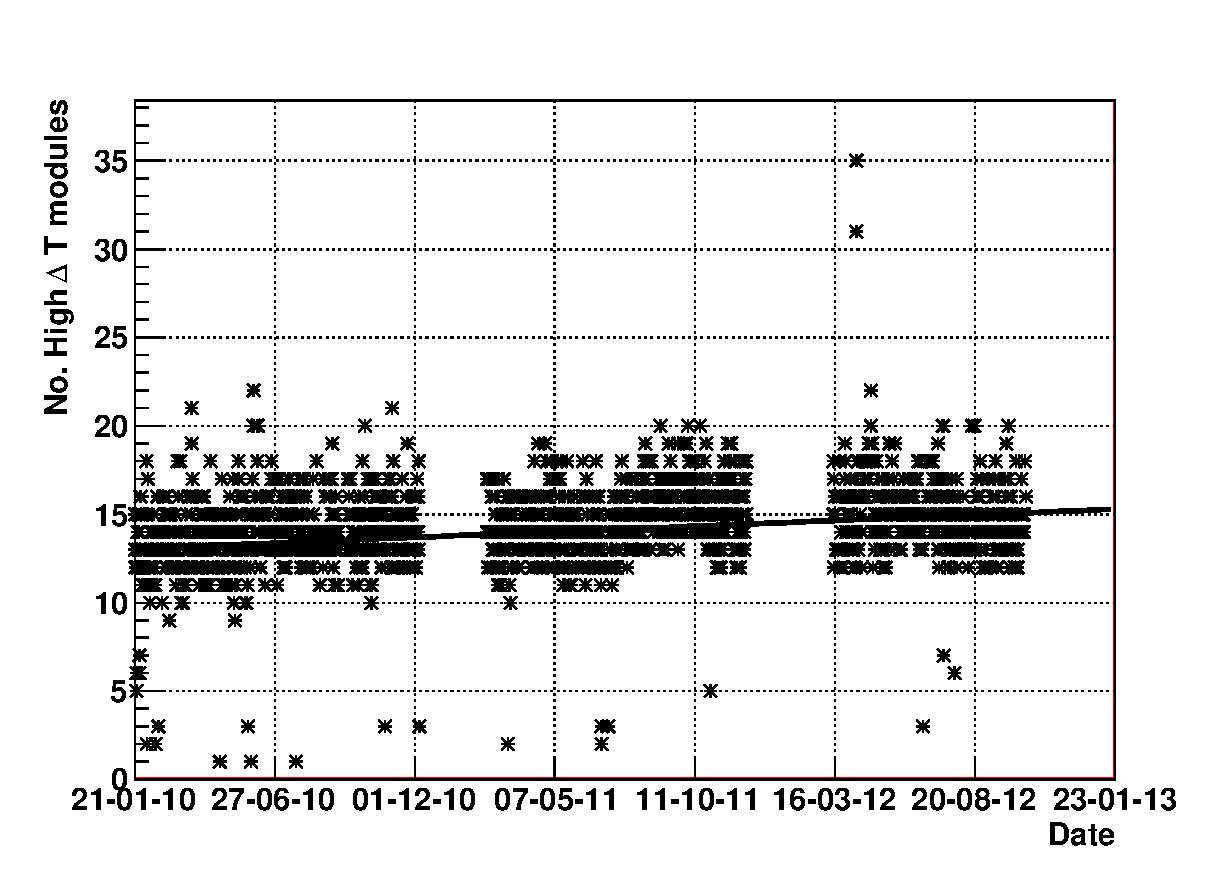
\includegraphics[width=0.47\textwidth]{number_problem_modules/num_high_delta_t}

	}
	\subfigure[]{
		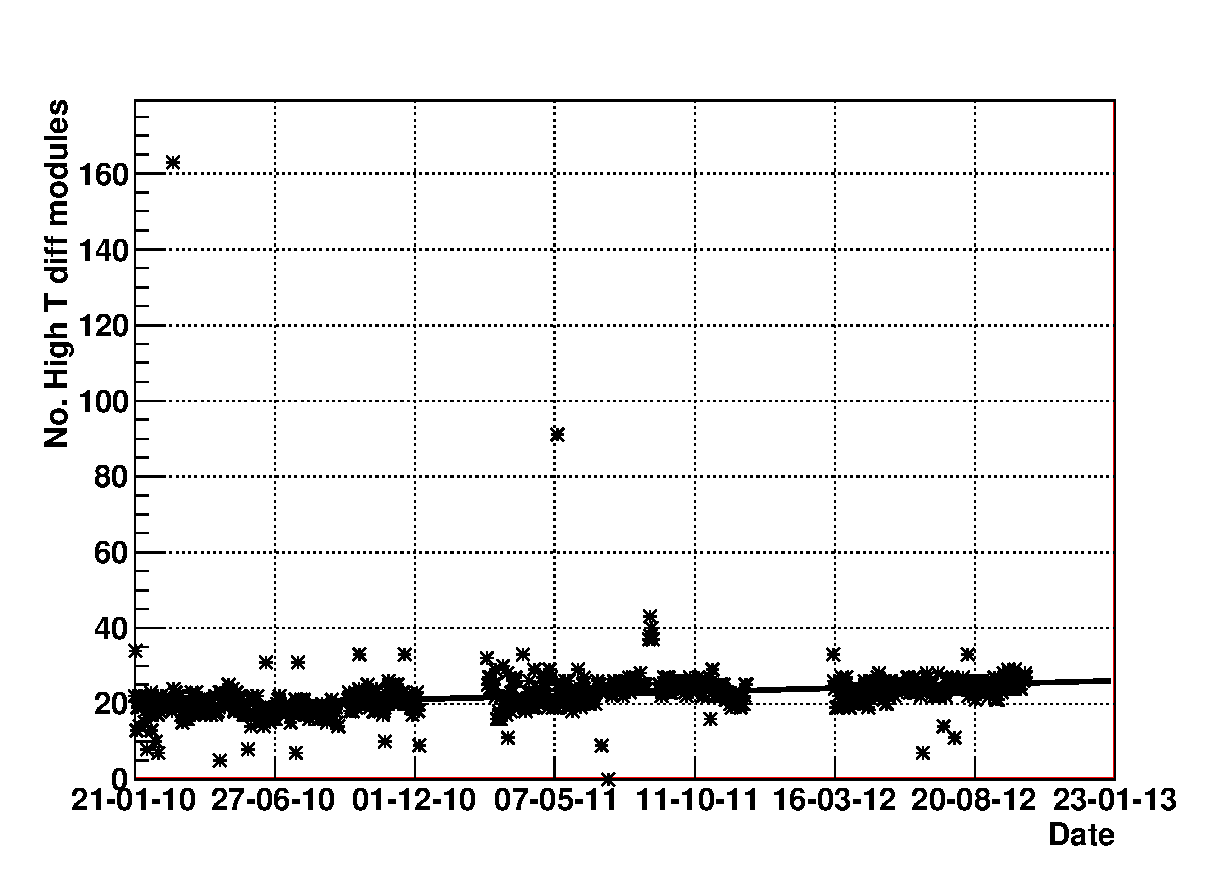
\includegraphics[width=0.47\textwidth]{number_problem_modules/num_high_t_diff}
	}
	\caption{The number of `problematic' modules with (a) \deltat and (b)
        \tdiff of greater magnitude than the problem threshold per day as a
        function of time between 20/01/2010 to 16/10/2012. The number of
        `problematic' modules is not seen to increase significantly as a
        function of time.}
	\label{fig:num_pm}
\end{figure}

\section{Behaviour of problematic modules}

For each of the problematic modules the value of the problematic monitoring variable has been plotted as a function of time for the first six months of 2010 in order to determine whether the problem is getting worse. For most of the problematic modules the magnitude of the monitoring variable does not increase over the period, aside from small fluctuations.  However, one module has been identified with a high \deltat of increasing magnitude, and four modules with a \tdiff of increasing magnitude. A further two show odd behavior. 

\begin{figure}[h]
 	\centering
	\subfigure[]{
		\includegraphics[width=0.47\textwidth]{pm_ev_dt_126-A5}
	}
	\subfigure[]{
		\includegraphics[width=0.47\textwidth]{pm_ev_dt_126-C6}
	}
	\caption{The temperature difference between the front and back of the module (\deltat) for barrel module Q3/B6/L126/I/P29/A5 (left) and barrel module Q3/B6/L126/O/P30/C6 (right) as a function of time between 20/1/2010 to 18/7/2010}
	\label{fig:pm_ev_dt}
\end{figure}

The plot on the left of~\ref{fig:pm_ev_dt} shows the only module with a \deltat of increasing magnitude. The temperature difference between the front and back of the module has increased by about 1.5$^\circ$C in six months, with back of the module warmer than the front. This suggests that the two sides of the module are slowly separating. The plot on the right of~\ref{fig:pm_ev_dt} shows a  module for which \deltat jumps between 0\dc  and 3-4\dc every 1 or 2 months. This suggests an intermittent failure in the integrity of the module, but is very unexpected behaviour and requires further investigation. No other problems with this module have been recorded.

Three modules were observed to have a \tdiff becoming more negative with time, indicating that they are becoming warmer relative to their neighbours by about 1\dc  over six months. This suggests a failure in coupling to the cooling pipe that is getting worse with time. One of these modules is shown on the left of Figure~\ref{fig:pm_ev_tdiff}.  The right hand plot of Figure~\ref{fig:pm_ev_tdiff} shows a module with \tdiff becoming more positive over time, and also showing sharp jumps in the variable. An increasing positive \tdiff means the module is cooler than its neighbours, and becoming even more cooler. This would suggest that the module is running at a lower power, although it is unclear why this would cause the \tdiff to increase over time, nor explain the sudden jumps. Generally modules running at lower power are detected with the DAQ (Data Acquisition) software, but no problem has been reported for this module. A further seven modules with a \tdiff which jumps between 0\dc and around +7 \dc have been observed.  All seven of these modules have other known problems; either the modules do not receive the high voltage, or there is a problem with the module communication. These modules are out of configuration, and data sent from these modules is not used for physics.

\begin{figure}[h]
 	\centering
	\subfigure[]{
		\includegraphics[width=0.47\textwidth]{pm_ev_tdiff_125-A4}
	}
	\subfigure[]{
		\includegraphics[width=0.47\textwidth]{pm_ev_tdiff_160-07}
	}
	\caption{The difference in temperature between the module and its neighbours (\tdiff) as a function of time for module Q2/B5/L102/I/P24/C3 (left) Q4/ECA/D4/L160/RO/07 (right) between 20/1/2010 to 18/7/2010. }
	\label{fig:pm_ev_tdiff}
\end{figure}

\section{Conclusions}

I plan to cross check problem modules against detector conditions and coincidences with events like powercuts, shutdowns, cooling failures etc, as well as studying characteristics of the individual modules such as the voltage arriving at the module. I also plan to cross check problematic modules against the `production database' which details tests made of modules at production to identify any correlations. 


\graphicspath{{Chapters/Reconstruction/Figures/}}
%\graphicspath{{Figures/}}
\label{chap:Reconstruction}
\chapter{Object Reconstruction}

In this chapter the software algorithms used to reconstruct and identify
different particles are described. Reconstruction involves reconstructing tracks in the
Inner Detector and Muon Spectrometer, identifying interaction vertices,
and identifying clusters of energy deposits in the calorimeter systems. These are
then combined to reconstruct particles such as electrons, muons, jets, photons,
tau leptons, as well as to measure properties as the event such as missing
transverse energy. 
Since triggering on electrons and muons is a crucial component of the
measurements described in this thesis, this is described in more detail here.

~\fig{particle-flow} shows schematically how different particles interect with
the different detector components. Muons leave a track in the Inner Detector,
typically deposit little in the calorimeters and then leave a track in the Muon
Spectrometer. Photons leave no track in the inner detector, and will typically
deposit all of their energy in the EM calorimeter, leaving an electromagtic
shower. Electrons also typically deposit all of their energy in the EM
calorimeter, but will also leave a track in the Inner Detector.
Charged hadrons such as protons leave a track in the Inner Detector, 
deposit minimal amounts of energy in the EM calorimeter, but then deposit
most of their energy in the hadronic calorimeter, leaving a long wide shower.
Neutral hadrons such as neutrons behave in a similar manner to charged hadrons,
but do not leave an Inner Detctor track. Neutrinos completely escape the
detector leaving no trace in any of the detectors systems.

\begin{figure}[h]
\centering
            \includegraphics[width=0.95\textwidth]{{ParticleFlow}.jpg}
\caption{
Schematic view of particles progression through the ATLAS detector. Figure from~\cite{ATLASPhotoGallery}.}
\label{fig:particle-flow}
\end{figure}

\section{Tracking}
\label{sec:reco-tracking}
\input{Tracking}

\section{Vertex Finding}
\label{sec:reco-vertexing}
Location of interaction vertices is an important ingredient to precision
particle-physics measurements. It is important to know which particles were
associated with the primary interaction vertex, and parameters such as the
longitudinal and transverse impact parameters can be used to distinguish signal
leptons from fakes, leptons from conversions, or secondary decays in jets.

In the ATLAS reconstruction process, vertex-finding occurs after reconstruction of
Inner Detector tracks, as described in \sec{reco-tracking}. The
vertex-finding algorithm must associate tracks with primary vertices, and obtain
a best fit for the vertex position and its uncertainty. Two approaches are
used in ATLAS for associating tracks with vertices~\cite{1742-6596-119-3-032033}. 

In `finding-after-fitting',
tracks are preselected by requiring that they are consistent with the collision
region. The tracks are ordered by their longitudinal impact parameter, and a
sliding window algorithm is used to identify clusters of tracks. A fit is 
carried out to obtain the vertex position. Outlier tracks are then removed if
they have a \chisquared\ with a probability of being consistent with the vertex
of less than 8\%. The vertex is the refitted, and the process iterates until
there are no outliers left, or the cluster becomes too small. In this procedure
the maximum number of vertices produced is determined at the clustering stage, and
once discarded, outlier tracks are not used again. This can be sub-optimal in
busy environments if the initial seeding does not correctly identify clusters.

An alternative approach, with better handling of outliers, is
`finding-through-fitting'. This is the default approach in ATLAS. Tracks are
again preselected by consistency with the interaction region, but in this case a
single seed vertex is formed out of all the preselected tracks. This is fitted, and
tracks identified as outliers in the fit are used to create a second vertex
seed. A simultaneous fit is then carried out of the two vertices, and again
outlier tracks are used to create a new primary vertex. The procedure is
iterated until none of the remaining outliers fit with any vertex with a
\chisquared\ probability of more than 1\%.

An `Adaptive Vertex Finding'~\cite{0954-3899-34-12-N01} algorithm is used in
both cases for the vertex position fitting. 
This uses a Kalman filter to minimise the least squares distances of the tracks from
the vertex position. After a preliminary fit, tracks are assigned a
weight depending on their compatibility with the vertex, with outlier tracks
being down-weighted so as to have less of a pull on the vertex position. The
process is iterated until convergence.


\section{Electron Reconstruction and Identification}
\label{sec:reco-el}
\subsection{Trigger}
\label{sec:reco-el-triggers}

Events containing electrons are triggered on using ATLAS's three level trigger
system as described in~\sec{detector-trigger}. They are triggered on at L1 by
requiring two adjacent towers of calorimeter cells of size
\deltaetadeltaphi{0.1}{0.1} have an energy above a certain threshold. The towers
are used to identify a RoI for use at L2. At L2 fast calorimeter and tracking
algorithms are used. The calorimeter clustering uses a similar algorithm to in
the offline reconstruction as described in~\sec{reco-el-reco}, except that the
highest \et\ cell in the middle calorimeter layer of the RoI is used as a seed
rather than using a sliding window algorithm. Basic shower shape cuts on
the width of the shower in $\eta$ and the ratio of energy deposits in the
different calorimeter layers are
used to reject backgrounds. The EF uses the offline reconstruction and
identification algorithms described in~\sec{reco-el-reco}
and~\sec{reco-el-id}, although slightly looser cuts are applied to remain fully
efficient offline. 
%It uses some information from just outside the RoI.

The bandwidth dedicated to electron and photon triggers is approximately 30\% of the
total EF bandwidth. As instantaneous luminosity increased throughout 2011 and
2012 it was necessary to regularly tighten the triggers to keep the bandwidth at
an acceptable level~\cite{Monticelli:1450947}. At the start of 2011 the primary single electron trigger
has a threshold of 20 \gev. When the instantaneous luminosity exceeded
2\timestenpower{33}~\instlumiunit\ the threshold was increased to 22 \gev, and as
the luminosity further increased to 3\timestenpower{33}~\instlumiunit, the identification
requirements used at L2 and EF were tightened. The L1 thresholds were also
brought closer to the EF threshold, and varying L1 thresholds with $\eta$ were
introduced to account for varying material before the calorimeter. A hadronic
leakage cut was also introduced to further reduce the L1 rate. In 2012 the
threshold was further raised to 24 \gev, and a track isolation cut introduced at
EF, requiring that the total \pt\ of tracks surrounding the
electron's track in a cone of \deltaRlt{0.2} to have less than 10\% of the \pt\ of
the electron.

\subsection{Reconstruction}
\label{sec:reco-el-reco}

Electrons are reconstructed in the central region (\modetalt{2.5}) by searching
for EM calorimeter clusters and matching them to Inner Detector
tracks~\cite{ATL-PHYS-PUB-2011-006,Aad:2011mk}; this is
referred to as the \intro{standard} electron algorithm and is described below.
In the forward regions (\modetabetween{2.5}{4.9}) there is no Inner Detector
tracking, and electrons are reconstructed solely from calorimeter clusters; this
is also described below. The standard algorithm drops in efficiency at very
low \pt\
(a few \gev), but an alternative \intro{soft-e} algorithm can be used to recover
efficiency. This uses Inner Detector tracks as seeds, which it extrapolates into
the EM calorimeter and attempts to build clusters. It is not used in
this thesis so is not described in detail here.

\subsubsection{Standard Electron Reconstruction}

Reconstruction begins
with the construction of seed clusters in the EM calorimeter. These are formed from
calorimeter towers of size \deltaetadeltaphi{0.025}{0.025}, corresponding to the
size of cells in the second layer of the EM calorimeter. This
results in a grid of $200 \times 256$ towers. The energy
of the tower is the sum of the cells in all three layers
falling within the tower. Where cells are shared between more than one tower, the
energy is shared according the fractional overlap of the cell with each
tower. The seed cells are formed by sliding a
window of size \deltaetadeltaphi{0.075}{0.125} ($3 \times 5$ towers) over the
grid of towers and identifying local maxima with \etgt{2.5}. The position
of the cluster is taken to be the energy weighted $\eta$, $\phi$ barycentre of
cells in a window around the centre of the cluster. If two seeds are closer than
\deltaetadeltaphi{0.050}{0.050} only the one with higher \et\ is kept.

Electron candidates are then formed by matching Inner Detector tracks to the
seed clusters. If there is a reasonable agreement ($\Delta \eta <0.2$ and
$\Delta \phi <0.1$) between a track's co-ordinates (measured at the origin of the
track) and a cluster seed, the track is extrapolated from its last measurement point to
the middle layer of the EM calorimeter (TRT-only tracks are automatically
extrapolated). In $\eta$, the cluster is required to be within 
of$\Delta \eta <0.05$ of the track. In $\phi$, the cluster must be within $\Delta \phi < 0.1$ of
the track if it falls on the side towards which the track bends, or $\Delta
\phi < 0.05$ if it is on the opposite side. This asymmetry in the $\phi$
requirement is to
account for the fact that the electrons undergo heavy energy losses from
bremsstrahlung, due to the large amount of material in the Inner Detector, which
will tend to increase their bending,
particularly at high $\eta$. If a seed cluster matches to at least one track,
and electron candidate is formed. Seed clusters with no track matches are
considered as photon candidates. If several tracks match, tracks with hits with
silicon hits are preferred, and the one closest to the cluster in \deltaR\ 
is chosen. In the case of TRT-only tracks, only a matching in $\phi$ is required, 
due to the limited $\eta$ resolution in the TRT.

The clusters for electron candidates are then rebuilt, using a fixed rectangle of size 
\deltaetadeltaphi{0.075}{0.175} ($0.125 \times 0.125$) in the barrel (endcap),
again using a sliding window to find the local maximum. The cluster energy is
the sum of four components: the estimated energy deposits before the
calorimeter, the measured energy in the cluster, the estimated leakage laterally
into other calorimeter cells and the estimated longitudinal leakage behind the
EM calorimeter. The four terms are parameterised as a function of the measured
cluster energy in the pre-sampler (where it exists) and the measured energy in each of the three
calorimeter layers, based on detailed simulations of energy depositions in the
calorimeters and the dead material. At this stage additional calibrations are
applied to the electron energy based on measurements of \Zee\ and
\JPsiee~\cite{Aad:2011mk}. The energy of the electron is taken as the cluster
energy, and the direction as the track $\eta$ and $\phi$, providing the track
has sufficient silicon hits.

\subsubsection{Forward Electron Reconstruction}

Forward electrons are reconstructed from energy deposits in the calorimeter
only. \intro{Topological clusters}~\cite{Lampl:1099735} are formed by grouping neighbouring cells in three
dimensions. The topological clusters do not have a fixed size, but will depend
on the energy deposit and the clustering criteria used. Cells with a
signal versus noise significance above a high threshold $t_{\rm{seed}}$ are used as seeds.
Neighbouring cells with a signal significance above a lower threshold
$t_{\rm{cell}}$ are added to the cluster. The neighbours may act as
secondary seeds if they have signal significance above an intermediate threshold
$t_{\rm{neighbour}}$. For electron topological clusters $t_{\rm{seed}}$ is set
equal to $t_{\rm{neighbour}}$. The lower threshold at the cell perimeter ensures that
tails of showers are not discarded, while the higher thresholds for seeds and
neighbors suppress electronics and pile-up noise. The cells are split if they
contain more than one local maxima above a certain energy threshold. 

An electron candidate is constructed if the cluster has \etgt{5} and only a
small hadronic energy component. The energy
of the electron is taken as the sum of the energy of all cells belonging to the cluster,
corrected for energy loss before the calorimeter and lateral and for longitudinal
leakages. The direction of the forward electron is taken as the barycentre of the cells
belonging to the cluster.

\subsubsection{Improvements to electron reconstruction in 2011 and 2012}

By default the ATLAS track fitting assumes a pion hypothesis for the modelling
of material effects, as described in~\sec{tracking-std}. This does not account well for energy losses via
bremsstrahlung. Due to their small mass, these losses are most substantial for
electrons, and can have significant effects on their trajectories through the magnetic
field. The amount of material in the Inner Detector in terms of radiation lengths
$X_{0}$ is shown in~\fig{id-material}. The material budget in the Inner detector
is highly non uniform with, high concentration of material at high $\eta$ and at certain radii.
This leads to large variations of the reconstruction efficiency as a function of
$\eta$, and degradations in estimates of the track parameters. To this end the
deault ATLAS reconstruction was progressively improved in 2011 and 2012 to
better account for energy losses due to \brem\ in the Inner Detector.

\begin{figure}[h]
\centering
            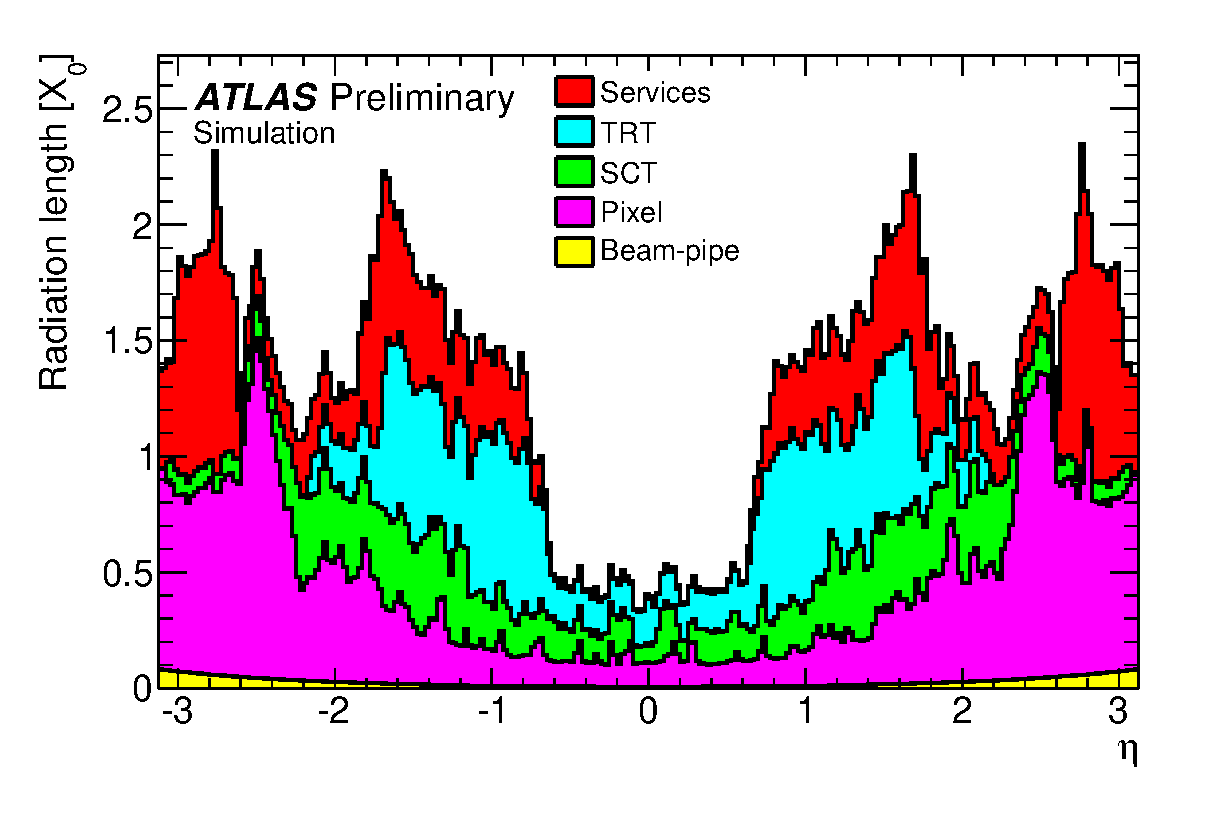
\includegraphics[width=0.8\textwidth]{id_material}
\caption{
Distribution of the Inner Detector material for each sub-detector as a
function of the pseudorapidity. The material of the Pixel and SCT detectors
includes passive material arising from electronics, cabling, cooling and
mechanical support. Figure from~\cite{ATLAS-CONF-2012-047}.}
\label{fig:id-material}
\end{figure}


The radiative loss of energy via \brem\ is highly non-Gaussian, and so is not
well modelled by the standard Kalman Filter, which can only incorporate Gaussian
noise terms. A non-linear extension of the
Kalman filter, the {\it Gaussian Sum Filter (GSF)}, has been
developed~\cite{Fruhwirth2003131,Atkinson:1448253}. It
approximates the PDF for energy loss from \brem\ as a weighted sum of Gaussian
components, and uses a separate Kalman Filter to process each one. For example,
one can consider the extrapolation of a measurement from a surface $k-1$ with state
described by $n_{k-1}$ components to surface $k$, where $\epsilon_{k}$ Gaussians
are used to describe the energy losses due to \brem\ between surfaces $k-1$ and
$k$. A separate Kalman Filter is applied to each of the $n_{k-1}$
components, for each of the $\epsilon_{k}$ noise terms, resulting in the state at
surface $k$ being described by $n_{k} = n_{k-1} \cdot \epsilon_{k}$ components.
At each layer the number of components is artificially reduced to a fixed number
by merging similar components,
in order to make the extrapolation computationally feasible.
Using the GSF filter allows for better pattern recognition by picking up hits
occurring after kinks in tracks caused by \brem, as well as improving the
resolution of the track parameters.

%\subsubsection{2011 Improvements}

For 2011 data taking, `brem-refitting' was applied to
reconstructed electron candidates~\cite{ATLAS-CONF-2012-047}. For technical reasons, it was not possible to
include the \brem\ recovery from the beginning of electron reconstruction.
Instead, electrons were reconstructed using the standard pion hypothesis
tracking and track cluster matching as described above. The tracks of these candidates were then refitted
using the GSF algorithm. All tracks with \ptgtMeV{400} and \modetalt{2.5} assigned to
electron candidates were refitted, the cluster-track matching re-run
using the collection of refitted tracks, and the rest of the electron reconstruction
chain re-run using these refitted candidates. This led to the best matches between
cluster and track changing in approximately 5\% of cases at high pseudo-rapidity (0.8 \%
overall). However, since it was only possible to run the refitting on tracks
already associated to electron clusters using the standard tracking, the full
benefit of using GSF was not gained as many tracks with significant energy loss
from \brem\ would not be reconstructed successfully by the standard tracking and
thus could not be re-fitted. For this reason the brem-refitting did not
significantly improve the reconstruction efficiency, but did significantly
improve the resolution of track parameters in the bending plane such as \dzero, \dzerosig,
$\phi$ and \qoverp. For example, \fig{d0Sig-gsf} shows the impact parameter
significance (\dzerosig) distribution with and without the GSF refit. 

\begin{figure}[h!]
\centering
            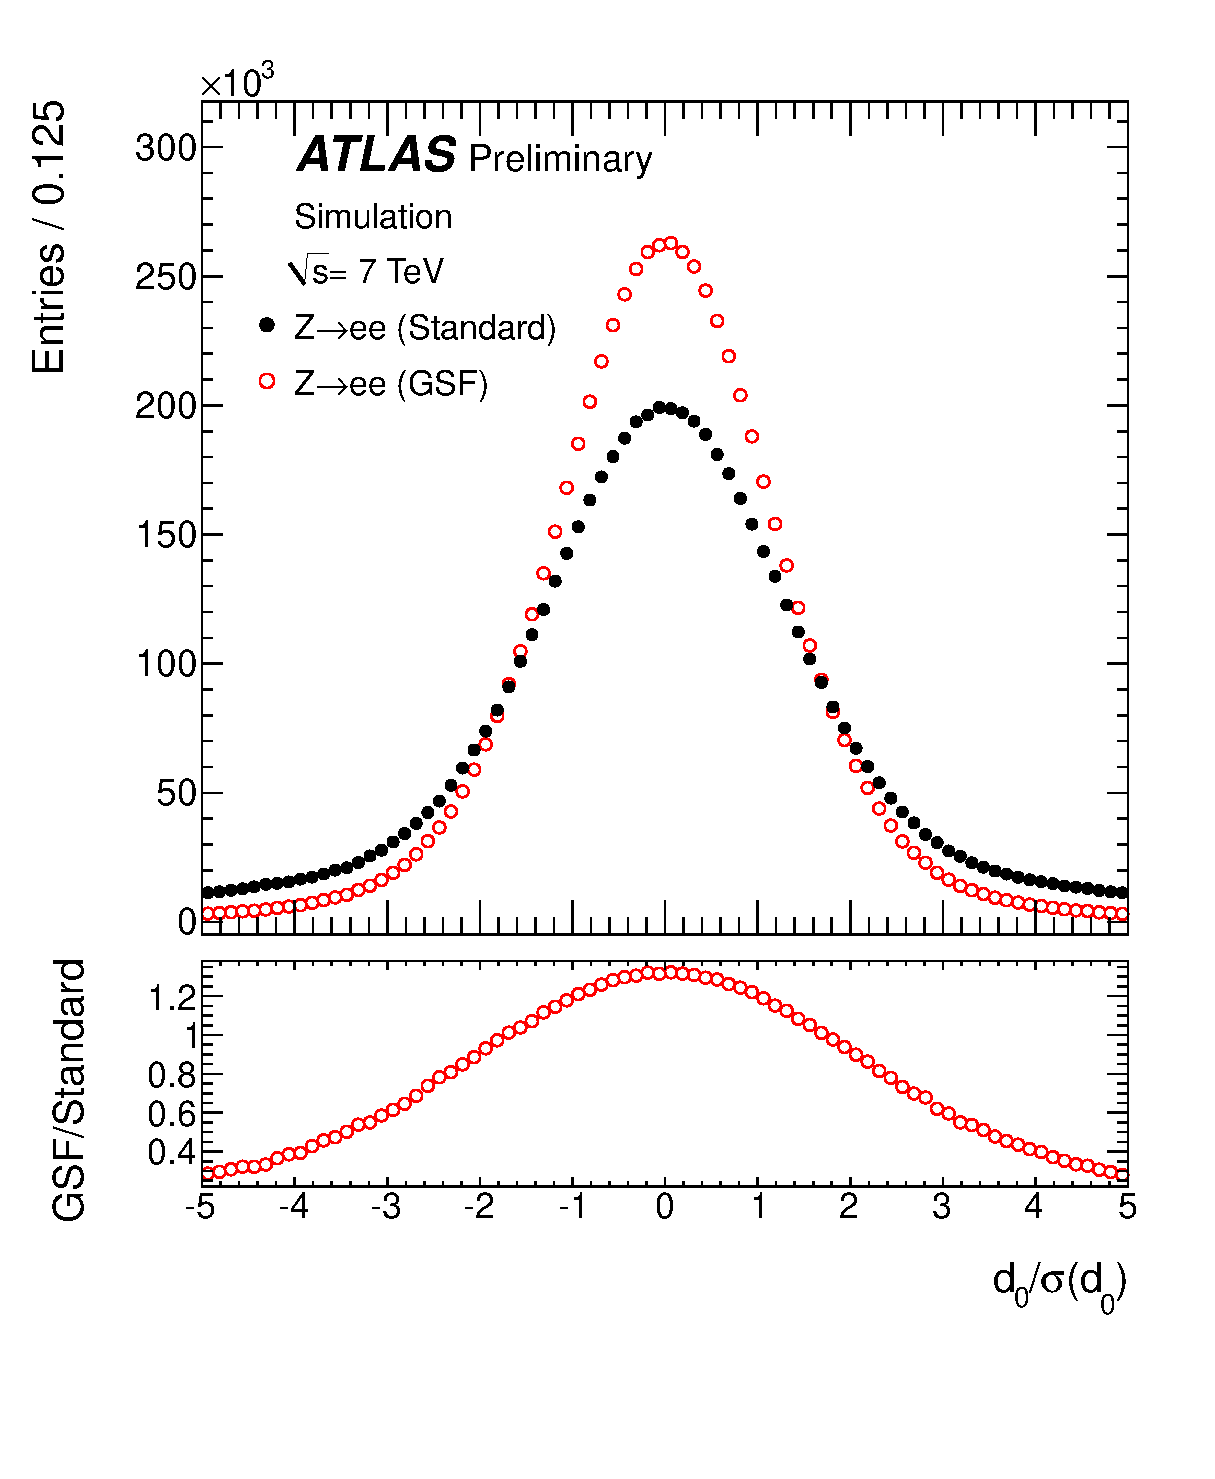
\includegraphics[width=0.7\textwidth]{d0Sig_gsf}
\caption{
Distribution of the simulated transverse impact parameter significance for GSF (open
red) and standard (solid black) electrons from \Z-boson decays. 
%The bottom plots show the ratio of the entries of the GSF and standard
%electrons per bin
Figure from~\cite{ATLAS-CONF-2012-047}.}
\label{fig:d0Sig-gsf}
\end{figure}

%\subsubsection{2012 Improvements}

In 2012, improvements were made to all stages of the electron reconstruction
chain, from the initial tracking pattern recognition through to the track
cluster matching~\cite{HSG2:1456228}. 

Since the GSF tracking takes approximately 10 times more time to
run than the standard Kalman filter, it is not feasible to fit all tracks using
the GSF when doing the initial pattern recognition and track finding (see~\sec{tracking-std}). 
Additionally, the use of such a filter with electron hypothesis would
negatively affect non-electron tracks. Instead, the effects of \brem\ on
electron tracks are crudely modelled at the initial pattern recognition by allowing for 30\% energy loss at each surface for tracks with
momentum above 1 \gev. In order to avoid degrading non-electron tracks, this allowance is only made in regions of interest in a
cone of \deltaRlt{0.3} around EM calorimeter clusters. 

The global \chisquared\
fitter was also improved to allow for electron hypothesis tracks. Tracks
rejected due to low \chisquared\ at the ambiguity resolution stage in a RoI were
refitted using a modified `electron hypothesis' global \chisquared\ fitter. This
attempts to find the layer with the most significant \brem\ energy loss, then
reruns the fit with only an energy loss term for the most significant \brem\
loss. The advantage of this over the standard \chisquared\ fit, which allows
includes an energy loss term for each layer, is that in the latter approach the
electron momentum tends to be overestimated as all of the energy loss terms tend
to take the average energy loss value, rather than correctly identifying one layer with large
energy loss. The modified \chisquared\ fitter gives a significant improvement in the track
parameter resolution, giving an improvement almost as great as using the more
sophisticated GSF algorithm, but running in approximately one tenth of the time.

At this stage, there will still be a number of tracks which had large energy
losses from \brem\ and were consequentially badly fitted. A refit using the GSF
fitter described above is thus carried out for all tracks loosely matched to an
EM calorimeter cluster. Two forms are matching are carried out: the first
(\deltaR) between the
track parameters extrapolated to the second layer of the calorimeter and the
barycentre of the calorimeter cluster, and the second (\deltaR$^{\rm{rescaled}}$) where the track momentum is
scaled to the cluster energy before extrapolating the track to the calorimeter.
Loose cuts are made on \deltaR\ and \deltaR$^{\rm{rescaled}}$, with the cuts on
\deltaR$^{\rm{rescaled}}$ being slightly tighter.
Tracks which match under either of the two scenarios are refitted; the latter
category aims to select tracks with low momentum that have suffered large
\brem\ and would otherwise be missed. The final matching of the refitted tracks
to the clusters and selection of the best match is also improved; again both the
original \deltaR\ and the \deltaR$^{\rm{rescaled}}$ after scaling the track
momentum to the cluster
energy are computed. Tracks with Pixel detector hits are preferred. If there are
more than two tracks with Pixel hits the one with the smaller
\deltaR$^{\rm{rescaled}}$ is preferred, providing they are well enough
separated in \deltaR$^{\rm{rescaled}}$, otherwise the one with smaller \deltaR\
is chosen.

Overall these improvements increase the electron reconstruction efficiency by
$\sim1\%$ in the calorimeter barrel and $\sim5\%$ in the calorimeter endcaps.
For low \et\ electrons (\etlt{20}) the improvement is up to 8\%.

\subsubsection{Electron Reconstruction Efficiencies}

\begin{figure}[h]
\centering
	\subfigure[]{
            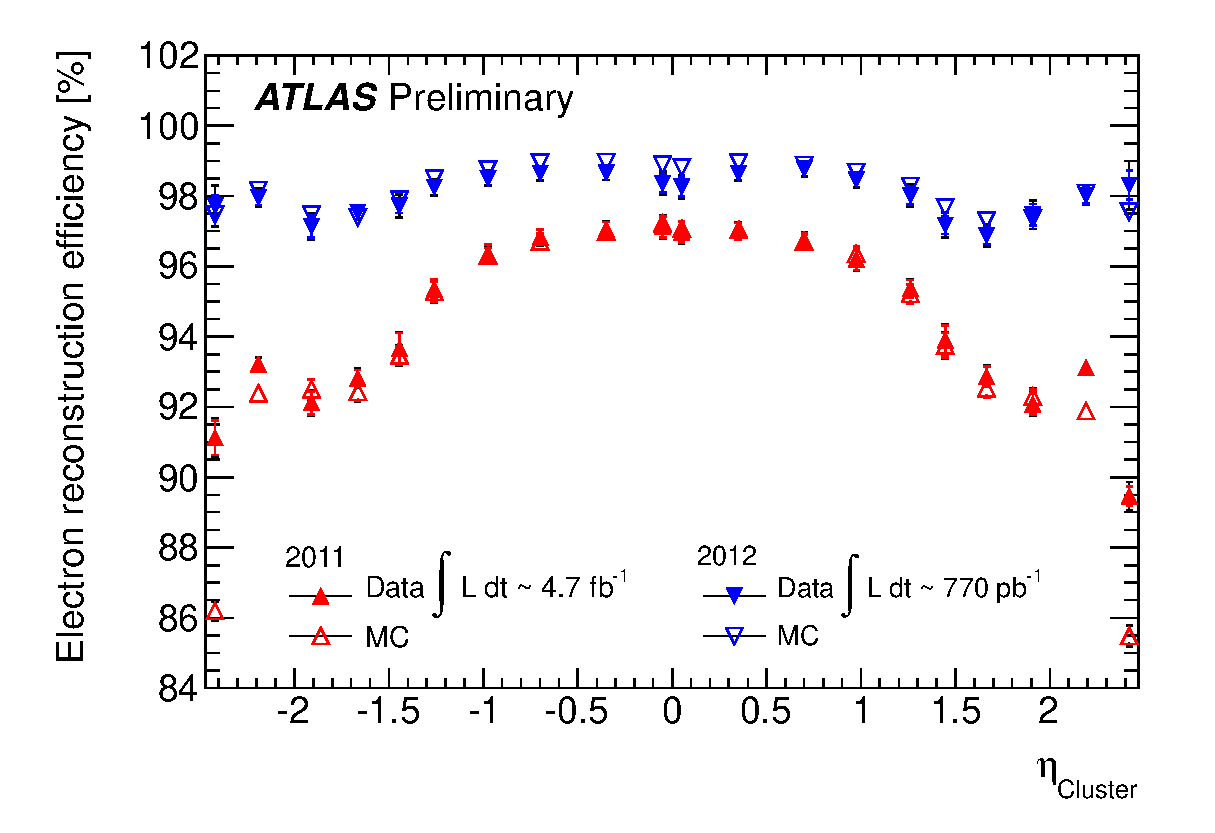
\includegraphics[width=0.47\textwidth]{ElRecoEffEtaBin2011_2012}
        }
	\subfigure[]{
            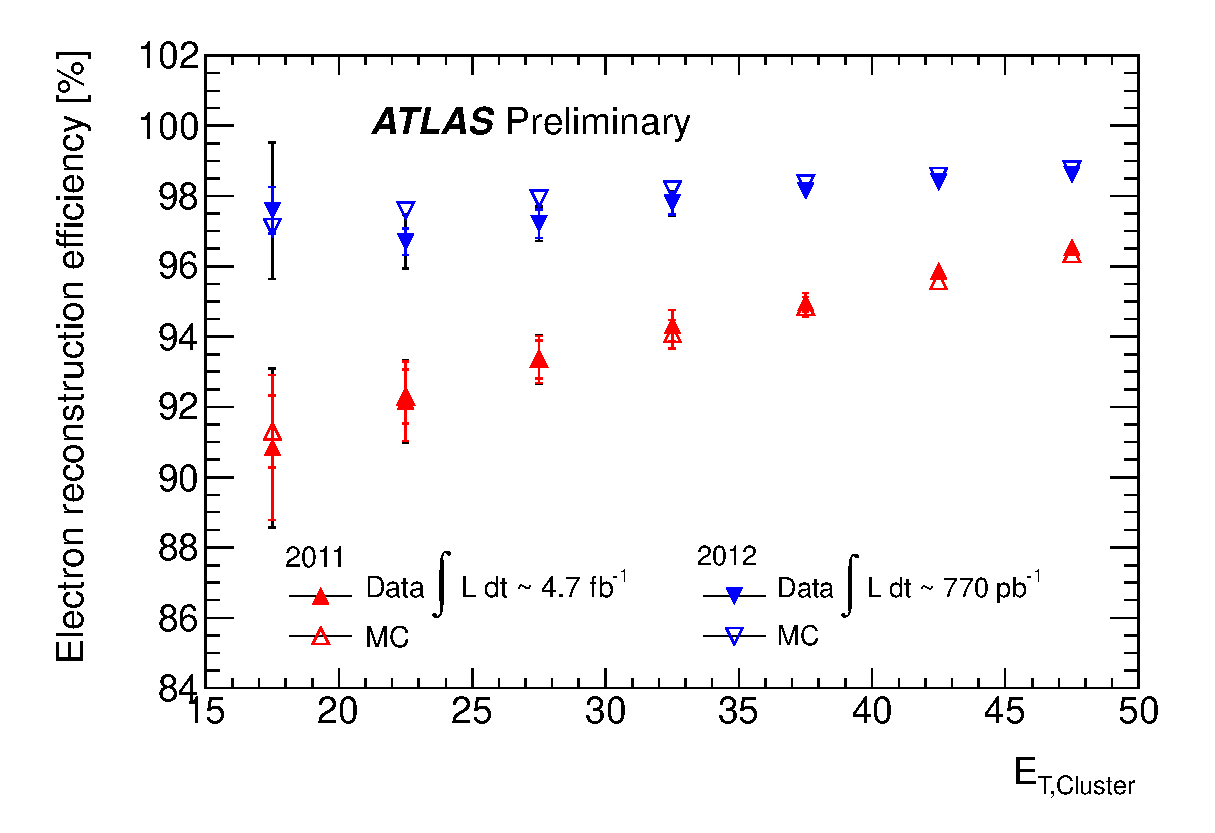
\includegraphics[width=0.47\textwidth]{ElRecoEffPtBin2011_2012}
        }
\caption{Electron reconstruction efficiency in 2011 and 2012 as a function of (a) the cluster
$\eta$ and (b) the cluster \et. The solid coloured points show the efficiency
observed in data whilst the open points show the simulated efficiency in
Monte-Carlo. Figures from~\cite{ElectronEfficiency2012}.}
\label{fig:el-reco-eff}
\end{figure}

\subsection{Identification}
\label{sec:reco-el-id}

The electron candidates reconstructed as described in the previous section will
contain a high contamination from jets faking electrons, non-isolated electrons
from decays in jets and electrons from photon conversions. In order to identify prompt isolated photons a
cut based identification is used. Cuts are made on variables relating to the
shape of the electromagnetic shower in the calorimeter, the quality of the Inner Detector track, the
track-calorimeter matching and particle identification information from the
TRT. The cuts were optimised using a multivariate analysis program (TMVA), in 10 bins
of cluster $\eta$ and 11 bins of cluster \et\ from 5 \gev\ to $>80$ \gev.
Three reference sets of cuts are used, denoted \loose, \medium\ and \tight,
designed to give progressively greater background rejection, at the cost of
signal efficiency. The expected jet rejections (from simulation) of the three points are 500, 5000
and 50000 respectively~\cite{ATL-PHYS-PUB-2011-006}.

In order to maintain manageable trigger rates with increased instantaneous
luminosity, the original \loose, \medium\ and \tight\ were re-optimised in order
to increase background rejection. The new working points are denoted \loosePP,
\mediumPP\ and \tightPP. In 2012, the identification was further re-optimised to
prevent drops in efficiency in events with high pileup of up to 20\%. 

In both 2011 and 2012 \loosePP\ cuts on shower shape variables in the first and
second layers of the EM calorimeter, leakage into the hadronic
calorimeter, track quality in the silicon detectors and loose track cluster
matching. The variables cut on are as follows:

\subsubsection{\loosePP\ Requirements}

\begin{itemize}

    \item {\bf Shower Shapes:} cuts are made on the following shower shape
    variables:

    \begin{itemize}
        \item Hadronic leakage, \Rhad, the ratio of \et\ in the first layer of
        the hadronic calorimeter to the \et\ of the EM cluster. In the range
        \modetabetween{0.8}{1.37} the \et\ of the full hadronic calorimeter is
        used, to compensate for the crack between the barrel and extended barrel
        of the tile calorimeter.
        \item Lateral width of the shower in the second layer of the EM
        calorimeter, \wetatwo.
        \item Ratio of the energy difference between with the largest and second
        largest energy deposit in the first layer of the EM calorimeter over the
        sum of their energies, \Eratio.
        \item Total width of the shower in the first layer of the EM
        calorimeter, \wstot.
    \end{itemize}

    \item {\bf Silicon Hits:} at least 7 hits in the silicon detectors, of which at
    least one must be in the pixel detector. This ensures good track quality and
    rejects backgrounds from conversions or Dalitz-decays.
    \item {\bf Track-Cluster matching:} a loose matching in $\eta$ is applied,
    requiring \deltaetalt{0.015}
\end{itemize}

The shower shape variables \Reta\ and \Rhad\ are particularly susceptible to
pileup since they sample a large area of the calorimeter. Cuts on these
variables were therefore
loosened in 2011 with respect to 2012, reducing the rejection power of \loosePP\
by about 20\%.

\subsubsection{\mediumPP\ Requirements}

All \loosePP\ cuts are required to be passed, and in addition:

\begin{itemize}
    \item {\bf Shower Shapes:} the shower shape cuts made in \loosePP
    (\Reta, \Rhad, \wetatwo, \Eratio, \wstot) are made at tighter values. For
    2012, the cuts on \Reta\ and \Rhad\ were loosened with respect to 2011, and
    made at the same value as for \loosePP, whilst the cuts on  \wetatwo, \Eratio\ and
    \wstot\ were tightened with respect to 2011.

    \item {\bf Track-Cluster matching:} a tighter matching in $\eta$ is applied,
    requiring \deltaetalt{0.005}.

    \item {\bf Impact Parameter:} require that the electron's track has a
    transverse impact parameter \dzero $<$ 5 mm.

    \item {\bf Silicon Hits:} stricter requirements are made on hits in the
    silicon detectors. Require that there is at least one hit in the b-layer for
    \modetalt{2.01} (\modetalt{2.37} in 2012). In 2011, at least 1
    Pixel hit is required for \modetalt{2.01} and at least two for
    \modetagt{2.01}. For 2012, two Pixel hits are required in all bins.

    \item {\bf Fraction in third calorimeter layer \fthree:} for 2012 a cut on the
    fraction of the shower energy deposited in the third layer of the EM
    calorimeter was added to compensate for the loosening of the cuts in the
    first layer of the calorimeter. This cut is only applied for \etlt{80}, since
    the depth of the EM shower and hence leakage into the third layer increases
    with energy.

    \item {\bf TRT High Threshold Hits} A loose requirement is made on the
    fraction of high-threshold (HT) hits from transition radiation photons in the
    TRT detector (see~\sec{Detector-TRT}).

\end{itemize}

\subsubsection{\tightPP\ Requirements}


All \mediumPP\ cuts are required to be passed, and in addition:

\begin{itemize}
    \item {\bf Shower Shapes:} cuts on shower shape variables are made at equal
    or tighter values to those for \mediumPP. As for \mediumPP,
    the cuts on \Reta\ and \Rhad\ were loosened in 2012 with respect to 2011, 
    whilst the cuts on  \wetatwo, \Eratio\ and
    \wstot\ were tightened.

    \item {\bf Track-Cluster matching:} a cluster matching in $\phi$ is added,
    requiring \deltaphilt{0.02}, and cuts are made on the ratio of the cluster
    energy to the track momentum, \Eoverp.

    \item {\bf Impact Parameter:} the
    transverse impact parameter cut is tightened to \dzero\ $<$ 1 mm.

    \item {\bf Silicon Hits:} stricter requirements are made on hits in the
    silicon detectors, requiring that there is at least one hit in the b-layer for
    all $\eta$, and, in 2012, at least 2 hits in the Pixel detector for all
    $\eta$.

    \item {\bf Conversion Rejection:} candidates matched to reconstructed photon
    conversions are rejected.

\end{itemize}

\subsubsection{Forward Electron Identification}

Since in the forward region there is no tracking from the Inner Detector,
identification in the forward region must rely on calorimeter shower shape
variables alone. A god discrimination between electrons and hadrons may be made
due to the fine transverse and longitudinal segmentation of the calorimeter, but
it is not possible to distinguish electrons and photons in the forward regions.
Two reference sets of cuts are defined for forward electrons, \loose\ and
\tight.

\subsubsection{Forward \loose\ Requirements}

Cuts are made on the following variables:

\begin{itemize}
    \item {\bf Shower depth, $\lambda_{\rm centre}$} the distance of the shower
    barycentre from the front face of the calorimeter along its axis.  
    \item {\bf Longitudinal Second Moment, $\langle \lambda^2 \rangle$} the second
    moment\footnote{The $n^{\rm th}$ moment is defined as $\langle x^n \rangle =
    \frac{\sum_{i} E_i x^n_i}{\sum_{i} E_i}$ where $i$ runs over all cells in the
    cluster.} of the distance of each cell to
    the shower barycentre in the longitudinal direction.  
    \item {\bf Transverse Second Moment, $\langle r^2 \rangle$} the second moment of the 
    distance of each cell to the shower barycentre in the transverse direction.
\end{itemize}

\subsubsection{Forward \tight\ Requirements}

All of the \loose\ cuts are required to be passed, an in addition cuts are made
on the following variables:

\begin{itemize}
    \item {\bf Fraction Fraction of cluster energy in the most energetic cell,
    $f_{\rm max}$.}
    \item {\bf Normalized lateral moment, $\frac{w_{2}}{w_{2} + w_{\rm max}}$} where
    $w_{2}$ is the second moment of $r_{i}$ setting $r_{i} = 0$ for the two most
    energetic cells and $w_{\rm max}$ is the second moment of $r_{i}$ setting
    $r_{i} = 4$ cm for the two most energetic cells and $r_{i} = 0$ for the
    remaining cells.
    \item {\bf Normalized longitudinal moment, $\frac{l_{2}}{l_{2} + l_{\rm
    max}}$}
    where, similarly to the normalised longitudinal moment, 
    $l_{2}$ is the second moment of $\lambda_{i}$ setting $\lambda_{i} = 0$ for the two most
    energetic cells and $l_{\rm max}$ is the second moment of $\lambda_{i}$ setting
    $\lambda_{i} = 10$ cm for the two most energetic cells and $\lambda_{i} = 0$ for the
    remaining cells.
\end{itemize}

\subsubsection{Electron Reconstruction Efficiencies}

\begin{figure}[h]
\centering
	\subfigure[]{
            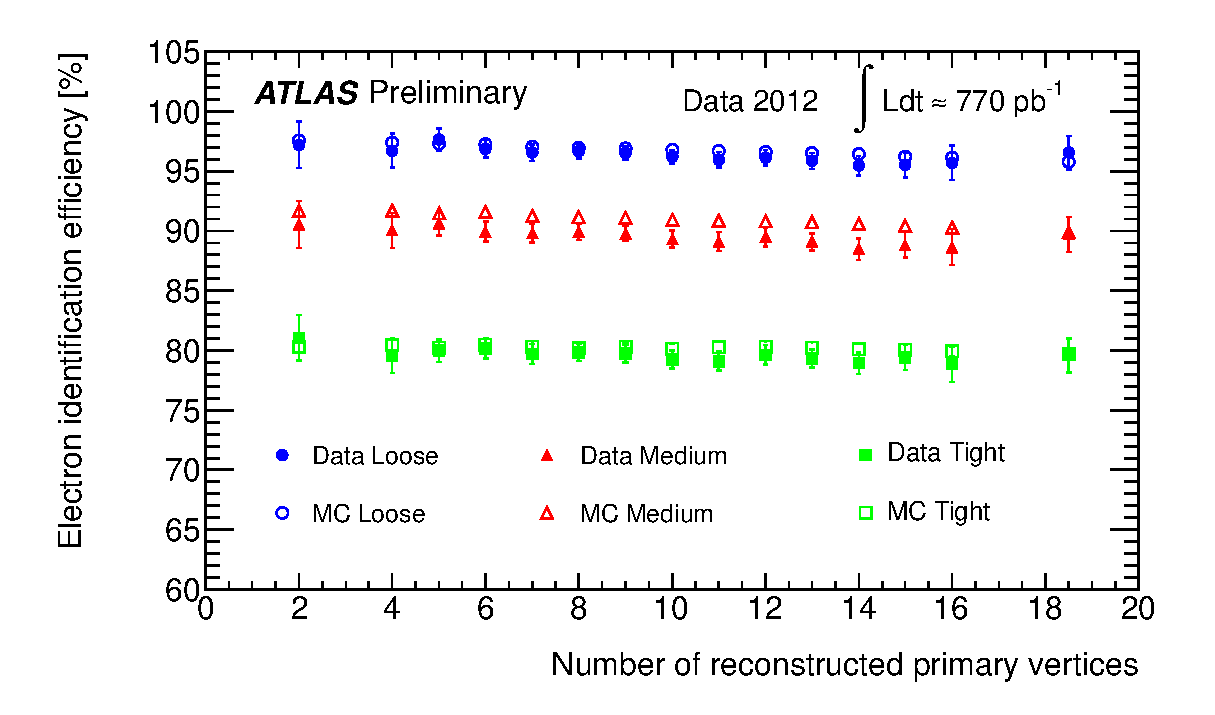
\includegraphics[width=0.47\textwidth]{ElIdEff_NPV_2012}
        }
	\subfigure[]{
            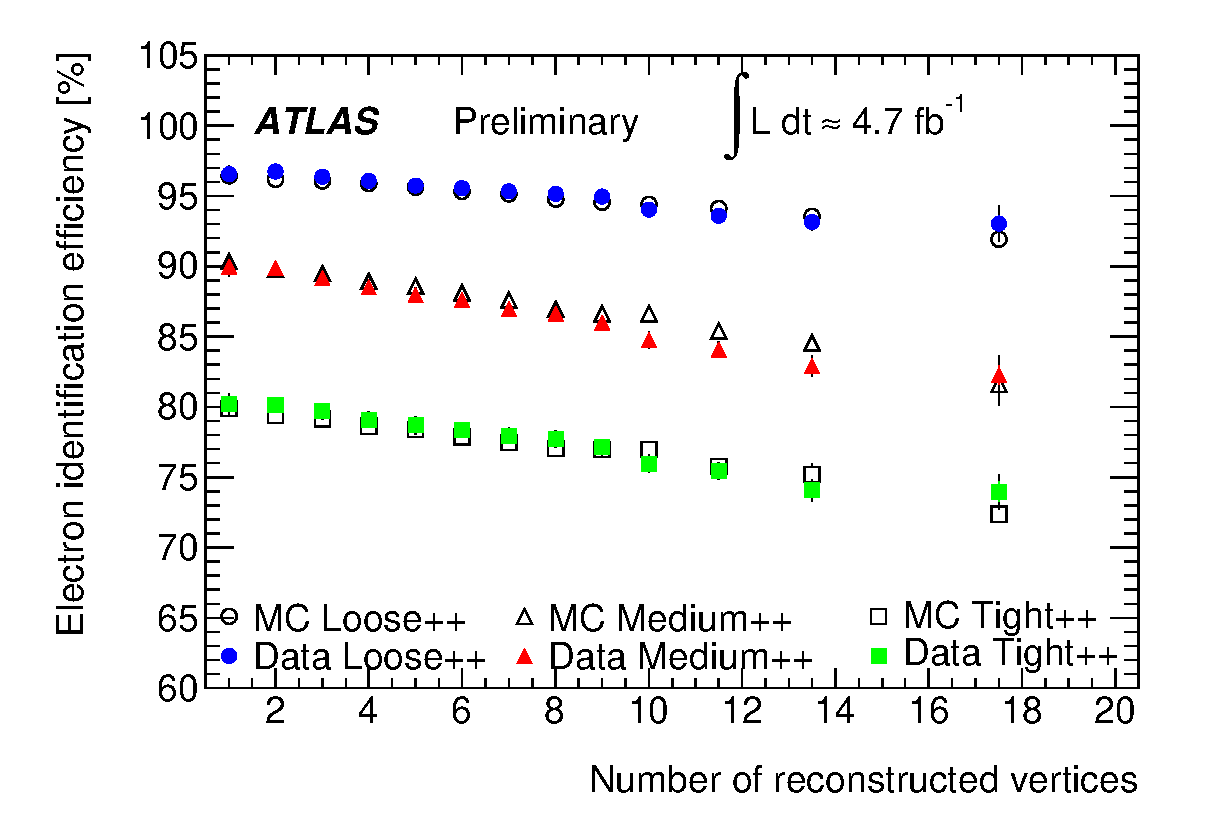
\includegraphics[width=0.47\textwidth]{Eff_PP_pileup2011}
        }
	\subfigure[]{
            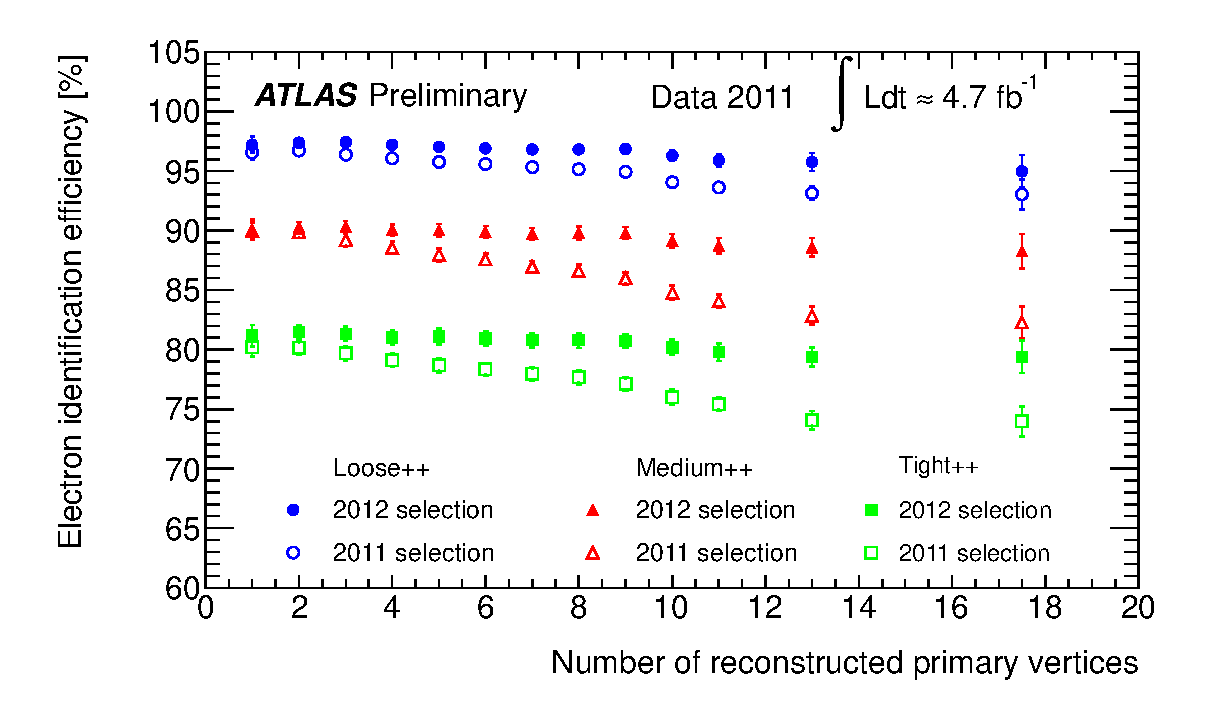
\includegraphics[width=0.47\textwidth]{data_effPP_vs_pvx_2011_2012}
        }
	\subfigure[]{
            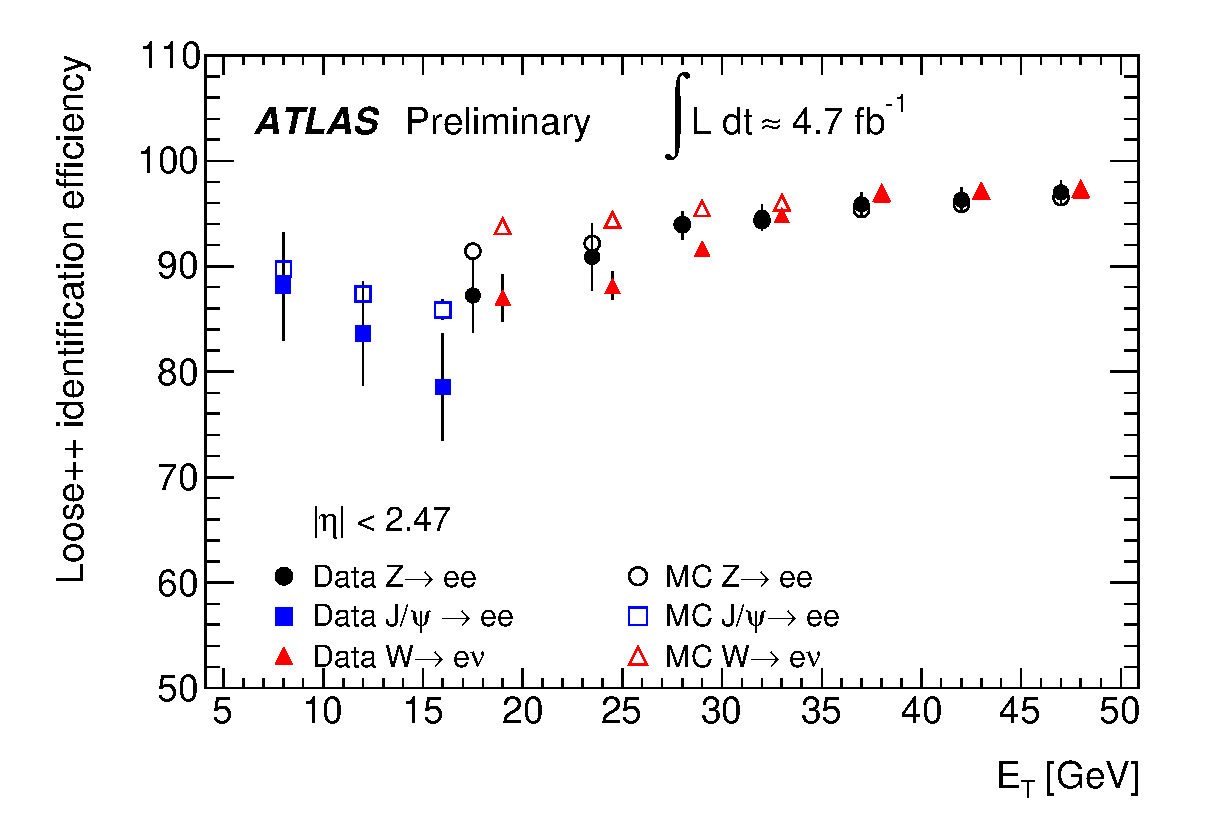
\includegraphics[width=0.47\textwidth]{ElLoosePPEfficiencyPt2011}
        }
\caption{Electron reconstruction efficiency in 2011 and 2012 as a function of (a) the cluster
$\eta$ and (b) the cluster \et. The solid coloured points show the efficiency
observed in data whilst the open points show the simulated efficiency in
Monte-Carlo. Figures
from~\cite{ElectronEfficiency2012,EfficiencyPileup,ElectronEfficiency2011,ElectronEffPV2011}.}
\label{fig:el-reco-eff}
\end{figure}


%The cluster reconstruction efficiency is very efficient for electrons:


\section{Muon Reconstruction and Identification}
\label{sec:reco-mu}
\subsection{Muon triggers}
\label{sec:reco-mu-triggers}

Muons are triggered on at L1 using the RPC in the barrel (\modetalt{1.05}) and
the TGC in the endcaps (\modetalt{2.4}). ~\fig{mu-trigger-diag} The chambers are arranged



\begin{figure}[h]
\centering
            \includegraphics[width=0.8\textwidth]{mu-trigger-diag}
\caption{
Distribution of the Inner Detector material for each sub-detector as a
function of the pseudorapidity. The material of the Pixel and SCT detectors
includes passive material arising from electronics, cabling, cooling and
mechanical support. Figure from~\cite{2012EPJC...72.1849A}.}
\label{fig:mu-trigger-diag}
\end{figure}

- Not affected significantly by pileup, but increased lumi requires tightening of pT selection in 2012.
   - 2011: 18 GeV threshold
   - 2012: 24 GeV, plus isolation: ptcone20/pt<12%. Tracks have to have z0<6mm
   


\subsection{Reconstruction and Identification}
\label{sec:reco-el-reco}


\section{Jet Reconstruction}
\label{sec:reco-jet}
Partons produced in particle interactions are not physically observable since
they hadronize and produce a collimated shower of particles known as a jet. In
order to reconstruct the jet in a physically meaningful way, it is necessary to
specify an algorithm to associate the multiple energy deposits in the calorimeters
to a single jet (\intro{clustering}) and a recombination scheme for how to combine their
four-momentum. The ATLAS hadronic calorimeters are non-compensating, so do not
compensate from energy lost from the hadronic shower due to production of
secondary particles such as neutrinos and muons that escape from the calorimeter
or due to leakage of the shower out of the calorimeter. It is thus necessary to
calibrate the response of the calorimeter to a hadronic shower.

Jet algorithms need to be theoretically well behaved with respect to QCD
divergences. In particular, it is important that the jets produced are not
affected by soft emissions (the algorithm must be \intro{collinear safe}) and
are not affected if a parton splits into two collinear partons (the algorithm
must be \intro{collinear safe}). Additionally, the algorithm must give the same
physics results regardless of whether the input is partons, particles (from
Monte-Carlo simulation) or calorimeter objects. There are two main classes of
jet clustering algorithm: cone algorithms and successive combination algorithms.
Cone algorithms start from seed objects and add in all other objects within a
cone of a specified size in $\Delta R$, where $\Delta R = \sqrt{(\Delta \eta)^{2} + (\Delta
\phi)^{2}} $. Cone algorithms are generally theoretically unsafe as soft or
collinear emissions can affect the choice of seeds. Successive combination
algorithms iteratively merge pairs of objects according to a definition of distance that
generally involves the distance between the objects and their transverse
momentum.

In ATLAS, the default jet clustering algorithm is a successive combination
algorithm called \antikt~\cite{1126-6708-2008-04-063}. This combines objects
according to the distance parameters $d_{i,j} =
{\rm min}(p_{T,i}^{-2},p_{T,j}^{-2}) \cdot \frac{ \Delta R }{R}$ and $d_{i,\rm{beam}} =
p_{T,i}^{-2}$ where $p_{T,i}$ is the transverse momentum of object $i$ and
$\Delta R$ is the distance between objects $i,j$ in $\eta, \phi$ as defined above.
The parameter $R$ is a parameter controlling the size of the jet, and is
analageous to the cone size in a cone based jet algorithm. The algorithm starts
with a list of all objects, and calculates $d_{i,j}$ for all pairs of objects and
$d_{i,{\rm beam}}$ for all objects. If the minimum of all $\{ d_{i,j}, d_{i,{\rm
beam}} \}$ is a  $d_{i,j}$ the objects will be merged; if it is a $ d_{i,{\rm
beam}}$ the object will be considered a jet and removed from the list. This
process is repeated until there are no object remaining. This algorithm is
collinear and infrared safe as soft radiation is clustered to harder objects. 
It results in regular conical jets, which is experimentally desirable
since it gives a well defined jet area that can be used for pileup supression.
Where jets are used in this thesis, the $R$ parameter is set to be 0.4.

The four momentum of the jet is obtained simply by summing the four-momentum of
the constituant objects. This scheme conserves energy and momentum, and allows a
meaningful definition for the jet mass.





\part{Analysis}
\graphicspath{{Chapters/ObjEventSelection/Figures/}}
\chapter{Object and Event Selection}
\label{chap:ObjEventSelection}

\section{Electron Selection}

Electron reconstruction and identification was described in~\sec{reco-el}. Both
central electrons with \modetalt{2.47} and forward electrons are used. In
addition to the indentification requirements described in~\sec{reco-el}
additional selection requirements are imposed to select electrons likely to have
originated from \Z\ boson decays and to reject backgrounds. The requirements are
slightly different for the 8 \tev\ analysis compared to the 7 \tev\ analysis,
reflecting the different experimental conditions (such as higher pile-up in
2012) as well as optimisations made in 2012. The electron selection requirements
are summarised in~\tab{objsel-el} are described in more detail below. 

\begin{table}[!htbp]
  \centering
%   \vspace*{-1cm}
  \begin{tabular}{ l  l l }
    \hline\hline 
      Requirement        & 7 \tev\ & 8 \tev\ \\ 
      \hline
      \bf{Central Electron Selection} & \\
      Algorthim                       & Standard (with GSF refit) & Standard \\
      Quality &  \multicolumn{2}{c}{\texttt{(OQ  AND 1446 == 0})} \\
      ID cut & \multicolumn{2}{c}{\loosePP}       \\
      $\eta$  & \multicolumn{2}{c}{$|\eta|<2.47$} \\
      $E_T$  &  \multicolumn{2}{c}{$E_T > 7$ GeV} \\
      $z_0$ & \multicolumn{2}{c}{$z_0 < 2$ mm} \\
      $d_0$ & \multicolumn{2}{c}{$|d_0|/\sigma(d_0) < 6 $} \\
      Track isolation & \multicolumn{2}{c}{\ptconetwentylt{0.15}}   \\
      Calorimeter isolation  &  \etconetwentylt{0.3} & - \\
      Overlap removal & \multicolumn{2}{c}{a) Remove $e$ if $\Delta R < 0.1$ from $\mu$} \\
                            &   \multicolumn{2}{c}{ b) Remove lowest $E_T$ $e$
                            in $\Delta R < 0.1$ from another $e$} \\ 
      \hline
      \underline{Forward Electron Selection:} & \\
      Alogirthm & \multicolumn{2}{c}{Forward} \\
      Quality &  \multicolumn{2}{c}{\texttt{(OQ  AND 1446 == 0)}}  \\
      ID cut & \multicolumn{2}{c}{Tight}} \\
      $\eta$  & \multicolumn{2}{c}{$2.50<|\eta|<3.16$} \\
      $E_T$  & \multicolumn{2}{c}{$E_T > 20$ GeV} \\
      Overlap removal &  \multicolumn{2}{c}{Remove if overlaps with central electron or any muon in \deltaRlt{0.1} \\
    \hline \hline
  \end{tabular}
   \caption{Electron selection requirements.}
   \label{table:objsel-el}
\end{table}

\section{Central Electron Selection}

\section{Forward Electron Selection}

\section{Muon Selection}
\section{Jet Selection}
\section{\ZZ\ Event Selection}
\subsection{Triggers}
\section{Selection Efficiencies}
\subsection{\CZZ}
\subsection{Mispairing rates}
\subsection{Tau Contribution}
\section{Observed Kinematic Distributions}


\graphicspath{{Chapters/BackgroundEstimate/Figures/}}
\chapter{Background Estimate}
\label{chap:BackgroundEstimate}

The four-lepton final state is expected to be very clean with little
background, since few other \sm\ interactions produce four high-\pt\ isolated leptons
in the final state. Almost all of the sources of background include one or more
\intro{background leptons}, where a background
lepton is defined as either a fake-lepton reconstructed due to jets or
photons mis-identified as a lepton, or a real lepton from decays within jets or
from photon conversions.
The dominant background contribution is expected to arise from the production of
a \Z\ boson in
association with jets and or photons (collectively termed \ZX). Other
contributions arise from top-quark production (\ttbar\ and \singletop) and from
other diboson processes \WW\ and \WZ\ produced in association with jets or
photons.
%\ttbar$\ra\W\W bb$, $\Wt\ra\W\W b$, $\Zt\ra\W\Z b$, \WW\ and \WZ.

An additional background arises from $ZZZ$ and $WZZ$ production
and from \ttbar+$V$ where $V=\W,\Z$. In these backgrounds there are four leptons
from \W\ or \Z\ boson decays, so they will tend to be isolated and have small
impact parameters, making these irreducible sources of background.
The \cx\ for these processes are, however, very small, so they contribute only a
small fraction of the overall background. 
%\CX s for the background sources described above are given in~\tab{}.

\mcsim\ can be used to estimate the size of the background, however this relies
on accurate modelling of particle production within jets. Accurate modelling is
important so that the rate of
lepton production from hadronic decays within jets is represented correctly, and so
that the shower shapes of jets in the calorimeters are well described, in order
for the rate at which jets fake the electron identification is well
predicted. In
order for leptons or fakes to pass the analysis selection requirements they must
also pass the
isolation requirement; background leptons will therefore tend to be in the
tails
of the jet distribution where the energy density due to other particles in the jet
is lower. The \mcsim\ is not expected to
perform well in this area, as it relies heavily on the model used for
hadronisation and on details of the parton shower. A data-driven method is
therefore used to estimate the background from events with one or two background
leptons. This method estimates the expected combined background from \ZX,
\Zgamma, \WW, \WZ, \ttbar, and \singletop. \mcsim\ is used to estimate the
irreducible backgrounds, and as a cross check to the data-driven estimate.

\mc\ based background estimates are
described in~\sec{mcbg}, and the data-driven estimate is described in~\sec{ddbg}.

\section{\mc\ Background Estimates}
\label{sec:mcbg}

The \mc\ generators used to model the different sources of background are listed
in~\tab{mcbg-generators}. In a few cases different generators were used for the
8~\tev\ analysis with respect to the 7~\tev\ analysis, owing to developments in
the avilable \mc\ generators. \ZX\ samples generated with \alpgen\ are
normalised to the inclusive NNLO \cx\ prediction of the FEWZ
program~\cite{Gavin:2010az}. The \ttbar\ samples are normalised to the
approximate NNLO calculation of HATHOR~\cite{Aliev:2010zk}. Other samples are
normalised to the \cx\ predictions of the generator used to produce them.
%The majority of the generators calculate the \cx\
%to NLO

\begin{table}
\centering
\small
  \begin{tabular}{lcccc}
    \hline\hline
     Process & Generator 7~\tev\ & Generator 8~\tev \\
     \hline
     \ZX & \alpgen+\jimmy           & \alpgen+\jimmy \\
     \ttbar & \mcatnlo+\jimmy           & \mcatnlo+\jimmy \\
     \singletop & \acermc+\jimmy           & \acermc+\pythia \\
     \WZ        & \mcatnlo+\jimmy & \powhegbox+\pythia \\
     \WW        & \mcatnlo+\jimmy, \ggtwoWW & \powhegbox+\pythia, \ggtwoWW \\
     \trilep    & Not Used      & \madgraph+\pythia \\
     \ttbarV     & Not Used  & \madgraph+\pythia \\
    \hline\hline
  \end{tabular}

      \caption[\mc\ generators used to model background processes.]
      {\mc\ generators used to model background processes. }
\label{table:mcbg-generators}
\end{table}

The \mc\ estimated background for the 7~\tev\ analysis is shown
in~\tab{mc-bg-seven}, separately for each source of background and for each final state. The
background estimates are all statistically limited, with typically only one or
two events passing all of the selections for each source of background. In the \eeee\ final-state, the
background is seen to arise mainly from \ZX, with a smaller contribution from
\WZ\ and \WW. The background to the \ZZs\ selection is significantly larger than
the background to the \ZZ\ selection, as the tighter mass cut applied in the
\ZZ\ selection rejects backgrounds where the second \Z\ boson candidate is formed from
background leptons. The background to the \mmmm\ final-state is estimated to be
much smaller, with the only contribution in the \mcsim\ arising
from \WZ\ events. For the 7~\tev\ analysis, no \mc\
samples were available to model the \trilep\ background. In order to estimate
the size of the background from these processes, the 8~\tev\ samples are used, applying the 7~\tev\
selection and normalising to the 7~\tev\ \cx\ and luminosity.
For the 7~\tev\ analysis, the total estimated background to the \ZZ\ selection due
to fakes is
\ZZSevenTeVMCBgEstRedZZLLLL; the estimated background to the \ZZs\ selection
is \ZZSevenTeVMCBgEstRedZZsLLLL. The estimated irreducible background
is~\ZZSevenTeVMCBgEstIredZZLLLL\ for the \ZZ\ selection
and~\ZZSevenTeVMCBgEstRedZZsLLLL\ for the \ZZs\ selection.
%Since this estimate is only used as a
%cross-check to the data-drive estimate, and due to lack of statistics,
%systematic uncertainties on these background estimates are not evaluated.
The \mc\ estimated backgrounds to the 8~\tev\ analysis are shown
in~\tab{mc-bg-eight}. For the 8~\tev\ analysis, the estimated background
due to fakes is~\ZZEightTeVMCBgEstRedZZLLLL\ and the estimated irreducible
background is~\ZZEightTeVMCBgEstIredZZLLLL. 

%%% 4e
% ttbar sf: 164.57 * 0.5555 * 1e3 * 4.6 / 1.4983835e7 = 0.028
% Z+jets sf: ZeeNp0: 6.68e2 * 1e3 * 4.6 / 6.6e6 = 0.47
\begin{table}[htbp]
  \centering
  \begin{tabular}{rccc} 
    \hline\hline
                 \eeee &               $Z$+jets &             $WZ/WW$ & Top & $ZZZ/ZWW$ & $t\bar{t}+V$     \\

    \hline
        Four Leptons        &  12.2 $\pm$ 1.8 & 0.8 $\pm$ 0.4 & 0.2 $\pm$ 0.2 & $0.09 \pm 0.01$ & $0.2 \pm 0.1$ \\ 
       %Trigger Match       &  11.2 $\pm$ 1.8 & 0.8 $\pm$ 0.4 & 0.2 $\pm$ 0.2 & $0.09 \pm 0.01$ & $0.2 \pm 0.1$ \\ 
       2 OS-SF Pairs        &  7.0  $\pm$ 1.5 & 0.6 $\pm$ 0.2 & 0.2 $\pm$ 0.2 & $0.08 \pm 0.01$ & $0.2 \pm 0.1$ \\ 
66 $ < M_{Z1} < $ 116 GeV   &  5.1  $\pm$ 1.2 & 0.5 $\pm$ 0.2 & $<0.04$       & $0.08 \pm 0.01$ & $0.2 \pm 0.1$ \\ 
  $M_{Z2} > $ 20 GeV        &  3.5  $\pm$ 0.9 & 0.3 $\pm$ 0.1 & $<0.04$       & $0.07 \pm 0.01$ & $0.2 \pm 0.1$ \\ 
66 $ < M_{Z2} < $ 116 GeV   &  0.6  $\pm$ 0.2 & 0.1 $\pm$ 0.1 & $<0.04$       & $0.02 \pm 0.01$ & $0.1 \pm 0.1$ \\ 
    \hline\hline
  \\
    \hline\hline
                 \mmmm &               $Z$+jets &             $WZ/WW$ &               Top & $ZZZ/ZWW$ & $t\bar{t}+V$     \\
$t\bar{t}+V$\\ 
    \hline

        Four Leptons        &  0.3 $\pm$ 0.3 & 0.1 $\pm$ 0.1     & $<0.04$ & $0.09 \pm 0.01$ & $0.3 \pm 0.1$ \\ 
       %Trigger Match        &  0.3 $\pm$ 0.3 & 0.1 $\pm$ 0.1    & $<0.04$ & $0.09 \pm 0.01$ & $0.3 \pm 0.1$ \\ 
       2 OS-SF Pairs        &  0.3 $\pm$ 0.3 & 0.1 $\pm$ 0.1     & $<0.04$ & $0.09 \pm 0.01$ & $0.3 \pm 0.1$ \\ 
66 $ < M_{Z1} < $ 116 GeV   &  $<$ 0.6         & 0.1 $\pm$ 0.1   & $<0.04$ & $0.09 \pm 0.01$ & $0.3 \pm 0.1$ \\ 
  $M_{Z2} > $ 20 GeV        &  $<$ 0.6         & 0.1 $\pm$ 0.1   & $<0.04$ & $0.08 \pm 0.01$ & $0.3 \pm 0.1$ \\ 
66 $ < M_{Z2} < $ 116 GeV   &  $<$ 0.6         & $<0.1$          & $<0.04$ & $0.03 \pm 0.01$ & $0.1 \pm 0.1$ \\ 
    \hline\hline
  \\
    \hline\hline
                 \eemm &               $Z$+jets &             $WZ/WW$ &               Top & $ZZZ/ZWW$ & $t\bar{t}+V$     \\
    \hline
        Four Leptons        &  21.2 $\pm$ 2.9  & 1.2 $\pm$ 0.2 & 0.1 $\pm$ 0.1  & $0.19 \pm 0.01$ & $0.6 \pm 0.1$ \\ 
       %Trigger Match        &  20.8 $\pm$ 2.8  & 1.2 $\pm$ 0.2 & 0.1 $\pm$ 0.1 & $0.19 \pm 0.01$ & $0.6 \pm 0.1$ \\ 
       2 OS-SF Pairs        &  7.0  $\pm$ 1.2  & 0.7 $\pm$ 0.2 & $<$ 0.04       & $0.18 \pm 0.01$ & $0.5 \pm 0.1$ \\ 
66 $ < M_{Z1} < $ 116 GeV   &  4.9  $\pm$ 1.0  & 0.6 $\pm$ 0.2 & $<$ 0.04       & $0.17 \pm 0.01$ & $0.5 \pm 0.1$ \\ 
  $M_{Z2} > $ 20 GeV        &  4.0  $\pm$ 0.9  & 0.5 $\pm$ 0.1 & $<$ 0.04       & $0.14 \pm 0.01$ & $0.4 \pm 0.1$ \\ 
66 $ < M_{Z2} < $ 116 GeV   &  0.7  $\pm$ 0.3  & 0.1 $\pm$ 0.1 & $<$ 0.04       & $0.05 \pm 0.01$ & $0.2 \pm 0.1$ \\ 
    \hline\hline
  \\
    \hline\hline
                 \llll &               $Z$+jets &             $WZ/WW$ &               Top &  $ZZZ/ZWW$ & $t\bar{t}+V$     \\
                 \hline
        Four Leptons        &  34.5 $\pm$ 3.4 & 2.0 $\pm$ 0.4 & 0.3 $\pm$ 0.2   & $0.38 \pm 0.01$ & $1.1 \pm 0.1$ \\ 
       %Trigger Match        &  33.0 $\pm$ 3.3 & 2.0 $\pm$ 0.4 & 0.3 $\pm$ 0.2  & $0.38 \pm 0.01$ & $1.1 \pm 0.1$ \\ 
       2 OS-SF Pairs        &  14.3 $\pm$ 1.9 & 1.3 $\pm$ 0.3 & 0.2 $\pm$ 0.2   & $0.35 \pm 0.01$ & $1.0 \pm 0.1$ \\ 
66 $ < M_{Z1} < $ 116 GeV   &  10.0 $\pm$ 1.6 & 1.2 $\pm$ 0.3 & $<$ 0.04        & $0.34 \pm 0.01$ & $1.0 \pm 0.1$ \\ 
  $M_{Z2} > $ 20 GeV        &  7.4  $\pm$ 1.3 & 0.8 $\pm$ 0.2 & $<$ 0.04        & $0.28 \pm 0.01$ & $0.9 \pm 0.1$ \\ 
66 $ < M_{Z2} < $ 116 GeV   &  1.2  $\pm$ 0.4 & 0.3 $\pm$ 0.1 & $<$ 0.04        & $0.11 \pm 0.01$ & $0.3 \pm 0.1$ \\ 
    \hline\hline
  \end{tabular}
  \caption[MC predicted number of events passing various levels of selection for
  the \ZX, \WZ/\WW and \topquark\ backgrounds for the 7~\tev\ analysis.]
  {MC predicted number of events passing various levels of selection for
  the \ZX, \WZ/\WW and \topquark\ backgrounds for the 7~\tev\ analysis. The top table shows the estimated background to the \eeee\
  final state, the second to \mmmm\ , the third to \eemm\ and
  the final table shows the combined background estimate for all \llll\ final
  states. The
  \ZX\ background includes contributions from both light and heavy flavour
  jets and from photons. The top quark background includes contributions from \ttbar\ and
  single top. The yields are normalised to 4.6~\ifb.
  }
  \label{table:mc-bg-seven}
\end{table}

%%%%%%%%%%%%%%%%%%%%%%%%%%%%%%%%%%%%%%%%%%%%%%%%%%%%%%%%%%%%%%%
% 8 TeV MC Estimate
% Max Sf: 
% - Z+jets: ZeeNp2, 3.51
% - WZ: 0.054
% - WW: 0.068
% - Top: 0.68
\begin{table}[htbp]
\small
\centering
\begin{tabular}{rcccccc}
\hline\hline
{ \eeee}  & $Z$+jets &             $WZ/WW$ &               Top    & $ZZZ/ZWW$ & $t\bar{t}+V$     \\ 
\hline
         FourLeptons &  $123.6 \pm 25.0$ &    $5.4 \pm 0.5$ &   $4.0 \pm 0.7$ &    $0.4 \pm 0.1$ &    $1.0 \pm 0.1$ \\
          Quadruplet &   $40.0 \pm 13.5$ &    $3.4 \pm 0.4$ &   $2.4 \pm 0.5$ &    $0.4 \pm 0.1$ &    $0.8 \pm 0.1$ \\
     66$<M_{01}<$166 &   $40.0 \pm 13.5$ &    $2.9 \pm 0.4$ &   $1.4 \pm 0.4$ &    $0.3 \pm 0.1$ &    $0.7 \pm 0.1$ \\
     66$<M_{34}<$116 &     $2.6 \pm 2.6$ &    $0.4 \pm 0.2$ &   $0.1 \pm 0.1$ &    $0.1 \pm 0.1$ &    $0.3 \pm 0.1$ \\
        TriggerMatch &     $2.6 \pm 2.6$ &    $0.4 \pm 0.2$ &   $0.1 \pm 0.1$ &    $0.1 \pm 0.1$ &    $0.3 \pm 0.1$ \\
            JPsiVeto &     $2.6 \pm 2.6$ &    $0.4 \pm 0.2$ &   $0.1 \pm 0.1$ &    $0.1 \pm 0.1$ &    $0.3 \pm 0.1$ \\
            \hline\hline
\\
\hline\hline
{ \mmmm} & $Z$+jets &             $WZ/WW$ &               Top& $ZZZ/ZWW$ & $t\bar{t}+V$  \\ 
\hline
         FourLeptons &    $<4.5$ &    $0.5 \pm 0.2$ &    $0.7 \pm 0.3$ &    $0.5 \pm 0.1$ &    $1.0 \pm 0.1$ \\
          Quadruplet &    $<4.5$ &    $0.3 \pm 0.1$ &    $0.8 \pm 0.3$ &    $0.5 \pm 0.1$ &    $0.9 \pm 0.1$ \\
     66$<M_{01}<$166 &    $<4.5$ &    $0.2 \pm 0.1$ &    $0.4 \pm 0.2$ &    $0.4 \pm 0.1$ &    $0.9 \pm 0.1$ \\
     66$<M_{34}<$116 &    $<4.5$ &    $0.0 \pm 0.0$ &    $<0.9$        &    $0.2 \pm 0.1$ &    $0.3 \pm 0.1$ \\
        TriggerMatch &    $<4.5$ &    $<0.1$        &    $<0.9$        &    $0.2 \pm 0.1$ &    $0.3 \pm 0.1$ \\
            JPsiVeto &    $<4.5$ &    $<0.1$        &    $<0.9$        &    $0.2 \pm 0.1$ &    $0.3 \pm 0.1$ \\
            \hline\hline
\\
\hline\hline
{ \eemm} & $Z$+jets &             $WZ/WW$ &               Top & $ZZZ/ZWW$ & $t\bar{t}+V$ \\ 
\hline
         FourLeptons &  $110.5 \pm 21.7$ &    $7.5 \pm 0.6$ &  $11.4 \pm 1.3$ &    $0.9 \pm 0.1$ &    $2.3 \pm 0.1$ \\
          Quadruplet &   $43.7 \pm 13.6$ &    $4.7 \pm 0.5$ &   $3.9 \pm 0.8$ &    $0.9 \pm 0.1$ &    $1.8 \pm 0.1$ \\
     66$<M_{01}<$166 &   $34.3 \pm 12.7$ &    $3.4 \pm 0.4$ &   $1.6 \pm 0.5$ &    $0.8 \pm 0.1$ &    $1.7 \pm 0.1$ \\
     66$<M_{34}<$116 &     $<4.5$        &    $0.7 \pm 0.2$ &   $0.1 \pm 0.1$ &    $0.3 \pm 0.1$ &    $0.4 \pm 0.1$ \\
        TriggerMatch &     $<4.5$        &    $0.7 \pm 0.2$ &   $0.1 \pm 0.1$ &    $0.3 \pm 0.1$ &    $0.4 \pm 0.1$ \\
            JPsiVeto &     $<4.5$        &    $0.7 \pm 0.2$ &   $0.1 \pm 0.1$ &    $0.3 \pm 0.1$ &    $0.4 \pm 0.1$ \\
            \hline\hline
\\
\hline\hline
{ \llll\ Combined} & $Z$+jets &             $WZ/WW$ &               Top & $ZZZ/ZWW$ & $t\bar{t}+V$ \\ 
\hline
         FourLeptons &  $234.1 \pm 33.1$ &   $13.5 \pm 0.8$ &  $16.2 \pm 1.5$ &    $1.8 \pm 0.1$ &    $4.2 \pm 0.2$ \\
          Quadruplet &   $83.7 \pm 19.1$ &    $8.3 \pm 0.6$ &   $7.1 \pm 1.0$ &    $1.7 \pm 0.1$ &    $3.5 \pm 0.1$ \\
     66$<M_{01}<$166 &   $74.3 \pm 18.5$ &    $6.6 \pm 0.6$ &   $3.4 \pm 0.7$ &    $1.5 \pm 0.1$ &    $3.3 \pm 0.1$ \\
     66$<M_{34}<$116 &     $2.6 \pm 2.6$ &    $1.1 \pm 0.2$ &   $0.2 \pm 0.1$ &    $0.6 \pm 0.1$ &    $1.0 \pm 0.1$ \\
        TriggerMatch &     $2.6 \pm 2.6$ &    $1.1 \pm 0.2$ &   $0.2 \pm 0.1$ &    $0.6 \pm 0.1$ &    $1.0 \pm 0.1$ \\
            JPsiVeto &     $2.6 \pm 2.6$ &    $1.1 \pm 0.2$ &   $0.2 \pm 0.1$ &    $0.6 \pm 0.1$ &    $1.0 \pm 0.1$ \\
\hline\hline
\end{tabular}
  \caption[MC estimated number of events passing various levels of selection for
  the \ZX, \WZ/\WW, \topquark, \trilep\ and \ttbarV\ backgrounds for the 8~\tev\ analysis.]
  {MC estimated number of events passing various levels of selection for
  the \ZX, \WZ/\WW, \topquark, \trilep\ and \ttbarV\ backgrounds for the
  8~\tev\ analysis. The top table shows the estimated background to the \eeee\
  final state, the second to \mmmm\ , the third to \eemm\ and
  the final table shows the combined background estimate for all \llll\ final
  states. The
  \ZX\ background includes contributions from light and heavy flavour
  jets and from photons; the top quark background includes contributions from \ttbar\ and
  single top. Only statistical uncertainties are sown. The yields are normalised to 20~\ifb.
  }
  \label{table:mc-bg-eight}
\end{table}


\section{Data Driven Background Estimates}

\label{sec:ddbg}

\subsection{Methodology}

The reducible background sources fall into two categories:

\begin{itemize}
\item Backgrounds with two prompt isolated leptons and two `background' leptons. Such
background include \ZX, \Zgamma, \WW+jets, \ttbar\ and \singletop\ (in the
$s$ and $t$ channels).
\item Backgrounds with three prompt isolated leptons and one `background'
lepton. Such backgrounds include \WZ+jets and \singletop\ production in the \Wt\
channel.
\end{itemize}

Denoting true leptons passing all of the selection requirements as $T$ and
background leptons as $B$, the total background due to background leptons can be
experessed as:

\begin{equation}
N_{4l}^{\rm fake} = N_{TTTB} \times f + N_{TTBB} \times f^{2}
\label{eqn:bg-4l-true}
\end{equation}
where $f$ is the \frate, the fraction of background leptons that pass the full lepton selection
requirements. Of course, given a selected lepton in data it is impossible to
know whether it is a true lepton or a background lepton (if it were, background
rejection would be trivial). Instead, in order to measure the background 
two new definitions are introduced: \intro{\sellep s}, denoted $L$, that
pass all of the lepton selection requirements; and \intro{lepton-like-jets},
denoted $J$, which
pass most of the selection requirements, but fail a few selected requirements.
The background is estimated by extrapolating from control regions containing
two or three \sellep s and one one or two \lljet (s) using the
\intro{\ffactor}, \FF, defined as the ratio of the probability for a background lepton to be
classified as a \sellep\ to the probability for it to be classified as a \lljet.
In a sample containing only \bglep s, the \frate\ and \ffactor\ are given by: 

\begin{equation}
f = \frac{N_{L}}{N_{L} + N_{J}},\ \FF = \frac{N_{L}}{N_{J}}
\end{equation}
where $N_{L}$ and $N_{J}$ are the number of \sellep s and \lljet s in the sample,
respectively. \FF\ and \f\ are thus related by:
\begin{equation}
\f = \frac{\FF}{1 + \FF},\ \FF = \frac{\f}{1-\f}
\label{eqn:bg-f-FF-relations}
\end{equation}

%Events observed as having three $L$ and one $J$ ($LLLJ$) arise from events with two $T$ and
%two $B$ where one $B$ is classified as a $J$ and one is classified as an $L$ and
%from events with three $T$ and one $B$ where the $B$ is classified as a $J$. The
%number of $LLLJ$ events is thus related to the number of $TTBB$ and $TTTB$
%events by:
%\begin{equation}
%N_{LLLJ} = N_{TTTB} \times (1-f) + N_{TTBB} \times 2f(1-f)
%\end{equation}
%\begin{equation}
%\f = \frac{\FF}{1 + \FF},\ \FF = \frac{\f}{1-\f}
%\label{eqn:bg-f-FF-relations}
%\end{equation}
%%The number of events with two \lljet s and two \sellep\ s is related to the
%%number of events with two true leptons and two \bglep s by:
%Events with two $L$ and two $J$ ($LLJJ$) only arise from events with two $T$ and
%two $B$, where both $B$ are classified as $J$
%Similary, the number of events with two $L$ and two $J$ ($LLJJ$) is related to the
%number of events with two $T$ and two $B$ by:
%\begin{equation}
%N_{LLJJ} = N_{TTBB} \times (1-f)^{2}
%\end{equation}

The number of events observed with three $L$ and one $J$, deonted $N_{LLLJ}$, is related to
the true composition by:
\begin{align}
N_{LLLJ} &= N_{TTTB} \times (1-f)\, +\, N_{TTBB} \times 2f(1-f) \notag \\
         &+ N_{TBBB} \times 3f^{2}(1-f)\, +\,  N_{BBBB} \times 4f^{3}(1-f) 
\end{align}
where the numerical factors arise due to combinatorics. Similarly, the number of
events with two $L$ and two $J$, denoted $N_{LLJJ}$, is related to the
true compostion by:
\begin{equation}
N_{LLJJ} = N_{TTBB} \times (1-f)^{2} + N_{TBBB} \times 3 f(1-f)^{2}  + N_{BBBB}
\times 6 f^{2}(1-f)^{2}
\end{equation}
%Similary, the number of events with three \sellep s and one \lljet\ can be related to the
%number of events with two or three true leptons and two or three \bglep s by:
Since $f$ is small,
terms of order $f^{3}$ or higher are neglected.

The background to the four-lepton selection given in~\eqn{bg-4l-true} can 
be rewritten in terms of the number of events in the $LLLJ$ and $LLJJ$ control
regions as:
\begin{align}
N_{4l}^{\rm fake} &= N_{LLLJ} \times \FF - N_{LLJJ} \times \FF^{2} \notag \\
 &= N_{TTTB} \times (1-\f) \FF + N_{TTBB} \times 2\f (1 - \f) \FF \notag \\
 &\quad - N_{TTBB} \times (1-\f)^{2} \FF^{2} \notag \\
 &=  N_{TTTB} \times \f + N_{TTBB} \times 2 f^{2} - N_{TTBB} \times \f^{2} \notag \\
 &= N_{TTTB} \times \f + N_{TTBB} \times f^{2} 
\end{align}
where use has been made of~\eqn{bg-f-FF-relations}. In reality, observed
$LLJJ$ and $LLLJ$ events will include some contribution from \ZZllll\ events where
one or two leptons fail the selection requirements and are classified as $J$.
The background estimate is thus:
\begin{equation}
N_{4l}^{\rm fake} = (N^{obs}_{LLLJ} - N^{\ZZ}_{LLLJ}) \times \FF -
(N^{obs}_{LLJJ} - N^{\ZZ}_{LLJJ})\times \FF^{2} 
\end{equation}
where $N^{\ZZ}_{LLLJ}$ and $N^{\ZZ}_{LLJJ}$ are the number of \ZZ\ events with
one or two leptons being classified as $J$; these must be estimated from \mcsim.

\subsection{Lepton-Like-Jet Definitions}

%The nominal requirements for \lljet s are given below.
A \intro{pre-lepton} is defined as a reconstructed lepton object that passes all of
the selection requirements, apart from the isolation and \dzero-significance
requirements (for muons) or the isolation and \loosePP\ identification
requirements (for electrons). The pre-leptons may than be classified as either \lljet s or \sellep s.
Pre-Muons that fail {\it either} the isolation {\it or} the
\dzero-significance requirement are classified as $J$. Those that pass both requirements are
classified as $L$; those that fail both are
discarded. Similarly, pre-electrons that fail {\it either} the isolation {\it or} the
\loosePP\ significance requirement are classified as $J$; those that fail both are
discarded. For the 7~\tev\ analysis where both calorimeter and track isolation
requirements are used, a lepton may fail either the track or caloriemter requirement
to be considerd a $J$. For forward electrons, for which no isolation
requirements are applied, pre-leptons are classified as $J$
if they fail the \tight\ ID requirement. For forward \standAlone\ muons which have
no track, pre-leptons are classified as $J$ if they fail the isolation
requirements. A summary of the $J$ definitions is
given in~\tab{J-def}.

\begin{table}[htbp]
  \centering
  \small
  \begin{tabular}{p{2cm}p{4.0cm}p{7.4cm}} 
    \hline\hline
    Lepton & Selected Leptons $L$ & Lepton Like Jets $J$ \\
    \hline
    %Central Muon & \ptconetwentylt{0.15} \AND \etconetwentylt{0.3} \AND
    %$|\dzerosig|<3.5$ & (\ptconetwentygt{0.15} \OR \etconetwentygt{0.3} \AND
    %$|\dzerosig|<3.5$) \OR   (\ptconetwentylt{0.15} \OR \etconetwentylt{0.3} \AND
    %$|\dzerosig|>3.5$)  \\
    Muon & Pass Isolation \AND\ Pass \dzero-significance & (Fail
    Isolation \AND\ Pass \dzero-significance) \OR\ (Fail
    Isolation \AND\ Pass \dzero-significance) \\
    \hline
    Electron & Pass Isolation \AND\ Pass \loosePP & (Fail
    Isolation \AND\ Pass \loosePP) \OR\ (Fail
    Isolation \AND\ Pass \loosePP) \\
    \hline
    Forward Electron & Pass \tight & Fail \tight \\
    \hline\hline
  \end{tabular}
  \caption[Definition of \sellep s $L$ and \lljet s $J$]
  {Definition of \sellep s $L$ and \lljet s $J$. The full lepton selection
  requirements, with the exception of those listed in the table, are applied to
  both $L$ and $J$.}
  \label{table:J-def}
\end{table}

\subsection{Fake-Factor Measurement}

In order to measure the \fakefactor, a sample of \bglepton s must be
identified, with a similar composition in terms of the different sources of
\bglepton s as the signal sample. This is done using a \intro{\Z-tag} sample, selecting 
events containing an \ossf\ \dilep\ pair passing all of the lepton
selection requirements. The pair must have invariant mass $|m_{\ell^{+}\ell^{-}}|<20$~\gev, in order to be consistent with a \Z\
boson. It is then required that the event contain at least one additional
pre-lepton. The sample will be dominated by \ZX, \WZ\ and \ZZ\
events. The additional pre-leptons in \ZX\ events are all background
electrons; in \WZ\ and \ZZ\ events there will typically be one or two additional
true leptons. The \WZ\ component is supressed by rejecting events with large missing transverse
energy (requiring \Etmiss$<$25~\gev). The \ZZ\ component and any remaining \WZ\
is subtracted using \mc. The \Z-tag sample selection is summarised~\tab{Ztag-def}

\begin{table}[htbp]
  \centering
  \small
  \begin{tabular}{lc} 
    \hline\hline
    Criteria & Requirement \\
    \hline
    Trigger & Single electron and muon triggers as described in~\sec{triggers}.\\
    Leptons & An \ossf\ pair of selected leptons.\\
            & $\geq 1$ trigger matched. \\
    \Z-tag & $|m_{\ell^{+}\ell^{-}}|<20$~\gev \\
    \Etmiss & \Etmiss$<$25~\gev \\
    \hline\hline
  \end{tabular}
  \caption{Event selection requirements for the \Z-tag sample used to measure
  the \ffactor.}
  \label{table:Ztag-def}
\end{table}

The pre-leptons are then identified as either $L$ or
$J$ (or neither), and the \fakefactor s are obtained by dividing the distributions
of the \lljet\ by the distributions of the \sellep. In this way, \fakefactor s
parameterised in \pT\ and in $\eta$ are obtained. For a given bin of \pT\ or $\eta$, the \ffactor\ is given by:
\begin{equation}
\FF = \frac{N^{\rm data}_{L} - N^{{\rm MC}\; WZ,ZZ}_{L}}
{N^{\rm data}_{J} - N^{{\rm MC}\; WZ,ZZ}_{J}}
\end{equation}

The fake-factor for a given \pT\ and $\eta$ is applied as:
\begin{equation}
\FF(\pt,\eta) = \frac{FF(\pt)\times\FF(\eta)}{<\FF>}
\label{eqn:factorised-ff}
\end{equation}
where $<\FF>$ is the unparameterised (average) \ffactor.

The resulting distributions of \pT\ and $\eta$ for the \sellep\ and \lljet s for
electrons are shown in~\fig{ljdist-el-seven} for the
7~\tev\ analysis and in~\fig{ljdist-el-eight} for the 8~\tev\ analysis.
~\figs{ljdist-mu-seven}{ljdist-mu-eight} show the equivalent distributions for
muons.

\begin{figure}[h!]
\centering
	\subfigure[Selected Central Electrons]{
            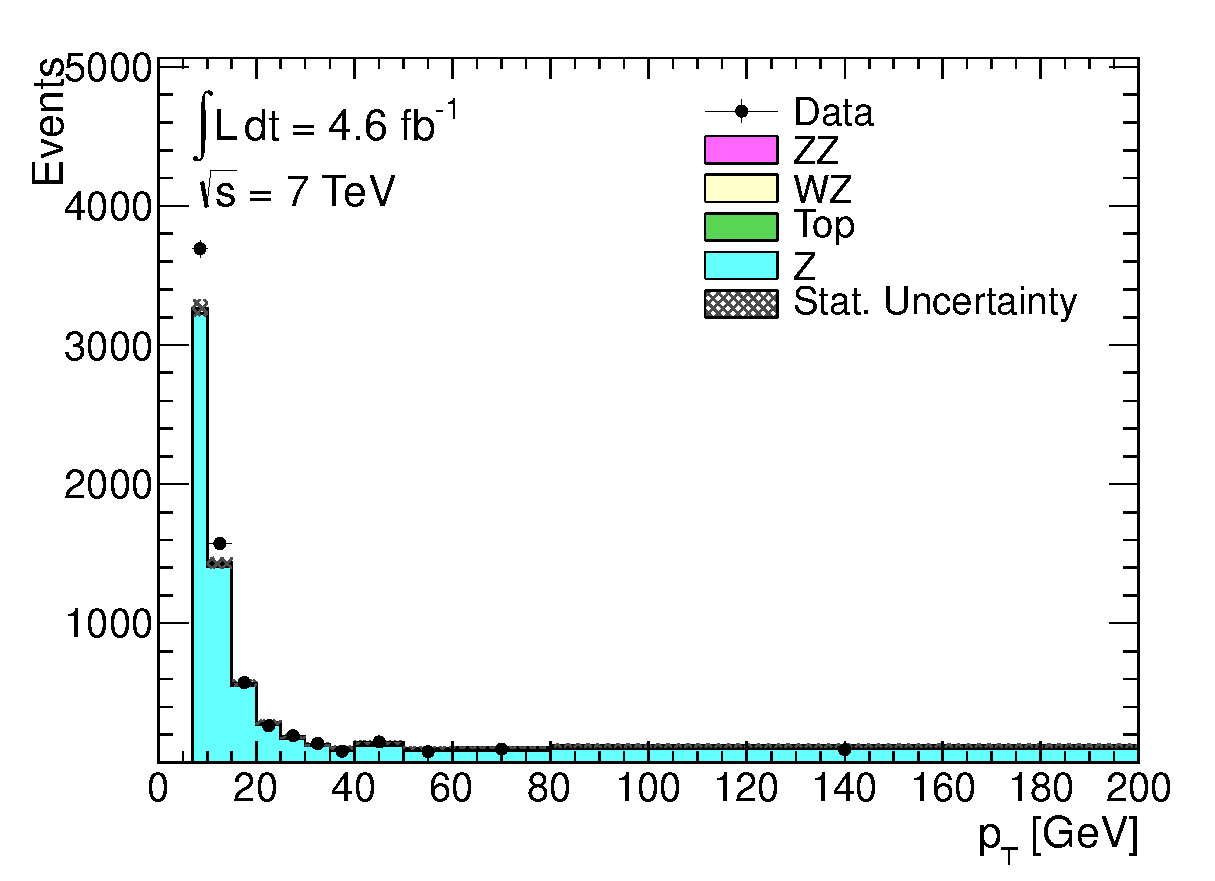
\includegraphics[width=0.47\textwidth]{ffDists7TeV/CentralEl_pt_L_lin}
        }
	\subfigure[Central Electron-Like-Jets]{
            \includegraphics[width=0.47\textwidth]{ffDists7TeV/CentralEl_pt_J_lin}
        }
	\subfigure[Selected Forward Electrons]{
            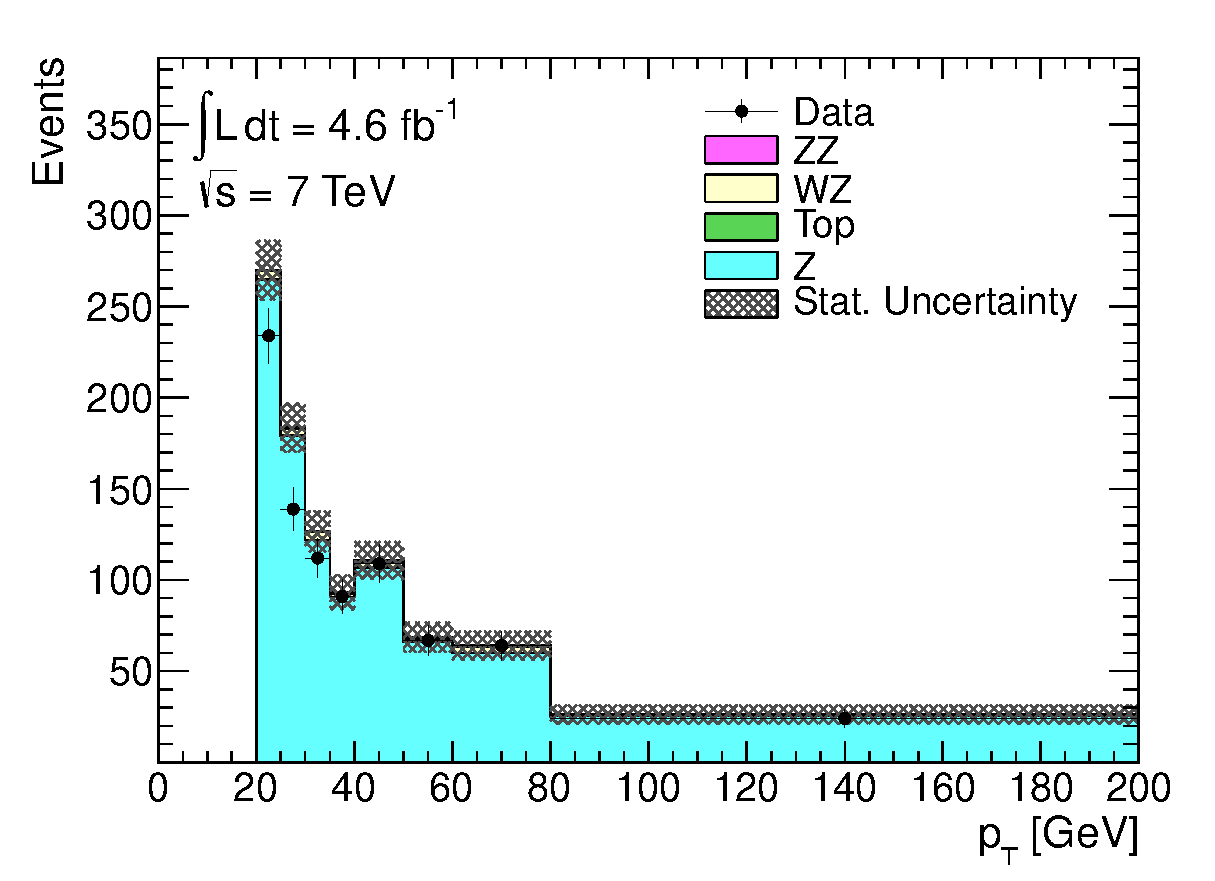
\includegraphics[width=0.47\textwidth]{ffDists7TeV/ForwardEl_pt_L_lin}
        }
	\subfigure[Forward Electron-Like-Jets]{
            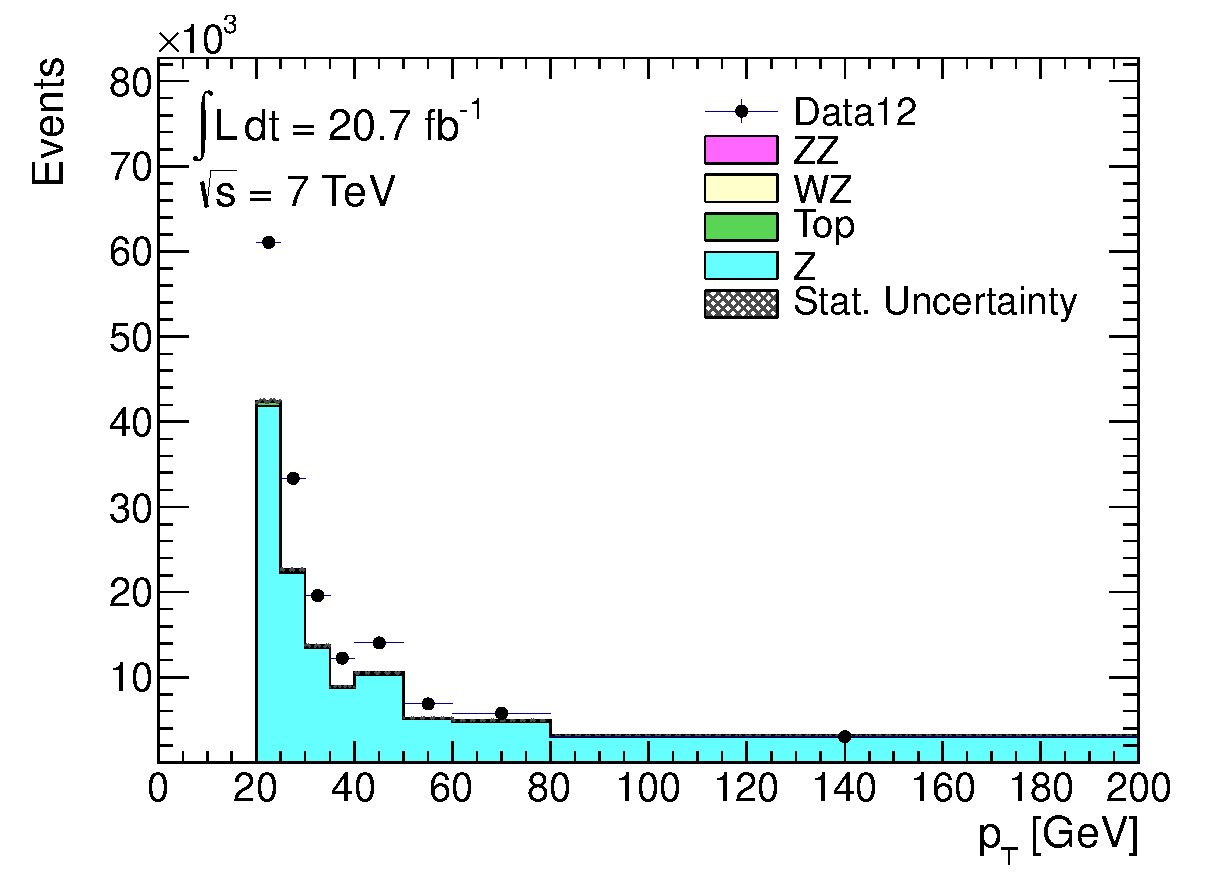
\includegraphics[width=0.47\textwidth]{ffDists7TeV/ForwardEl_pt_J_lin}
        }
	\subfigure[Selected Electrons]{
            \includegraphics[width=0.47\textwidth]{ffDists7TeV/AllEl_eta_L_lin}
        }
	\subfigure[Electron-Like-Jets]{
            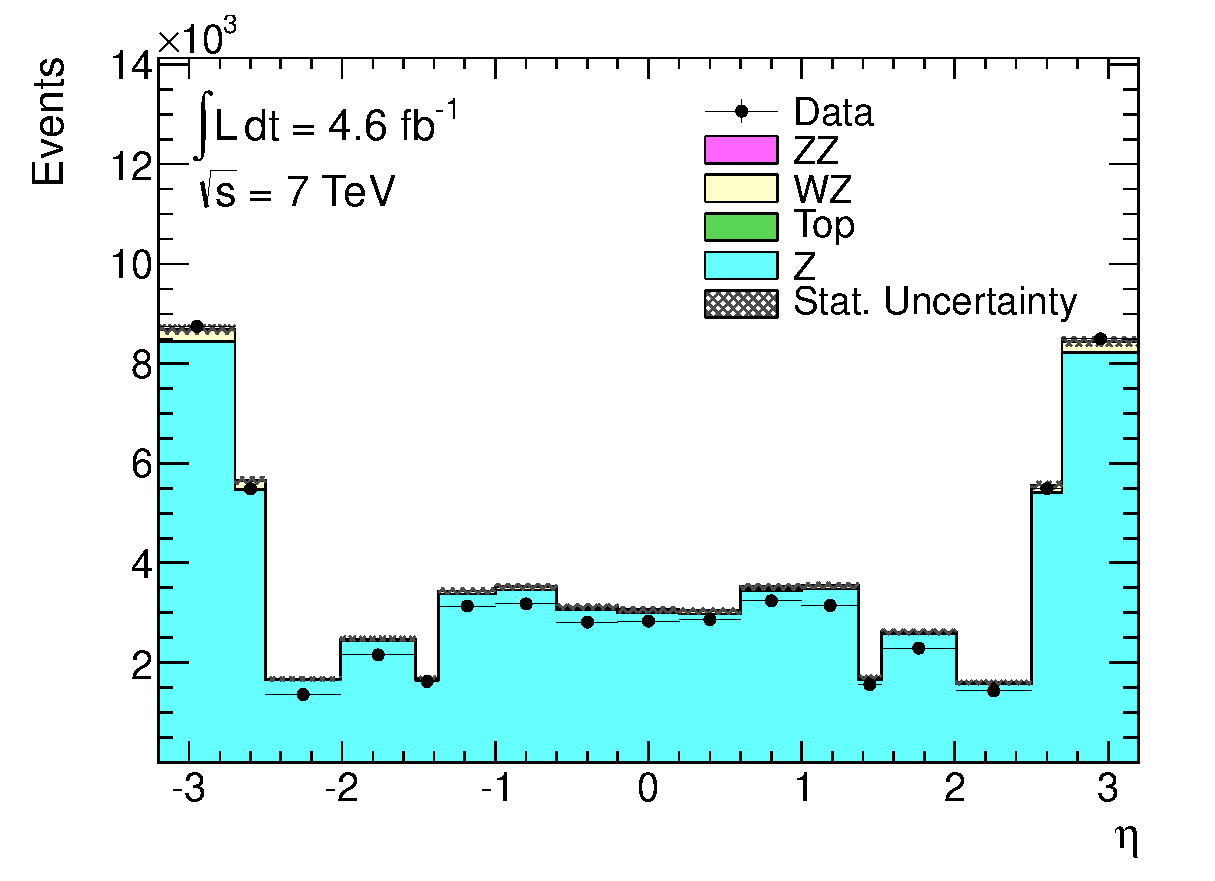
\includegraphics[width=0.47\textwidth]{ffDists7TeV/AllEl_eta_J_lin}
        }
    \caption[\pt\ and $\eta$ distributions for selected electrons $L$ and
    lepton-like-electrons $J$ in the \Z-tag sample for 7~\tev\ data.]
    {\pt\ and $\eta$ distributions for selected electrons $L$ and
    lepton-like-electrons $J$ in the \Z-tag sample for 7~\tev\ data. 
    For the \pt\ distributions, central and forward electrons are shown
    separately; for the $\eta$ distributions central and forward electrons are
    shown in the same plot.}
\label{fig:ljdist-el-seven} 
\end{figure}

\begin{figure}[h!]
\centering
	\subfigure[Selected Central Electrons]{
            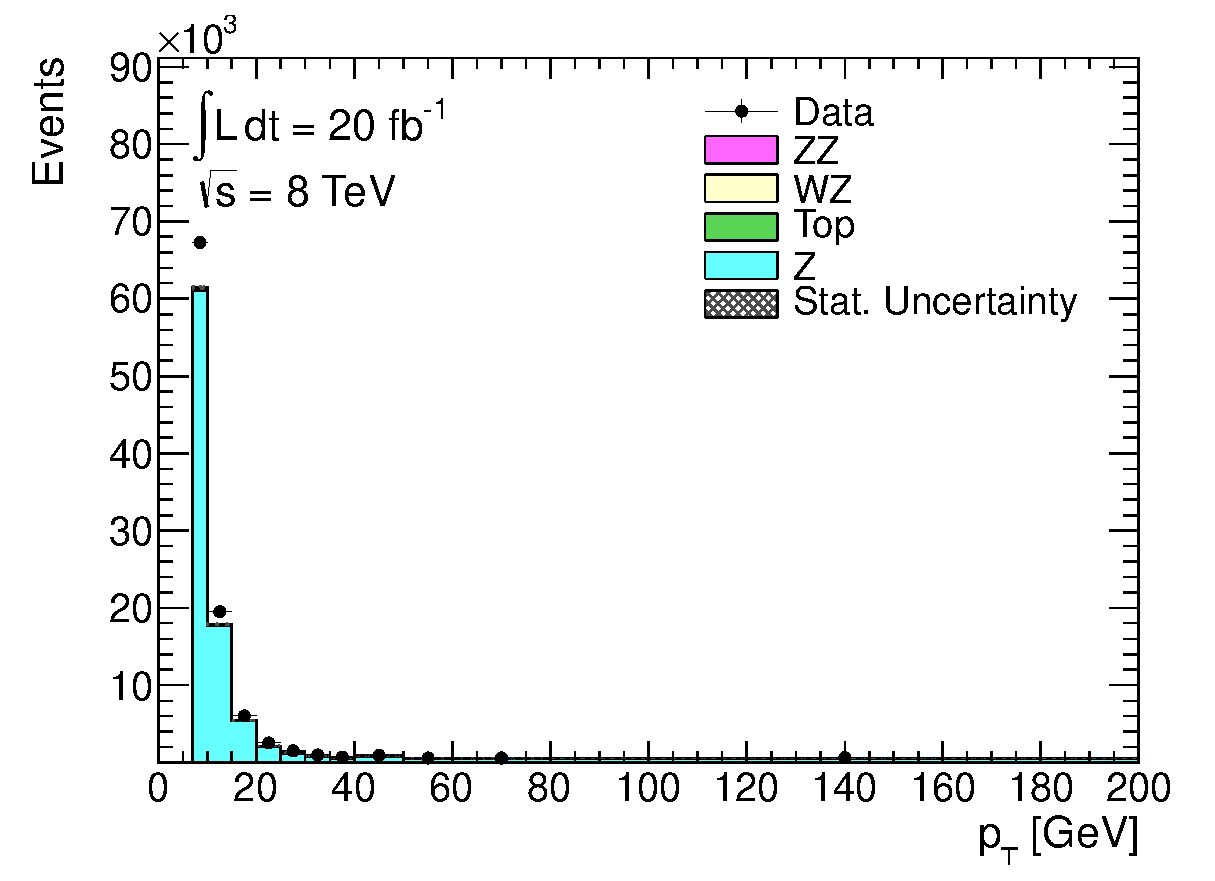
\includegraphics[width=0.47\textwidth]{ffDists8TeV/CentralEl_pt_L_lin}
        }
	\subfigure[Central Electron-Like-Jets]{
            \includegraphics[width=0.47\textwidth]{ffDists8TeV/CentralEl_pt_J_lin}
        }
	\subfigure[Selected Central Electrons]{
            \includegraphics[width=0.47\textwidth]{ffDists8TeV/AllEl_eta_L_lin}
        }
	\subfigure[Central Electron-Like-Jets]{
            \includegraphics[width=0.47\textwidth]{ffDists8TeV/AllEl_eta_J_lin}
        }
    \caption[\pt\ and $\eta$ distributions for selected electrons $L$ and
    electron-like-jets $J$ in the \Z-tag sample for 8~\tev\ data.]
    {\pt\ and $\eta$ distributions for selected electrons $L$ and
    lepton-like-electrons $J$ in the \Z-tag sample for 8~\tev\ data. 
   }
\label{fig:ljdist-el-eight} 
\end{figure}

\begin{figure}[h!]
\centering
\vspace{-8mm}
	\subfigure[Selected Central Muons]{
            \includegraphics[width=0.47\textwidth]{ffDists7TeV/CentralMu_pt_L_lin}
        }
	\subfigure[Central Muon-Like-Jets]{
            \includegraphics[width=0.47\textwidth]{ffDists7TeV/CentralMu_pt_J_lin}
        }
	\subfigure[Selected Forward Muons]{
            \includegraphics[width=0.47\textwidth]{ffDists7TeV/ForwardMu_pt_L_lin}
        }
	\subfigure[Forward Muon-Like-Jets]{
            \includegraphics[width=0.47\textwidth]{ffDists7TeV/ForwardMu_pt_J_lin}
        }
	\subfigure[Selected Calorimeter-Tagged Muons]{
            \includegraphics[width=0.47\textwidth]{ffDists7TeV/CaloMu_pt_J_lin}
        }
	\subfigure[Calorimeter-Tagged Muon-Like-Jets]{
            \includegraphics[width=0.47\textwidth]{ffDists7TeV/CaloMu_pt_J_lin}
        }
	\subfigure[Selected Muons]{
            \includegraphics[width=0.47\textwidth]{ffDists7TeV/AllMu_eta_L_lin}
        }
	\subfigure[Muon-Like-Jets]{
            \includegraphics[width=0.47\textwidth]{ffDists7TeV/AllMu_eta_J_lin}
        }
    \caption[\pt\ and $\eta$ distributions for selected muons $L$ and
    muons-like-jets $J$ in the \Z-tag sample for 7~\tev\ data.]
    {\small \pt\ and $\eta$ distributions for selected muons $L$ and
    lepton-like-muons $J$ in the \Z-tag sample for 7~\tev\ data. 
    For the \pt\ distributions, central, forward and calorimeter-tagged muons are shown
    separately; for the $\eta$ distributions all muons are
    shown in the same plot.}
\label{fig:ljdist-mu-seven} 
\end{figure}

\begin{figure}[h!]
\centering
\vspace{-8mm}
	\subfigure[Selected Central Muons]{
            \includegraphics[width=0.47\textwidth]{ffDists8TeV/CentralMu_pt_L_lin}
        }
	\subfigure[Central Muon-Like-Jets]{
            \includegraphics[width=0.47\textwidth]{ffDists8TeV/CentralMu_pt_J_lin}
        }
	\subfigure[Selected Forward Muons]{
            \includegraphics[width=0.47\textwidth]{ffDists8TeV/ForwardMu_pt_L_lin}
        }
	\subfigure[Forward Muon-Like-Jets]{
            \includegraphics[width=0.47\textwidth]{ffDists8TeV/ForwardMu_pt_J_lin}
        }
	\subfigure[Selected Calorimeter-Tagged Muons]{
            \includegraphics[width=0.47\textwidth]{ffDists8TeV/CaloMu_pt_J_lin}
        }
	\subfigure[Calorimeter-Tagged Muon-Like-Jets]{
            \includegraphics[width=0.47\textwidth]{ffDists8TeV/CaloMu_pt_J_lin}
        }
	\subfigure[Selected Muons]{
            \includegraphics[width=0.47\textwidth]{ffDists8TeV/AllMu_eta_L_lin}
        }
	\subfigure[Muon-Like-Jets]{
            \includegraphics[width=0.47\textwidth]{ffDists8TeV/AllMu_eta_J_lin}
        }
    \caption[\pt\ and $\eta$ distributions for selected muons $L$ and
    muon-like-jets $J$ in the \Z-tag sample for 8~\tev\ data.]
    {\small \pt\ and $\eta$ distributions for selected muons $L$ and
    lepton-like-muons $J$ in the \Z-tag sample for 8~\tev\ data. 
    For the \pt\ distributions, central, forward and calorimeter-tagged muons are shown
    separately; for the $\eta$ distributions all muons are
    shown in the same plot.}
\label{fig:ljdist-mu-eight} 
\end{figure}


The resulting \fakefactor s for electrons are shown in~\fig{ff-el-seven} for the
7~\tev\ analysis and in~\fig{ff-el-eight} for the 8~\tev\ analysis; the \fakefactor s
for muons are shown in~\fig{ff-mu-seven} for the
7~\tev\ analysis and in~\fig{ff-mu-eight} for the 8~\tev\ analysis. The
\ffactor\ estimated from \mcsim\ (blue triangles) is in reasonable agreement with
the \ffactor\ measured in data (black points). For the calculation of the
background, no use is made of the \ffactor\ estimated from \mcsim. The unparameterised \FF
s, used as the numerator in~\eqn{factorised-ff}, are given in~\tab{average-ff}.

\begin{table}[h!]
  \centering
  \small
  \begin{tabular}{lcc} 
    \hline\hline
    Lepton & $<\FF>$ 7~\tev &  $<\FF>$ 8~\tev \\
    \hline
    Central Electron            & \measStat{0.215}{\errSym{0.003}} & \measStat{0.133}{\errSym{0.001}}\\
    Forward Electron            & \measStat{0.030}{\errSym{0.001}} & - \\
    Central Muon                & \measStat{0.250}{\errSym{0.010}} & \measStat{0.395}{\errSym{0.005}}\\
    Forward Muon                & \measStat{0.782}{\errSym{0.199}} & \measStat{1.212}{\errSym{0.128}}\\
    Calorimeter-Tagged Muon     & \measStat{0.123}{\errSym{0.024}} & \measStat{0.098}{\errSym{0.007}} \\
    \hline\hline
  \end{tabular}
  \caption{Unparameterised (average) \ffactor s for different lepton types.}
  \label{table:average-ff}
\end{table}

\begin{figure}[h!]
\centering
	\subfigure[Central Electrons]{
            \includegraphics[width=0.47\textwidth]{FakeFactors7TeV/FF_CentralEl_pt_J_lin}
        }
	\subfigure[Forward Electrons]{
            \includegraphics[width=0.47\textwidth]{FakeFactors7TeV/FF_ForwardEl_pt_J_lin}
        }
	\subfigure[All Electrons]{
            \includegraphics[width=0.47\textwidth]{FakeFactors7TeV/FF_AllEl_eta_J_lin}
        }
    \caption[Electron \FakeFactor s as a function of \pt\ and $\eta$ for 7~\tev\ data.]
    {Electron \FakeFactor s as a function of \pt\ and $\eta$ for 7~\tev\ data. 
    For the distributions as a function of \pt\, central and forward electrons are shown
    separately; for the $\eta$ distributions the \ffactor\ for central and forward electrons are
    shown in the same plot. The black points show the \ffactor\ measured in
    data; the blue triangles show the value estimated by \mcsim.}
\label{fig:ff-el-seven} 
\end{figure}

\begin{figure}[h!]
\centering
	\subfigure[Central Electrons]{
            \includegraphics[width=0.47\textwidth]{FakeFactors8TeV/FF_CentralEl_pt_J_lin}
        }
	%\subfigure[Forward Electrons]{
            %\includegraphics[width=0.47\textwidth]{FakeFactors8TeV/FF_ForwardEl_pt_J_lin}
        %}
	\subfigure[Central Electrons]{
            \includegraphics[width=0.47\textwidth]{FakeFactors8TeV/FF_AllEl_eta_J_lin}
        }
    \caption[Electron \FakeFactor s as a function of \pt\ and $\eta$ for 8~\tev\ data.]
    {Electron \FakeFactor s as a function of \pt\ and $\eta$ for 8~\tev\ data. 
    The black points show the \ffactor\ measured in
    data; the blue triangles show the value estimated by \mcsim.}
\label{fig:ff-el-eight} 
\end{figure}

\begin{figure}[h!]
\centering
\vspace{-8mm}
	\subfigure[Central Muons]{
            \includegraphics[width=0.47\textwidth]{FakeFactors7TeV/FF_CentralMu_pt_J_lin}
        }
	\subfigure[Forward Muons]{
            \includegraphics[width=0.47\textwidth]{FakeFactors7TeV/FF_ForwardMu_pt_J_lin}
        }
	\subfigure[Calorimeter-Tagged Muons]{
            \includegraphics[width=0.47\textwidth]{FakeFactors7TeV/FF_CaloMu_pt_J_lin}
        }
	\subfigure[All Muons]{
            \includegraphics[width=0.47\textwidth]{FakeFactors7TeV/FF_AllMu_eta_J_lin}
        }
    \caption[Muon \FakeFactor s as a function of \pt\ and $\eta$ for 7~\tev\ data.]
    {Muon \FakeFactor s as a function of \pt\ and $\eta$ for 7~\tev\ data. 
    For the distributions as a function of \pt\, central, forward and calorimeter-tagged muons are shown
    separately; for the $\eta$ distributions the \ffactor\ all muons are
    shown in the same plot.The black points show the \ffactor\ measured in
    data; the blue triangles show the value estimated by \mc.}
\label{fig:ff-mu-seven} 
\end{figure}

\begin{figure}[h!]
\centering
\vspace{-8mm}
	\subfigure[Central Muons]{
            \includegraphics[width=0.47\textwidth]{FakeFactors8TeV/FF_CentralMu_pt_J_lin}
        }
	\subfigure[Forward Muons]{
            \includegraphics[width=0.47\textwidth]{FakeFactors8TeV/FF_ForwardMu_pt_J_lin}
        }
	\subfigure[Calorimeter-Tagged Muons]{
            \includegraphics[width=0.47\textwidth]{FakeFactors8TeV/FF_CaloMu_pt_J_lin}
        }
	\subfigure[All Muons]{
            \includegraphics[width=0.47\textwidth]{FakeFactors8TeV/FF_AllMu_eta_J_lin}
        }
    \caption[Muon \FakeFactor s as a function of \pt\ and $\eta$ for 8~\tev\ data.]
    {Muon \FakeFactor s as a function of \pt\ and $\eta$ for 8~\tev\ data. 
    For the distributions as a function of \pt\, central, forward and calorimeter-tagged muons are shown
    separately; for the $\eta$ distributions the \ffactor\ all muons are
    shown in the same plot.The black points show the \ffactor\ measured in
    data; the blue triangles show the value estimated by \mc.}
\label{fig:ff-mu-eight} 
\end{figure}

%\begin{figure}[h]
%\centering
%	\subfigure[Central Electrons]{
%            \includegraphics[width=0.47\textwidth]{FakeFactors/FF_CentralEl_pt_B_lin}
%        }
%	\subfigure[Forward Electrons]{
%            \includegraphics[width=0.47\textwidth]{FakeFactors/FF_ForwardEl_pt_B_lin}
%        }
%	\subfigure[All Electrons]{
%            \includegraphics[width=0.47\textwidth]{FakeFactors/FF_AllEl_eta_B_lin}
%        }
%    \caption[Electron \FakeFactor s as a function of \pt\ and $\eta$ for 7~\tev\ data.]
%    {Electron \FakeFactor s as a function of \pt\ and $\eta$ for 7~\tev\ data. 
%    For the distributions as a function of \pt\, central and forward electrons are shown
%    separately; for the $\eta$ distributions the \ffactor\ for central and forward electrons are
%    shown in the same plot. The black points show the \ffactor\ measured in
%    data; the blue triangles show the value estimated by \mc.}
%\label{fig:ff-el-seven} 
%\end{figure}

%\begin{figure}[h]
%\centering
%\vspace{-8mm}
%	\subfigure[Central Muons]{
%            \includegraphics[width=0.47\textwidth]{FakeFactors/FF_CentralMu_pt_B_lin}
%        }
%	\subfigure[Forward Muons]{
%            \includegraphics[width=0.47\textwidth]{FakeFactors/FF_ForwardMu_pt_B_lin}
%        }
%	\subfigure[Calorimeter-Tagged Muons]{
%            \includegraphics[width=0.47\textwidth]{FakeFactors/FF_CaloMu_pt_B_lin}
%        }
%	\subfigure[All Muons]{
%            \includegraphics[width=0.47\textwidth]{FakeFactors/FF_AllMu_eta_B_lin}
%        }
%    \caption[Muon \FakeFactor s as a function of \pt\ and $\eta$ for 7~\tev\ data.]
%    {Muon \FakeFactor s as a function of \pt\ and $\eta$ for 7~\tev\ data. 
%    For the distributions as a function of \pt\, central, forward and calorimeter-tagged muons are shown
%    separately; for the $\eta$ distributions the \ffactor\ all electrons are
%    shown in the same plot.The black points show the \ffactor\ measured in
%    data; the blue triangles show the value estimated by \mc.}
%\label{fig:ff-mu-seven} 
%\end{figure}

\subsection{Statistical and Systematic Uncertainties}

The statistical error from the \ffactor\ measurement is propagated to the
background estimate by repeating the calculation with the \ffactor\ shifted up and down
by their one-sigma statistical uncertainties. The variation of the predicted
background is then added in quadrature with the statistical uncertainty due to
limited numbers of observed $LLLJ$ and $LLJJ$ events. 
%In cases where no $LLLJ$
%or $LLJJ$ events are observed, the central value is taken as zero, and the
%uncertainty is set to correspond to a 68\% confidence level upper limit on the
%number of observed events of 1.29. This is scaled by the mean \ffactor\ for that
%channel.

Systematic uncertainties are estimated by varying the criteria used to define
the \lljet s as follows:
\begin{itemize}
\item Increasing the inverted isolation requirement to $>$20\%, $>$30\%, and
$>$40\%. For the 7~\tev\ data, where both track and calroimeter isolation are
used, the requirements on the two isolations are varied
simultaneously.
\item Increasing the inverted \dzero-significance requirement to
$>3.5$ (8~\tev\ only), $>4.0,>4.5,>5.0$.
%\item Requiring that the $J$ fail {\it either} the isolation {\it or} the
%identification (\dzero-significance) requirements, but not both.
\end{itemize}
The variations are designed to vary the composition of the different regions in
terms of the different sources of background leptons. Stability under these
variations indicates that the method is not highly sensitive to the composition
of the control region relative to the composition of the signal region. The
final background estimate is taken as the mean of the nominal background
estimate and the estimate obtained under each of these variations. The
statistical uncertainty is taken as the mean of the statistical uncertainties
from each variation and the systematic is taken as the RMS spread of the
estimates obtained from different variations.

\subsection{\mc\ Closure Test}

To demonstrate the validity of the background estimate method, a \mc\ closure
test is performed. The entire background estimate methodology described above is
applied to a \mc\ sample modelling the \ZX, \ttbar,
\singletop, \WZ\ and \WW\ backgrounds, to give a `background estimate' according
to the \mc. The \ffactor s are derived from the \mc, and are then applied
to $LLJJ$ and $LLLJ$ events from the \mc\ samples. The resulting `background
estimate' should then be in agreement with the number of $LLLL$ events passing the full
selection in the background \mc\ sample.

The results of the closure test are shown in~\tab{bg-est-mc-closure}. The
statistical uncertainties on the 8~\tev\ estimates are much larger, owing to the
size of the available \mc\ samples at 8~\tev\ being far smaller. In all cases, the
background estimate from \mc\ obtained using the \ffactor\ method is in good
agreement with the number of $LLLL$ events in the \mc.

\begin{table}
\small
\begin{tabular}{lcccc}
\hline\hline
    & \eeee & \mmmm & \eemm & \llll \\
\hline
\underline{\bf 7~\tev, \ZZ\ Selection} \\
$N_{BG}$ (\FFactor\ method) &  0.83 $\pm$ 0.29 &  0.04 $\pm$ 0.02 &  0.94 $\pm$ 0.36 &  1.81 $\pm$ 0.46 \\
$N_{LLLL}$ &  0.69 $\pm$ 0.25 &  0.01 $\pm$ 0.01 &  0.79 $\pm$ 0.28 &  1.49 $\pm$ 0.37 \\
\hline
\underline{\bf 7~\tev, \ZZs\ Selection} \\
$N_{BG}$ &  4.22 $\pm$ 0.81 &  -0.01 $\pm$ 0.07  &  4.54 $\pm$ 0.83 &  8.75 $\pm$ 1.17 \\
$N_{LLLL}$ &  3.80 $\pm$ 0.92 &  0.06 $\pm$ 0.05 &  4.41 $\pm$ 0.92 &  8.26 $\pm$ 1.30 \\
\hline
\underline{\bf 8~\tev, \ZZ\ Selection} \\
$N_{BG}$ &  2.40 $\pm$ 2.01 &  0.19 $\pm$ 0.05 &  2.16 $\pm$ 1.95  &  4.74 $\pm$ 2.80 \\
$N_{LLLL}$ &  2.99 $\pm$ 2.58 &  0.04 $\pm$ 0.04 &  0.62 $\pm$ 0.17 &  3.66 $\pm$ 2.58 \\
\hline\hline
\end{tabular}
\caption{Results of the \mc\ closure test for the data driven background
estimate. }
\label{table:bg-est-mc-closure}
\end{table}

\subsection{Results}

The number of observed $LLLJ$ and $LLJJ$ events, these quantities multiplied by
the \fakefactor\ (squared in the latter case), the estimated correction due to
contamination from \ZZ\ events, and the resulting background estimate for the `nominal' $J$ definition are shown
in~\tab{bg-est-nominal-seven} for the 7~\tev\
data and in~\tab{bg-est-nominal-eight} for the 8~\tev\ data. The \ffactor\ is
applied individually to each $J$, parameterised by the \pt\ and $\eta$ of the
$J$. The background
estimates under each of the systematic variations described in the previous section are
shown in~\tabs{bg-est-syst-seven}{bg-est-syst-eight}. The results are observed
to be rather stable under the systematic variations, within the large statistica
uncertainties.

In the \mmmm\ channel the number of observed $LLLJ$ and $LLJJ$ events is small,
and so the final background estimate is zero due to \NLLJJ\ being larger than
\NLLLJ. In this case, the final result is quoted as a truncated Gaussian, with
mean at zero and sigma equal to the estimated uncertainty. This procedure gives a
conservative upper limit for the background in that channel.
The final data-driven background estimates are shown
in~\tab{bg-est-final-dd}.

\begin{table}[htbp]
\footnotesize
\renewcommand\arraystretch{1.2}
\centering
\begin{tabular}{lcccc}
\hline\hline
 7~\tev, \ZZ\ & \eeee\ & \mmmm\ & \eemm\ & \llll\ \\
 \hline
$N_{LLLJ}$                          &  23.00 $\pm$ 4.80 &  1.00 $\pm$ 1.00 &  22.00 $\pm$ 4.69 &  46.00 $\pm$ 6.78 \\
($+$) $N_{LLLJ} \times FF$          &  1.75 $\pm$ 0.49 &  0.19 $\pm$ 0.19 &  2.17 $\pm$ 0.76 &  4.11 $\pm$ 0.92 \\
%$N_{LLLJ} \times FF$ Up            &  1.94 $\pm$ 0.54 &  0.21 $\pm$ 0.21 &  2.65 $\pm$ 1.00 &  4.80 $\pm$ 1.16 \\
%$N_{LLLJ} \times FF$ Down          &  1.56 $\pm$ 0.45 &  0.16 $\pm$ 0.16 &  1.69 $\pm$ 0.56 &  3.41 $\pm$ 0.74 \\
($-$) $N_{LLLJ}^{ZZ,MC}  \times FF$ &  0.35 $\pm$ 0.01 &  0.35 $\pm$ 0.02 &  0.72 $\pm$ 0.02 &  1.42 $\pm$ 0.04 \\
$N_{LLJJ}$                          &  101.00 $\pm$ 10.05 &  4.00 $\pm$ 2.00 &  87.00 $\pm$ 9.33 &  192.00 $\pm$ 13.86 \\
($-$) $N_{LLJJ} \times FF^{2}$      &  1.07 $\pm$ 0.19 &  0.42 $\pm$ 0.23 &  0.94 $\pm$ 0.20 &  2.43 $\pm$ 0.36 \\
% $N_{LLJJ} \times FF$ Up           &  1.29 $\pm$ 0.22 &  0.71 $\pm$ 0.39 &  1.20 $\pm$ 0.27 &  3.19 $\pm$ 0.52 \\
%$N_{LLJJ} \times FF$ Down          &  0.88 $\pm$ 0.16 &  0.20 $\pm$ 0.11 &  0.71 $\pm$ 0.15 &  1.79 $\pm$ 0.24 \\
($+$) $N_{LLJJ}^{ZZ,MC}\times FF^2$ &  0.00 $\pm$ 0.00 &  0.00 $\pm$ 0.00 &  0.01 $\pm$ 0.00 &  0.01 $\pm$ 0.00 \\
\hline
$N_{BG}$                            &  0.33 $\pm$ 0.53 $^{+0.33}_{-0.04}$ &  -0.58 $\pm$ 0.30 $^{+0.38}_{-0.08}$ &  0.52 $\pm$ 0.78 $^{+0.93}_{-0.04}$ &  0.27 $\pm$ 0.99 $^{+1.34}_{-0.38}$ \\
\hline\hline
\\
\hline\hline
 7~\tev, \ZZs\ & \eeee\ & \mmmm\ & \eemm\ & \llll\ \\
\hline
$N_{LLLJ}$                          &                     75.00 $\pm$ 8.66 &                      4.00 $\pm$ 2.00 &                    95.00 $\pm$ 9.75 &                   174.00 $\pm$ 13.19 \\
($+$) $N_{LLLJ} \times FF$          &                      9.87 $\pm$ 1.42 &                      0.86 $\pm$ 0.44 &                    16.31 $\pm$ 2.72 &                     27.04 $\pm$ 3.10 \\
%$N_{LLLJ} \times FF$ Up            &                     10.64 $\pm$ 1.51 &                      1.10 $\pm$ 0.57 &                    20.05 $\pm$ 4.59 &                     31.78 $\pm$ 4.87 \\
%$N_{LLLJ} \times FF$ Down          &                      9.11 $\pm$ 1.32 &                      0.63 $\pm$ 0.32 &                    12.80 $\pm$ 1.72 &                     22.53 $\pm$ 2.19 \\
($-$) $N_{LLLJ}^{ZZ,MC}  \times FF$ &                      0.63 $\pm$ 0.01 &                      0.64 $\pm$ 0.03 &                     1.16 $\pm$ 0.03 &                      2.43 $\pm$ 0.04 \\
$N_{LLJJ}$                          &                   297.00 $\pm$ 17.23 &                     15.00 $\pm$ 3.87 &                  240.00 $\pm$ 15.49 &                   552.00 $\pm$ 23.49 \\
($-$) $N_{LLJJ} \times FF^{2}$      &                      5.84 $\pm$ 0.53 &                      1.43 $\pm$ 0.46 &                     5.71 $\pm$ 0.58 &                     12.98 $\pm$ 0.91 \\
% $N_{LLJJ} \times FF$ Up           &                      6.75 $\pm$ 0.61 &                      2.54 $\pm$ 0.85 &                     7.17 $\pm$ 0.74 &                     16.46 $\pm$ 1.28 \\
%$N_{LLJJ} \times FF$ Down          &                      5.00 $\pm$ 0.47 &                      0.60 $\pm$ 0.19 &                     4.44 $\pm$ 0.46 &                     10.03 $\pm$ 0.68 \\
($+$) $N_{LLJJ}^{ZZ,MC}\times FF^2$ &                      0.01 $\pm$ 0.00 &                      0.01 $\pm$ 0.00 &                     0.02 $\pm$ 0.00 &                      0.04 $\pm$ 0.00 \\
\hline                                  
$N_{BG}$                            &  3.42 $\pm$ 1.52 $^{+0.47}_{-0.13}$ &  -1.21 $\pm$ 0.64 $^{+0.89}_{-0.24}$ &  9.47 $\pm$ 2.78 $^{+3.42}_{-1.96}$ &  11.67 $\pm$ 3.23 $^{+3.65}_{-0.94}$ \\
\hline\hline
\end{tabular}
\renewcommand\arraystretch{1.}
\caption[Details of the background estimate for 4.6~\ifb\ of 7~\tev\
data.]{\small Details of the background estimate for 4.6~\ifb\ of 7~\tev\
data. The top table shows the background estimate for the \ZZ\ selection and the
bottom for the \ZZs\ selection. In each table, first row
shows the number of observed \LLLJ\ events. The second row shows this quantity
scaled by the \ffactor\ (applied on an event by event basis), and the third row
the MC estimated number of \ZZ\ events identified as \LLJJ, scaled by the
\fakefactor. The fourth and
fifth rows
show the number of observed \LLJJ\ events, and the number of \LLJJ\ events
scaled by the \ffactor, and the sixth row the estimated number of \ZZ\ events
identified as \LLLJ, scaled by the \ffactor. The resulting background estimate
is shown in the last row, and is the sum of the rows indicated with `$(+)$',
minus the sum of the rows indicated with `$(-)$'. The first error is due to
statistical uncertainty on the number of observed \LLLJ\ and \LLJJ\ events,
while the
second error is due to statistical uncertainty on the \ffactor.}
\label{table:bg-est-nominal-seven}
\end{table}

\begin{table}[htbp]
\footnotesize
\renewcommand\arraystretch{1.2}
\centering
\begin{tabular}{lcccc}
\hline\hline
 8~\tev, \ZZ & \eeee\ & \mmmm\ & \eemm\ & \llll\ \\
\hline
$N_{LLLJ}$                          &  166.00 $\pm$ 12.88 &  9.00 $\pm$ 3.00 &  114.00 $\pm$ 10.68 &  289.00 $\pm$ 17.00 \\
($+$) $N_{LLLJ} \times FF$          &  17.71 $\pm$ 1.60 &  5.60 $\pm$ 2.30 &  17.52 $\pm$ 2.95 &  40.83 $\pm$ 4.07 \\
%$N_{LLLJ} \times FF$ Up            &  18.12 $\pm$ 1.62 &  6.90 $\pm$ 2.99 &  19.94 $\pm$ 3.82 &  44.96 $\pm$ 5.12 \\
%$N_{LLLJ} \times FF$ Down          &  17.30 $\pm$ 1.57 &  4.30 $\pm$ 1.64 &  15.09 $\pm$ 2.14 &  36.70 $\pm$ 3.12 \\
($-$) $N_{LLLJ}^{ZZ,MC}  \times FF$ &  0.80 $\pm$ 0.02 &  1.90 $\pm$ 0.07 &  3.09 $\pm$ 0.12 &  5.79 $\pm$ 0.15 \\
$N_{LLJJ}$ &  661.00 $\pm$ 25.71    &  11.00 $\pm$ 3.32 &  443.00 $\pm$ 21.05 &  1115.00 $\pm$ 33.39 \\
($-$) $N_{LLJJ} \times FF^{2}$      &  7.05 $\pm$ 0.36 &  1.58 $\pm$ 0.54 &  5.77 $\pm$ 0.53 &  14.39 $\pm$ 0.84 \\
% $N_{LLJJ} \times FF$ Up           &  7.38 $\pm$ 0.38 &  1.97 $\pm$ 0.68 &  6.43 $\pm$ 0.71 &  15.79 $\pm$ 1.05 \\
%$N_{LLJJ} \times FF$ Down          &  6.72 $\pm$ 0.35 &  1.22 $\pm$ 0.42 &  5.15 $\pm$ 0.40 &  13.09 $\pm$ 0.68 \\
($+$) $N_{LLJJ}^{ZZ,MC}\times FF^2$ &  0.01 $\pm$ 0.00 &  0.02 $\pm$ 0.01 &  0.02 $\pm$ 0.00 &  0.05 $\pm$ 0.01 \\
\hline
$N_{BG}$                            &  9.88 $\pm$ 1.64 $^{+0.86}_{-0.05}$ &  2.14 $\pm$ 2.37 $^{+2.79}_{-0.49}$ &  8.68 $\pm$ 3.00 $^{+4.83}_{-1.18}$ &  20.70 $\pm$ 4.16 $^{+8.48}_{-1.72}$ \\
%$N_{LLLL}$ &  62.00 $\pm$ 7.87 &  85.00 $\pm$ 9.22 &  158.00 $\pm$ 12.57 &  305.00 $\pm$ 17.46 \\
%$N_{LLLL}^{ZZ MC}$ &  57.92 $\pm$ 0.44 &  84.30 $\pm$ 0.54 &  136.30 $\pm$ 0.94 &  278.52 $\pm$ 1.17 \\
\hline\hline
\end{tabular}
\renewcommand\arraystretch{1.}
\caption[Details of the background estimate for 20~\ifb\ of 8~\tev\ data. ]
{\small Details of the background estimate for 20~\ifb\ of 8~\tev\ data. The first row
shows the number of observed \LLLJ\ events. The second row shows this quantity
scaled by the \ffactor\ (applied on an event by event basis), and the third row
the MC estimated number of \ZZ\ events identified as \LLJJ, scaled by the
\fakefactor. The fourth and
fifth rows
show the number of observed \LLJJ\ events, and the number of \LLJJ\ events
scaled by the \ffactor, and the sixth row the estimated number of \ZZ\ events
identified as \LLLJ, scaled by the \ffactor. The resulting background estimate
is shown in the last row, and is the sum of the rows indicated with `$(+)$',
minus the sum of the rows indicated with `$(-)$'. The first error is due to
statistical uncertainty on the number of observed \LLLJ\ and \LLJJ\ events,
while the
second error is due to statistical uncertainty on the \ffactor.}
\label{table:bg-est-nominal-eight}
\end{table}

%%%%%%%%%%%%%%%%%%%%%%%%%%
% Systematic variations

% Systematic variations, 7 TeV
\begin{table}
\centering
\footnotesize
\renewcommand\arraystretch{1.2}
\begin{tabular}{lcccc}
\hline\hline
 7~\tev, \ZZ & \eeee\ & \mmmm\ & \eemm\ & \llll \\
\hline
                      Nominal$J$  &  0.33 $\pm$ 0.53 $^{+0.33}_{-0.04}$ &  -0.63 $\pm$ 0.32 $^{+0.52}_{-0.50}$ &   0.51 $\pm$ 0.77 $^{+0.90}_{-0.02}$ &   0.20 $\pm$ 0.99 $^{+0.73}_{-0.54}$ \\
            $|\dzerosig| >$ 0.40  &  0.33 $\pm$ 0.53 $^{+0.33}_{-0.04}$ &  -0.68 $\pm$ 0.36 $^{+0.58}_{-0.68}$ &   0.63 $\pm$ 0.76 $^{+0.94}_{-0.09}$ &   0.27 $\pm$ 1.00 $^{+0.59}_{-0.53}$ \\
            $|\dzerosig| >$ 0.45  &  0.33 $\pm$ 0.53 $^{+0.33}_{-0.04}$ &  -0.67 $\pm$ 0.36 $^{+0.57}_{-0.68}$ &   0.65 $\pm$ 0.76 $^{+0.92}_{-0.10}$ &   0.31 $\pm$ 1.00 $^{+0.57}_{-0.51}$ \\
            $|\dzerosig| >$ 0.50  &  0.33 $\pm$ 0.53 $^{+0.33}_{-0.04}$ &  -0.41 $\pm$ 0.27 $^{+0.32}_{-0.11}$ &   0.66 $\pm$ 0.76 $^{+0.91}_{-0.11}$ &   0.58 $\pm$ 0.97 $^{+1.13}_{-0.25}$ \\
TrackIso$>${0.2}                  &  0.35 $\pm$ 0.54 $^{+0.32}_{-0.03}$ &  -0.69 $\pm$ 0.37 $^{+0.60}_{-0.74}$ &   0.48 $\pm$ 0.75 $^{+0.89}_{-0.04}$ &   0.14 $\pm$ 1.00 $^{+0.60}_{-0.47}$ \\
TrackIso$>${0.3}                  &  0.37 $\pm$ 0.55 $^{+0.32}_{-0.03}$ &  -0.72 $\pm$ 0.42 $^{+0.47}_{-0.42}$ &   0.62 $\pm$ 0.79 $^{+0.89}_{-0.09}$ &   0.27 $\pm$ 1.01 $^{+0.79}_{-0.41}$ \\
TrackIso$>${0.4}                  &  0.39 $\pm$ 0.57 $^{+0.31}_{-0.04}$ &  -0.99 $\pm$ 0.60 $^{+0.73}_{-0.97}$ &   0.75 $\pm$ 0.88 $^{+0.95}_{-0.13}$ &   0.16 $\pm$ 1.16 $^{+0.63}_{-0.29}$ \\
TrackIso$>${0.5}                  &  0.19 $\pm$ 0.56 $^{+0.29}_{-0.05}$ &  -0.82 $\pm$ 0.61 $^{+0.67}_{-1.01}$ &  -0.09 $\pm$ 0.60 $^{+0.57}_{-0.23}$ &  -0.72 $\pm$ 0.97 $^{+0.95}_{-0.15}$ \\
\hline\hline
\\
\hline\hline
 7~\tev, \ZZs & \eeee\ & \mmmm\ & \eemm\ & \llll \\
                      Nominal$J$  &  3.42 $\pm$ 1.52 $^{+0.47}_{-0.13}$ &  -1.27 $\pm$ 0.63 $^{+1.02}_{-0.79}$ &  8.10 $\pm$ 2.13 $^{+1.80}_{-0.55}$ &  10.25 $\pm$ 2.68 $^{+1.48}_{-0.60}$ \\
            $|\dzerosig| >$ 0.40  &  3.42 $\pm$ 1.52 $^{+0.47}_{-0.13}$ &  -1.03 $\pm$ 0.58 $^{+0.90}_{-0.75}$ &  8.32 $\pm$ 2.13 $^{+1.90}_{-0.67}$ &  10.70 $\pm$ 2.67 $^{+1.62}_{-0.36}$ \\
            $|\dzerosig| >$ 0.45  &  3.42 $\pm$ 1.52 $^{+0.47}_{-0.13}$ &  -1.24 $\pm$ 0.53 $^{+0.95}_{-0.83}$ &  8.39 $\pm$ 2.13 $^{+1.90}_{-0.70}$ &  10.57 $\pm$ 2.67 $^{+1.54}_{-0.38}$ \\
            $|\dzerosig| >$ 0.50  &  3.42 $\pm$ 1.52 $^{+0.47}_{-0.13}$ &  -0.92 $\pm$ 0.47 $^{+0.67}_{-0.23}$ &  8.41 $\pm$ 2.13 $^{+1.88}_{-0.71}$ &  10.90 $\pm$ 2.66 $^{+2.12}_{-0.10}$ \\
TrackIso$>${0.2}                  &  3.17 $\pm$ 1.52 $^{+0.43}_{-0.16}$ &  -1.32 $\pm$ 0.68 $^{+1.11}_{-1.10}$ &  7.82 $\pm$ 2.16 $^{+1.86}_{-0.64}$ &   9.67 $\pm$ 2.73 $^{+1.19}_{-0.63}$ \\
TrackIso$>${0.3}                  &  3.28 $\pm$ 1.54 $^{+0.44}_{-0.15}$ &  -1.55 $\pm$ 0.66 $^{+1.01}_{-0.81}$ &  8.16 $\pm$ 2.26 $^{+1.90}_{-0.74}$ &   9.89 $\pm$ 2.82 $^{+1.53}_{-0.41}$ \\
TrackIso$>${0.4}                  &  3.78 $\pm$ 1.60 $^{+0.47}_{-0.10}$ &  -1.77 $\pm$ 0.85 $^{+1.25}_{-1.31}$ &  9.01 $\pm$ 2.58 $^{+2.37}_{-1.18}$ &  11.02 $\pm$ 3.15 $^{+1.54}_{-0.17}$ \\
TrackIso$>${0.5}                  &  3.69 $\pm$ 1.64 $^{+0.45}_{-0.11}$ &  -1.56 $\pm$ 0.96 $^{+1.19}_{-1.36}$ &  6.96 $\pm$ 2.23 $^{+1.09}_{-0.12}$ &   9.08 $\pm$ 2.93 $^{+1.42}_{-0.18}$ \\
\hline
\hline\hline                       
\end{tabular}           
\caption[Comparison of background estimates for the 7~\tev\ analysis, using different
criteria to define the \lljet s $J$.]{Comparison of background estimates for the
7~\tev\ analysis, using different
criteria to define the \lljet s $J$. The first column indicates the variation
made to $J$ from the nominal definition given in~\tab{J-def}. The top table shows estimates for the \ZZ\
selection, the bottom for the \ZZs.}
\label{table:bg-est-syst-seven}
\renewcommand\arraystretch{1.0}
\end{table}            

% Systematic variations, 8 TeV
\begin{table}
\centering
\footnotesize
\renewcommand\arraystretch{1.2}
\begin{tabular}{lcccc}
\hline\hline
 8~\tev, \ZZ & \eeee\ & \mmmm\ & \eemm\ & \llll\ \\
\hline
Nominal $J$          &   9.01 $\pm$ 1.56 $^{+0.85}_{-0.05}$ &    1.98 $\pm$ 2.32 $^{+2.82}_{-0.49}$ &      8.35 $\pm$ 2.99 $^{+4.84}_{-1.18}$ &     19.34 $\pm$ 4.10 $^{+8.51}_{-1.72}$ \\
$|\dzerosig| >$ 0.35 &   9.01 $\pm$ 1.56 $^{+0.85}_{-0.05}$ &    0.70 $\pm$ 1.81 $^{+1.93}_{-0.07}$ &      5.31 $\pm$ 2.17 $^{+3.11}_{-0.20}$ &     15.02 $\pm$ 3.23 $^{+5.89}_{-0.32}$ \\
$|\dzerosig| >$ 0.40 &   9.01 $\pm$ 1.56 $^{+0.85}_{-0.05}$ &    0.83 $\pm$ 1.84 $^{+1.83}_{-0.09}$ &      3.55 $\pm$ 1.55 $^{+2.06}_{-0.37}$ &     13.39 $\pm$ 2.87 $^{+4.74}_{-0.24}$ \\
$|\dzerosig| >$ 0.45 &   9.01 $\pm$ 1.56 $^{+0.85}_{-0.05}$ &    0.93 $\pm$ 1.88 $^{+1.77}_{-0.12}$ &      3.64 $\pm$ 1.56 $^{+1.98}_{-0.35}$ &     13.58 $\pm$ 2.90 $^{+4.60}_{-0.18}$ \\
$|\dzerosig| >$ 0.50 &   9.01 $\pm$ 1.56 $^{+0.85}_{-0.05}$ &    1.06 $\pm$ 1.98 $^{+1.78}_{-0.16}$ &      3.37 $\pm$ 1.53 $^{+1.88}_{-0.37}$ &     13.44 $\pm$ 2.96 $^{+4.52}_{-0.17}$ \\
\ptconetwentygt{0.2} &   9.29 $\pm$ 1.58 $^{+0.83}_{-0.06}$ &    2.36 $\pm$ 2.44 $^{+2.58}_{-0.58}$ &      8.20 $\pm$ 3.00 $^{+4.67}_{-1.23}$ &     19.85 $\pm$ 4.18 $^{+8.07}_{-1.87}$ \\
\ptconetwentygt{0.3} &   9.40 $\pm$ 1.61 $^{+0.80}_{-0.06}$ &    2.23 $\pm$ 2.59 $^{+2.24}_{-0.56}$ &      8.21 $\pm$ 3.04 $^{+4.45}_{-1.28}$ &     19.84 $\pm$ 4.31 $^{+7.49}_{-1.90}$ \\
\ptconetwentygt{0.4} &   9.69 $\pm$ 1.64 $^{+0.80}_{-0.07}$ &    2.74 $\pm$ 3.12 $^{+2.49}_{-0.76}$ &      9.12 $\pm$ 3.56 $^{+4.89}_{-1.64}$ &     21.55 $\pm$ 5.01 $^{+8.18}_{-2.47}$ \\
\ptconetwentygt{0.5} &   9.89 $\pm$ 1.64 $^{+0.80}_{-0.07}$ &    0.71 $\pm$ 2.53 $^{+1.93}_{-0.04}$ &     10.03 $\pm$ 4.09 $^{+5.51}_{-1.96}$ &     20.63 $\pm$ 5.08 $^{+8.25}_{-2.08}$ \\
\hline\hline            
\end{tabular}           
\caption[Comparison of background estimates for the 8~\tev\ analysis, using different
criteria to define the \lljet s $J$.]{Comparison of background estimates for the
8~\tev\ analysis, using different
criteria to define the \lljet s $J$. The first column indicates the variation
made to $J$ from the nominal definition given in~\tab{J-def}. }
\label{table:bg-est-syst-eight}
\renewcommand\arraystretch{1.0}
\end{table}            


\begin{table}
\footnotesize
\begin{tabular}{l|c|c|c|c}
\hline\hline
 & 4e & 4mu & 2e2mu & 4l \\
\hline
 \ZZ, 7~\tev\  &  0.33 $^{+0.63}_{-0.54}\;\pm0.06$  &  $<0.71$ &  0.53 $^{+1.16}_{-0.77}\;\pm0.25$ &   0.15 $^{+1.26}_{-1.08}\;\pm0.35$ \\
 \ZZs, 8~\tev\ &  3.45 $^{+1.61}_{-1.55}\;\pm0.19$  &  $<1.25$ &  8.15 $^{+2.88}_{-2.31}\;\pm0.55$ &  10.26 $^{+3.19}_{-2.81}\;\pm0.63$ \\
 \ZZ, 8~\tev\  &   9.26 $^{+1.79}_{-1.59}\;\pm0.32$ &  1.50 $^{+3.14}_{-2.30}\;\pm0.77$ &   6.64 $^{+4.54}_{-2.78}\;\pm2.51$ &    17.41 $^{+7.72}_{-4.04}\;\pm3.25$ \\
\hline\hline
\end{tabular}
\caption[Final data-driven fake background estimates.]
{Final data-driven fake background estimates. The first error is statistical, the second
is systematic.}
\end{table}
\label{table:bg-est-final-dd}

\subsection{Cross Check with Same-Sign Events}

An additional cross check of the background estimate is performed by estimating
the background using a data sample composed of events passing the full event
selection, but with one opposite-signed \dilep\ pair and one same-signed \dilep\
pair (termed OS-SS). The majority of the irreducible backgrounds due to \Zgamma,
\Z+light-jets, \ttbar, \WW\ and \WZ\ events will contribute to the OS-SS
selection at the same rate as to the signal selection with two oppositely-signed
pairs (SS-SS). The exception to this is \Zbb, where leptons from heavy flavour
decay will tend to be oppositely-charged in the two jets. There will be
significant contamination to this control region from \ZZ\ events where one
lepton has its charged misidentified. This is estimated from \mc, and subtracted
from the observed OS-SS events to give the background estimate by this method. 

The number of observed events passing the OS-SS selection, the
estimated \ZZ\ contamination and the resulting background estimate are shown
in~\tab{bg-est-ss} for the 8~\tev\ analysis (this cross-check was not performed
for the 7~\tev\ data). The results are in good agreement with the background
estimate from the \ffactor\ method.

\begin{table}
\centering
\footnotesize
  \begin{tabular}{lcccc}
    \hline\hline
    & \eeee & \mmmm & \eemm & \llll \\
    \hline
    Observed OS-SS Events & 8 & 0 & 16 & 24 \\
    Expected \ZZ\ OS-SS & 2.65 \errSym{0.10} & 0.03 \errSym{0.01} & 3.19 \errSym{0.16} & 5.95 \errSym{0.19} \\
    \hline
    Bkg. Estimate (OS-SS)  & 5.35 \errSym{2.83} & $<$ 1.27 & 12.81
    \errSym{4.00} & 18.05 \errSym{2.83} \\
    Bkg. Estimate (\ffactor) & \ZZEightTeVDDBgEstZZEEEE &
    \ZZEightTeVDDBgEstZZMMMM & \ZZEightTeVDDBgEstZZEEMM & \ZZEightTeVDDBgEstZZLLLL \\
    \hline\hline
  \end{tabular}
      \caption[Background estimate cross check to the 8~\tev\ \ZZ\ analysis using same-sign events.]
      {Background estimate cross check to the 8~\tev\ \ZZ\ analysis using same-sign events.}
\label{table:bg-est-ss}
\end{table}

\section{Background Shape}

Due to the lack of statistics in the background \mc\ samples it is not possible
to obtain a background shape using the full event selection. In the 7~\tev\
data, there are also not enough statistics in the data control regions to obtain
a background shape. For the 7~\tev\ analysis, the background shape is therefore
taken from \mc\ with a loosened selection. For the background shape, events are
required to have an opposite-sign pair of leptons passing all of the selection
requirements. The second pair is not required to be same-signed, and the lepton
isolation and \dzero-significance requirements are not applied.  Apart from
this, the full event selection, including mass cuts, is applied.  Applying this
selection, sufficient statistics are obtained from \mc\ to give reasonable
shapes in distributions of interest (e.g. \Z\ boson mass and \pt, four-lepton
mass, four-lepton \pt).

To account for the different efficiencies in the loosened selection criteria in
events with a ``loose'' electron pair and a ``loose'' muon pair, events of each
type are scaled by the ratio of the number of events which pass the nominal
selection to the number of events which pass the loosened selection.  
The ``loose'' electron pair efficiency was measured to be 0.051
while the ``loose'' muon pair efficiency  was measured to be 0.012.  This
scaling is used to account for any difference in shape between events with the
a ``loose'' electron pair and a ``loose'' muon pair.  The distributions thus
obtained are then normaised to the data-driven
background estimates shown in~\tab{bg-est-final}. 
%The statistical error on the full
%data-driven estimate was propagated to the per bin estimates and combined with
%the statistical error on the histogram while the systematic error per bin was
%solely propagated from the data-driven estimate.  

For the 8~\tev\ analysis, the background shape is taken from data, using $LLJJ$
events but treating the lepton-like jets are treated as fully selected leptons.  The
events are weighted by the fake factors for the lepton-like jets, and the
overall normalisation of the distribution is scaled to the data-drive background
estimate as shown in~\tab{bg-est-final}.  
%The statistical error on the full data-driven estimate was propagated to the
%per bin estimates and combined with the statistical error on the histogram
%while the systematic error per bin was solely propagated from the data-driven
%estimate.

\section{Final Background Estimate}

The final background estimate is given in~\tab{bg-est-final}.

\begin{table}
\small
\begin{tabular}{lllll}
\hline\hline
 & \eeee\ & \mmmm\ & \eemm & \llll \\
\hline
\underline{ \ZZ, 7~\tev }  \\
Reducible (Data Driven)   &  \ZZSevenTeVDDBgEstZZEEEE & \ZZSevenTeVDDBgEstZZMMMM & \ZZSevenTeVDDBgEstZZEEMM & \ZZSevenTeVDDBgEstZZLLLL \\
Irreducible (MC)          &  \ZZSevenTeVMCBgEstIredZZEEEE & \ZZSevenTeVMCBgEstIredZZMMMM & \ZZSevenTeVMCBgEstIredZZEEMM & \ZZSevenTeVMCBgEstIredZZLLLL \\
Total                     & \ZZSevenTeVTotalBgEstZZEEEE & \ZZSevenTeVTotalBgEstZZMMMM & \ZZSevenTeVTotalBgEstZZEEMM & \ZZSevenTeVTotalBgEstZZLLLL \\
\underline{ \ZZs, 7~\tev} \\
Reducible (Data Driven)   &  \ZZSevenTeVDDBgEstZZsEEEE & \ZZSevenTeVDDBgEstZZsMMMM & \ZZSevenTeVDDBgEstZZsEEMM & \ZZSevenTeVDDBgEstZZsLLLL \\
Irreducible (MC)          &  \ZZSevenTeVMCBgEstIredZZsEEEE & \ZZSevenTeVMCBgEstIredZZsMMMM & \ZZSevenTeVMCBgEstIredZZsEEMM & \ZZSevenTeVMCBgEstIredZZsLLLL \\
Total                     & \ZZSevenTeVTotalBgEstZZsEEEE & \ZZSevenTeVTotalBgEstZZsMMMM & \ZZSevenTeVTotalBgEstZZsEEMM & \ZZSevenTeVTotalBgEstZZsLLLL \\
\underline{ \ZZ, 8~\tev}  \\
Reducible (Data Driven)   &  \ZZEightTeVDDBgEstZZEEEE & \ZZEightTeVDDBgEstZZMMMM & \ZZEightTeVDDBgEstZZEEMM & \ZZEightTeVDDBgEstZZLLLL \\
Irreducible (MC)          &  \ZZEightTeVMCBgEstIredZZEEEE & \ZZEightTeVMCBgEstIredZZMMMM & \ZZEightTeVMCBgEstIredZZEEMM & \ZZEightTeVMCBgEstIredZZLLLL \\
Total                     & \ZZEightTeVTotalBgEstZZEEEE & \ZZEightTeVTotalBgEstZZMMMM & \ZZEightTeVTotalBgEstZZEEMM & \ZZEightTeVTotalBgEstZZLLLL \\
\hline\hline
\end{tabular}
\caption{Final background estimates. }
\label{table:bg-est-final}
\end{table}


\graphicspath{{Chapters/CrossSection/Figures/}}
\chapter{Observed Events and Cross Section Measurement}
\label{chap:CrossSection}

\section{Observed Events}

\begin{table}
\centering
  \begin{tabular}{lcccc}
    \hline
     \zzSllll             & $e^{+}e^{-}e^{+}e^{-}$ & $\mu^{+}\mu^{-}\mu^{+}\mu^{-}$ & $e^{+}e^{-}\mu^{+}\mu^{-}$ & \llll \\
     \hline
Observed \ZZ\ & 16 & 23 & 27 & 66 \\
Observed \ZZs\ & 21 & 30 & 33 & 84 \\
     \hline
Expected \ZZ\ signal &   10.3 $\pm$ 0.1 $\pm$ 1.0 &  16.5 $\pm$ 0.2 $\pm$ 0.9 &  26.7 $\pm$ 0.2 $\pm$ 1.7 &  53.4 $\pm$ 0.3 $\pm$ 3.2 \\
Expected \ZZs\ signal &  12.3 $\pm$ 0.2 $\pm$ 1.2 &  20.5 $\pm$ 0.2 $\pm$ 1.1 &  31.6 $\pm$ 0.3 $\pm$ 2.0 &  64.4 $\pm$ 0.4 $\pm$ 4.0 \\
\hline
Expected \ZZ\ background  & 0.5 $\pm$ 0.6 $\pm$ 0.3 & $<0.6$ & 0.7 $\pm$ 0.7 $\pm$ 0.6 & 0.9 $\pm$ 1.1 $\pm$ 0.7 \\
Expected \ZZs\ background & 4.3 $\pm$ 1.4 $\pm$ 0.6 & $<0.9$ & 5.8 $\pm$ 1.6 $\pm$ 0.9 & 9.1 $\pm$ 2.3 $\pm$ 1.3 \\
    \hline  \\ \hline
 \zzllvv             & $e^{+}e^{-} \MET$ & $\mu^{+}\mu^{-} \MET$ &  & $\ll \MET$ \\
    \hline 
    Observed \ZZ\        & $35$ & $52$ &  & $87$ \\
    \midrule
    Expected \ZZ\  signal      & $17.8\pm0.3\pm1.7$ & $21.6\pm0.3\pm2.0$ &  & $39.3\pm0.4\pm3.7$ \\
    \hline
    Expected \ZZ\  background  & $20.8\pm2.3\pm1.2$ & $26.1\pm2.8\pm1.4$ & & $46.9\pm4.8\pm1.9$ \\
    \hline
  \end{tabular}

  \caption{\label{tab:selected_data_MC}
           Summary of observed \zzllll, \zzsllll\ and \zzllvv\ candidates in the data, total background estimates and expected signal
       for the individual decay modes (columns 2 to 4) and for their combination (last column).
       The quoted uncertainties and limits represent 68\% confidence intervals; the first uncertainty is statistical
           while the second is systematic. The uncertainty on the
       integrated luminosity (3.9\%) % and the theoretical uncertainties on the \ZZ cross section 
       is not included. %Contributions from a Higgs boson are not included in
       %the expected signal. 
          }
\end{table}

\subsection{Kinematic Distributions}

% 7 TeV, ZZ, ZZ_pt / ZZ_m
\begin{figure}[htbp]
\begin{center}
 \subfigure[]{
 \includegraphics[width=0.47\textwidth]{{figures/h_4l_ZZ_ZZ_pt}.pdf}
 }
 \subfigure[]{
 \includegraphics[width=0.47\textwidth]{{figures/h_4l_ZZ_ZZ_m}.pdf}
 }
\caption{\label{fig:kindists_zz}(a) Transverse momentum $\pT^{\ZZ}$ and (b) invariant mass $m^{\ZZ}$ of the 
           four-lepton system for the $ZZ$ selection. The points represent the observed data and the 
           histograms show the prediction from simulation, where the background
           is normalized to the data-driven (dd) estimate as described in section~\ref{sec:Background4l}. The shaded band 
           shows the combined statistical and systematic uncertainty on the prediction. 
}
\end{center}
\end{figure}

% 7 TeV, ZZ*, ZZ_pt / ZZ_m
\begin{figure}[htbp]
 \begin{center}
 \subfigure[]{
 \includegraphics[width=0.47\textwidth]{{figures/h_4l_ZZs_ZZ_pt}.pdf}
 }
 \subfigure[]{
 \includegraphics[width=0.47\textwidth]{{figures/h_4l_ZZs_ZZ_m}.pdf}
 }
\caption{\label{fig:kindists_zzs}(a) Transverse momentum $\pT^{\ZZ}$ and (b) invariant mass $m^{\ZZ}$ of the
           four-lepton system for the $ZZ^{*}$ selection. The points represent the observed data and the 
           histograms show the prediction from simulation, where the background
           is normalized to the data-driven (dd) estimate. 
           %as described in section~\ref{sec:Background4l}. 
           The shaded band 
           shows the combined statistical and systematic uncertainty on the prediction. 
}
\end{center}
\end{figure}

\section{Cross Section Measurement}
\subsection{Cross Section Definition}
\subsection{Fiducial Acceptance}
\subsection{Cross Section Extraction}


\graphicspath{{Chapters/TGCLimits/Figures/}}
\chapter{Limits on Anomalous Neutral Triple Gauge Couplings}
\label{chap:TGCLimits}

\section{Limit Setting Procedure}

\subsection{Matrix Element Reweighting}
\label{sec:TGC-reweighting}

As described in~\sec{TheoryZZ-TGCs}, anomalous neutral triple gauge couplings affecting \ZZ\
production are described by four parameters, \ffourg, \ffourZ, \ffiveg\ and
\ffiveZ.
Since the parameters enter linearly in the effective Lagrangian
(\eqn{tgc-lagrangian}), they will appear
quadratically in the amplitude of the \ZZllll\ process. The differential \cx\
can thus be written as:
\begin{eqnarray}\label{eqn:dsigma}
{\rm d}\sigma_{\rm SM+TGC} & = & F_{00} + f_4^\gamma F_{01} + f_4^Z F_{02} + f_5^\gamma F_{03} + f_5^Z F_{04}  \nonumber \\
&+& \left(f_4^\gamma\right)^2F_{11} + f_4^\gamma f_4^Z F_{12} +  f_4^\gamma f_5^\gamma F_{13} + f_4^\gamma f_5^Z F_{14}  \nonumber \\
&+& \left(f_4^Z\right)^2F_{22} + f_4^Zf_5^\gamma F_{23} + f_4^Zf_5^Z F_{24}  \nonumber \\
&+& \left(f_5^\gamma\right)^2F_{33} + f_5^\gamma f_5^Z F_{34} \nonumber \\
&+& \left(f_5^Z\right)^2F_{44}
\end{eqnarray}
where $F_{ij}$ are coefficients describing how the \cx\ changes in the presence
of \TGC s. A priori, there are 25 coefficients, however, using the 
symmetry property of the coefficients ($F_{ij}=F_{ji}$), it is seen 
that only $25-10=15$ are independent. $F_{00}$ corresponds to the contribution
of the \sm\ diagrams and the rest consist of operator contributions associated with the
anomalous couplings. 

A simulated event generated assuming only \sm\ couplings can be assigned a weight corresponding to the differential \cx\
assuming \TGC\ couplings at some specific value of the four parameters:
\begin{equation}
{\rm weight} = \frac{{\rm d}\sigma_{\rm SM+TGC}(\ffourg, \ffourZ, \ffiveg,
\ffiveZ)}{{\rm d}\sigma_{\rm SM}}
\end{equation}
By assigning such a weight to every event in the sample, it is possible to reweight a sample
generated with only \sm\ couplings to a sample with \TGC\ couplings.
This procedure can be easily extended to reweight a sample generated assuming
any given set of \TGC s to any other set of \TGC s. For example, to reweight a sample
generated assuming only \sm\ couplings to sample assuming \ffourg=0.1, one would
apply to each event a weight:
\begin{eqnarray}\label{revisit}
{\rm weight} = \frac{F_{00} + 0.1 \cdot  F_{01} + (0.1)^{2} \cdot
F_{11}}{F_{00}}
\end{eqnarray}
The \Fij\ coefficients are completely
specified by the kinematics of the incoming and outgoing particles, and so must
be evaluated on an event by event basis. They are
independent of the values of the anomalous coupling parameters, although they do depend on
the choice of \formfactor. The coefficients are determined using matrix elements for
\ZZllll\ production in the presence of \TGC s, as follows. By using Equation~\ref{eqn:dsigma} it 
is possible to write down 15 equations that uniquely determine the 
coefficients $F_{ij}$ in terms of matrix elements assuming particular values
for the \TGC\ couplings.
To illustrate the procedure, consider the simplified situation where 
there is just one coupling constant $f$. In this case, there are 3 coefficients 
to be determined:
\begin{eqnarray}\label{revisit2}
{\rm d}\sigma_{\rm SM+TGC} = F_0 + fF_1 + f^2F_2 
\end{eqnarray}
where  $F_0={\rm d}\sigma_{\rm SM}$.

Using three different values of $f$, e.g $f=\{0,1,-1\}$, three independent
equations may be written down:
\begin{eqnarray}\label{matrix1}
\left(\begin{array}{c}
{\rm d}\sigma_1\\
{\rm d}\sigma_2\\
{\rm d}\sigma_3
\end{array}\right) =
\left[\begin{array}{ccc}
1 & 0 & 0 \\
1 & 1 & 1 \\
1 & -1 & 1
\end{array}\right]
\left(\begin{array}{c}
F_0\\
F_1\\
F_2
\end{array}\right)
\end{eqnarray}
Denoting the matrix containing the coupling values $\hat{A}$, the \cx s
\dsigmavec\ and the coefficients $\vec{F}$, the equations are easily
manipulated to give the coefficients 
\begin{eqnarray}\label{matrix2} \dsigmavec=\hat{A}\vec{F} \qquad \Rightarrow \qquad \vec{F}=\hat{A}^{-1}{\rm
\bf d}\vec{\sigma} 
\end{eqnarray} 
This requires that $\hat{A}$ must be invertible. This is the
case if the couplings are chosen such that the three equations in~\ref{matrix1}
are independent. When considering all four couplings at the same time, the
matrix $\hat{A}$ is 15$\times$15 and \dsigmavec\ and $\vec{F}$ are
15-dimensional vectors.

The \TGC\ matrix elements are obtained from the next-to-leading order \mc\
generator \BHO~\cite{bho}. Matrix elements from the leading-order \BR\
generator~\cite{Baur:1994au} are also used as a cross-check. The matrix
elements are introduced into the  framework described in~\cite{Bella:2008wc},
which enables a calculation of the amplitude given the four-vectors and PDG
codes of the incoming partons and outgoing particles from the hard process. 

Whilst it is possible to reweight a \sm\ sample to a \TGC\ point, this suffers
from a lack of statistics in the tails of distributions such as the \Z\ boson \pt\ 
and the four-lepton invariant mass, where the presence of \TGC s
enhances the \cx\ at high momentum and high invariant mass. Instead,
samples generated with values of the \TGC\ couplings set near previously set
experimental limits are used; this ensures statistics in the tails of the
distributions of interest. The \powhegbox\ and \ggZZ\ generators used to generate the nominal signal
samples do not model \TGC s; instead the samples are generated using \sherpa,
which does. For the 7~\tev\ analysis, four samples are used, with couplings
 $\{f_{4}^{\gamma}=0.1\}$, $\{f_{5}^{\gamma}=-0.1\}$,
$\{f_{4}^{\gamma}=0.1$ \& $f_{5}^{\gamma}=0.1\}$, and 
$\{f_{4}^{Z}=0.1$ \& $f_5^{Z}=0.1\}$. For the 8~\tev\ analysis, three sample are
used, with couplings $\{\ffourg=0.1\}$ (denoted TGC0),
$\{\ffourg=0.1 \,\&\, \ffiveZ=0.1\}$ (denoted TGC1), and 
$\{ \ffourg = \ffourZ = \ffiveg = \ffiveZ = 0.1 \}$ (denoted TGC2). The 7~\tev\ samples are
generated with a \formfactor\ of $\Lambda=2\tev,n=3$; the 8~\tev\ samples are
generated without a \formfactor. The reweighting procedure can of course be used to
reweight samples generated with one \formfactor\ (or no \formfactor) to another
\formfactor.

\subsection{Validation of Reweighting Procedure}

To demonstrate the performance of the reweighting procedure, the 8~\tev\ \sherpa\
samples generated with \TGC s are reweighted to the \sm, and
compared to a sample generated with only \sm\ couplings. Additionally, the TGC1 and TGC2
samples are reweighted to the TGC0 sample. \fig{TGC-reweight} shows the
resulting distributions of the leading \Z\ boson \pt, and the ratios of
the reweighted samples to the \sm/TGC0 distribution, for reweighting carried out
using either the \BHO\ or the \BR\ matrix elements. For both the generators, the reweighted samples are seen
to agree well with the directly generated samples.

\begin{figure}[htbp]
\begin{center}
\subfigure[\BR]{\includegraphics[width=0.47\textwidth]{ReweightValidation/04_BR/ZZ_Z1_pt_sm}}
\subfigure[\BHO]{\includegraphics[width=0.47\textwidth]{ReweightValidation/04_BHO_noFF/ZZ_Z1_pt_sm}}
\subfigure[\BR]{\includegraphics[width=0.47\textwidth]{ReweightValidation/04_BR/ZZ_Z1_pt_tgc0}}
\subfigure[\BHO]{\includegraphics[width=0.47\textwidth]{ReweightValidation/04_BHO_noFF/ZZ_Z1_pt_tgc0}}
\caption[Validation of the TGC reweighting procedure for the 8~\tev\ samples.]{
\small
Validation of the TGC reweighting procedure for the 8~\tev\ samples. Figures (a) and (b) show the \pt\
distribution of the leading \leppair, showing the three \TGC\ samples (TGC0,
TGC1, TGC2; green, blue and pink lines) generated with different couplings and
the \sm\ sample (red line), reweighted to the \sm\
expectation using the procedure described in~\sec{TGC-reweighting}, compared to the sample
generated assuming only \sm\ couplings (SM, black line). In Figure (a) the matrix elements
of the \BR\ \mc\ generator are used, and in Figure (b) the matrix elements of
the \BHO\ generator are used. Figures (c) and (d) show the same distribution,
showing the TGC0, TGC1 and TGC2 samples (red, blue and green lines) reweighted to the TGC0 \TGC\ point
($\ffourg=0.1$) compared to the non-reweighted TGC0 sample (black line).
 }
\label{fig:TGC-reweight}
\end{center}
\end{figure}

\subsection{Yield Coefficients}

In order to extract limits on the \TGC s, an estimate of the number of expected events as a
function of the \TGC\ couplings must be obtained. The expect yield is parameterised by
yield coefficients \Yij, which are be obtained from the \Fij\ as:
\begin{equation}
\Yij = \left( \sum_{\rm events} \frac{F_{ij}}{F_{00} } \right) \cdot{N_{\rm expected}}.
\end{equation}
where $N_{\rm expected}$ is the \sm\ number of expected events, obtained from the
nominal signal sample, and the sum is over events passing the full event
selection. Event-level lepton selection efficiency, energy scale, and resolution corrections
are taken into account when calculating the yield coefficients. A different set of yield
coefficients is needed for each bin of the differential distribution used to set
the limits and for each choice of
form-factor. The expected yield as a function of the TGC couplings is given by
\begin{eqnarray}\label{eqn:Nexp_TGC}
N_{exp} (\ffourg, \ffourZ, \ffiveg, \ffiveZ) & = & Y_{00} + f_4^\gamma Y_{01} + f_4^Z Y_{02} + f_5^\gamma Y_{03} + f_5^Z Y_{04}  \nonumber \\
&+& \left(f_4^\gamma\right)^2Y_{11} + f_4^\gamma f_4^Z Y_{12} +  f_4^\gamma f_5^\gamma Y_{13} + f_4^\gamma f_5^Z Y_{14}  \nonumber \\
&+& \left(f_4^Z\right)^2Y_{22} + f_4^Zf_5^\gamma Y_{23} + f_4^Zf_5^Z Y_{24}  \nonumber \\
&+& \left(f_5^\gamma\right)^2Y_{33} + f_5^\gamma f_5^Z Y_{34} \nonumber \\
&+& \left(f_5^Z\right)^2Y_{44}
\end{eqnarray}

%\tabs{TGC-yieldCoeffs-seven-n3L3}{TGC-yieldCoeffs-seven-noFF} shows the yield
%coefficients for the 7~\tev\ analysis for the total number of events case with a \formfactor\
%of $\Lambda=3~\tev, n=3$ and for the case of no \formfactor.
%\tabs{TGC-yieldCoeffs-eight-n3L3}{TGC-yieldCoeffs-eight-noFF} shows the
%equivalent coefficients for the 8~\tev\ analysis. In all cases, these are
%obtained from the \BR\ generator using the TGC0 sample. 
\tabs{TGC-yieldCoeffs-eight-n3L3}{TGC-yieldCoeffs-eight-noFF} show the yield
coefficients for the 8~\tev\ analysis for the total number of events case with a
\formfactor\ of $\Lambda=3~\tev, n=3$ and for the case of no \formfactor,
obtained from the \BR\ generator using the TGC0 sample.  \fig{TGC-yield-curves}
shows the expected total event yield for the 8~\tev\ analysis as a function of
the four \TGC\ parameters. In each case, the other parameters are set to zero.
The solid blue shows the yields with a \formfactor\ of $n=3, \Lambda=3~\tev$;
the dashed red curve shows the yields with no \formfactor. The increase of event
yield with the strength of the coupling is reduced as a result of applying the
\formfactor.

%The yield coefficients for each bin of
%the differential distributions are shown in Appendix~\ref{appendix:tgc-coeff}. 
%
%\begin{table}[htbp]
%\small
%\centering
%\begin{tabular}{lcccc}
%\hline\hline
%       $Y_{SM}$ &             $Y_{\ffourg}$ &             $Y_{\ffourZ}$ &             $Y_{\ffiveg}$ &             $Y_{\ffiveZ}$ \\
%292.5 $\pm$ 3.1 &             1.1 $\pm$ 2.3 &            -9.6 $\pm$ 5.0 &            12.4 $\pm$ 2.5 &            -7.8 $\pm$ 5.9 \\
%\hline
%                &  $Y_{\ffourg}Y_{\ffourg}$ &  $Y_{\ffourg}Y_{\ffourZ}$ &  $Y_{\ffourg}Y_{\ffiveg}$ &  $Y_{\ffourg}Y_{\ffiveZ}$ \\
%                &      146439.4 $\pm$ 827.9 &      130911.0 $\pm$ 871.3 &         -79.8 $\pm$ 181.2 &         -74.9 $\pm$ 100.7 \\
%\hline
%                &  $Y_{\ffourZ}Y_{\ffourZ}$ &  $Y_{\ffourZ}Y_{\ffiveg}$ &  $Y_{\ffourZ}Y_{\ffiveZ}$ \\
%                &     197589.1 $\pm$ 1480.2 &         -75.2 $\pm$ 100.7 &        -213.1 $\pm$ 323.4 \\
%\hline
%                &  $Y_{\ffiveg}Y_{\ffiveg}$ &  $Y_{\ffiveg}Y_{\ffiveZ}$ \\
%                &      143338.6 $\pm$ 837.1 &      127865.4 $\pm$ 879.3 \\
%\hline
%                &  $Y_{\ffiveZ}Y_{\ffiveZ}$ \\
%                &     192851.2 $\pm$ 1492.7 \\
%\hline\hline
%\end{tabular}
%\caption{Yield coefficients for the 7~\tev\ analysis with \formfactor\ $n=3, \Lambda=3~\tev$.}
%\label{table:TGC-yieldCoeffs-seven-n3L3}
%\end{table}
%
%\begin{table}[htbp]
%\small
%\centering
%\begin{tabular}{lcccc}
%\hline\hline
%       $Y_{SM}$ &             $Y_{\ffourg}$ &             $Y_{\ffourZ}$ &             $Y_{\ffiveg}$ &             $Y_{\ffiveZ}$ \\
%292.5 $\pm$ 3.1 &             0.6 $\pm$ 2.1 &            -9.0 $\pm$ 4.6 &            11.1 $\pm$ 2.4 &            -7.4 $\pm$ 5.5 \\
%\hline
%                &  $Y_{\ffourg}Y_{\ffourg}$ &  $Y_{\ffourg}Y_{\ffourZ}$ &  $Y_{\ffourg}Y_{\ffiveg}$ &  $Y_{\ffourg}Y_{\ffiveZ}$ \\
%                &       51241.3 $\pm$ 335.4 &       47083.3 $\pm$ 364.1 &           21.8 $\pm$ 85.6 &           21.0 $\pm$ 46.8 \\
%\hline
%                &  $Y_{\ffourZ}Y_{\ffourZ}$ &  $Y_{\ffourZ}Y_{\ffiveg}$ &  $Y_{\ffourZ}Y_{\ffiveZ}$ \\
%                &       71922.3 $\pm$ 624.8 &           20.8 $\pm$ 46.8 &          60.9 $\pm$ 153.6 \\
%\hline
%                &  $Y_{\ffiveg}Y_{\ffiveg}$ &  $Y_{\ffiveg}Y_{\ffiveZ}$ \\
%                &       49311.1 $\pm$ 336.1 &       45165.5 $\pm$ 363.4 \\
%\hline
%                &  $Y_{\ffiveZ}Y_{\ffiveZ}$ \\
%                &       68920.8 $\pm$ 623.2 \\
%\hline\hline
%\end{tabular}
%\caption{Yield coefficients for the 7~\tev\ analysis with no \formfactor.}
%\label{table:TGC-yieldCoeffs-seven-noFF}
%\end{table}

\begin{table}[htbp]
\small
\centering
\begin{tabular}{lcccc}
\hline\hline
       $Y_{SM}$ &             $Y_{\ffourg}$ &             $Y_{\ffourZ}$ &             $Y_{\ffiveg}$ &             $Y_{\ffiveZ}$ \\
292.5 $\pm$ 3.1 &             1.1 $\pm$ 2.3 &            -9.6 $\pm$ 5.0 &            12.4 $\pm$ 2.5 &            -7.8 $\pm$ 5.9 \\
\hline
                &  $Y_{\ffourg}Y_{\ffourg}$ &  $Y_{\ffourg}Y_{\ffourZ}$ &  $Y_{\ffourg}Y_{\ffiveg}$ &  $Y_{\ffourg}Y_{\ffiveZ}$ \\
                &      146439.4 $\pm$ 827.9 &      130911.0 $\pm$ 871.3 &         -79.8 $\pm$ 181.2 &         -74.9 $\pm$ 100.7 \\
\hline
                &  $Y_{\ffourZ}Y_{\ffourZ}$ &  $Y_{\ffourZ}Y_{\ffiveg}$ &  $Y_{\ffourZ}Y_{\ffiveZ}$ \\
                &     197589.1 $\pm$ 1480.2 &         -75.2 $\pm$ 100.7 &        -213.1 $\pm$ 323.4 \\
\hline
                &  $Y_{\ffiveg}Y_{\ffiveg}$ &  $Y_{\ffiveg}Y_{\ffiveZ}$ \\
                &      143338.6 $\pm$ 837.1 &      127865.4 $\pm$ 879.3 \\
\hline
                &  $Y_{\ffiveZ}Y_{\ffiveZ}$ \\
                &     192851.2 $\pm$ 1492.7 \\
\hline\hline
\end{tabular}
\caption{Yield coefficients for the 8~\tev\ analysis with \formfactor\ $n=3, \Lambda=3~\tev$.}
\label{table:TGC-yieldCoeffs-eight-n3L3}
\end{table}

\begin{table}[htbp]
\small
\centering
\begin{tabular}{lcccc}
\hline\hline
       $Y_{SM}$ &             $Y_{\ffourg}$ &             $Y_{\ffourZ}$ &             $Y_{\ffiveg}$ &             $Y_{\ffiveZ}$ \\
292.5 $\pm$ 3.1 &             0.6 $\pm$ 2.1 &            -9.0 $\pm$ 4.6 &            11.1 $\pm$ 2.4 &            -7.4 $\pm$ 5.5 \\
\hline
                &  $Y_{\ffourg}Y_{\ffourg}$ &  $Y_{\ffourg}Y_{\ffourZ}$ &  $Y_{\ffourg}Y_{\ffiveg}$ &  $Y_{\ffourg}Y_{\ffiveZ}$ \\
                &       51241.3 $\pm$ 335.4 &       47083.3 $\pm$ 364.1 &           21.8 $\pm$ 85.6 &           21.0 $\pm$ 46.8 \\
\hline
                &  $Y_{\ffourZ}Y_{\ffourZ}$ &  $Y_{\ffourZ}Y_{\ffiveg}$ &  $Y_{\ffourZ}Y_{\ffiveZ}$ \\
                &       71922.3 $\pm$ 624.8 &           20.8 $\pm$ 46.8 &          60.9 $\pm$ 153.6 \\
\hline
                &  $Y_{\ffiveg}Y_{\ffiveg}$ &  $Y_{\ffiveg}Y_{\ffiveZ}$ \\
                &       49311.1 $\pm$ 336.1 &       45165.5 $\pm$ 363.4 \\
\hline
                &  $Y_{\ffiveZ}Y_{\ffiveZ}$ \\
                &       68920.8 $\pm$ 623.2 \\
\hline\hline
\end{tabular}
\caption{Yield coefficients for the 8~\tev\ analysis with no \formfactor.}
\label{table:TGC-yieldCoeffs-eight-noFF}
\end{table}


\begin{figure}[htbp]
\begin{center}
\subfigure[\ffourg]{\includegraphics[width=0.47\textwidth]{YieldCoeffs/YieldCoeff_f_4gamma}}
\subfigure[\ffourZ]{\includegraphics[width=0.47\textwidth]{YieldCoeffs/YieldCoeff_f_4Z}}
\subfigure[\ffiveg]{\includegraphics[width=0.47\textwidth]{YieldCoeffs/YieldCoeff_f_5gamma}}
\subfigure[\ffiveZ]{\includegraphics[width=0.47\textwidth]{YieldCoeffs/YieldCoeff_f_5Z}}
\caption{
\small
Expected total event yield for the 8~\tev\ analysis as a function of the \TGC\ parameters: (a) \ffourg, (b) \ffourZ,
(c) \ffiveg\ and (d) \ffiveZ. In each case, the other parameters are set to
zero. The solid blue shows the yields with a \formfactor\ of $n=3,
\Lambda=3~\tev$; the dashed red curve shows the yields with no \formfactor.
 }
\label{fig:TGC-yield-curves}
\end{center}
\end{figure}


\subsection{Limit Setting}

%on the number of observed events in each bin
%of the differential distributions, with systematic uncertainties introduced as
%nuisance parameters. 
95\% confidence level (CL) intervals for the \TGC\ parameters are determined
using a frequentist maximum profile-likelihood based method~\cite{Cowan:2010js},
combining the three \lllplp\ final states prior to
the profile-likelihood maximisation. The likelihood function is similar
to that used in the \cx\ calculation, but parametrised in terms of the
number of events in each bin instead of the \cx. Systematic uncertainties are
again introduced as nuisance parameters 
represented as Gaussian terms ($G$); since there are nuisance
parameters for both signal and background, the set of nuisance parameters giving
the fractional uncertainty on the signal and background expectation for a
distribution of $m$ bins is expressed as:
$\vec\beta = \{\beta_1, \beta_2, \ldots, \beta_{2m}\}$, where:
\begin{eqnarray}
\text{true }N_\mathrm{sig}^i &=& N_\mathrm{sig}^i \cdot (1 + \beta_i) \label{nuis1}\\
\text{true }N_\mathrm{bkg}^i &=& N_\mathrm{bkg}^i \cdot (1 + \beta_{i+m}) \label{nuis2}
\end{eqnarray}
The systematics associated with the theoretical calculation of the fiducial \cx\ in each bin
(due to PDF and scale uncertainties) are assumed to be 100\% correlated between
bins, as are systematic uncertainties on the data-driven background estimate.
Bin by bin correlations of systematics on the expected yield due to
reconstruction uncertainties are propagated for each source of uncertainty via the
covariance matrix. 

The likelihood function is:
\begin{equation}
L(\vec{f}, \vec{\beta}) =
\prod_{i=1}^{m}P(N_\mathrm{obs}^i,\mu^i(\vec{f},\vec\beta))
\times
\frac{1}{(2\pi)^m}e^{-\frac{1}{2}\left(\vec\beta\cdot C^{-1}\cdot\vec\beta\right)},
\label{likelihood}
\end{equation}
where $\vec{f}=\{\ffourg, \ffourZ, \ffiveg, \ffiveZ \}$ are the \TGC\
parameters, $C$ is the covariance matrix, and $\mu^{i}$ is the expected number of events in bin $i$:
\begin{equation}
\mu^i(\vec{f},\vec{\beta})
= N_\mathrm{sig}^i(\vec{f})(1 + \beta_i) + N_\mathrm{bkg}^i(1 + \beta_{i+m}).
\end{equation}
with:
\begin{equation}
N_{\rm sig}(\vec{f}) = \left( Y_\mathrm{\rm SM} + \sum_{i,V} (Y_{f_i^V}\cdot
f_i^V + Y_{f_i^Vf_i^V}\cdot (f_i^V)^2 ) \right) \cdot\mathcal{L}\cdot{C_{ZZ}}.
\end{equation}

A test statistic \teststat\ is constructed as the ratio of the \maxprofilellh\
at a specific test value of the \TGC\ parameters $\vec{f}$ to the full \maxprofilellh:
\begin{equation}
\teststat =
\frac{L(N|\vec{f},\vec{\hat{\hat{\beta}}})}{L(N|\vec{\hat{f}},\vec{\hat{\beta}})}
\end{equation}
where $\vec{\betahathat}$ is the value of $\vec{\beta}$ that maximises the
numerator, and $\vec{\hat{f}}$ and $\vec{\hat{\beta}}$ are the values of
$\vec{f}$ and $\vec{\beta}$ that maximise the numerator. The distribution of
\teststat\ in the assumption of \TGC\ couplings at the test value of $\vec{f}$
is obtained by generating 10,000 pseudo experiments. In each
pseudo experiment, the nuisance parameters $\vec{\beta}$ are Gaussian
fluctuated around the mean value of $\vec{\betahathat}$ and the `observed' number of events
is drawn randomly from a Poisson distribution with a mean corresponding to the
values of $\vec{f}$ and $\vec{\beta}$. The $p$-value at the test value of the
couplings is calculated as the fraction of pseudo-experiments which have a test
statistic smaller than the observed value of the test statistic $\teststat_{obs}$.
This procedure is repeated scanning possible values of $\vec{f}$. The 95\%
confidence interval is defined by all values of $\vec{f}$ for which
$p(\vec{f})\geq 5\%$. 

Limits are set for one parameter at a time, holding the other parameters at
their \sm\ values of zero. The expected sensitivity is also obtained using
pseudo-experiments. In each pseudo-experiment, $N^{i}_{sig}$ and $N^{i}_{bg}$
are given by the \sm\ expectations but allowed to fluctuate within their
uncertainties.

\section{Bin Optimisation}

For the 7~\tev\ analysis, limits were set using the total number of observed
events, and by using the number of events observed in bins of the leading \Z\
boson candidate \pt\ and in bins of the mass of the four-lepton system. It was found that
binning in the leading \Z\ boson \pt\ yielded the most stringent expected limits, and
that the tightest expected limits were obtained using four bins of \pt\ with boundaries 0-60,
60-100, 100-200 and $>$ 200~\GeV. A combined fit with the results of a \ZZllvv\
analysis was also carried out, using three bins of the leptonically decaying \Z\
candidate for the \ZZllvv\ events.

For the 8~\tev\ analysis, a bin optimisation was carried out, varying
the number of bins and the bin boundaries. For each variation, a set of 5,000
pseudo-experiments is carried out in order to derive the expected limit. The systematic uncertainties on the expected signal
in each bin are re-evaluated, as well the theoretical uncertainties on the
differential \cx. The estimated irreducible background is re-derived from the
\mc. An estimated for the reducible background in each bin is obtained by dividing the total
data-driven reducible background estimate according to the background shape obtained from data. The
fractional systematic and statistical uncertainties on the data-driven background
estimate are assumed to be the same in every bin. No systematic to
account for uncertainties on the reducible background shape is assigned. This
approximation is justified by the fact that the total background uncertainty is
already large, and that the background contribution when the leading \Z\ has
\pt\ above 100~\gev\ is very small.
This procedure means that large statistical and systematic uncertainties on the
expected signal and large PDF and scale errors on the fiducial \cx\ when the last bin boundary is
very high are taken into account in the expected limits. It does
not, however, take into account the fact that there may be insufficient \mc\
statistics associated with the estimate of the reconstruction systematic uncertainties when
there are limited statistics in the \sm\ \mc\ sample in the last bin. Therefore
before choosing a final binning it is checked that the statistics in the last
bin are sufficient to properly evaluate the systematics.

A variety of choices of binning were tried, varying the number of bins from one
to five, and varying the boundaries of the bins. It is observed that the
observed limits are most sensitive to the lower boundary of the last bin, which
is taken to be inclusive (i.e. including all events with \Z\ boson \pt\ greater
than the lower bin boundary). The limits are observed not to be very sensitive
to the number of bins or the boundaries of the bins other than the last.
\fig{TGC-binOpt} shows the expected limit on \ffourg\ as a function of the lower
boundary of the last bin. Limits obtained using different numbers of bins are
shown as different coloured markers. The expected limits become more stringent
as the lower boundary of the last bin increases, but varying the bin boundaries
other than the lower boundary of the last bin has little effect on the expected
limits.  The tightening of the limits as the boundary of the last bin is
increased is because the relative increase in signal yield due to the existence
of \TGC s is much larger at higher \Z\ boson \pt. It is seen that beyond
300~\gev\ the limits do not significantly improve, since past this point the
signal expectation in the case of \sm\ couplings only becomes very small, and so
increasing the bin boundary further does little to increase the significance of
the \TGC\ signal. Beyond 550~\gev, the expected limits worsen; this is because
the statistical, systematic, and theoretical uncertainties on the expected
signal become very large, as can be seen in~\fig{TGC-uncertainties} which shows
the percentage uncertainty due to the signal and background statistical and
systematic uncertainties, and from theoretical uncertainties on the fiducial
\cx, for a variety of choices of binning.
%Full details of the different bin boundaries tried
%are given in~\app{}.

\begin{figure}[htbp]
\begin{center}
\subfigure[]{\includegraphics[width=0.7\textwidth]{BinOpt/BinOpt_BinOpt_02_130325_newSyst_f4g}}
\caption{
\small
Expected limits on \ffourg\ obtained in a binned fit of the \pt\ distribution of
the leading \Z\ boson candidate, as a function of the lower boundary of the last bin
in \pt. The different coloured markers show the limits obtained using 
different numbers of bins.
 }
\label{fig:TGC-binOpt}
\end{center}
\end{figure}

\begin{figure}[htbp]
\begin{center}
\subfigure[0-300, $>$300~\gev]{\includegraphics[width=0.47\textwidth]{{BinOpt/PtZ1_2Bin_3_TGCLimInput._UncertaintiesPlot}.eps}}
\subfigure[0-500, $>$500~\gev]{\includegraphics[width=0.47\textwidth]{{BinOpt/PtZ1_2Bin_6_TGCLimInput._UncertaintiesPlot}.eps}}
\subfigure[0-600, $>$600~\gev]{\includegraphics[width=0.47\textwidth]{{BinOpt/PtZ1_2Bin_13_TGCLimInput._UncertaintiesPlot}.eps}}
\caption{
\small
Percentage uncertainties from for different choices of binning
in the \pt\ of the leading \Z\ boson. The black upwards triangles show the
statistical uncertainty on the signal expectation and the black downwards
triangles the statistical uncertainty on the background estimate. The red
upwards triangle show the systematic uncertainty on the signal expectation and
the red downwards triangles the systematic uncertainty on the background. The
blue upwards triangles show the theoretical uncertainty on the signal
expectation.
 }
\label{fig:TGC-uncertainties}
\end{center}
\end{figure}

The final limits are set using two bins of leading \Z\ boson \pt: 0-300 and $>$
300~\gev. This binning was chosen as it gives similar limits to choices of
binning where the last bin boundary is higher in \pt, but retains sufficient
statistics in the signal \mc\ in order to estimate the systematic uncertainties.
Increasing the number of bins was not seen to give any improvement in the
expected limits, so for computational convenience the binning with the lowest
number of bins was chosen.

\section{Expected and Observed Limits}

~\fig{tgc-nicePlot} shows observed and expected distributions of the \pt\ of
leading \Z\ candidate with the binning used to set the limits, along with the
expected distributions for \TGC\ values set close to the previously obtained
limits.

% Expected Observed with TGC binning
\begin{figure}[htbp]
\begin{center}
\subfigure[] {
\includegraphics[width=0.47\textwidth]{NicePlots/h_4l_ZZ_Z1_pt_withTGC_Lambda3TeV}
}
\subfigure[] {
\includegraphics[width=0.47\textwidth]{NicePlots/h_2l2n_ZZ_Z1_pt_withTGC_Lambda3TeV}
}
\subfigure[] {
\includegraphics[width=0.47\textwidth]{NicePlots/FinalBinning_01_130326_PtZ1_2Bin_3_BR_n3L3_NicePlot}
}
\caption[\Z-boson transverse momentum distributions with the binning used for
TGC limit setting.]
{\Z-boson transverse momentum distributions with the binning used for
TGC limit setting.
Figure (a) shows the $p_T$ of the leading \Z\ candidate for the \ZZllll\ channel and (b) shows
the $p_T$ of the leptonically decaying \Z\ candidate for the \ZZllvv\ channel, both in the
7~\tev\ data. Figure (c) shows the \pt\ of the leading \Z\ candidate for the \ZZllll\ channel
for the 8~\tev\ data.
The observed distributions are shown as filled circles,
the SM expected signal and background are shown as filled histograms, and the
predicted distributions for four different \TGC\ samples with form factor
 scales of $\Lambda=3$ TeV are shown as dashed lines.
re shown as dashed lines. The \TGC\ coupling values in Figures (a) and (b) are 
 set near the edge of the exclusion set in the 1 fb$^{-1}$
 analysis~\cite{ATLAS_ZZ4l:1fb2011}; the \TGC\ coupling values in Figure (c) are
 set near the limits obtained from the 7~\tev\ analysis.}
\label{fig:tgc-nicePlot}
\end{center}
\end{figure}

% \begin{landscape}
% \thispagestyle{lscape}
%\begin{table}[htbp]
%\centering
%\small
%\begin{tabular}{lcccc}
%\hline\hline
%No. Bins& \ffourg\ & \ffourZ\ & \ffiveg\ & \ffiveg \\
%\hline
%\multicolumn{2}{l}{\underline{\bf $n=3, \Lambda=3~\tev$} } \\
%      1  &  [-0.032, 0.032 ] $\pm$ 0.005 &  [-0.027, 0.027 ] $\pm$ 0.004 &  [-0.033, 0.033 ] $\pm$ 0.005 &  [-0.028, 0.028 ] $\pm$ 0.004 \\
%      2  &  [-0.010, 0.010 ] $\pm$ 0.003 &  [-0.009, 0.009 ] $\pm$ 0.002 &  [-0.010, 0.010 ] $\pm$ 0.003 &  [-0.009, 0.009 ] $\pm$ 0.002 \\
%\hline
%\multicolumn{2}{l}{\underline{ No Form Factor} } \\
%      1  &  [-0.019, 0.019 ] $\pm$ 0.003 &  [-0.016, 0.016 ] $\pm$ 0.002 &  [-0.019, 0.019 ] $\pm$ 0.003 &  [-0.016, 0.017 ] $\pm$ 0.002 \\
%      2  &  [-0.005, 0.005 ] $\pm$ 0.001 &  [-0.005, 0.005 ] $\pm$ 0.001 &  [-0.005, 0.005 ] $\pm$ 0.001 &  [-0.005, 0.005 ] $\pm$ 0.001 \\
%\hline\hline
%\end{tabular}
%\end{table}
%\end{landscape}

\section{Observed Limits}

\begin{table}[htbp]
\centering
\small
\begin{tabular}{lcccc}
\hline\hline
Parameter & Expected Limit                & Observed Limit \\
\hline
\multicolumn{2}{l}{\underline{$n=3, \Lambda=3~\tev$, \ZZllll } } \\
\ffourg   &  [-0.027, 0.027 ] $\pm$ 0.007 & [-0.0, 0.0 ] \\
\ffourZ   &  [-0.023, 0.023 ] $\pm$ 0.006 & [-0.0, 0.0 ] \\
\ffiveg   &  [-0.028, 0.028 ] $\pm$ 0.007 & [-0.0, 0.0 ] \\
\ffiveZ   &  [-0.023, 0.023 ] $\pm$ 0.006 & [-0.0, 0.0 ] \\
\hline                                                       
\multicolumn{2}{l}{\underline{$n=3, \Lambda=3~\tev$, \ZZllllorvv} } \\
\ffourg   &  [-0.021, 0.022 ] $\pm$ 0.003 & [-0.022, 0.023 ] \\
\ffourZ   &  [-0.017, 0.018 ] $\pm$ 0.003 & [-0.019, 0.019 ] \\
\ffiveg   &  [-0.022, 0.022 ] $\pm$ 0.004 & [-0.023, 0.023 ] \\
\ffiveZ   &  [-0.018, 0.018 ] $\pm$ 0.003 & [-0.020, 0.019 ] \\
\hline
\multicolumn{2}{l}{\underline{No Form Factor, \ZZllll} } \\
\ffourg   &  [-0.017, 0.017 ] $\pm$ 0.004 & [-0.0, 0.0 ] \\
\ffourZ   &  [-0.015, 0.015 ] $\pm$ 0.002 & [-0.0, 0.0 ] \\
\ffiveg   &  [-0.018, 0.018 ] $\pm$ 0.004 & [-0.0, 0.0 ] \\
\ffiveZ   &  [-0.015, 0.015 ] $\pm$ 0.004 & [-0.0, 0.0 ] \\
\hline                                                                          
\multicolumn{2}{l}{\underline{No Form Factor, \ZZllllorvv} } \\
\ffourg   &  [-0.014, 0.014 ] $\pm$ 0.001 & [-0.015, 0.015 ] \\
\ffourZ   &  [-0.012, 0.012 ] $\pm$ 0.001 & [-0.013, 0.013 ] \\
\ffiveg   &  [-0.015, 0.015 ] $\pm$ 0.001 & [-0.016, 0.015 ] \\
\ffiveZ   &  [-0.012, 0.012 ] $\pm$ 0.001 & [-0.013, 0.013 ] \\
\hline\hline
\end{tabular}
           \caption{
           Expected and observed 95\% confidence intervals for anomalous neutral
           gauge boson couplings (\TGC s), set using the 7~\tev\ data, where 
           the limit for each coupling assumes the other couplings
           fixed at their SM value of zero. 
           Limits are given for \formfactor\ scales of $\Lambda = 3$ \TeV\
           and $\Lambda = \infty$, the latter corresponding to not applying a \formfactor. 
           %They include 
           %both statistical and systematic uncertainties; the statistical uncertainties are dominant.
           }
           \label{table:TGC-obs-exp-limits-seven}
\end{table}


\begin{table}[htbp]
\centering
\small
\begin{tabular}{lcccc}
\hline\hline
Parameter & Expected Limit                & Observed Limit \\
\hline
\multicolumn{2}{l}{\underline{$n=3, \Lambda=3~\tev$, 1 Bin} } \\
\ffourg   &  [-0.032, 0.032 ] $\pm$ 0.005 & [-0.030, 0.029 ] \\
\ffourZ   &  [-0.027, 0.027 ] $\pm$ 0.004 & [-0.025, 0.025 ] \\
\ffiveg   &  [-0.032, 0.033 ] $\pm$ 0.005 & [-0.030, 0.030 ] \\
\ffiveZ   &  [-0.028, 0.028 ] $\pm$ 0.004 & [-0.025, 0.026 ] \\
\hline                                                       
\multicolumn{2}{l}{\underline{$n=3, \Lambda=3~\tev$, 2 Bins} } \\
\ffourg   &  [-0.010, 0.010 ] $\pm$ 0.003 & [-0.007, 0.007 ] \\
\ffourZ   &  [-0.008, 0.009 ] $\pm$ 0.002 & [-0.006, 0.006 ] \\
\ffiveg   &  [-0.010, 0.010 ] $\pm$ 0.003 & [-0.007, 0.007 ] \\
\ffiveZ   &  [-0.009, 0.009 ] $\pm$ 0.002 & [-0.006, 0.006 ] \\
\hline
\multicolumn{2}{l}{\underline{No Form Factor, 1 Bin} } \\
\ffourg   &  [-0.019, 0.019 ] $\pm$ 0.003 & [-0.017, 0.017 ] \\
\ffourZ   &  [-0.016, 0.016 ] $\pm$ 0.002 & [-0.015, 0.015 ] \\
\ffiveg   &  [-0.019, 0.019 ] $\pm$ 0.003 & [-0.018, 0.018 ] \\
\ffiveZ   &  [-0.016, 0.017 ] $\pm$ 0.002 & [-0.015, 0.015 ] \\
\hline                                                                          
\multicolumn{2}{l}{\underline{No Form Factor, 2 Bins} } \\
\ffourg   &  [-0.005, 0.005 ] $\pm$ 0.001 & [-0.004, 0.004 ] \\
\ffourZ   &  [-0.005, 0.005 ] $\pm$ 0.001 & [-0.003, 0.003 ] \\
\ffiveg   &  [-0.005, 0.005 ] $\pm$ 0.001 & [-0.004, 0.004 ] \\
\ffiveZ   &  [-0.005, 0.005 ] $\pm$ 0.001 & [-0.003, 0.003 ] \\
\hline\hline
\end{tabular}
           \caption{
           Expected and observed 95\% confidence intervals for anomalous neutral
           gauge boson couplings (\TGC s), set using the 8~\tev\ data, where 
           the limit for each coupling assumes the other couplings
           fixed at their SM value of zero. 
           Limits are given for \formfactor\ scales of $\Lambda = 3$ \TeV\
           and $\Lambda = \infty$, the latter corresponding to not applying a \formfactor. 
           %They include 
           %both statistical and systematic uncertainties; the statistical uncertainties are dominant.
           }
           \label{table:TGC-obs-exp-limits-eight}
\end{table}

\begin{figure}[htbp]
\begin{center}
\subfigure[]{
\includegraphics[width=0.43\textwidth]{2D7TeV/tgc2d_f4g_f4z}
}
\subfigure[]{
\includegraphics[width=0.43\textwidth]{2D7TeV/tgc2d_f4g_f5g}
}
\subfigure[]{
\includegraphics[width=0.43\textwidth]{2D7TeV/tgc2d_f4g_f5z}
}
\subfigure[]{
\includegraphics[width=0.43\textwidth]{2D7TeV/tgc2d_f4z_f5g}
}
\subfigure[]{
\includegraphics[width=0.43\textwidth]{2D7TeV/tgc2d_f4z_f5z}
}
\subfigure[]{
\includegraphics[width=0.43\textwidth]{2D7TeV/tgc2d_f5g_f5z}
}
\caption{\label{fig:tgc_limits}
         Two dimensional triple gauge coupling limits for form factor scale $\Lambda=\infty$. The one dimensional triple gauge coupling limits are 
         shown as a projection along the axis.  
}
\end{center}
\end{figure}

 \begin{figure}[htbp]
 \begin{center}
  \includegraphics[width=0.9\textwidth]{SummaryPlot}\hfill
  \caption{\small \label{fig:tgccomb}
Anomalous nTGC 95\% confidence intervals from ATLAS, LEP~\cite{bib:LEPEW2006} and Tevatron~\cite{bib:D0_ZZ1}
experiments. Luminosities, centre-of-mass energies and cut-offs $\Lambda$ for each experiment are shown.
   }
 \end{center}
 \end{figure}


\graphicspath{{Chapters/Exotics/Figures/}}
\chapter{Exotics}
\label{chap:Exotics}


\graphicspath{{Chapters/Conclusions/Figures/}}
\chapter{Conclusions}
\label{chap:Conclusions}
The datasets collected by the ATLAS experiment in 2011 and 2012 have allowed the
measurement of the \ZZ\ production \cx s at \sqrtseq{7} and \sqrtseq{8}.

Events were selected which are consistent with two \Z\ bosons decaying to electrons or muons. The \cx\ is
first measured in a fiducial \phasespace\ corresponding closely to the detector
acceptance, in order to reduce theoretical uncertainties arising from
extrapolating to regions where there is no experimental acceptance.
%For the 7~\tev\ measurement, this volume is defined by requring four
%electrons or muons with \ptgt{7} and \modetalt{3.16}, with a minumum separation
%between any pair of leptons (electrons or muons) of \deltaRlt{0.2}. The leptons
%must form two \ossf\ pairs, each with invariant mass \sstooos. 
The fiducial \cx,  requring both \leppair s to have \sstooos, measured in a
dataset corresponding to an integrated  luminosity of
\LumiPassGRLTwentyEleven~\ifb\ is:
\begin{align}
\sigmaFidZZllll(\sqrtseq{7} &= \ZZSevenTeVFiducialCrossSectionZZLLLL \\
\intertext{to be compared with a theoretical expectation of:}
\sigmaFidTheoryZZllll(\sqrtseq{7} &= \ZZSevenTeVTheoryFiducialCrossSectionZZLLLL
\end{align}
Addionally, a fiducial \cx\ relaxing the mass requirement on one of the lepton pairs
to \mllgtt is measured. This is found to be:
\begin{align}
\sigmaFidZZsllll(\sqrtseq{7} &= \ZZSevenTeVFiducialCrossSectionZZLLLL \\
\intertext{to be compared with a theoretical expectation of:}
\sigmaFidZZsllll(\sqrtseq{7} &= \ZZSevenTeVTheoryFiducialCrossSectionZZLLLL
\end{align}
For the 8~\tev\ measurement, the fiducial volume is defined in the same way as
at 7~\tev\, except with the pseudo-rapidity requirement tightened to \modetalt{2.7}. The fiducial \cx\
measured in a dataset corresponding to a luminosity of
\LumiPassGRLTwentyTwelve~\ifb\ is:
\begin{align}
\sigmaFidZZllll &= \ZZEightTeVFiducialCrossSectionZZLLLL \\
\intertext{to be compared with a theoretical expectation of:}
\sigmaFidTheoryZZllll &= \ZZEightTeVTheoryFiducialCrossSectionZZLLLL
\end{align}

These results are then extrapolated to the total cross section for \ZZ\
production with \Z\ bosons in the mass range 66$\GeV$ to 116$\GeV$, by
correcting for the acceptance of the fiducial \phasespace\ and the \Zll\
branching fractions. The total \cx\ it \sqrtseq{7} is measured to be:
\begin{align}
\sigmaTotZZ(\sqrtseq{8}) &= \ZZSevenTeVTotalCrossSection \\
\intertext{to be compared with a theoretical expectation of:}
\sigmaTotTheoryZZ(\sqrtseq{8}) &= \ZZSevenTeVTheoryTotalCrossSection
\end{align}
At \sqrtseq{8} the total \cx\ is measured to be:
\begin{align}
\sigmaTotZZ(\sqrtseq{8}) &= \ZZEightTeVTotalCrossSection \\
\intertext{to be compared with a theoretical expectation of:}
\sigmaTotTheoryZZ(\sqrtseq{8}) &= \ZZEightTeVTheoryTotalCrossSection
\end{align}
Compare theory with expectation

Unfolded distributions

The differential event yield as a function of the transverse momentum of the
highest transeverse momentum \Z\ boson is used to set limits on the strength of
anomolous \ZZZ\ and \ZZg\ neutral triple gauge boson couplings, which are
forbidden in the \sm. 
%Limits are set separately with the \sqrtseq{7} and \sqrtseq{8} data. 
The limits obtained with the \sqrtseq{8} data are the most constraining to date.


\bibliographystyle{atlasnote}
\bibliography{Bibliographies/Atlas,Bibliographies/Generators,Bibliographies/Theory}

\end{document}



